%^^A =================================================================
%^^A   Some basic integrity-test stuff
%^^A =================================================================
% \CheckSum{1704}
%
%    \iffalse
%<*ID>
% \CharacterTable
%  {Upper-case    \A\B\C\D\E\F\G\H\I\J\K\L\M\N\O\P\Q\R\S\T\U\V\W\X\Y\Z
%   Lower-case    \a\b\c\d\e\f\g\h\i\j\k\l\m\n\o\p\q\r\s\t\u\v\w\x\y\z
%   Digits        \0\1\2\3\4\5\6\7\8\9
%   Exclamation   \!     Double quote  \"     Hash (number) \#
%   Dollar        \$     Percent       \%     Ampersand     \&
%   Acute accent  \'     Left paren    \(     Right paren   \)
%   Asterisk      \*     Plus          \+     Comma         \,
%   Minus         \-     Point         \.     Solidus       \/
%   Colon         \:     Semicolon     \;     Less than     \<
%   Equals        \=     Greater than  \>     Question mark \?
%   Commercial at \@     Left bracket  \[     Backslash     \\
%   Right bracket \]     Circumflex    \^     Underscore    \_
%   Grave accent  \`     Left brace    \{     Vertical bar  \|
%   Right brace   \}     Tilde         \~}
%^^A =================================================================
%^^A   Here is a `conference proceedings' class.
%^^A   For a short installation guide, see below
%^^A =================================================================
%%%  @LaTeX-package-file{
%%%    author          = "Vincent Verfaille",
%%%    version         = "v0.8", 
%%%    date            = "$Date: 2011/08/01 00:00:01 $",
%%%^^A    ^^A\changes{0.1d}{2007/07/31}{Renaming 'procconf' into 'confproc'}
%%%    filename     = "confproc.dtx,
%%%    address      = "Vincent Verfaille, Montreal, QC, Canada",
%%%    URL          = "http://vincent.verfaille.free.fr/confproc/",
%%%    email        = "confproc.verfaille@gmail.com",
%%%    codetable    = "ISO/ASCII",
%%%    keywords     = "conference, proceedings, documentclass, build, tools",
%%%    dependencies = "\LaTeXe",
%%%    supported    = "yes",
%%%    abstract     = " Confproc is a LaTeX2e package providing a new document-class together 
%%%              with various tools (Perl and Unix/bash scripts) for building conference 
%%%              proceedings, or concatenating any set of PDFs with a table of contents, 
%%%              index, bookmarks and general bibliography. The LaTeX2e class is mainly 
%%%              based on the 'pdfpages' package for PDF papers inclusion, and the 
%%%              'hyperref' package for creating proper links, bookmarks and general 
%%%              bibliography back references. It also uses many other packages for fine 
%%%              tuning the table of contents, bibliography and  index of authors. 
%%%              Current version 0.8 is the previous 0.7 major update with key-value option 
%%%              management, that has now been tested with TeXLive 2011. 
%%%              The added value of this class is in the time saved to quickly design 
%%%              conference proceedings or any collection of PDFs."
%%%    docstring    = "LaTeX2e package providing a new document-class together 
%%%              with various tools (Perl and Unix/bash scripts) for building conference 
%%%              proceedings, or concatenating any set of PDFs with a table of contents, 
%%%              index, bookmarks and general bibliography.",
%%%    copyright    = "confproc.dtx, the documented macro-file for the confproc package
%%%              Copyright (c) 2011 by Vincent Verfaille 
%%%                                    <confproc.verfaille@gmail.com>
%%%
%%%              This program may be distributed and/or modified under the conditions 
%%%              of the LaTeX Project Public License, either version 1.2 of this license 
%%%              or (at your option) any later version.
%%%
%%%              The latest version of this license is in
%%%                  http://www.latex-project.org/lppl.txt
%%%              and version 1.2 or later is part of all distributions of LaTeX version 
%%%              1999/12/01 or later.
%%%
%%%              This program consists of the confproc.dtx file."
%%%  }
%</ID>
%\changes{0.8}{2011/08/01}{Info: corrected author email!}
%
%<*install>
%^^A =================================================================
%^^A   Purpose of this package
%^^A =================================================================
%
%   Confproc is a LaTeX2e package providing a new document-class together 
%   with various tools (Perl and Unix/bash scripts) for building conference 
%   proceedings, or concatenating any set of PDFs with a table of contents, 
%   index, bookmarks and general bibliography. The LaTeX2e class is mainly 
%   based on the \package{pdfpages} package for PDF papers inclusion, and the 
%   \package{hyperref} package for creating proper links, bookmarks and general 
%   bibliography back  references. It also uses many other packages for fine 
%   tuning the table of contents, bibliography and  index of authors.  
%   Current version 0.8 is the previous 0.7 major update with key-value option 
%	  management, that has now been tested with TeXLive 2011. 
%   The added value of this class is in the time saved to quickly design 
%   conference proceedings or any collection of PDFs.
%
%^^A =================================================================
%^^A   Installation of this package
%^^A =================================================================
% Installation:
%    LaTeX this file: creates docstrip installation file
%                       confproc.ins, readme.txt AND the (LaTeX2e)
%                       documentation
%    (La)TeX confproc.ins: creates class file confproc.cls, example
%                       file exampleN.tex and documentation
%                       driver confproc.drv
%
% Docstrip options available:
%        package - to produce a (LaTeX2e) class file (.cls)
%        driver  - to produce a driver file to print the documentation
%        example - to produce example files, which demonstrate the
%                  possibilities of this package
%</install>
%
%    \fi
%    \iffalse
%\changes{0.1}{2007/08/01}{Readme updated}
%<*readme>
%^^A =================================================================
%^^A   Here is the readme.txt file
%^^A   It is written on first LaTeX run if it does not already exist
%^^A =================================================================
\begin{filecontents*}{readme.txt}
                       The confproc package

                  ($Date: 2010/08/01 00:00:01 $)

                 Copyright (c) 2011 by Vincent Verfaille 
                <confproc.verfaille@gmail.com>

Purpose:
  Confproc is a LaTeX2e package providing a new document-class together 
  with various tools (Perl and Unix/bash scripts) for building conference 
  proceedings, or concatenating any set of PDFs with a table of contents, 
  index, bookmarks and general bibliography. The LaTeX2e class is mainly 
  based on the 'pdfpages' package for PDF papers inclusion, and the 
  'hyperref' package for creating proper links, bookmarks and general 
  bibliography back references. It also uses many other packages for fine 
  tuning the table of contents, bibliography and  index of authors.  
  Current version 0.8 is the previous 0.7 major update with key-value option 
  management, that has now been tested with TeXLive 2011. 
  The added value of this class is in the time saved to quickly design 
  conference proceedings or any collection of PDFs.

Files:
  - main file:
    confproc.dtx        Docstrip archive
                        To generate the doc, run this through LaTeX.

  - class files:
    confproc.ins        Batch file (do: pdflatex confproc.dtx)
    confproc.drv        Driver for documentation (do: pdflatex confproc.ins)
                        Edit to generate customized doc + pdflatex confproc.drv 
    confproc.cls        LaTeX package (do: pdflatex confproc.ins)
    confproc.cfg        Configuration file (do: pdflatex confproc.ins)
    confproc.dvi        Package documentation (do: pdflatex confproc.drv)

  - example files (do: pdflatex confproc.ins):
    confproc1.ist       Index style
    confproc2.ist       Index style
    example1empty.tex   Simplest example file
    example2custom.tex  Customized example file
    example3optim.tex   Idem with automatic program generation 
    example4optim.tex   Idem with option management 
    expapersswitch.tex  Paper switch for paper insertion
    exsessions.tex      Program sessions
    exclasspre.tex      Class options for 1st pdflatex runs on 'example4optim.tex'
    exclasslastpb.tex   Class options for last pdflatex run (paperback version)
    exclasslastel.tex   Class options for last pdflatex run (electronic version)
    exbiblio.bib        Bibliography for example*optim.tex
    exprogram.csv       Comma-separated conference program
    newapave.bst        Bibliography style from 'newapa.bst'
    newapave.sty        Bibliography style from 'newapa.sty'

  - example scripts (do: pdflatex confproc.ins):
    prepareexample.sh        Unix/bash script to prepare example files and
                             folders (used it after running LaTeX on .dtx and .ins)
    buildproc.sh             Unix/bash script: build the 'example3optim.tex' example
    buildprocelpb.sh         Unix/bash script: build the 'example4optim.tex' 
                             example with paperback and electronic PDF versions 
                             & individual papers extracted
    buildpapers.sh           Unix/bash script: re-build all the papers
    buildcppdfpapers.sh      Unix/bash script: copy papers to the right spot
    countnbpages.sh          Unix/bash script: count PDFs nb of pages
                             Requires 'pdftk' to be installed. Get it from: 
                             http://www.pdftk.com or http://www.accesspdf.com/pdftk/
    exportIndividualPDFs.sh  Unix/bash scrit using pdftk to extract 
                             each individual paper from the proceedings, 
                             for proper page numbering and headers. 
                             Requires 'pdftk' and 'Ghostscript' to be installed.
    generateswitch.pl        Perl script generating 'expapersswitch.tex'
                             from  'exprogram.csv'.
                             Requires Perl to be installed.
    papersinfo.sh            Unix/bash script to generate individual PDFs
                             with proper metadata. Requires 'pdftk' to be installed.
    paperssplitpreamble.sh   preamble of a Unix/bash script (papersplit.sh) 
                             generated by exportIndividualPDFs.sh
    removeLaTeXcmds.sh       Unix/bash script to remove LaTeX accents and                        
                             commands for titles in PDF metadata. 
                             Requires Perl to be installed.


Read me:
  readme.txt          This file (do: pdflatex confproc.dtx)


Installation:
  pdflatex confproc.dtx   Creates docstrip installation file
                          confproc.ins and this file
  pdflatex confproc.ins   Creates 'confproc.cls' class file, example
                          files, scripts and documentation drive 'confproc.drv'

  Docstrip options available:
    package - to produce a (LaTeX2e) class file (.cls)
    driver  - to produce a driver file to print the documentation
    example - to produce an example file, which demonstrates the
              possibilities of the package

  Move confproc.cls into a directory searched by LaTeX.
  pdflatex confproc.dtx  Creates the (LaTeX2e) documentation.

optionally:
  Edit confproc.drv   and customize the documentation to your wishes.
  LaTeX confproc.drv  Generates customized documentation.
        Depending on your customization you will have to run
            makeindex confproc.idx -s gind.ist -o confproc.ind
        and/or
            makeindex confproc.glo -s gglo.ist -o confproc.gls
  pdfLaTeX example*.tex   Demonstrate the possibilities of this package.


Contact:
  E-Mail:    confproc.verfaille@gmail.com
  Address:   Vincent Verfaille, Montreal, QC, Canada

Legal stuff:
  readme.txt, the ReadMe file for the confproc package
  Copyright (c) 2011 by Vincent Verfaille 
                        <confproc.verfaille@gmail.com>

  This file is part of the confproc package.
  -------------------------------------------

  There is no warranty for the confproc package.  I provide the
  program `as is', without warranty of any kind, either expressed or
  implied, including, but not limited to, the implied warranties of
  merchantability and fitness for a particular purpose.  The entire
  risk as to the quality and performance of the program is with you.
  Should the program prove defective, you assume the cost of all
  necessary servicing, repair, or correction.

  This program may be distributed and/or modified under the
  conditions of the LaTeX Project Public License, either version 1.2
  of this license or (at your option) any later version.

  The latest version of this license is in
    http://www.latex-project.org/lppl.txt
  and version 1.2 or later is part of all distributions of LaTeX
  version 1999/12/01 or later.

  This is a generated file.  It may not be distributed without the
  original source file confproc.dtx.

  This program consists of the confproc.dtx file.

  Files generated by means of unpacking this program using the
  docstrip program may be distributed at the distributor's
  discretion.  However if they are distributed then a copy of
  this program must be distributed together with them.
\end{filecontents*}
%</readme>
%
%\changes{0.1}{2007/08/01}{Class package finished. Switching to docstrip}
%\changes{0.1}{2007/08/01}{Adding creation of all Unix scripts and example files (using \cmd{\nopreamble} and \cmd{\nopostamble}}
%<*installer>
%^^A =================================================================
%^^A   Here is the docstrip installation file
%^^A   It is written on first LaTeX run if it does not already exist
%^^A =================================================================
\begin{filecontents}{confproc.ins}
%% confproc.ins, the batch file for the confproc package
%% Copyright (c) 2011 by Vincent Verfaille 
%%                     <confproc.verfaille@gmail.com>
%%
%% This file is part of the confproc package.
%% -------------------------------------------
%%
%% It may be distributed and/or modified under the conditions of the
%% LaTeX Project Public License, either version 1.2 of this license or
%% (at your option) any later version.
%%
%% The latest version of this license is in
%%   http://www.latex-project.org/lppl.txt
%% and version 1.2 or later is part of all distributions of LaTeX
%% version 1999/12/01 or later.
%%
%% In particular, NO PERMISSION is granted to modify the contents of
%% this file since it contains the legal notices that are placed in
%% the files it generates.
%%
%% This file may not be distributed without the original source file
%% confproc.dtx.
%%
%% The list of all files belonging to the confproc package is given
%% in the `readme.txt' file.
%%
%% This file will generate fast loadable files and documentation
%% driver files from the .dtx files in this package when run through
%% LaTeX or TeX.
%%
%% ------------------- start of docstrip commands -------------------
\def\batchfile{confproc.ins}
\input docstrip.tex
%
\ifToplevel{\ifx\askonceonly\undefined%
\Msg{******************}%
\Msg{*}%
\Msg{* This installation requires docstrip}%
\Msg{* version 2.4e or later.}%
\Msg{*}%
\Msg{* An older version of docstrip has been input}%
\Msg{*}%
\Msg{******************}%
\errhelp{Move or rename old docstrip.tex.}%
\errmessage{Old docstrip in input path}%
\batchmode%
\csname @@end\endcsname%
\fi%
}%
%
%% Define standard text:
%
\def\nline{^^J\MetaPrefix\space}%
\def\stdtext{%
Copyright (c) 2011 by Vincent Verfaille 
           <confproc.verfaille@gmail.com>\nline\nline%
This file is part of the confproc package.\nline%
-------------------------------------------\nline\nline%
It may be distributed and/or modified under the conditions of the\nline%
LaTeX Project Public License, either version 1.2 of this license or\nline%
(at your option) any later version.\nline\nline%
The latest version of this license is in\nline%
\space\space http://www.latex-project.org/lppl.txt\nline%
and version 1.2 or later is part of all distributions of LaTeX version\nline%
1999/12/01 or later.\nline\nline%
This file may not be distributed without the original source file\nline%
`\inFileName'.\nline\nline%
The list of all files belonging to the confproc package is given in\nline%
the `readme.txt' file.}
%
%% Declare preambles (and use \stdtext):
%
\declarepreamble\driver

This is `\outFileName', the documentation driver for the confproc package.
\stdtext

This is the driver file to produce the LaTeX documentation
from the original source file `\inFileName'.

Make changes to it as needed. (Never edit the file `\inFileName'!)

\endpreamble%
%
\declarepreamble\package

This is `\outFileName', a LaTeX2e package to build conference proceedings.
\stdtext

For more details, LaTeX the source `\inFileName'.

\endpreamble%
%
\declarepreamble\scripts
\endpreamble%
%
\declarepreamble\example

This is `\outFileName', an example file for the confproc package.
\stdtext

For more details, LaTeX the source `\inFileName'.

\endpreamble%
%
\declarepreamble\config

This is `\outFileName', a configuration file for the confproc package.
\stdtext

For more details, LaTeX the source `\inFileName'.

\endpreamble%
%
\keepsilent%
%
%% Greeting:
%
\askforoverwritefalse
%%\askforoverwritetrue% uncomment if you wish to avoid over-writing a file
%%\askonceonly% better of commented as it asks SEVERAL times
%
\ifToplevel{%
  \Msg{}%
  \Msg{**********************}%
  \Msg{* Hello to the installation of the `confproc' package. *}%
  \Msg{**********************}%
  \Msg{}%
  \Msg{*********}%
  \Msg{* Generating files... *}%
  \Msg{*********}%
}%
%
%% File generation:
%
\generate{%
  \nopreamble\nopostamble\file{prepareexample.sh}{\from{confproc.dtx}{prepareexample}}%
  \usepreamble\example\file{example1empty.tex}{\from{confproc.dtx}{example1empty}}%
  \file{example2custom.tex}{\from{confproc.dtx}{example2custom}}%
  \file{example3optim.tex}{\from{confproc.dtx}{example3optim}}%
  \file{expapersswitch.tex}{\from{confproc.dtx}{expapersswitch}}%
  \file{expages.tex}{\from{confproc.dtx}{expages}}%
  \nopreamble\nopostamble\file{exclasspre.tex}{\from{confproc.dtx}{exclasspre}}%
  \file{exclasslastel.tex}{\from{confproc.dtx}{exclasslastel}}%
  \file{exclasslastpb.tex}{\from{confproc.dtx}{exclasslastpb}}%
  \file{exbiblio.bib}{\from{confproc.dtx}{exbiblio}}%
  \file{generateswitch.pl}{\from{confproc.dtx}{generateswitch}}%
  \file{exprogram.csv}{\from{confproc.dtx}{exprogram}}%
  \file{buildpapers.sh}{\from{confproc.dtx}{buildpapers}}%
  \file{buildproc.sh}{\from{confproc.dtx}{buildproc}}%
  \file{buildprocelpb.sh}{\from{confproc.dtx}{buildprocelpb}}%
  \file{buildcppdfpapers.sh}{\from{confproc.dtx}{buildcppdfpapers}}%
  \file{countnbpages.sh}{\from{confproc.dtx}{countnbpages}}%
  \file{removeLaTeXcmds.sh}{\from{confproc.dtx}{removeLaTeXcmds}}%
  \file{exportIndividualPDFs.sh}{\from{confproc.dtx}{exportIndividualPDFs}}%
  \file{papersinfo.sh}{\from{confproc.dtx}{papersinfo}}%
  \file{paperssplitpreamble.sh}{\from{confproc.dtx}{paperssplitpreamble}}%
%  \nopreamble\nopostamble\file{newapave.bst}{\from{confproc.dtx}{newapavebst}}%
%  \nopreamble\nopostamble\file{newapave2.sty}{\from{confproc.dtx}{newapavesty}}% DO NOT UNCOMMENT OTHERWISE IT STRIPS A SECONDTIME THE COMMENTS...
%  \usepreamble\example\file{example4optim.tex}{\from{confproc.ins}{example4optim}}%
%  \usedir{tex/latex/misc}%  
  \usepreamble\driver\file{confproc.drv}{\from{confproc.dtx}{driver}}%
  \usepreamble\config\file{confproc.cfg}{\from{confproc.dtx}{config}}%
  \usepreamble\package\file{confproc.cls}{\from{confproc.dtx}{package}%
  \nopreamble\nopostamble\file{buildcls.sh}{\from{confproc.dtx}{buildcls}}%
  \nopreamble\nopostamble\file{cleancls.sh}{\from{confproc.dtx}{cleancls}}%
  }%
}%
%
%% Report:
%
\ifToplevel{%
  \Msg{}%
  \Msg{********************}%
  \Msg{*}%
\makeatletter\@ifundefined{basedir}{%
  \Msg{* To finish the installation you have to move the following}%
  \Msg{* file into a directory searched by LaTeX:}%
}{%
  \Msg{* The following file has been automatically created in a}%
  \Msg{* directory searched by LaTeX:}%
}\makeatother%
  \Msg{*}%
  \Msg{* \space\space confproc.cls}%
  \Msg{*}%
\makeatletter\@ifundefined{basedir}{%
  \Msg{* Using a TDS compatible TeX distribution, this would be e.g.}%
  \Msg{* tex/latex/misc of your main or your local or your private}%
  \Msg{* texmf path. If you don't know these paths, have a look}%
  \Msg{* at your `texmf.cnf' or try:}%
  \Msg{* \space\space kpsexpand \string\$TEXMFMAIN}%
  \Msg{* \space\space kpsexpand \string\$TEXMFLOCAL}%
  \Msg{* \space\space kpsexpand \string\$HOMETEXMF}%
  \Msg{* You may also use another folder at your TEXINPUTS path.}%
}{}\makeatother%
  \Msg{* To produce the documentation and a example, run the}%
  \Msg{* following files through LaTeX:}%
  \Msg{*}%
  \Msg{* \space\space confproc.drv (three times)}%
  \Msg{* \space\space exampleN.tex}%
  \Msg{*}%
  \Msg{* For the legal stuff please have a look at:}%
  \Msg{*}%
  \Msg{* \space\space readme.txt}%
  \Msg{*}%
  \Msg{*}%
  \Msg{* Happy TeXing!}%
  \Msg{*}%
  \Msg{********************}%
  \Msg{}%
}%
\endbatchfile
\end{filecontents}
%</installer>
%
%^^A\changes{0.1c}{2007/07/30}{Head: new}
%^^A =================================================================
%^^A   Here is the header that is written to driver-, example- and
%^^A   class-file
%^^A =================================================================
%
% The docdate info.  It specifies the date of the documentation, which
% may differ from the filedate.  (Its ok if docdate is younger.  If it
% is older, then I forgot documenting. In that case: kick me...  ;-)
%<*dtx|driver>
\def\docdate{2010/08/01}
%</dtx|driver>
%
% The required LaTeX version:
%<*dtx|driver|package|example>
\NeedsTeXFormat{LaTeX2e}[1994/12/01]%
%</dtx|driver|package|example>
%
% Identification of the docstrip file:
%<*dtx>
\ProvidesFile
%=====================================================================
             {confproc.dtx}
%=====================================================================
%</dtx>
%
% Identification of the driver file:
%<driver>\ProvidesFile{confproc.drv}
%
% Identification of the example files:
%<example>
% \ProvidesFile{example1empty.tex}
% \ProvidesFile{example2custom.tex}
% \ProvidesFile{example3optim.tex}
% \ProvidesFile{expapersswitch.tex}
% \ProvidesFile{expages.tex}
% \ProvidesFile{exclasspre.tex}
% \ProvidesFile{exclasslastel.tex}
% \ProvidesFile{exclasslastpb.tex}
% \ProvidesFile{exbiblio.bib}
% \ProvidesFile{generateswitch.pl}
% \ProvidesFile{exprogram.csv}
% \ProvidesFile{buildpapers.sh}
% \ProvidesFile{buildproc.sh}
% \ProvidesFile{buildprocelpb.sh}
% \ProvidesFile{buildcppdfpapers.sh}
% \ProvidesFile{countnbpages.sh}
% \ProvidesFile{removeLaTeXcmds.sh}
% \ProvidesFile{exportIndividualPDFs.sh}
% \ProvidesFile{papersinfo.sh}
% \ProvidesFile{paperssplitpreamble.sh}
%
% Identification of the configuration file:
%<config>\ProvidesFile{confproc.cfg}
%
% Identification of the package file:
%<package>\ProvidesClass{confproc}
%
% Provide command to identify example files:
%<example>\def\DescribesFile#1 [#2 #3 #4 (#5)]
%<example> {\def\filedate{#2}\def\fileversion{#3}}
%
% Identification of the example files:
%<example>\DescribesFile{confproc.cls}
%
% The next three lines:
% 1.: Identification of the included .dtx-file.
% 2.: The date and version for docstrip, driver, example, config, package and dtx file.
% 3.:  A short description and author for the included .dtx-file.
%    \fi
% \ProvidesFile{confproc}
% [2011/08/01 v0.8: Documentation for confproc (VV)]
%    \iffalse
%
% A short description and author for driver, example, config
% and package file:
%<package>  [2011/08/01 v0.8: Conference Proceedings class (VV)]
%<example>  [2011/08/01 v0.8: Example for confproc (VV)]
%<config>  [2011/08/01 v0.8: Configuration for confproc (VV)]
%<driver>  [2011/08/01 v0.8: Driver for confproc (VV)]
%
% A short description and author for the docstrip file:
%<*dtx>
  [2011/08/01 v0.8: Documented source for confproc (VV)]
%</dtx>
%
%
%
%
%
%<*indexstyle>
%\changes{0.1}{2007/08/01}{added the creation of \file{confproc.ist} file}
%\changes{0.6}{2009/08/18}{Modified \file{confproc.ist} with lines}
%^^A =================================================================
%^^A   Here is the creation of the first index style file confproc1.ist
%^^A   It is written on first LaTeX run if it does not already exist
%^^A =================================================================
\begin{filecontents*}{confproc1.ist}
%%
%% This is file `confproc1.ist', generated with the docstrip utility.
%% The original source files were:
%%     confproc.dtx  (with options: `doc')
%% 
%% This is `confproc1.ist', an index formatting example, for the confproc package.
%% Copyright (c) 2011 by Vincent Verfaille 
%%                        <confproc.verfaille@gmail.com>
%% 
%% This file is part of the confproc package.
%% -------------------------------------------
%% 
%% It may be distributed and/or modified under the conditions of the
%% LaTeX Project Public License, either version 1.2 of this license or
%% (at your option) any later version.
%% 
%% The latest version of this license is in
%%   http://www.latex-project.org/lppl.txt
%% and version 1.2 or later is part of all distributions of LaTeX version
%% 1999/12/01 or later.
%% 
%% This file may not be distributed without the original source file
%% `confproc.dtx'.
%% 
%% The list of all files belonging to the confproc package is given in
%% the file `readme.txt'.
%% 
%% For more details, LaTeX the source `confproc.dtx'.
%% 

%%--add a letter between 2 lists
heading_prefix "{\\bfseries\\hfil "
heading_suffix "\\hfil}\\nopagebreak\n"
headings_flag 1

%%-- Add lines with points between name and page numbers
delim_0 "\\dotfill"
delim_1 "\\dotfill"
delim_2 "\\dotfill"
\end{filecontents*}
%
%^^A =================================================================
%^^A   Here is the creation of the second index style file confproc2.ist
%^^A   It is written on first LaTeX run if it does not already exist
%^^A =================================================================
\begin{filecontents*}{confproc2.ist}
%%
%% This is file `confproc2.ist', generated with the docstrip utility.
%% The original source files were:
%%     confproc.dtx  (with options: `doc')
%% 
%% This is `confproc2.ist', an index formatting example, for the confproc package.
%% Copyright (c) 2011 by Vincent Verfaille 
%%                        <confproc.verfaille@gmail.com>
%% 
%% This file is part of the confproc package.
%% -------------------------------------------
%% 
%% It may be distributed and/or modified under the conditions of the
%% LaTeX Project Public License, either version 1.2 of this license or
%% (at your option) any later version.
%% 
%% The latest version of this license is in
%%   http://www.latex-project.org/lppl.txt
%% and version 1.2 or later is part of all distributions of LaTeX version
%% 1999/12/01 or later.
%% 
%% This file may not be distributed without the original source file
%% `confproc.dtx'.
%% 
%% The list of all files belonging to the confproc package is given in
%% the file `readme.txt'.
%% 
%% For more details, LaTeX the source `confproc.dtx'.
%% 

%%--add a letter between 2 lists, and horizontal lines + slashes around letters
heading_prefix "{\\bfseries\\hfil------/\\hfil "
heading_suffix "\\hfil/------\\hfil}\\nopagebreak\n"
headings_flag 1

%%-- Add lines with points between name and page numbers
delim_0 "\\dotfill"
delim_1 "\\dotfill"
delim_2 "\\dotfill"
\end{filecontents*}
%</indexstyle>
%
%
%\changes{0.1d}{2007/08/01}{added the \package{threecolindex.sty} creation}
%\changes{0.2a}{2007/08/12}{removed  \package{threecolindex.sty} file: corresponding cmds moved into the class}
%
%
%\changes{0.1}{2007/08/01}{Installer: adding \file{newapave2.sty}}
%^^A =================================================================
%^^A   Here is the creation of the bibliography style file newapave.bst
%^^A   It is written on first LaTeX run if it does not already exist
%^^A =================================================================
%
%
%\changes{0.1}{2007/08/01}{Installer: added \file{newapave.bst}}
%<*newapavebst>
\begin{filecontents*}{newapave.bst}
%$$$ newapave.bst $$$
% BibTeX `newapave' style file for BibTeX version 0.99c, LaTeX version 2e
% Place it in a file called newapave.bst in the BibTeX search path.  
%(Placing it in the same directory as the LaTeX document should also work.)
% Support for named citations is provided by named.sty
%
% This version was modified by V. Verfaille, from the already modified master file made by
% Oren Patashnik, and the 'named' BibTeX style of Peter F. Patel-Schneider.
%
% Copyright (c) 2006, all rights reserved.
% Copying of this file is authorized only if either
% (1) you make absolutely no changes to your copy, including name, or
% (2) if you do make changes, you name it something other than 'newapave.bst'.
% There are undoubtably bugs in this style.  If you make bug fixes,
% improvements, etc.  please let me know.  My e-mail address is:
%    confproc.verfaille@gmail.com
%
% This style was made from 'plain.bst', 'named.bst', and 'apalike.bst', 
% with lots of tweaking to make it look like APA style, along with tips 
% from Young Ryu and Brian Reiser's modifications of 'apalike.bst'.
% Then, it was modified a bit for the DAFx-06 proceedings, for use
% with the general bibliography.
%
%   Citation format: (author-last-name, year)
%             (author-last-name and author-last-name, year)
%             (author-last-name {\em et al.}, year)
%             (author-last-name)
%             (author-last-name and author-last-name)
%             (author-last-name {\em et al.})
%             (year)
%
%   Reference list ordering: alphabetical by author or whatever passes
%    for author in the absence of one.
%
% This BibTeX style has support for abbreviated author lists and for
%    year-only citations.  This is done by having the citations
%    actually look like
%
%    \citeauthoryear{full-author-info}{abbrev-author-info}{year}
%
% The LaTeX style has to have the following (or similar)
%
%     \let\@internalcite\cite
%     \def\fullcite{\def\citeauthoryear##1##2##3{##1, ##3}\@internalcite}
%     \def\fullciteA{\def\citeauthoryear##1##2##3{##1}\@internalcite}
%     \def\shortcite{\def\citeauthoryear##1##2##3{##2, ##3}\@internalcite}
%     \def\shortciteA{\def\citeauthoryear##1##2##3{##2}\@internalcite}
%     \def\citeyear{\def\citeauthoryear##1##2##3{##3}\@internalcite}
%

ENTRY
  { address
    author
    booktitle
    chapter
    edition
    editor
    howpublished
    institution
    journal
    key
%   month
    note
    number
    organization
    pages
    publisher
    school
    series
    title
    type
    volume
    year
  }
  {}
  { label extra.label sort.label }

INTEGERS { output.state before.all mid.sentence after.sentence after.block }

FUNCTION {init.state.consts}
{ #0 'before.all :=
  #1 'mid.sentence :=
  #2 'after.sentence :=
  #3 'after.block :=
}

STRINGS { s t u }

FUNCTION {output.nonnull}
{ 's :=
  output.state mid.sentence =
    { ", " * write$ }
    { output.state after.block =
    { add.period$ write$
      newline$
      "\newblock " write$
    }
    { output.state before.all =
        'write$
        { add.period$ " " * write$ }
      if$
    }
      if$
      mid.sentence 'output.state :=
    }
  if$
  s
}

FUNCTION {special.output.nonnull}
{ 's :=
  output.state mid.sentence =
    { "  " * write$ }
    { output.state after.block =
        { ": " write$
          newline$
          "\newblock " write$
        }
        { output.state before.all =
            'write$
            { ": " * write$
                    }
          if$
        }
      if$
      mid.sentence 'output.state :=
    }
  if$
  s
}

FUNCTION {output.nonnull.colon}
{ 's :=
  output.state mid.sentence =
    { ": " * write$ }
    { output.state after.block =
    { add.period$ write$
      newline$
      "\newblock " write$
    }
    { output.state before.all =
        'write$
        { add.period$ " " * write$ }
      if$
    }
      if$
      mid.sentence 'output.state :=
    }
  if$
  s
}

FUNCTION {output.nonnull.space}
{ 's :=
  output.state mid.sentence =
    { "\ " * write$ }
    { output.state after.block =
    { add.period$ write$
      newline$
      "\newblock " write$
    }
    { output.state before.all =
        'write$
        { add.period$ " " * write$ }
      if$
    }
      if$
      mid.sentence 'output.state :=
    }
  if$
  s
}

FUNCTION {special.output}
{ duplicate$ empty$
    'pop$
    'special.output.nonnull
  if$
}

FUNCTION {output}
{ duplicate$ empty$
    'pop$
    'output.nonnull
  if$
}

FUNCTION {output.check}
{ 't :=
  duplicate$ empty$
    { pop$ "empty " t * " in " * cite$ * warning$ }
    'output.nonnull
  if$
}

FUNCTION {output.check.colon}
{ 't :=
  duplicate$ empty$
    { pop$ "empty " t * " in " * cite$ * warning$ }
    'output.nonnull.colon
  if$
}

FUNCTION {output.check.space}
{ 't :=
  duplicate$ empty$
    { pop$ "empty " t * " in " * cite$ * warning$ }
    'output.nonnull.space
  if$
}

FUNCTION {output.year.check}
{ year empty$
     { "empty year in " cite$ * warning$ 
     }
     { write$
        ", " year * "." * "~\hfill " *                % shorter and simpler without label (2002a, 2002b useless)
%        ", " year * extra.label * "." * "  \Pointinghand{} " *                % shorter
        mid.sentence 'output.state :=
%        mid.sentence 'output.state := * "}"
     }
  if$
}

FUNCTION {output.bibitem}
{ newline$

  "\bibitem[" write$
  label write$
  "]{" write$

  cite$ write$
  "}" write$
  newline$
  ""
  before.all 'output.state :=
}

FUNCTION {fin.entry}
{% add.period$
  write$
  newline$
}

FUNCTION {new.block}
{ output.state before.all =
    'skip$
    { after.block 'output.state := }
  if$
}

FUNCTION {new.sentence}
{ output.state after.block =
    'skip$
    { output.state before.all =
    'skip$
    { after.sentence 'output.state := }
      if$
    }
  if$
}

FUNCTION {not}
{   { #0 }
    { #1 }
  if$
}

FUNCTION {and}
{   'skip$
    { pop$ #0 }
  if$
}

FUNCTION {or}
{   { pop$ #1 }
    'skip$
  if$
}

FUNCTION {new.block.checka}
{ empty$
    'skip$
    'new.block
  if$
}

FUNCTION {new.block.checkb}
{ empty$
  swap$ empty$
  and
    'skip$
    'new.block
  if$
}

FUNCTION {new.sentence.checka}
{ empty$
    'skip$
    'new.sentence
  if$
}

FUNCTION {new.sentence.checkb}
{ empty$
  swap$ empty$
  and
    'skip$
    'new.sentence
  if$
}

FUNCTION {field.or.null}
{ duplicate$ empty$
    { pop$ "" }
    'skip$
  if$
}

FUNCTION {underline}
{ duplicate$ empty$
  { pop$ "" }
  { "\underline{" swap$ * "}" * }
  if$
}

FUNCTION {emphasize}
{ duplicate$ empty$
    { pop$ "" }
    { "{\em " swap$ * "}" * }
  if$
}

FUNCTION {emphasize.space}
{ duplicate$ empty$
    { pop$ "" }
    { "{\em " swap$ * "\/}" * }
  if$
}

INTEGERS { nameptr namesleft numnames }

FUNCTION {format.names}
{ 's :=
  #1 'nameptr :=               % nameptr = 1;
  s num.names$ 'numnames :=    % numnames = num.name$(s);
  numnames 'namesleft :=
    { namesleft #0 > }

    { s nameptr "{vv~}{ll}{, jj}{, f.}" format.name$ 't :=

      nameptr #1 >
        { namesleft #1 >
              { ", " * t * }
               { numnames #2 >
                    { "," * }
                    'skip$
                  if$
                  t "others" =
                        { " et~al." * }
%                       { ", \& " * t * }
%                        { " \& " * t * }
                       { " and " * t * }
                      if$
                }
               if$
             }
            't
        if$
        nameptr #1 + 'nameptr :=          % nameptr += 1;
        namesleft #1 - 'namesleft :=      % namesleft =- 1;
    }
  while$
}

FUNCTION {format.names.fml}
{ 's :=
  #1 'nameptr :=               % nameptr = 1;
  s num.names$ 'numnames :=    % numnames = num.name$(s);
  numnames 'namesleft :=
    { namesleft #0 > }

    { s nameptr "{f.~}{vv~}{ll}{, jj}" format.name$ 't :=

      nameptr #1 >
        { namesleft #1 >
              { ", " * t * }
               { numnames #2 >
                    { "," * }
                    'skip$
                  if$
                  t "others" =
                        { " et~al." * }
%                        { " and " * t * }
                        { " \& " * t * }
                      if$
                }
               if$
             }
            't
        if$
        nameptr #1 + 'nameptr :=          % nameptr += 1;
        namesleft #1 - 'namesleft :=      % namesleft =- 1;
    }
  while$
}

FUNCTION {format.authors}
{ author empty$
    { "" }
    { author format.names }
  if$
}

FUNCTION {format.key}
{ empty$
    { key field.or.null }
    { "" }
  if$
}

FUNCTION {format.editors.fml}
{ editor empty$
    { "" }
    { editor format.names.fml
      editor num.names$ #1 >
    { " (Eds.)" * }
    { " (Ed.)" * }
      if$
    }
  if$
}

FUNCTION {format.editors}
{ editor empty$
    { "" }
    { editor format.names
      editor num.names$ #1 >
    { " (Eds.)" * }
    { " (Ed.)" * }
      if$
    }
  if$
}

FUNCTION {format.editors.dot}
{ editor empty$
    { "" }
    { editor format.names
      editor num.names$ #1 >
    { " (Eds.)." * }
    { " (Ed.)." * }
      if$
    }
  if$
}

FUNCTION {format.title}
{ title empty$
    { "" }
    { title "t" change.case$ }
  if$
}

% Note that the APA style requires case changes
% in article titles. The following does not
% change cases. If you perfer it, uncomment the
% following and comment out the above.

%FUNCTION {format.title}
%{ title empty$
%    { "" }
%    { title }
%  if$
%}

FUNCTION {n.dashify}
{ 't :=
  ""
    { t empty$ not }
    { t #1 #1 substring$ "-" =
    { t #1 #2 substring$ "--" = not
        { "--" *
          t #2 global.max$ substring$ 't :=
        }
        {   { t #1 #1 substring$ "-" = }
        { "-" *
          t #2 global.max$ substring$ 't :=
        }
          while$
        }
      if$
    }
    { t #1 #1 substring$ *
      t #2 global.max$ substring$ 't :=
    }
      if$
    }
  while$
}

FUNCTION {format.btitle}
{ edition empty$
  { title emphasize }
  { title empty$
    { title emphasize }
    { "{\em " title * "\/} (" * edition * " ed.)" * "." * }
    if$
  }
  if$
}

FUNCTION {format.emphasize.booktitle}
{ edition empty$
  { booktitle emphasize }
  { booktitle empty$
    { booktitle emphasize }
    { "{\em " booktitle * "\/} (" * edition * " ed.)" * "." * }
    if$
  }
  if$
}

FUNCTION {tie.or.space.connect}
{ duplicate$ text.length$ #3 <
    { "~" }
    { " " }
  if$
  swap$ * *
}

FUNCTION {either.or.check}
{ empty$
    'pop$
    { "can't use both " swap$ * " fields in " * cite$ * warning$ }
  if$
}

FUNCTION {format.bvolume}
{ volume empty$
    { "" }
    { "volume" volume tie.or.space.connect
      series empty$
        'skip$
        { " of " * series emphasize * }
      if$
      "volume and number" number either.or.check
    }
  if$
}

FUNCTION {format.number.series}
{ volume empty$
    { number empty$
    { series field.or.null }
    { output.state mid.sentence =
        { "number" }
        { "Number" }
      if$
      number tie.or.space.connect
      series empty$
        { "there's a number but no series in " cite$ * warning$ }
        { " in " * series * }
      if$
    }
      if$
    }
    { "" }
  if$
}

FUNCTION {format.edition}
{ edition empty$
    { "" }
    { output.state mid.sentence =
        { edition "l" change.case$ " edition" * }
        { edition "t" change.case$ " edition" * }
      if$
    }
  if$
}

INTEGERS { multiresult }

FUNCTION {multi.page.check}
{ 't :=
  #0 'multiresult :=
    { multiresult not
      t empty$ not
      and
    }
    { t #1 #1 substring$
      duplicate$ "-" =
      swap$ duplicate$ "," =
      swap$ "+" =
      or or
    { #1 'multiresult := }
    { t #2 global.max$ substring$ 't := }
      if$
    }
  while$
  multiresult
}

FUNCTION {format.pages}
{ pages empty$
  { "" }
  { pages multi.page.check
        { "pp.\" pages n.dashify tie.or.space.connect } % removed parenthesis
        { "pp.\" pages tie.or.space.connect } % removed parenthesis
    if$
        "" *
  }
  if$
}

% By Young (and Spencer)
FUNCTION {format.vol.num.pages}
{ number empty$
    { volume empty$
       'skip$
       { "" volume * "" *} % removed \em
      if$
    }
    { volume % removed \em
      number empty$
       {"there's a number but no volume in " cite$ * warning$ }
       { "(" number * ")" * * }
      if$
    }
  if$
  pages empty$
    'skip$
    { duplicate$ empty$
      { pop$ format.pages }
      { ", pp. " * pages n.dashify * }
      if$
    }
  if$
}

FUNCTION {format.chapter.pages}
{ chapter empty$
    'format.pages
    { type empty$
        { "chapter" }
        { type "l" change.case$ }
      if$
      chapter tie.or.space.connect
      pages empty$
        'skip$
        { ", " * format.pages * }
%        { ", pp. " * format.pages * }
      if$
    }
  if$
}

FUNCTION {format.chapter.pages.incoll}
{ chapter empty$
    'format.pages
    { type empty$
        { "chapter" }
        { type "l" change.case$ }
      if$
      chapter tie.or.space.connect
      pages empty$
        'skip$
        { " pp. " * format.pages * }
      if$
    }
  if$
}

FUNCTION {format.in.ed.booktitle}
{ booktitle empty$
  { "" }
  { editor empty$
    { "In " format.emphasize.booktitle * }
    { "In " format.editors * ", " * format.emphasize.booktitle * }
    if$
  }
  if$
}

FUNCTION {format.in.ed.booktitle.incoll}
{ booktitle empty$
  { "" }
  { editor empty$
    { "In " format.emphasize.booktitle * }
    { "In " format.editors.fml * ", " * format.emphasize.booktitle * }
    if$
  }
  if$
}

FUNCTION {format.thesis.type}
{ type empty$
    'skip$
    { pop$
      type "t" change.case$
    }
  if$
}

FUNCTION {format.tr.number}
{ type empty$
    { "Technical Report" }
    'type
  if$
  number empty$
    { "t" change.case$ }
    { number tie.or.space.connect }
  if$
}

FUNCTION {format.article.crossref}
{ "In"
  "\cite{" * crossref * "}" *
}

FUNCTION {format.crossref.editor}
{ editor #1 "{vv~}{ll}" format.name$
  editor num.names$ duplicate$
  #2 >
    { pop$ " et~al." * }
    { #2 <
    'skip$
    { editor #2 "{ff }{vv }{ll}{ jj}" format.name$ "others" =
        { " et~al." * }
        { " and " * editor #2 "{vv~}{ll}" format.name$ * }
      if$
    }
      if$
    }
  if$
}

FUNCTION {format.book.crossref}
{ volume empty$
    { "empty volume in " cite$ * "'s crossref of " * crossref * warning$
      "In "
    }
    { "Volume" volume tie.or.space.connect
      " of " *
    }
  if$
  editor empty$
  editor field.or.null author field.or.null =
  or
    { key empty$
    { series empty$
        { "need editor, key, or series for " cite$ * " to crossref " *
          crossref * warning$
          "" *
        }
        { "{\em " * series * "\/}" * }
      if$
    }
    { key * }
      if$
    }
    { format.crossref.editor * }
  if$
  " \cite{" * crossref * "}" *
}

FUNCTION {format.incoll.inproc.crossref}
{ "In"
  " \cite{" * crossref * "}" *
}

FUNCTION {article}
{ output.bibitem
  format.authors 
  "author" output.check
  author format.key output
   new.block
  format.title 
   "title" output.check
  new.block
  crossref missing$
    { journal emphasize "journal" output.check
      format.vol.num.pages output
    }
    { format.article.crossref output.nonnull
      format.pages output
    }
  if$
  new.block
  note output
  output.year.check% moved
 fin.entry
}

FUNCTION {book}
{ output.bibitem
  author empty$
    { format.editors.dot 
          "author and editor" output.check }
    { format.authors 
          output.nonnull
      crossref missing$
            { "author and editor" editor either.or.check }
            'skip$
      if$
    }
  if$
  new.block
  format.btitle 
  "title" output.check
  crossref missing$
    { format.bvolume output
      new.block
      format.number.series output
      new.sentence
      address output
      publisher "publisher" output.check.colon
    }
    { new.block
      format.book.crossref output.nonnull
    }
  if$
%  format.edition output
  new.block
  note output
  output.year.check % moved
  fin.entry
}

FUNCTION {booklet}
{ output.bibitem
  format.authors output
  author format.key output
  new.block
  format.title 
  "title" output.check
  new.block
  howpublished output
  address output
  new.block
  note output
  output.year.check % moved
  fin.entry
}

FUNCTION {inbook}
{ output.bibitem
  author empty$
    { format.editors.dot 
      "author and editor" output.check 
    }
    { format.authors output.nonnull
      crossref missing$
    { "author and editor" editor either.or.check }
    'skip$
      if$
    }
  if$
  new.block
  format.btitle 
  "title" output.check
  crossref missing$
    { format.bvolume output
      format.chapter.pages 
      "chapter and pages" output.check
      new.block
      format.number.series output
      new.sentence
      address output
      publisher 
      "publisher" output.check.colon
    }
    { format.chapter.pages "chapter and pages" output.check
      new.block
      format.book.crossref output.nonnull
    }
  if$
%  format.edition output
  new.block
  note output
  output.year.check % moved
  fin.entry
}

FUNCTION {incollection}
{ output.bibitem
  format.authors
  "author" output.check
  author format.key output
  new.block
  format.title 
  "title" output.check
  new.block
  crossref missing$
  { format.in.ed.booktitle.incoll 
    "booktitle" output.check.colon
    format.bvolume output
    format.number.series output
    format.chapter.pages special.output
    new.sentence
    address output
    publisher "publisher" output.check.colon
  }
  { format.incoll.inproc.crossref 
        output.nonnull
    format.chapter.pages output
  }
  if$
  new.block
  note output
  output.year.check % moved
  fin.entry
}

FUNCTION {inproceedings}
{ output.bibitem
  format.authors 
  "author" output.check
  author format.key output
  new.block
  format.title 
  "title" output.check
  new.block
  crossref missing$
    { format.in.ed.booktitle 
          "booktitle" output.check
      format.bvolume output
      format.number.series output
      address output
%      new.sentence        %removed, to avoid having a ".", but having a "," instead
      organization output
      publisher output
      format.pages output
    }
    { format.incoll.inproc.crossref output.nonnull
      format.pages output
    }
  if$
  new.block
  note output
  output.year.check % moved
  fin.entry
}

FUNCTION {conference} { inproceedings }

FUNCTION {manual}
{ output.bibitem
  format.authors output
  author format.key output
  new.block
  format.btitle 
  "title" output.check
  organization address new.block.checkb
% Reversed the order of "address" and "organization", added the ":".
  address output
  organization "organization" output.check.colon
%  address output
%  ":" output
%  organization output
%  format.edition output
  new.block
  note output
  output.year.check % moved
  fin.entry
}

FUNCTION {mastersthesis}
{ output.bibitem
  format.authors 
  "author" output.check
  author format.key output
  new.block
  format.title 
  "title" output.check
  new.block
  "Master's thesis" format.thesis.type output.nonnull
  school "school" output.check
  address output
  new.block
  note output
  output.year.check % moved
  fin.entry
}

FUNCTION {misc}
{ output.bibitem
  format.authors output
  author format.key output
  title howpublished new.block.checkb
  format.title output
  new.block
  howpublished output
  new.block
  note output
  output.year.check % moved
  fin.entry
}

FUNCTION {phdthesis}
{ output.bibitem
  format.authors 
  "author" output.check
  author format.key output
  new.block
  format.btitle 
  "title" output.check
  new.block
  "PhD thesis" format.thesis.type output.nonnull
  school "school" output.check
  address output
  new.block
  note output
  output.year.check % moved
  fin.entry
}

FUNCTION {proceedings}
{ output.bibitem
  editor empty$
    { organization output }
    { format.editors.dot output.nonnull }
  if$
  author format.key output
  new.block
  format.btitle 
  "title" output.check
  format.bvolume output
  format.number.series output
  address output
  new.sentence
  organization output
  publisher output
  new.block
  note output
  output.year.check % moved
  fin.entry
}

FUNCTION {techreport}
{ output.bibitem
  format.authors 
  "author" output.check
  author format.key output
  new.block
  format.title 
  "title" output.check
  new.block
  format.tr.number output.nonnull
  institution 
  "institution" output.check
  address output
  new.block
  note output
  output.year.check % moved
  fin.entry
}

FUNCTION {unpublished}
{ output.bibitem
  format.authors 
  "author" output.check
  author format.key output
  new.block
  format.title 
  "title" output.check
  new.block
  note "note" output.check
  output.year.check % moved
  fin.entry
}

FUNCTION {default.type} { misc }

MACRO {jan} {"January"}

MACRO {feb} {"February"}

MACRO {mar} {"March"}

MACRO {apr} {"April"}

MACRO {may} {"May"}

MACRO {jun} {"June"}

MACRO {jul} {"July"}

MACRO {aug} {"August"}

MACRO {sep} {"September"}

MACRO {oct} {"October"}

MACRO {nov} {"November"}

MACRO {dec} {"December"}

MACRO {acmcs} {"ACM Computing Surveys"}

MACRO {acta} {"Acta Informatica"}

MACRO {ai} {"Artificial Intelligence"}

MACRO {cacm} {"Communications of the ACM"}

MACRO {ibmjrd} {"IBM Journal of Research and Development"}

MACRO {ibmsj} {"IBM Systems Journal"}

MACRO {ieeese} {"IEEE Transactions on Software Engineering"}

MACRO {ieeetc} {"IEEE Transactions on Computers"}

MACRO {ieeetcad}
 {"IEEE Transactions on Computer-Aided Design of Integrated Circuits"}

MACRO {ipl} {"Information Processing Letters"}

MACRO {jacm} {"Journal of the ACM"}

MACRO {jcss} {"Journal of Computer and System Sciences"}

MACRO {scp} {"Science of Computer Programming"}

MACRO {sicomp} {"SIAM Journal on Computing"}

MACRO {tocs} {"ACM Transactions on Computer Systems"}

MACRO {tods} {"ACM Transactions on Database Systems"}

MACRO {tog} {"ACM Transactions on Graphics"}

MACRO {toms} {"ACM Transactions on Mathematical Software"}

MACRO {toois} {"ACM Transactions on Office Information Systems"}

MACRO {toplas} {"ACM Transactions on Programming Languages and Systems"}

MACRO {tcs} {"Theoretical Computer Science"}

READ

FUNCTION {sortify}
{ purify$
  "l" change.case$
}

INTEGERS { len }

FUNCTION {chop.word}
{ 's :=
  'len :=
  s #1 len substring$ =
    { s len #1 + global.max$ substring$ }
    's
  if$
}

INTEGERS { fullptr numfull fullsleft }

STRINGS { u1 u2 }

FUNCTION {my.full.label}
{ 
% Initialize 'u1','u2','s'.
  "" 'u1 :=                                       
  "" 'u2 :=                     
  's :=                      

% Initialize 'fullptr','numfull','fullsleft'.
  #1 'fullptr :=                         
  s num.names$ 'numfull :=   
  numfull 'fullsleft :=          

% enter the while loop which generates the first-citation information.
% while we have names left, 
%     format the next name
%   if this is the next-to-last name, tack the ampersand on the end
%   else if this isn't the last name, tack the comma on the end.
%   concatenate the next name onto the first-citation string.
%   update the counters.

  { fullsleft #0 > }
  { s fullptr "{vv~}{ll}" format.name$ 'u1 :=  
     fullsleft #2 =
       { u1 " \& " * 'u1 := }
      { fullsleft #2 > 
           { u1 ", " * 'u1 := }
           'skip$
         if$
        }
    if$
     u2 u1 * 'u2 :=
     fullptr #1 + 'fullptr :=         
     fullsleft #1 - 'fullsleft :=  
  }
  while$

% push 'u2' onto the stack -- our first-citation information.
  u2        
}

FUNCTION {format.lab.names}
{ 's :=                             
  s #1 "{vv~}{ll}" format.name$        
  s num.names$ duplicate$
  #2 >                                
     { pop$ " et~al." * }            
     { #2 <
          'skip$
          { s #2 "{ff }{vv }{ll}{ jj}" format.name$ "others" =
                { "et~al. " * }
%               { " and " * s #2 "{vv~}{ll}" format.name$ * }
                { " \& " * s #2 "{vv~}{ll}" format.name$ * }
             if$
            }
       if$
     }
  if$
}

FUNCTION {author.key.label}
{ author empty$
    { key empty$
          { cite$ #1 #3 substring$ }
         'key
      if$
    }
    { author format.lab.names }
  if$
}

FUNCTION {editor.key.label}
{ editor empty$
    { key empty$
          { cite$ #1 #3 substring$ }
          'key
        if$
     }
     { editor format.lab.names }
  if$
}

FUNCTION {author.editor.key.label}
{ author empty$
    { editor empty$
          { key empty$
               { cite$ #1 #3 substring$ }
             'key
           if$
         }
          { editor format.lab.names }
      if$
    }
    { author format.lab.names }
  if$
}

FUNCTION {calc.label}
{ type$ "book" =
  type$ "inbook" =
  or
    'author.editor.key.label
    { type$ "proceedings" =
          'editor.key.label
          'author.key.label
        if$
    }
  if$
  duplicate$    

  author my.full.label  % generate the first-citation information.

  "\protect\citeauthoryear{" swap$ * "}{" * swap$ * "}{" *
  year field.or.null purify$ #-1 #4 substring$ *  
  'label :=
  year field.or.null purify$ #-1 #4 substring$ *
  sortify 'sort.label :=
}

FUNCTION {sort.format.names}
{ 's :=
  #1 'nameptr :=
  ""
  s num.names$ 'numnames :=
  numnames 'namesleft :=
    { namesleft #0 > }
    { nameptr #1 >
          { "   " * }
         'skip$
      if$
      s nameptr "{vv{ } }{ll{ }}{  f{ }}{  jj{ }}" format.name$ 't :=
      nameptr numnames = t "others" = and
          { "et al" * }
          { t sortify * }
      if$
      nameptr #1 + 'nameptr :=
      namesleft #1 - 'namesleft :=
    }
  while$
}

FUNCTION {sort.format.title}
{ 't :=
  "A " #2
    "An " #3
      "The " #4 t chop.word
    chop.word
  chop.word
  sortify
  #1 global.max$ substring$
}

FUNCTION {author.sort}
{ author empty$
    { key empty$
          { "to sort, need author or key in " cite$ * warning$
              ""
         }
         { key sortify }
      if$
    }
    { author sort.format.names }
  if$
}

FUNCTION {editor.sort}
{ editor empty$
    { key empty$
         { "to sort, need editor or key in " cite$ * warning$
           ""
         }
         { key sortify }
      if$
    }
    { editor sort.format.names }
  if$
}

FUNCTION {author.editor.sort}
{ author empty$
    { editor empty$
         { key empty$
             { "to sort, need author, editor, or key in " cite$ * warning$
               ""
             }
             { key sortify }
           if$
         }
         { editor sort.format.names }
      if$
   }
   { author sort.format.names }
  if$
}

FUNCTION {presort}
{ calc.label
  label sortify
  "    "
  *
  type$ "book" =
  type$ "inbook" =
  or
    'author.editor.sort
    { type$ "proceedings" =
          'editor.sort
          'author.sort
      if$
    }
  if$
  #1 entry.max$ substring$        % added for newapa
  'sort.label :=                  % added for newapa
  sort.label                      % added for newapa
  *
  "    "
  *
  title field.or.null
  sort.format.title
  *
  #1 entry.max$ substring$
  'sort.key$ :=
}

ITERATE {presort}

SORT             % by label, sort.label, title --- for final label calculation

STRINGS { last.label next.extra }

INTEGERS { last.extra.num }

FUNCTION {initialize.extra.label.stuff}
{ #0 int.to.chr$ 'last.label :=
  "" 'next.extra :=
  #0 'last.extra.num :=
}

FUNCTION {forward.pass}
{ last.label label =
     { last.extra.num #1 + 'last.extra.num :=
       last.extra.num int.to.chr$ 'extra.label :=
     }
     { "a" chr.to.int$ 'last.extra.num :=
       "" 'extra.label :=
       label 'last.label :=
    }
  if$
}

FUNCTION {reverse.pass}
{ next.extra "b" =
    { "a" 'extra.label := }
     'skip$
  if$
  label extra.label * "}" * 'label :=   
  extra.label 'next.extra :=
}

EXECUTE {initialize.extra.label.stuff}

ITERATE {forward.pass}

REVERSE {reverse.pass}

FUNCTION {bib.sort.order}
{ sort.label
  "    "
  *
  year field.or.null sortify
  *
  "    "
  *
  title field.or.null
  sort.format.title
  *
  #1 entry.max$ substring$
  'sort.key$ :=
}

ITERATE {bib.sort.order}

SORT             % by sort.label, year, title --- giving final bib. order.

FUNCTION {begin.bib}

{ preamble$ empty$
    'skip$
    { preamble$ write$ newline$ }
  if$
  "\begin{thebibliography}{}" write$ newline$
}


EXECUTE {begin.bib}

EXECUTE {init.state.consts}

ITERATE {call.type$}

FUNCTION {end.bib}
{ newline$
  "\end{thebibliography}" write$ newline$
}

EXECUTE {end.bib}
\end{filecontents*}
%</newapavebst>
%
%
%\changes{0.1}{2007/08/01}{Installer: added \file{newapave2.sty}}
%^^A =================================================================
%^^A   Here is the creation of the bibliography style file newapave2.sty
%^^A   It is written on first LaTeX run if it does not already exist
%^^A =================================================================
%<*newapavesty>
\begin{filecontents*}{newapave2.sty}
%$$$ newapave2.sty $$$  --- July 15, 2010 (Version 2.21)
%     - Version 2.1.
%
% This file implements citations for the ``newapave'' bibliography style.
%
%    Stephen N. Spencer
%           modified the ``apalike'' LaTeX style
%    Young U. Ryu
%           further modified
%    Vincent Verfaille
%            modified as 'newapave' for DAFx-06: right-flushed back-references!
%
% SEE THE FOLLOWING COMMENTS. THEY CONSISTS OF 4 SECTIONS
%   1 - newapave.bst and \bibitem entry
%   2 - citation formats
%   3 - changing citation functions (if you want)
%   4 - enforcing APA style section heading (if you want)
%
%%%%%
% [1] newapave.bst and \bibitem entry
%
% The ``newapave.bst'' BibTeX bibliography style creates citations with labels:
%       \citeauthoryear{author-info}{abbrev. author-info}{year}
%
%%%%%
% [2] Citation Formats
%
% The citations are enclosed within parentheses. ``(,)''
%     as default. But one may change them.
% Short author lists use the ``et al.'' construct.
% These labels are processed by the following LaTeX commands:
%
% \cite[optional notes]{Key(s)}
%     -> (Authors1, Year1; Authors2, Year2; ..., optional notes)
% \citeA[optional notes]{key}
%     -> Authors (Year, optional notes)
%     Note: ONE AND ONLY ONE KEY.
%           \citeA[pp.~3--5]{Apt88,Lloyd87} does not make sense at all.
%           In this case, the outcome will look aweful.
% \citeB{keys}
%     -> Authors1 (Year1), Authors2 (Year2), ...
%     Note: \citeB[Notes]{keys} are given, notes will be ingored,
%           because it does not make sense at all.
% \citeauthor[optional notes]{key}
%     -> Authors1, Authors2, ..., optional notes
%
% The difference between `\shortciteXXX' and `\citeXXX':
% is that `\shortciteXXX' gives `First author et al.'
% if no. authors >= 3.
%
% \shortcite[optional notes]{Key(s)}
%     -> (Short Authors1, Year1; Short Authors2, Year2; ..., optional notes)
% \shortciteA[optional notes]{key}
%     -> Short Authors (Year, optional notes)
%     Note: ONE AND ONLY ONE KEY.
%           \shortciteA[pp.~3--5]{Apt88,Lloyd87} does not make sense at all.
%           In this case, the outcome will look aweful.
% \shortciteB{keys}
%     -> Authors1 (Year1), Authors2 (Year2), ...
%     Note: \citeB[Notes]{keys} are given, notes will be ingored,
%           because it does not make sense at all.
% \shortciteauthor[optional notes]{key}
%     -> Short Authors1, Short Authors2, ..., optional notes
%
% \citeyear[optional notes]{key}
%     -> (Year, optional notes)
%
%%%%%
% [3] Changing Citation Punctuations
%
% However, you may change citation punctuations.
% \citepunct{open paren}%
%           {between authors}%
%           {between author year}%
%           {between citations}%
%           {before notes}%
%           {closing paren}
%
% For example,
%   \citepunct{[}{and}{ }{, }{: }{]}
%        - use square brackets
%          `and' between authors
%          space between author and year
%          comma between citations
%          comma before notes
%     e.g. [Apt and van Emden 1986, Lloyd 1985: Notes]
%
% The default is:
%   \citepunct{(}{\&}{, }{; }{, }{)}
%
% Notice spaces around punctuations in \citepunct!!!
%
%%%%%
% [4] Enforcing APA Style Section Heading 
%
% \newapasectioning redefines section headings as described
%       by the APA Publication Manual
%       \section - level 1       (toc entry, paageheading)
%       \subsection - level 2    (toc entry)
%       \subsection - level 3    (toc entry)
%       \paragraph - level 4
%       \subparagraph - level 3
%
%  if place * after \section, \subsection, \subsubsection
%   section headings are not listed in the table of contents
%
\def\citestarts{(}
\def\betweenauthors{\&}
\def\betweenauthoryear{, }
\def\betweencites{; }
\def\beforenote{, }
\def\citeends{)}
%
\def\citepunct#1#2#3#4#5#6{%
    \def\citestarts{#1}
    \def\betweenauthors{#2}
    \def\betweenauthoryear{#3}
    \def\betweencites{#4}
    \def\beforenote{#5}
    \def\citeends{#6} }
%
\let\@internalcite\cite
%
%
\def\cite{\def\@citeseppen{-1000}%
    \def\@cite##1##2{%
        \citestarts##1\if@tempswa \beforenote##2\fi\citeends}%
    \def\citeauthoryear##1##2##3{##1\betweenauthoryear##3}\@internalcite}
\def\citeA{\def\@citeseppen{-1000}%
    \def\@cite##1##2{%
        ##1\if@tempswa \beforenote##2\fi\citeends}%
    \def\citeauthoryear##1##2##3{##1 \citestarts##3}\@citedata}
\def\citeB{\def\@citeseppen{-1000}%
    \def\@cite##1##2{##1}%
    \def\citeauthoryear##1##2##3{##1 \citestarts##3\citeends}\@citedata}
\def\citeauthor{\def\@citeseppen{-1000}%
    \def\@cite##1##2{%
        ##1\if@tempswa \beforenote##2\fi}%
    \def\citeauthoryear##1##2##3{##1}\@citedata}
%
%
\def\shortcite{\def\@citeseppen{-1000}%
    \def\@cite##1##2{%
        \citestarts##1\if@tempswa \beforenote##2\fi\citeends}%
    \def\citeauthoryear##1##2##3{##2\betweenauthoryear##3}\@internalcite}
\def\shortciteA{\def\@citeseppen{-1000}%
    \def\@cite##1##2{%
        ##1\if@tempswa \beforenote##2\fi\citeends}%
    \def\citeauthoryear##1##2##3{##2 \citestarts##3}\@citedata}
\def\shortciteB{\def\@citeseppen{-1000}%
    \def\@cite##1##2{##1}%
    \def\citeauthoryear##1##2##3{##2 \citestarts##3\citeends}\@citedata}
\def\shortciteauthor{\def\@citeseppen{-1000}%
    \def\@cite##1##2{%
        ##1\if@tempswa \beforenote##2\fi}%
    \def\citeauthoryear##1##2##3{##2}\@citedata}
%
\def\citeyear{\def\@citeseppen{-1000}%
    \def\@cite##1##2{%
        \citestarts##1\if@tempswa \beforenote##2\fi\citeends}%
    \def\citeauthoryear##1##2##3{##3}\@citedata}
%
\def\@citedata{\@ifnextchar[{\@tempswatrue\@citedatax}{\@tempswafalse\@citedatax[]}}
%
\def\@citedatax[#1]#2{%
\if@filesw\immediate\write\@auxout{\string\citation{#2}}\fi
  \def\@citea{}\@cite{\@for\@citeb:=#2\do
    {\@citea\def\@citea{\betweencites}\@ifundefined
       {b@\@citeb}{{\bf ?}\@warning
       {Citation `\@citeb' on page \thepage \space undefined}}
{\csname b@\@citeb\endcsname}}}{#1}}
%
\def\@citex[#1]#2{%
\if@filesw\immediate\write\@auxout{\string\citation{#2}}\fi
  \def\@citea{}\@cite{\@for\@citeb:=#2\do
    {\@citea\def\@citea{\betweencites}\@ifundefined
       {b@\@citeb}{{\bf ?}\@warning
       {Citation `\@citeb' on page \thepage \space undefined}}%
{\csname b@\@citeb\endcsname}}}{#1}}
%
% (from apalike.sty)
% No labels in the bibliography.
% Set length of hanging indentation for bibliography entries.
\def\@biblabel#1{}
\newlength{\bibhang}
%\setlength{\bibhang}{1em}        % ORIGINAL
\setlength{\bibhang}{0.5em}    % DAFx-06
%
\def\thebibliography#1{%
  \section*{\bibname}
  \addcontentsline{toc}{part}{\large \bfseries \bibname}
  \list
  {\relax}{\setlength{\labelsep}{0em}
    \setlength{\itemindent}{-\bibhang}
    \setlength{\leftmargin}{\bibhang}}
%    \def\newblock{\hskip .11em plus .33em minus .07em}        % ORIGINAL
    \def\newblock{\hskip 0em plus 0.0em minus .07em}    % DAFx-06
    \sloppy\clubpenalty4000\widowpenalty4000
    \sfcode`\.=1000\relax}
%
%
%
%%% Sectioning

\def\newapasectioning{
 \newlength{\sectionheadwidth}
 \setlength{\sectionheadwidth}{\textwidth}
 \addtolength{\sectionheadwidth}{-8em}
 \let\@internalsection\section
 \let\@internalsubsection\subsection
 \let\@internalsubsubsection\subsubsection
 \let\@internalparagraph\paragraph
 \let\@internalsubparagraph\subparagraph
 % Level 1
 \def\section{\@ifnextchar *{\a@sections}{\a@section}}
 \def\a@sections##1##2{%
 \@internalsection*{%
     \centering\parbox{%
         \sectionheadwidth}{%
             \centering\normalsize\bf\uppercase{##2}}\@mkboth{##2}{##2}}}
 \def\a@section##1{%
 \addcontentsline{toc}{section}{##1}
 \@internalsection*{%
     \centering\parbox{%
         \sectionheadwidth}{%
             \centering\normalsize\bf\uppercase{##1}}\@mkboth{##1}{##1}}}
 % Level 2
 \def\subsection{\@ifnextchar *{\a@subsections}{\a@subsection}}
 \def\a@subsections##1##2{%
 \@internalsubsection*{%
     \centering\parbox{\sectionheadwidth}{\centering\normalsize\bf##2}}}
 \def\a@subsection##1{%
 \addcontentsline{toc}{subsection}{##1}
 \@internalsubsection*{%
     \centering\parbox{\sectionheadwidth}{\centering\normalsize\bf##1}}}
 % Level 3
 \def\subsubsection{\@ifnextchar *{\a@subsubsections}{\a@subsubsection}}
 \def\a@subsubsections##1##2{%
 \@internalsubsubsection*{%
     \centering\parbox{%
         \sectionheadwidth}{\centering\normalsize\underbar{##2}}}}
 \def\a@subsubsection##1{%
 \addcontentsline{toc}{subsubsection}{##1}
 \@internalsubsubsection*{%
     \centering\parbox{%
         \sectionheadwidth}{\centering\normalsize\underbar{##1}}}}
 % Level 4
 \def\a@paragraph##1{%
     \@internalsubsubsection*{\normalsize\underbar{##1}}}
 % Level 5
 \def\a@subparagraph##1{%
     \@internalsubparagraph*{\normalsize\underbar{##1}.}}
 % table of contents
 \def\tableofcontents{%
     \section*{Contents}\@starttoc{toc}}
 % list of figures
 \def\listoffigures{%
     \section*{List of Figures}\@starttoc{lof}}
 % list of tables
 \def\listoftables{%
     \section*{List of Tables}\@starttoc{lot}}
 % Change : to . in Figure/Table Caption
 \long\def\@makecaption##1##2{
     \vskip 10pt 
     \setbox\@tempboxa\hbox{##1. ##2}
     \ifdim \wd\@tempboxa >\hsize ##1. ##2\par \else \hbox
     to\hsize{\hfil\box\@tempboxa\hfil} 
     \fi}
}
\end{filecontents*}
%</newapavesty>
%
%
%
%^^A =================================================================
%    \changes{0.7}{2010/08/05}{Example: added \file{example4optim.tex}}
%<*example4optim>
\begin{filecontents*}{example4optim.tex}
\usepackage{setspace}
\usepackage{xkeyval}
\usepackage{newapave}
\usepackage[utf8]{inputenc}
\usepackage[T1]{fontenc}
\usepackage{mathptmx}
\usepackage[super]{nth}

\setlength{\LaTeXxShift}{0pt}
\setlength{\LaTeXyShift}{-3mm} %letter
\setlength{\WordxShift}{10pt}
\setlength{\WordyShift}{-40pt}

\definecolor{colorforlink}{rgb}{0,0,0.8}
\definecolor{colorforcite}{rgb}{0,0.8,0}
\definecolor{colorforurl}{rgb}{0,0,1}

\newcommand{\DAFxname}{Proc.~of the \nth{9} %
  Int.~Conference on Digital Audio Effects (DAFx-06)}
\newcommand{\DAFxdate}{September 18-20, 2006}
\newcommand{\DAFxaddress}{Montreal, Canada}

\renewcommand{\procpdfauthor}{Vincent Verfaille, McGill University}
\renewcommand{\procpdftitle}{DAFx-06 Proceedings - \DAFxaddress}
\renewcommand{\procpdfsubject}{Conference proceedings}

\renewcommand{\procchead}{} %
\renewcommand{\proclhead}{{\em \small \DAFxname, \DAFxaddress, \DAFxdate}}
\renewcommand{\proccfoot}{{\small DAFX-\thepage}}
\setlength{\procfootvskip}{1.2mm}
\setlength{\procoptfootvskip}{4mm}

\author{\procpdfauthor}
\title{\DAFxname\\ \DAFxaddress}
\date{\DAFxdate}

\renewcommand{\contentsname}{Day-by-Day Conference Program}
\renewcommand{\bibname}{General Bibliography}
\renewcommand{\indexname}{List of Authors}
\renewcommand{\PAPERPATH}{papers/}
\newcommand{\PICTPATH}{pictures/}
 \newcommand{\TEXTPATH}{}
 \newcommand{\BIBPATH}{}
\newcommand{\procbibfile}{\BIBPATH exbiblio}
\newcommand{\myaddhruletotoc}{\vspace*{0.1cm}%
  \noindent\protect\hrulefill\par\vspace*{-0.15cm}}
\newcommand{\myaddthickhruletotoc}{\vspace*{0.5cm}%
  \noindent\protect\hrule height 0.6ex \hfill\par\vspace*{0.1cm}}
\renewcommand{\procday}[1]{%
  \phantomsection%
  \addcontentsline{toc}{part}{#1}} % \centerline{#1}
\renewcommand{\session}[1]{%
  \phantomsection%
  \addcontentsline{toc}{chapter}{#1}}
  \renewcommand{\mainmattertocstyle}{
    \titlecontents{section}[2.5em]%
      {\vspace*{0.25em}}%
      {\hspace*{-2.5em}\contentspage\hspace*{2.5em}}%
      {\hspace*{-2.5em}\contentspage\hspace*{2.5em}}%
      {}%
    \titlecontents{chapter}[0pt]%
      {\addvspace{0.5pc}\bfseries\itshape}%
      {\myaddhruletotoc\contentsmargin{0pt}\bfseries %
       \makebox[0pt][r]{\huge\contentspage\enspace}\large}%
      {\myaddhruletotoc\contentsmargin{0pt}\large}%
      {}[\addvspace{.3pc}]%
    \titlecontents{part}[0pt]%
      {\addvspace{0.5pc}\bfseries}%
      {\myaddthickhruletotoc\contentsmargin{0pt}\bfseries %
       \makebox[0pt][r]{\huge\contentspage\enspace}\large}%
      {\myaddthickhruletotoc\contentsmargin{0pt}\large}%
      {}[\addvspace{.3pc}]%
}
  \renewcommand{\backmattertocstyle}{%
    \titlecontents{section}[]{}{}{}{}[]%
    \titlecontents{part}%
      [0pt]%
      {\addvspace{2pc}}%
      {\contentspage\hspace*{2.5em}\vspace*{-8mm}\contentsmargin{0pt}%
       \bfseries\makebox[0pt][r]{\huge\contentspage\enspace}\large\bfseries}%
      {\contentspage\hspace*{2.5em}\vspace*{-8mm}\contentsmargin{0pt}\large\bfseries}%
      {}%
      [\addvspace{.5pc}]%
}%
%%\renewcommand{\papertitlestyle}{}
\renewcommand{\papertitlestyle}{\texorpdfstring{}{\scshape}}
%%\renewcommand{\paperauthorstyle}{\texorpdfstring{\newline\itshape}{\break}}
\renewcommand{\paperauthorstyle}{\texorpdfstring{, \hfill}{\break}}
\renewcommand{\proctoctitleauthor}[2]{%
    \texorpdfstring{{\paperauthorstyle #2}{\papertitlestyle #1}}{{\papertitlestyle #1}}}
\renewcommand{\paperauthorstyle}{\texorpdfstring{\itshape}{}}
\renewcommand{\papertitlestyle}{\texorpdfstring{\newline}{\break}}
\renewcommand{\confstylechecktitle}{\vspace*{0.3cm} %
  \bf \sc \Large \noindent \centerline}
\renewcommand{\confstylecheckauthor}{\large \it \noindent \centerline}
\makeindex

%%%===========  PROCEEDINGS  ===========
\begin{document}

\frontmatter
\frontmattertocstyle
%%\layout
%%\begin{figure}
%%    \setlayoutscale{0.8} \tocdiagram
%%    \caption{Table of Contents entry parameters} \label{fig:tocp}
%%\end{figure}
%%\begin{figure}
%%    \setlayoutscale{0.8} \currenttoc \tocdesign
%%    \caption{Typical Table of Contents entry for this document}
%%    \label{fig:thistoc}
%%\end{figure}
%%\clearsingleordoublepage
\setcounter{page}{1}
\pdfbookmark[0]{Preamble}{preamble}
\pdfbookmark[1]{Cover}{cover}
\maketitle
%%\includepdf[noautoscale,pages=1,link]{\PICTPATH ex_1stpage.pdf}
\addtocontents{toc}{\vskip 1cm}
\addtocontents{toc}{\centerline{\huge\textsc{Conference Program}}}
\renewcommand{\contentsname}{\texorpdfstring{}{Conference Program}}
\newpage
\vspace*{1.7cm}
\pdfbookmark[1]{Publishing informations}{publishing}
\thispagestyle{empty}
\noindent {\bf Published by:}\\ Laboratory Name\\ Department name\\
School Name\\ University Name\\
\url{http://www.conferencesite.com}\\
\vspace*{0.15cm}\newline
\noindent {\bf ISBN: X-XXXX-XXXXXX}\\
\vspace*{0.35cm}\newline
\noindent {\bf Credits:}\\
Cover design: Firstname Lastname\\
Logo photo: Firstname Lastname\\
\LaTeX{} editor: Firstname Lastname\\
using \LaTeX's `confproc' package, version 0.8 (optional: by V. Verfaille)\\
\vspace*{0.35cm}\newline
\noindent  Printed in City by Print-Company --- Month Year
\otherpagestyle
%%%-- Welcome letters
\clearsingleordoublepage
\vspace*{0.6cm}
\thisotherpagestyle
\pdfbookmark[1]{Welcome from Firstname Lastname}{welcome}
\section*{Welcome from Firstname Lastname, Conference Chair}
\vspace*{1.1cm}
\onehalfspace
\begin{center}
  \begin{minipage}[h]{14cm}
    Text of the welcome letter, with 1.5 lines spacing, blah blah...
    Text of the welcome letter, with 1.5 lines spacing, blah blah...
    Text of the welcome letter, with 1.5 lines spacing, blah blah...
    Text of the welcome letter, with 1.5 lines spacing, blah blah...
  \end{minipage}
\end{center}
\doublespace
\begin{center}
  \begin{minipage}[h]{14cm}
    Text of the welcome letter, with 2 lines spacing, blah blah...
    Text of the welcome letter, with 2 lines spacing, blah blah...
    Text of the welcome letter, with 2 lines spacing, blah blah...
    Text of the welcome letter, with 2 lines spacing, blah blah...
  \end{minipage}
\end{center}
\singlespace
\tableofcontents

%%%==== BEGINNING OF PAPERS ====
\setcounter{npagespreamble}{\arabic{page}-1} % only useful for the 'pdftk' option
\mainmatter
\mainmattertocstyle
\input{\TEXTPATH expapersswitch}
\procday{Day 1}
  \session{Oral Session 1}
    \paperid{45}{p_001}
    \paperid{21}{p_003}
  \session{Poster Session 1}
    \paperid{33}{p_005}
\procday{Day 2}
  \session{Oral Session 2}
    \paperid{75}{p_007}
    \paperid{27}{p_009}

%%%==== END OF PAPERS ====
\backmatter
\backmattertocstyle
\bibliographystyle{newapave}
%%\bibliographystyle{newapa}
{\footnotesize\bibliography{\procbibfile}}
\insertindex
\end{document}
\end{filecontents*}
%</example4optim>
%
%
%
%
%^^A =================================================================
%^^A   Here is the driver for customized documentation
%^^A =================================================================
%<*driver>
%
  % We do not specify any options by default and its recommended not to
  %   change this.  If you want to use a4paper the proper way is to add
  %   a line
  %     \PassOptionsToClass{a4paper}{article}
  %   to your `ltxdoc.cfg'.
\documentclass{ltxdoc}
%
%\changes{0.1}{2007/08/01}{Doc style: added \package{hyperref} package}
  % Only use fontenc if it is present
 \IfFileExists{fontenc.sty}{%
   \usepackage[T1]{fontenc}}{}
% \changes{0.4b}{2007/10/12}{Pkg: \package{mathptmx} replaces \package{times}}
\usepackage{mathptmx}
% \changes{0.4b}{2007/10/12}{Pkg: \package{nth} for superscript ordinals}
\usepackage[super]{nth}
\usepackage{graphicx}
\usepackage{url}
\usepackage{amssymb,amsmath}
% \changes{0.5}{\datevzfive}{Pkg: \package{manfnt} for `danger' sign}
\usepackage{manfnt}
\usepackage{xcolor}
\usepackage[braces]{colordoc}
\usepackage{layout}
\RequirePackage[pdftex,colorlinks=true,linkcolor=blue!80!black,citecolor=blue!80!black,%
  urlcolor=blue!80!black,bookmarksopen=true,bookmarksopenlevel=1,raiselinks,%
  hyperindex,backref,pagebackref,plainpages=false,pdfpagelabels,%
  breaklinks,linktocpage=false,pdfstartview=XYZ]{hyperref}
%\usepackage[color=orange!40]{todonotes}    % [colorinlistoftodos] must be placed AFTER hyperref
%
\usepackage{supertabular}
%\usepackage{tweaklist}
%\renewcommand{\enumhook}{\setlength{\topsep}{0pt}%
%  \setlength{\itemsep}{0pt}}

  % By default this file will build the `user' documentation.  It
  %   covers the basic information you need as an user and provides
  %   (if you want to) a compact index with the most important
  %   commands.  To get the `programmer' documentation (with code
  %   listing, extended command index and change history), comment out
  %   the next line
%\OnlyDescription

  % To produce the compact command index:
  %   run  makeindex -s confproc.ist confproc

  % If you commented out \OnlyDescription, you are able to control the
  %   index and change history with the following commands:

  % To produce the extended command index: add the following line
  %   one run, then run  makeindex -s gind.ist confproc
  %   and re-process, with or without this line (much faster without)
  %
  % This will only have an effect if you commented out
  %   \OnlyDescription above!
\EnableCrossrefs

  % Next you can control the index numbering by the two commands
  %   \PageIndex and \CodelineIndex (I prefer the latter one..).  If
  %   you don't want any index, comment out both commands.
  %
  % Description index entries refer to page numbers, code listing
  %   index entries refer to code lines
\CodelineIndex
  % Make all index entries (description and code listing) refer to
  %   page numbers (if you add the following line you should comment
  %   out the \CodelineIndex)
% \PageIndex

  % Produce a 2 column index (if any)
 \setcounter{IndexColumns}{2}

\setlength{\textwidth}{14cm} 
\setlength{\headheight}{-1.5cm} 
\setlength{\textheight}{22cm} 
%\setlength{\voffset}{-28truept}
%% Increase the marginpar width slightly, for long command names. And increase the left margin by a similar amount 
\let\oldmarginpar\marginpar
\renewcommand\marginpar[1]{\-\oldmarginpar[\raggedleft\footnotesize #1]%
{\raggedright\footnotesize #1}}
%  \addtolength\marginparwidth{30pt}  
%  \addtolength\oddsidemargin{20pt} 
%  \addtolength\evensidemargin{20pt} 
  \setcounter{StandardModuleDepth}{1} 

  % To produce a change history: add the following line for one run,
  %   then run  makeindex -s gglo.ist -o confproc.gls confproc.glo
  %   and re-process, with or without this line (faster without)
 \RecordChanges

\begin{document}
  \DocInput{confproc.dtx}
\end{document}
%</driver>
%    \fi
%
%
%
%
%^^A =================================================================
%^^A   We continue with the `normal' .dtx-file
%^^A =================================================================
%
%
%^^A ======= LIST OF GENERAL CHANGES ======
%^^A\changes{0.1c}{2007/07/30}{Doc: new}
%^^A\changes{0.1c}{2007/07/30}{Introduction: new}
%^^A\changes{0.2d}{2007/08/18}{Index: removing from index all commands not related to the 'confproc' package}
%^^A\changes{0.2e}{2007/09/01}{Introduction: reorganized}
%^^A\changes{0.2e}{2007/09/01}{Introduction: history shortened}
%^^A    \changes{0.3}{2007/09/28}{Doc: typo and spell checks}
%    \changes{0.3}{2007/09/24}{initial version}
%    \changes{0.4a}{2007/10/03}{move formatting issues in re-defined commands}
%    \changes{0.4b}{2007/10/12}{changes from Will Robertson's advices}
%    \changes{0.4d}{2007/10/12}{re-organize changes history (use `macro' environment)}
%    \changes{0.4e}{2007/10/12}{clean up the uses of \cmd{\DescribeMacro} and \cmd{\begin\{macro\}\{\}} commands}
%
%^^A =================================================================
%^^A   Even with enabled crossrefs do not index all macros.
%^^A =================================================================
%    \DoNotIndex{\@empty}
%    \DoNotIndex{\@ifundefined}
%    \DoNotIndex{\@maketitle}
%    \DoNotIndex{\@ne}
%    \DoNotIndex{\@plus}
%    \DoNotIndex{\@tempboxa, \@tempcnta, \@tempdima}
%    \DoNotIndex{\\, \", \{, \}, \&, \ , \', \`, \^, \:, \~, \&, \(, \), \-, \,, \^}
%    \DoNotIndex{\{}
%    \DoNotIndex{\}}
%    \DoNotIndex{\$}
%    \DoNotIndex{\.}
%    \DoNotIndex{\~}
%    \DoNotIndex{\ }
%    \DoNotIndex{\1}
%    \DoNotIndex{\@arabic}
%    \DoNotIndex{\@authorlistbyfirstname}
%    \DoNotIndex{\@authorlistbysurname} 
%    \DoNotIndex{\@authors} 
%    \DoNotIndex{\@clubpenalty, \@biblabel, \@latex@warning, \@mainmatterfalse, \@mainmattertrue, \@mkboth, \@openbib@code, \@starttoc, \@twoside}
%    \DoNotIndex{\@idxitem}
%    \DoNotIndex{\@ifnextchar}
%    \DoNotIndex{\@m}
%    \DoNotIndex{\@mparswitchfalse}
%    \DoNotIndex{\@mparswitchtrue}
%    \DoNotIndex{\@noitemerr}
%    \DoNotIndex{\@ptsize} 
%    \DoNotIndex{\@restonecolfalse} 
%    \DoNotIndex{\@restonecoltrue} 
%    \DoNotIndex{\@twosidefalse}
%    \DoNotIndex{\@twosidetrue}
%    \DoNotIndex{\addvspace, \arabic, \AtBeginDocument, \addcontentsline, \addtocontents, \addtocounter, \addtolength, \AtEndDocument, \advance}
%    \DoNotIndex{\afterassignment}
%    \DoNotIndex{\begin, \begingroup, \bf, \bfseries, \box}
%    \DoNotIndex{\baselineskip}
%    \DoNotIndex{\bigskip, \bibhang, \break}
%    \DoNotIndex{\caption, \centerline, \ClassError, \ClassWarning, \ClassWarningNoLine}
%    \DoNotIndex{\c@enumiv}
%    \DoNotIndex{\ClassInfo, \CurrentOption, \cdot, \count, \centering, \cleardoublepage, \clearpage, \CodelineIndex}
%    \DoNotIndex{\changes}
%    \DoNotIndex{\closeout, \clubpenalty}
%    \DoNotIndex{\columnsep}
%    \DoNotIndex{\columnseprule}
%    \DoNotIndex{\confproc, \conf@FinalVersion, \conf@BibMerge, \conf@BibBackRef}
%    \DoNotIndex{\conf@procWithColors, \conf@procWithoutColors}
%    \DoNotIndex{\conf@PrintNoLayout, \conf@PrintAllLayouts}
%    \DoNotIndex{\conf@NoFancyHeaders, \conf@FancyHeadersOnPapers, \conf@FancyHeadersExceptPapers}
%    \DoNotIndex{\conf@TwoColumnIndex, \conf@ThreeColumnIndex}
%    \DoNotIndex{\conf@TwoColumnBib, \conf@OneColumnBib}
%    \DoNotIndex{\conf@TwoColumnTOC, \conf@OneColumnTOC}
%    \DoNotIndex{\conf@TocNumberingLeft, \conf@TocNumberingRight}
%    \DoNotIndex{\conf@TestPageNumbering, \conf@WithCleardoublepage, \conf@WithClearsinglepage}
%    \DoNotIndex{\conf@procWithDebug}
%    \DoNotIndex{\conf@IncludePDFs, \conf@DoNotIncludePDFs}
%    \DoNotIndex{\DeclareRobustCommand, \def, \DeclareOption, \dimen, \divide, \documentclass}
%    \DoNotIndex{\em, \else, \end, \ExecuteOptions, \endgroup, \expandafter, \endlist, \enspace, \equal}
%    \DoNotIndex{\fontfamily, \fontseries, \fontsize, \footnoterule, \footnotesize, \frontmatter}
%    \DoNotIndex{\fboxrule, \fboxsep \framebox, \fi, \filedate, \fileversion}
%    \DoNotIndex{\gdef, \global, \GenericWarning}
%    \DoNotIndex{\hline, \hrule, \hrulefill, \Huge \huge, \href, \hfill, \hfil, \hskip, \hspace, \hbox, \hss, \hb@xt@, \headheight, \headsep, \hoffset, \hspace}
%    \DoNotIndex{\i, \it, \iffalse, \item, \IfFileExists, \InputIfFileExists, \ifx, \if, \itshape, \itemindent, \ifdefined, \ifnum, \ifthenelse, \immediate, \index, \index@prologue, \input, \itemindent}
%    \DoNotIndex{\jobname}
%    \DoNotIndex{\kern}
%    \DoNotIndex{\label, \LARGE, \Large, \large, \let, \lineskip, \LoadClass, \LaTeX, \layout, \leftmaergin, \list, \labelsep, \labelwidth}
%    \DoNotIndex{\line, \linethickness, \leftmargin}
%    \DoNotIndex{\mainmatter, \mbox, \MessageBreak, \makebox, \makeindex, \MakeUppercase}
%    \DoNotIndex{\multiput, \m@ne}
%    \DoNotIndex{\n, \newcommand, \newlength, \null, \noexpand, \newbox, \newif, \next@tpage, \noindent, \newcounter, \newline, \newpage, \newwrite, \nocite, \normalsize, \nth}
%    \DoNotIndex{\o, \oddsidemargin, \openout, \or, \opnecolumn, \onehalfspace, \otherpagestyle}
%    \DoNotIndex{\par, \PackageError, \PackageWarningNoLine, \put, \PageIndex, \p@enumiv, \parindent, \parskip, \PassOptionsToPackage, \phantomsection, \printindex}
%    \DoNotIndex{\PassOptionsToClass, \ProcessOptions, \providecommand, \protect, \parbox, \p@}
%    \DoNotIndex{\r, \relax, \renewcommand, \rule, \RequirePackage, \RecordChanges, \renewenvironment}
%    \DoNotIndex{\s, \sc, \scshape, \section, \setkeys, \setlayoutscale, \setpagenumber, \settowidth, \SetupKeyvalOptions, \sfcode, \singlespace, \sloppy, \selectfont, \setcounter, \setlength, \small, \setbox, \space, \stop, \scriptsize}
%    \DoNotIndex{\today, \texttt, \typeout, \thinlines, \the, \textwidth, \thispagestyle, \topmargin, \topskip, \textbf, \textheight, \textsc, \theenumiv, \thepage, \tocdesign, \tocdiagram}
%    \DoNotIndex{\u, \usepackage, \undefined, \underline, \unitlength, \unkern, \url, \usecounter}
%    \DoNotIndex{\vfil, \vskip, \vbox, \vss, \vspace, \vfill}
%    \DoNotIndex{\voffset, \value}
%    \DoNotIndex{\wd, \whiledo, \widowpenalty, \write}
%    \DoNotIndex{\x, \xbf}
%    \DoNotIndex{\z@}
%
%^^A =================================================================
%^^A   Some definitions to enhance the logical mark-up of this
%^^A   documentation
%^^A =================================================================
%     ^^A for environments (`\cmd' for commands is already defined in
%     ^^A                   \package{ltxdoc.cls})
%    \DeclareRobustCommand*{\env}[1]{\texttt{#1}}
%     ^^A for packages, styles, classes
%    \DeclareRobustCommand*{\package}[1]{\texttt{#1}}
%     ^^A for eMails, urls
%    \DeclareRobustCommand*{\url}[1]{|#1|}
%     ^^A for files, paths and command-lines
%    \DeclareRobustCommand*{\file}[1]{\texttt{#1}}
%     ^^A for persons
%    \DeclareRobustCommand*{\person}[1]{\textsf{#1}}
%     ^^A for counters
%    \DeclareRobustCommand*{\Lcount}[1]{\textsl{\small#1}}
%     ^^A for length registers
%    \DeclareRobustCommand*{\Llength}[1]{\cmd{#1}}
%     ^^A for package options
%    \DeclareRobustCommand*{\Lopt}[1]{\textsf{\color{red!100!black}#1}}
%    \DeclareRobustCommand*{\LoptDescribe}[1]{\DescribeMacro{#1}\textsf{\color{red!100!black}#1}}
%    \DeclareRobustCommand*{\cmdDescribe}[1]{\DescribeMacro{#1}\cmd{#1}}
%    \DeclareRobustCommand*{\smiley}{|:-)|}
%    \DeclareRobustCommand*{\winkey}{|;-)|}
%    \DeclareRobustCommand*{\koma}{\textsf{K\kern.05em O\kern.05em%
%      M\kern.05em A\kern.1em-\kern.1em Script}}
%    \DeclareRobustCommand*{\tds}{TDS}
%    \DeclareRobustCommand*{\TeXLive}{\TeX{}Live}
%    \DeclareRobustCommand*{\ctan}{\textsc{ctan}}
%    \DeclareRobustCommand*{\mail}[2]{\person{#1}
%                                     \url{\textless #2\textgreater}}
%    \DeclareRobustCommand*{\ie}{{\em i.e.}}
%    \DeclareRobustCommand*{\eg}{{\em e.g.}}
%    \DeclareRobustCommand*{\marginBIB}{\marginpar{{\raggedleft\footnotesize \color{blue}\textsc{[bib]}}}}
%    \DeclareRobustCommand*{\datevzfive}{2009/08/19}
%    \DeclareRobustCommand*{\newvzdseven}{\marginpar{{\raggedleft\color{red!80!black} New [v0.7]}}}
%    \DeclareRobustCommand*{\newvzdeight}{\marginpar{{\raggedleft\color{red!80!black} New [v0.8]}}}
%    \DeclareRobustCommand*{\margindanger}{\marginpar{\raggedleft\footnotesize \color{red}\textdbend}}
%    \DeclareRobustCommand*{\danger}{{\footnotesize\textdbend~}}
%
%
%^^A =================================================================
%^^A   If there is a multicol.sty present, we'll print the table of
%^^A   contents with 2 columns
%^^A =================================================================
%    \newif\ifmulticols
%      \IfFileExists{multicol.sty}{\multicolstrue}{\multicolsfalse}
%
%^^A =================================================================
%^^A   After this the commands \filedate and \fileversion are defined
%^^A =================================================================
%    \GetFileInfo{confproc}
%
%^^A Version depending scripts
%    \newcommand{\versionPerl}{}
%    \newcommand{\versionpdftk}{1.12} %^^A to update in the text too
%    \newcommand{\versionghostscript}{8.71} %^^A to update in the text too
%    \newcommand{\currentpkgversion}{0.7} %^^A to update in the text too
%
%
%^^A\changes{0.1g}{2007/08/07}{Typo in my email}
%^^A =================================================================
%^^A   Title definition
%^^A =================================================================
%    \title{The \package{\filename}~package\thanks{This file version number is \fileversion~ last revision on \filedate; doc is dated \docdate.}}
%    \author{Vincent
%    Verfaille\thanks{\url{confproc.verfaille@gmail.com}}}
%    \date{Printed on \today}
%    \maketitle
%
%^^A\changes{0.1c}{2007/07/30}{Document created}
%^^A =================================================================
%^^A   A small abstract
%^^A =================================================================
%    \begin{abstract}
%    The \package{\filename} package provided a \LaTeXe\ document-class 
%    together with various tools (Perl and Unix/bash scripts) for 
%    building conference proceedings, or concatenating any set of 
%    PDFs with a table of contents, index and bookmarks. The LaTeX2e 
%    class derives from \LaTeXe\ scripts written for the DAFx-06
%    conference proceedings. It is mainly 
%    based on the 'pdfpages' package for PDF papers including, and 
%    the 'hyperref' package for creating proper links, bookmarks and 
%    general bibliography back references. It also uses many other 
%    packages for fine tuning of table of contents, bibliography and 
%    index of authors.  
%    Current version 0.8 is the previous 0.7 major update with key-value option 
%	   management, that has now been tested with TeXLive 2011. 
%    The added value of this class is in the time it 
%    saves for you to quickly design conference proceedings.
%    See \file{readme.txt} for a short overview and additional (legal) 
%    information, and \file{exampleN.tex} and corresponding files and 
%    scripts for an example of use.
%    \end{abstract}
%
%    {\parskip 0pt      ^^A We have to reset \parskip (bug in \LaTeX,
%                       ^^A see doc.dtx)
%      \setcounter{tocdepth}{2}
%      \tableofcontents
%    }
%
%
%    \newpage
%
%^^A    \listoftodos    %^^A TO COMMENT OUT FOR FINAL DOC VERSION
%
%^^A =================================================================
%    \subsection*{I do not want to read all this!!!\newvzdseven{}}
%
%    Yes, that's a fairly long table of contents... Let me give you some shortcuts:
%    \begin{itemize}
%      \item  \margindanger{}\textbf{very busy people can directly jump to 
%        section~\ref{sec:twomin:guide} for a first documented
%        example, provided they have a full \TeX{}Live installation (at least 2008)};
%      \item smart people can jump to the other and condensed documentation: 
%        \newvzdseven{}\file{confproc-short.tex},\changes{0.7}{2010/08/05}{Doc: added 
%        a summary documentation (\file{confproc-short.tex/.pdf}} 
%        should they come back to this one for more details; 
%      \item curious people 
%        should rather read the not so short introduction in section~\ref{sec:usage}---it provides 
%         some more details, such as the options and commands description---and the full example 
%         in section~\ref{sec:example3}---which illustrates other functionalities
%        such as the general bibliography).
%      \item compulsive readers are welcome to read everything, starting from  
%        the introduction :-). Their comments about the contents, typos, etc.~are much appreciated.
%      \item  \TeX{} Programmers are not encouraged to read the implementation in
%        section~\ref{sec:implement}, as my \LaTeX{} programming skills are, let's say, still improving!
%        Their comments are much appreciated too.
%    \end{itemize}
%
%    \vspace*{2cm}
%
%^^A =================================================================
%    \subsection*{Color code and pictograms\newvzdseven{}}
%
%^^A\changes{0.7}{2010/08/05}{Doc: added color code}
%    This documentation uses the following color code:
%    \begin{itemize}
%      \item {\color{red}red: package options; new in this version (margin notes);}
%      \item {\color{blue}blue: reference, URLs, internal links to sections, chapters, etc;}
%      \item {\color{black!50}grey: portions of example code that do not differ from similar portions of the last example previously described in the documentation;}
%      \item important things to pay attention at are noticed with this `danger' margin sign\margindanger{};
%        \changes{0.7}{2010/08/05}{Doc: added `what's new in version 0.7' margin notes}
%      \item new elements in current version are acknowledged with this margin note\newvzdseven{}.
%        \changes{0.7}{2010/08/05}{Doc: added `danger' margin pictogram for important things}
%    \end{itemize}
%    N.B.: this code documentation also uses the \package{colordoc} package, by \person{Federico Garcia} (\ctan:  \href{http://www.ctan.org/tex-archive//macros/latex/contrib/colordoc}{macros/latex/contrib/colordoc}).
%    \changes{0.7}{2010/08/05}{Doc code: clarified with \package{colordoc}}
%    \changes{0.7}{2010/08/05}{Doc code: clarified with grey/black colors (incremental learning)}
%
%    \cleardoublepage
%
%^^A =================================================================
%^^A   Short description of what is done by the package
%^^A   Miscellaneous comments
%^^A =================================================================
%    \section{Introduction}
%    \label{sec:intro}
%
%    The provided \package{\filename} class is based on several great packages, among 
%    which  \package{pdfpages} \cite{Matthias:2004:pdfpages} by \person{Andreas Matthias} 
%    (IMHO, the most useful package to build proceedings) together with \package{hyperref} 
%    \cite{Oberdiek:2006:hyperref} by \person{Sebastian Rahtz} and \person{Heiko Oberdiek} 
%    (to manage all PDF and hyperlinks issues). So, you may consider \package{\filename} 
%    as a time saving package to faster design conference proceedings or a compilation of 
%    PDFs (such as an article collection).
%
%
%
%^^A =================================================================
%    \subsection{Short history}
%
% \changes{0.4b}{2007/10/12}{Pkg: \package{nth} for superscript ordinals}
%
%    When editing the DAFx-06 proceedings, I developed a set of \LaTeXe\ commands to 
%    produce the best quality proceedings we could achieve thanks to \LaTeXe\. This was 
%    documented on the DAFx-06 website \cite{Verfaille:2006:howto:web} and in a technical 
%    report  \cite{Verfaille:2006:howto:confproc}. 
%    Later on, I created a shorter example version, that has been used as a basis by other 
%    proceedings editors for their own needs (LAC 2007, ICAD 2007, DAFx-07, JMUI).
%    For better sharing of this example with other  \LaTeXe\ users, I converted the set of 
%    \LaTeXe{} commands into a document class---thanks to the information provided 
%    by the \LaTeX{}3 team \cite{LaTeX:class:writers}---and then into a package producing 
%    all necessary files (\ie{}~the class, the documentation, the example, the scripts, etc---using 
%    {\sf Docstrip} \cite{mittelbach:1999:docstrip} together with the documentation by 
%    \person{Scott Pakin}~\cite{Pakin:2004:howto:package}. Then, after using this class with 
%    new scripts for the ICMC'09 conference proceedings, I wrapped it up into a package 
%    (\file{.dtx} file) that generates all needed files.
%
%
%
%^^A\changes{0.2e}{2007/09/01}{Finish to re-test and document the pros/cons of other packages}
%^^A =================================================================
%^^A =================================================================
%    \subsection{Other packages or softwares}
%    \label{subsec:other}
%
%    I tried several alternative solutions in the fall of 2005. Indeed, there are so many talented people out there developing great \LaTeX\ packages that I would have preferred to use anybody else's solution! Unfortunately, I have not been able to make any of them work in the way I needed. ^^A I would not say that they are no other `alive' other packages doing the same, since there are!
%    So I  before finally decided to create my own package.
%
%    N.B.: since the following information dates back to the fall of 2005, some of the following packages may have evolved in the meantime. Please take a look at them in order to get the latest information (which I obviously did not do)!
%
%^^A------------------------------------------------------------------------
%    \subsubsection{Adobe Acrobat}
%
%    Eventhough it is nothing related to a \LaTeX{} package, nor a free application, the Acrobat Professional software \cite{Adobe:2007:Acrobat} is a solution to create proceedings with proper internal links for a set of PDF papers with internal links. Some useful explanations will help to understand al that has to be done \cite{Brazil:2002}. Indeed, you have to do all the links for the table of contents, the index of authors and the general bibliography by hand. This sounds like hours of work! Would you really plan to do that, and potentially having to re-do it all when discovering any small error, as it happens during both the editing and the printing processes? Any \LaTeX{} solution would provide automatization of proceedings building.
%
%
%^^A------------------------------------------------------------------------
%    \subsubsection{The \package{combine} package}
%
%    The one I would have loved to be able to use in 2006 is the \package{combine} package by \person{Peter Wilson} \cite{Wilson:2004:combine}, as it was especially designed for the purpose of combining articles into proceedings. It would have been perfect if it did not have incompatibilities with our \package{dafx06.sty} proceedings template (or conference style), since many commands are added in the header file. I encountered problems with the \package{hyperref} package as well as some minor problems with \package{fancyhdr.sty}: eventually, no paper was inserted in the proceedings, and the \LaTeX\ run would always fail (stopped without any notice during the first paper inclusion). Very frustrating, as it was too late for changing our conference proceedings style to make them compatible with \package{combine}. I contacted \person{Peter Wilson}, to which I am indebt for all the precious advices he gave me, among which was the use of a concurrent solution, \ie{} the \package{pdfpages} package! ^^A Many of his comments were motivations for finding my own way in the world of proceedings.
%
%^^A------------------------------------------------------------------------
%    \subsubsection{The \package{pdfpages} package}
%
%    As no magic solution do exist (yet?), the \package{pdfpages} package by \person{Andreas Matthias} \cite{Matthias:2004:pdfpages} is a very easy way to combine several PDF documents into a single document. Unfortunately, where \package{combine} seemed to be able to preserve internal references of each paper, \package{pdfpages} does not provide such feature, as papers are included as a set of single PDF pages. As I am not a specialist of the PDF format and so on, I can imagine that it is extremely complex to achieve such a feature. Anyway, it means that if your original PDF documents had internal links, hyper-references, links to URL, etc, they will simply be all broken.  
%
%    With this in mind, we used this package as a basis (so it then is not a concurrent), especially for the following feature: clicking on a page in the proceedings will open the corresponding paper (with its proper internal links). Simple!
%
%^^A------------------------------------------------------------------------
%    \subsubsection{The \package{mini} style}
%
%    The \package{mini.sty} package \cite{mini:eConf} does a very good job for  concatenating abstracts in a single proceedings document. However, it is not suited (to my knowledge) for conference proceedings, where each paper has to be compiled with the conference style and has its very own title, authors, etc. (that cannot be inserted as (sub)sections). 
%
%^^A------------------------------------------------------------------------
%    \subsubsection{The AMS \package{editor} package}
%
%    The \package{editor} package from the AMS \cite{AMS:editor} provides information and documents to produce both the front end and the back end of proceedings, which is of great help to understand all that has to be done (particularly the table of contents and the re-numbering of all papers). However, as they explicitely say it, there is no mechanism to assemble the files together.
%
%
%^^A\changes{0.2a}{2007/08/12}{Doc: added the description from the report}
%    \changes{0.4f}{2007/10/7}{bug: \Lopt{draft} removes papers from bookmarks}
%    \changes{0.5}{\datevfive}{\Lopt{draft} does not remove papers from the bookmarks anymore}
%^^A =================================================================
%^^A   Description
%^^A =================================================================
%    \subsection{A solution: the \package{\filename} package}
%
%^^A------------------------------------------------------------------------
%    \subsubsection{Short description}
%
%    Using all the knowledge I could find around (and in the previously cited documentations about how to do a good PDF document for the proceedings), together with many tricks I found, this \LaTeX{} class provides the following features:
%    \begin{enumerate}
%      \item automatically generates the whole proceedings, after changing any of its paper information (thanks to \LaTeX!);
%      \item concatenates papers by inserting several individual documents into one document (with  the \package{pdfpages} package);
%      \item provides `clickable' links (hyper-references) from the table of contents, the index of authors and the full bibliography to access to the corresponding page(s) (with the \package{hyperref} \cite{Oberdiek:2006:hyperref}  package);
%      \item provides access to individual papers: a click on any paper's page opens the corresponding PDF paper (that still has its internal links); this feature comes with the \package{pdfpages}  package.
%      \item left-aligned page numbers in the table of contents (using the \package{titlesec})  package;
%      \item displays the index of authors with two or three columns (hack derived from \package{twocolindex}, and using the \package{multicolumn}  package);
%      \item organizes the bookmarks by proceedings' sections: the preamble, the table of contents, the days/sessions, the full bibliography, and the index of authors. Also, authors' names appear under their relative paper title.
%      \item organizes the table of contents: only the index of authors appearing in the table of contents (using the \package{tocbibind}  package); 
%      \item provides full bibliography, or at least help and informations for you to build one, with right-flushed back-reference page numbers.
%      \item enables fast \LaTeX\ run, using the \Lopt{draft} option of \package{pdfpages}. Useful when repetitively correcting errors, changing the layout (index, bookmarks, table of contents), merging bibliographies, etc. However, note that with this option, \package{pdfpages} does not generate the bookmark data. So, do not use it for final \LaTeX{} runs!
%      \item orders the packages. As \package{hyperref} \cite{Oberdiek:2006:hyperref} redefines most of LaTeX internal commands, a lot of care has to be taken when ordering the insertion of packages, otherwise some of the features can disappear.
%      \item gives information about the merging process involved to generate a general bibliography, as well as about production issues.
%      \item offers various \package{bash/Unix} scripts to help automatize the making of conference proceedings.
%    \end{enumerate}
%
%
%^^A\changes{0.2e}{2007/09/01}{Pros and cons reorganized}
%^^A =================================================================
%^^A   Pros and cons
%^^A------------------------------------------------------------------------
%    \subsubsection{Pros}
%    \label{subsec:prosandcons}
%
%    There are numerous advantages with the \package{\filename} class:
%    \begin{itemize}
%       \item help: it simplifies operations such as generating a conference program as the table of contents, generating the index of authors, generating the bookmarks, having the same layout for the proceedings as for the paper templates;
%       \item convenient: it provides an all-in-one package (with various useful scripts);
%       \item time saving: directly and elegantly re-use all the tricks previously collected or developed;
%       \item customization: it provides several commands and options to customize your document;
%       \item package ordering: it correctly inserts the \package{hyperref} package as the last one (all internal macros are redefined), except for packages requiring to be inserted after (like \package{hypcap});
%       \item reliability: the \package{\filename} package is getting older and mature, and has been used for 8 issues. Its documentaton and option set make it now easy to use (however, editing conference proceedings is always a big job). %^^A: its functionalities were only used 4 times, but not under the form of this class, but in its previous form of \LaTeX{} commands. I however successfully used it to re-generate the DAFx-06 proceedings.
%    \end{itemize}
%
%    \subsubsection{Cons}
%    \label{subsec:cons}
%
%    There are also disadvantages, among which:
%    \begin{itemize}
%       \item package ordering: the order of package insertion is fixed, and may not be changed: \package{hyperref} has to be inserted last because it redefines many internal. After you add packages in your document, this will not be the case anymore!!! This is the main limitation I can think of, and would appreciate any feedback, comments, tricks, that would help to resolve this issue.
%       \item PDFs: \package{pdfpages} inserts PDFs as vectorial images (my understanding), so internal links are broken and the text cannot anymore be copied/paste. Hopefully, clicking on a paper page from the proceedings opens the original file!
%^^A       \item not everything is transparent to the user (or look into the class code);
%       \item customization is a bit limited to the class designer's defined commands (which are hopefully expanding in each version);
%       \item does not deal with parallel session programs.
%    \end{itemize}
%
%
%
%^^A =================================================================
%^^A------------------------------------------------------------------------
%    \subsubsection{Hall of fame}
%
%    Under one of its various forms, this package has been used for (at least) the following conferences:
%    \begin{itemize}
%      \item version 0.5 (class/package):
%        \begin{itemize}
%          \item August 2009: Proceedings of the International Computer Music Conference (ICMC 2009) --- Montreal, Qc, Canada; 
%            used by \person{Gary Scavone} and myself; 
%            \href{http://www.icmc2009.org/}{\sf www.icmc2009.org/}
%        \end{itemize}
%      \item version 0.4e (class/package):
%        \begin{itemize}
%			\item September 2010: Proceedings of the 5\textsuperscript{th} Robotour Workshop --- Bratislava, Slovakia; used by \person{Richard Balogh};
%				\href{http://www.robotika.sk/robotour/zbornik/Robotour2010.pdf}{http://www.robotika.sk/robotour/zbornik/Robotour2010.pdf}
%          \item July 2010: Proceedings of the International Society for Photogrammetry and Remote Sensing (ISPRS) Technical Commission VII Symposium: ``100 Years ISPRS --- Advancing Remote Sensing Science'', Volume XXXVIII, Part 7A and 7B --- Vienna, Austria; 
%            used by \person{Alexandra von Beringe}, \person{Peter Dorninger}, \person{Sebastian Fl\"ory}, \person{Josef Jansa}, \person{Clemens Nothegger}, \person{Norbert Pfeifer}, \person{Andreas Roncat};
%            \begin{itemize} 
%              \item Part 7A: \href{http://www.isprs.org/proceedings/XXXVIII/part7/a/proceedings_partAweb.pdf}{\sf www.isprs.org/proceedings/XXXVIII/part7/a/proceedings\_partAweb.pdf}
%              \item Part 7B: \href{http://www.isprs.org/proceedings/XXXVIII/part7/b/proceedings_partBweb.pdf}{\sf www.isprs.org/proceedings/XXXVIII/part7/b/proceedings\_partBweb.pdf}
%            \end{itemize} 
%          \item June 2010: Proceedings of the 11\textsuperscript{th} UC Systemwide 2010 Bioengineering Symposium University of California --- Davis; California, USA; used by \person{Angelique Louie};\\
%			\href{http://www.be.ucsd.edu/bicsymposium/program}{http://www.be.ucsd.edu/bicsymposium/program}
%          \item March 2010: Proceedings of the Workshop on Inverse Problems for Waves --- Palaiseau, France;
%            used by \person{Armin Lechleiter};\\
%            \href{http://www.cmap.polytechnique.fr/~defi/mmsn2010/MMSN-2010.pdf}{\sf www.cmap.polytechnique.fr/$\sim$defi/mmsn2010/MMSN-2010.pdf}
%          \item September 2009: Pre-Proceedings of the UC09 Hypercomputation Workshop --- Ponta Delgada, The Azores, Portugal;
%            used by \person{Mike Stannett};\\
%            \href{http://hypercomputation.net/uc09/preproc.pdf}{\sf hypercomputation.net/uc09/preproc.pdf}
%          \item August 2009: Book of abstracts of the 16th European Young Statisticians Meeting (EYSM 2009) --- Bucharest, Romania; 
%            used by \person{Luiza B\u{a}din} and \person{Roxana Ciumara};\\
%            \href{http://www.eysm2009.ase.ro/}{\sf www.eysm2009.ase.ro/}
%          \item June 2009: Nanophotonics Down Under 2009: Devices and Applications (SMONP: Sir Mark Oliphant Conference on NanoPhotonics) --- Melbourne, Australia; 
%            used by \person{Michael James Ventura}; 
%            \href{http://www.smonp2009.com/}{\sf www.smonp2009.com/}
%        \end{itemize}
%      \item version 0.4f (scripts):
%        \begin{itemize}
%          \item 2008 and 2009: Numediart's Quartely Progress Scientific Report (QPSR); 
%            used by \person{Christian Frisson};
%            \begin{itemize} 
%              \item Vol. 2(4), Dec. 2009: \href{http://www.numediart.org/docs/numediart_2009_s08_qpsr.pdf}{\sf www.numediart.org/docs/numediart\_2009\_s08\_qpsr.pdf}
%              \item Vol. 2(3), Sept. 2009: \href{http://www.numediart.org/docs/numediart_2009_s07_qpsr.pdf}{\sf www.numediart.org/docs/numediart\_2009\_s07\_qpsr.pdf}
%              \item Vol. 2(2), June 2009: \href{http://www.numediart.org/docs/numediart_2009_s06_qpsr.pdf}{\sf www.numediart.org/docs/numediart\_2009\_s06\_qpsr.pdf}
%              \item Vol. 2(1), March 2009: \href{http:www.numediart.org/docs/numediart_2009_s05_qpsr.pdf}{\sf www.numediart.org/docs/numediart\_2009\_s05\_qpsr.pdf}
%              \item Vol. 1(4), Dec. 2008: \href{http://www.numediart.org/docs/numediart_2008_s04_qpsr.pdf}{\sf www.numediart.org/docs/numediart\_2008\_s04\_qpsr.pdf}
%              \item Vol. 1(3), Sept. 2008: \href{http://www.numediart.org/docs/numediart_2008_s03_qpsr.pdf}{\sf www.numediart.org/docs/numediart\_2008\_s03\_qpsr.pdf}
%            \end{itemize}
%          \item July 16 - August 10, 2007: Proceedings of the eNTERFACE'07 Workshop on Multimodal Interfaces --- Istanbul, Turkey; 
%            used by \person{Christian Frisson} and \person{R\'emy Lehembre};\\
%              \href{http://www.cmpe.boun.edu.tr/enterface07/results.php}{http://www.cmpe.boun.edu.tr/enterface07/results.php}
%        \end{itemize}
%      \item version 0.2e (scripts):
%        \begin{itemize}
%          \item 2008: Numediart's Quartely Progress Scientific Report (QPSR); 
%            used by \person{Christian Frisson};
%            \begin{itemize} 
%              \item Vol. 1(2), June 2008: \href{http://www.numediart.org/docs/numediart_2008_s02_qpsr.pdf}{\sf www.numediart.org/docs/numediart\_2008\_s02\_qpsr.pdf}
%              \item Vol. 1(1), March 2008: \href{http://www.numediart.org/docs/numediart_2008_s01_qpsr.pdf}{\sf www.numediart.org/docs/numediart\_2008\_s01\_qpsr.pdf}
%            \end{itemize}
%          \item September 2007: \nth{10} International Conference on Digital Audio Effects (DAFx-07) in Bordeaux, France;
%            used by \person{Sylvain Marchand}; 
%            \href{http://dafx.labri.fr/}{\sf dafx.labri.fr/}
%          \item 2007: Journal on Multimodal User Interfaces (JMUI) Vol. 1(1) and 1(2);
%            used by \person{Christian Frisson}; 
%            \href{http://www.jmui.org/index.php/JMUI/issue/view/1/showToc}{\sf www.jmui.org/index.php/JMUI/issue/view/1/showToc}
%          \item June 2007: \nth{13} International Conference on Auditory Display (ICAD-07)  --- Montreal, Qc, Canada;
%            used by \person{Gary Scavone}; 
%            \href{http://www.music.mcgill.ca/icad2007/proceedings.php}{\sf www.music.mcgill.ca/icad2007/proceedings.php}
%        \end{itemize}
%      \item version 0.1 (scripts):
%        \begin{itemize}
%          \item March 2007: \nth{5} International Linux Audio Conference (LAC2007) --- Berlin, Germany;
%            used by \person{Marije Baalman}; 
%            \href{http://www.kgw.tu-berlin.de/~lac2007/proceedings.shtml}{\sf www.kgw.tu-berlin.de/$\sim$lac2007/proceedings.shtml}
%          \item September 2006: \nth{9} International Conference on Digital Audio Effects (DAFx-06) --- Montreal, Qc, Canada; used by myself;
%            \href{http://www.dafx.ca/dafx06_proceedings.html}{\sf www.dafx.ca/dafx06\_proceedings.html}
%        \end{itemize}
%    \end{itemize}
%
%
%^^A =================================================================
%^^A   Version history
%^^A =================================================================
% \subsection{Version history}\label{subsec:version:history}\label{subsec:new}
%
%    Here is a list of versions (red versions are public releases):
%    \begin{description}
%      \item[{v0.8}] last version\newvzdeight{} is a minor revision, that: 
%        \begin{itemize}
%              \item version 0.8 has been tested for \TeX{}Live 2011\newvzdeight{} (as of August 1st, 2011);
%\changes{0.8}{2011/08/01}{tested with TeXLive 2011 on August 1st, 2011}
%				\item corrects the author's email address;
%				\item adds other conference proceedings to the hall of fames. 
%        \end{itemize}
%      \item[{\color{red} v0.7}] major revision\newvzdseven{}. It took me a while to add functionalities and modify the option interface (as kindly suggested by \person{Andreas Matthias} more than a year ago):
%        \begin{itemize}
%          \item class design:
%            \begin{itemize}
%              \item class options: interface re-designed, now uses key-values style (with \package{kvoptions} package);
%              \item tested with \TeX{}Live 2008, 2009, and 2010 (as of July 2010);
%              \item code clarified, using key-values (with the \package{keyval} package) but also \cmd{\ifthenelse} (from the \package{xifthen} package);
%            \end{itemize}
%          \item PDF insertion:
%            \begin{itemize}
%              \item command \cmdDescribe{\procpaper} with 1 argument (file name) and 8 optional arguments replaces \cmdDescribe{\insertprocpaper} with its 9 arguments. This re-design also makes use of key-values style options (using \package{keyval});
%              \item removed the limitation to a minimum of 2 pages and a maximum of 8 pages (now 1 to anything);
%            \end{itemize}
%          \item class options:
%            \begin{itemize}
%              \item \package{hyperref}/\package{geometry}: can now directly pass options to the \package{hyperref} and \package{geometry} packages with the new \DescribeMacro{hyperref}\Lopt{hyperref=\{option list\}} and \DescribeMacro{geometry}\Lopt{geometry=\{option list\}} options;
%              \item added \LoptDescribe{papers=empty} option and mode. This offers a much faster fake paper insertion, compared to \LoptDescribe{papers=draft} (\Lopt{draft} mode of \package{pdfpages}, but not checking if pages actually exist);
%              \item added new options for layout fine tuning and debug: 
%                \begin{itemize}
%                  \item \DescribeMacro{binding}\Lopt{binding=Xmm} to indicate the binding of the paperback version;
%                  \item \LoptDescribe{checktitle} and \LoptDescribe{checkauthor} to overlay the title and author list onto the 1st page of each paper, for checking the consistency of the table of contents with individual PDF papers;
%                  \item \LoptDescribe{showmarginlines} to draw the margin lines (so that one can match each page fits the template);
%                  \item \LoptDescribe{showpapernumber} to show the paper number below the page number;
%                  \item \DescribeMacro{colorheaders}\Lopt{colorheaders=red} to color the header/footer;
%                  \item \LoptDescribe{pdftk} to output commands for later setting PDF metadata of individual PDFs;
%                  \item \LoptDescribe{verbose} and \Lopt{debug} are now different options, and their output texts have been clarified and now makes use of \cmd{\PackageInfo} and \cmd{\PackageWarning}. 
%                \end{itemize}
%              \item options' default values: reset to simplify the most possible the first tests;
%            \end{itemize}
%          \item documentation:
%            \begin{itemize}
%              \item added a 2-minutes documentation (\file{confproc-short.tex}) that summarizes commands and options;
%              \item added a second (and simpler) example;
%              \item improved \& re-organized for incremental learning, and clarified with margin notes and color code (using gray/black color code to show differences between successive versions of the code, and using the 'colordoc' package for color code);
%            \end{itemize}
%          \item scripts: added some \file{bach/Unix} scripts for more functionalities, such as:
%            \begin{itemize}
%              \item \file{buildprocelpb.sh}: for optimized example (generates both paperback and electronic versions of proceedings).
%              \item \file{prepareexample.sh}: prepare example files and scripts.
%              \item \file{exportIndividualPDFs.sh}: extracts individual paper with new page numbers and proper metadata; 
%              \item \file{countnbpages.sh}: counts number of pages in each individual PDF paper.
%            \end{itemize}
%        \end{itemize}
%      \item[v0.6] undistributed: integrated and enhanced changes made for ICMC 2009;
%      \item[v0.5] undistributed: hacked version with \package{kvoptions} plus many fixes for ICMC 2009;
%      \item[{\color{red} v0.4e}] 
%        \begin{itemize}
%          \item enhance package by redefining book commands;
%          \item fixed several issues;
%          \item define page layout with the \package{geometry} package (thanks to \person{Will Robertson});
%        \end{itemize}
%      \item[v0.4d] changes history: re-organized using \file{macro} environment (shorter and clearer);
%      \item[v0.4c] bug correction: author is back in the bookmark (disappeared in v0.4a);
%      \item[v0.4b] 
%        \begin{itemize}
%          \item debug: \cmd{\hypersetup} evaluated only at the document beginning (then taking into account the user changes in the PDF metadata);
%          \item remove formatting from footer and name-like commands: author, title, etc. (suggested by \person{Will Robertson});
%          \item use \package{mathptmx} package instead of \package{times} package (thanks to \person{Will Robertson});
%          \item use \package{nth} package instead of \cmd{\textsuperscript} command (thanks to \person{Will Robertson});
%          \item redefine \cmd{\thebibliography} to avoid inserting a phantom item to set the introductory paragraph (thanks to \person{Will Robertson});
%        \end{itemize}
%      \item[{\color{red} v0.4a}] 
%        \begin{itemize}
%          \item allows to insert 1-page long papers (did not work in v0.3 and previous);
%          \item instead of replacing each paper's last page by the list of its bibliography items, print them on top of the header of the last page;
%          \item incorporate font style changes to the class: redefining the \cmd{\mainmatter}, \cmd{\backmatter}, \cmd{\thebibliography}, \cmd{\thecontents} commands (thanks to \person{Will Robertson});
%        \end{itemize}
%      \item[{\color{red} v0.3}] first released version of the package.
%      \item[v0.2e] first distributed version of the scripts.
%      \item[v0.1] first version of the scripts (DAFx-06).
%    \end{description}
%
%
%^^A\changes{0.1c}{2007/07/30}{Todo: created}
%^^A =================================================================
%^^A   What have to be done?
%^^A =================================================================
%    \subsection{To do / bugs}
%    \label{subsec:todo}
%
%    At this time this package offers many more features than the original 
%    scripts did. It looks `complete' to me, and fully functional as is. 
%    I however would like to debug/add the following functionalities:
%    \begin{itemize}
%      \item backward incompatibility: citation items lost if using old 
%        command \verb+\procinsertpaper+ (up to version 0.5)
%      \item bibliography: fix the right-flush issue that sometimes happen 
%        for a small number of back-references in the bibliography, 
%        where 1 or 2 or a longer list of back-referrences are placed onto 
%        a next line whereas there is enough space on the previous line.
%      \item index/bibliography: correct the pdf link. Clicking on that 
%        link should go to the top of the page of the index/bibliography,
%        and not to a position just below the \cmd{\indexname}  in the text.
%      \item bookmarks/TOC: find a mechanism to customize the table of
%        contents bookmark entry by setting the argument of 
%        \verb+\pdfbookmark[0]{Program}{contents}+ (does not work yet 
%        because \cmd{\pdfbookmark} does not accept commands as arguments).
%^^A      \item[$\surd$] (since v0.5) use the \package{keyval} package to properly manage options like \verb+<option>=<value>+;
%      \item packages: provide a mechanism for inserting packages 
%        \emph{before/after} the \package{hyperref} package, directly from
%        the example file without having to hack the class (including the
%        \package{hyperref} package with \cmd{\AtBeginDocument} did not work).
%^^A Try again with \cmd{\PassOptionToPackage[]{}} for packages that are already loaded....
%^^A     \item debug \cmd{\clearsinglepage} and \cmd{\cleardoublepage}
%      \item TOC: handle programs with parallel sessions (table of contents);
%      \item use a makefile instead of buildproc.sh, buildprocelpb.sh 
%        (that would looks a bit more professionnal);
%      \item generate \file{confproc-short.tex} from \file{confproc.dtx};
%      \item write a shorter version of \file{confproc.dtx} that does not loose any information, 
%        but rather looses useless redundancies and gains in ease of readinf or finding 
%        specific information;
%      \item miscellaneous: fix bugs, misspellings, etc. (never ending task).
%    \end{itemize}
%    N.B.: none of those functionalities/improvements is written on my agenda...
%
%
%^^A\changes{0.1d}{2007/07/31}{Thanks: to be changed}
%^^A =================================================================
%^^A   Thanks
%^^A =================================================================
%    \subsection{Thanks}
%    \label{subsec:thanks}
%
%    Big thanks go to various people: \person{Gary Scavone} for offering me 
%    to edit the ICMC 2009 proceedings; \person{Andreas Matthias} for suggesting 
%    in 2008 to simplify the options using \package{keyval} (yes, I'm quite slow); 
%    \person{Philippe Depalle} for offering me to edit the DAFx-06 proceedings; 
%    \person{Julien Boissinot} for asking ``Why don't you make it a class?'' in 2006; 
%    \person{Eoin Brazil} for being so enthusiastic about the package; 
%    \person{Will Robertson} for suggesting many improvements (v0.4a--e) while writing 
%    a Prac\TeX{} description of the package \cite{Verfaille:2007:PracTeX:confproc};
%    and the courageous guinea-pigs of the first versions (\person{Michael James Ventura}, 
%    \person{Gary Scavone}, \person{Sylvain Marchand}, \person{Marije Baalman}, 
%    \person{Christian Kl\"under} and \person{Christian Frisson}).
%    I also thank \person{Andre Dierker} for his example \file{fbithesis.dtx}\footnote{\file{fbithesis.dtx}: 
%    \ctan \href{http://www.ctan.org/tex-archive/macros/latex/contrib/fbithesis/}{macros/latex/contrib/fbithesis/}} 
%    that I used as a start to build this \file{\filename.dtx} package/documentation file; 
%    his example helped me so much to learn all this dtx stuff.
%
%
%^^A\changes{0.1c}{2007/07/30}{Installation: new}
%^^A\changes{0.2e}{2007/09/01}{Installation: updated section, with subsubsections and Unix script for lazy people}
%^^A =================================================================
%^^A   Installation guide
%^^A =================================================================
%    \newpage
%    \section{Installation}
%    \label{subsec:install}
%
%
%^^A =================================================================
%     \subsection{Steps summary}
%
%    \begin{enumerate}
%      \item check that  you have all required packages (see sec.~\ref{subsec:need}). 
%        Using any \TeX{}Live distribution ensures nothing else has to be installed!
%      \item generate the documentation: `\file{latex \filename.dtx}';
%      \item generate the \file{\filename.cls} file: `\file{latex \filename.ins}';
%      \item finish the documentation: `\file{latex \filename.dtx}' (two times). \\ 
%        N.B.: the \file{buildcls.sh} script implements step 2--4 ($+$ generates
%        index and bibliography).
%      \item option: move  \file{\filename.cls}, \file{\filename.pdf} and 
%        \file{exampleN.tex} and all the other example-related generated files into
%        another folder (\ie{} \file{examples/}).\\ N.B.: the \file{prepareexample.sh} 
%        bash/Unix script prepares example files for you 
%        (see sec. \ref{sec:script:prepareexample}).
%    \end{enumerate}
%    Installation steps are explained with more details in sec.~\ref{sec:install:steps}.
%
%^^A\changes{0.1c}{2007/07/30}{Doc: changing installation steps}
%^^A\changes{0.2e}{2007/09/01}{Layouts: moved to the example}
%^^A\changes{0.2e}{2007/09/01}{Required packages documented}
%^^A =================================================================
%^^A   What is required?
%^^A   What is recommended?
%^^A   What is supported?
%^^A =================================================================
%    \subsection{Packages and compiler}
%    \label{subsec:need}
%
%    Some packages  are required for \package{\filename} to work.
%    If using a full \TeX\ distribution such as \TeX{}Live 2008--2010, all necessary 
%    packages (including \package{\filename}, which installation process is described
%    in the next section) are already installed on your system. Otherwise, you'll find 
%    the most recent versions at \ctan\footnote{Comprehensive \TeX{} Archive Network:
%    \href{http://www.ctan.org/}{\sf www.ctan.org/}}, at the address provided below for 
%    each package with its version number that corresponds to the \TeXLive{} 2008 
%    distribution. Note that  \package{\filename} has also been successfully tested 
%    with \TeXLive{} 2009 as of Sept 14, 2009, and pre\TeXLive{} 2010 in July 2010.
%
%^^A =================================================================
%    \subsubsection{Essential packages required by \package{\filename}}
%    
%    \begin{enumerate}
%      \item \LaTeXe\ (at least 1994/12/01) and pdfTeXk Version 3.1415926-1.40.9 (Web2C 7.5.7);\\
%        \ctan: \href{http://www.ctan.org/tex-archive/macros/latex/base}{macros/latex/base}
%^^A        \package{\filename} is a \LaTeXe\ document-class.
%      \item \package{book}
%        (at least 2005/09/16 v1.4f): standard document class on which \package{\filename} is based;\\
%        \ctan:  \href{http://www.ctan.org/tex-archive/macros/latex/unpacked/}{macros/latex/unpacked/}
%      \item \package{kvoptions} and \package{kvoptions-patch}
%        (at least 2009/04/10 v3.1): key-value class options management;
%        \ctan:  \href{http://www.ctan.org/tex-archive/macros/latex/contrib/oberdiek/kvoptions.dtx}{macros/latex/contrib/oberdiek/kvoptions.dtx}
%      \item \package{xifthen}
%        (at least 2009/04/17 v1.3): clearer code for if/then tests;\\
%        \ctan:  \href{http://www.ctan.org/tex-archive/macros/latex/contrib/xifthen/}{macros/latex/contrib/xifthen/}
%      \item \package{pdfpages}
%        (at least 2009/02/07 v0.4g): to include the proceedings articles as PDF documents;\\
%        \ctan:  \href{http://www.ctan.org/tex-archive/macros/latex/contrib/pdfpages/pdfpages.dtx}{macros/latex/contrib/pdfpages/pdfpages.dtx}
%      \item \package{hyperref} \cite{Oberdiek:2006:hyperref}
%        (at least 2009/05/01 v6.78r): to add hypertext links in the PDF file;\\
%        \ctan:  \href{http://www.ctan.org/tex-archive/macros/latex/contrib/hyperref/hyperref.dtx}{macros/latex/contrib/hyperref/hyperref.dtx}
%      \item \package{geometry}
%        (at least 2008/12/21 v4.2): to simplify the page layout settings;\\
%        \ctan:  \href{http://www.ctan.org/tex-archive/macros/latex/contrib/geometry/geometry.dtx}{macros/latex/contrib/geometry/geometry.dtx}
%      \item \package{color}
%        (at least 2005/11/14 v1.0j): to provide color links with \package{hyperref};\\
%        \ctan:  \href{http://www.ctan.org/tex-archive/macros/latex/required/graphics/color.dtx}{macros/latex/required/graphics/color.dtx}
%      \item \package{fancyhdr}
%        (at least 2005/03/22 v3.2): to set the proceedings header/footer so as to match the paper template style, if any;
%        \ctan:  \href{http://www.ctan.org/tex-archive/macros/latex/contrib/fancyhdr/fancyhdr.sty}{macros/latex/contrib/fancyhdr/fancyhdr.sty}
%      \item \package{index}
%        (at least 2004/01/20 v4.2beta): to produce the index of authors;\\
%        \ctan:  \href{http://www.ctan.org/tex-archive/macros/latex/contrib/index/index.dtx}{macros/latex/contrib/index/index.dtx}
%      \item \package{tocbibind}
%        (at least 2003/03/13 v1.5g): to change the \cmd{\indexname} command and disable automatic insertion of index in the table of contents;\\
%        \ctan:  \href{http://www.ctan.org/tex-archive/macros/latex/contrib/tocbibind/tocbibind.dtx}{macros/latex/contrib/tocbibind/tocbibind.dtx}
%      \item \package{titletoc}
%        (at least 2007/08/12 v1.6): to change the table of contents layout\\
%        \ctan:  \href{http://www.ctan.org/tex-archive/macros/latex/contrib/titlesec/titletoc.sty}{macros/latex/contrib/titlesec/titletoc.sty}
%      \item \package{multitoc}
%        (at least 1999/06/08 v2.01):  to provide a two column table of contents\\
%        \ctan:  \href{http://www.ctan.org/tex-archive/macros/latex/contrib/ms/multitoc.dtx}{macros/latex/contrib/ms/multitoc.dtx}
%      \item \package{multicol}
%        (at least 2006/05/18 v1.6g): to provide multi-column index of authors\\
%        \ctan:  \href{http://www.ctan.org/tex-archive/macros/latex/required/tools/multicol.dtx}{macros/latex/required/tools/multicol.dtx}
%      \item \package{sectsty}
%        (at least 2002/02/25 v2.0.2): \cmd{\chapterfont} used to give the same headers/footers to the table of contents;
%        \ctan:  \href{http://www.ctan.org/tex-archive/macros/latex/contrib/sectsty/sectsty.dtx}{macros/latex/contrib/sectsty/sectsty.dtx}
%    \end{enumerate}
%
%^^A =================================================================
%    \subsubsection{Other packages successfully used with \package{\filename} in the examples}
%
%    \begin{enumerate}
%      \item \package{hypcap}
%         (at least 2006/02/20 v1.5):
%         for proper hyperref anchors to table and figure captions;\\
%         \ctan: \href{http://www.ctan.org/tex-archive/macros/latex/contrib/oberdiek/hypcap.dtx}{macros/latex/contrib/oberdiek/hypcap.dtx}
%      \item \package{graphicx}
%         (at least 1996/08/05 v1.0a):
%         to include logos with \cmd{\includegraphics};\\
%         \ctan: \href{http://www.ctan.org/tex-archive/macros/latex/required/graphics/graphicx.dtx}{macros/latex/required/graphics/graphicx.dtx}
%      \item \package{newapa}
%         (at least 1991/06/13 v2.0):
%         for the general bibliography\\
%         (N.B.: it is slightly modified after insertion);\\
%         \ctan: \href{http://www.ctan.org/tex-archive/biblio/bibtex/contrib/newapa/}{biblio/bibtex/contrib/newapa/}\
%      \item \package{newapave}
%         (at least 2006/07/31 v2.1),   
%         included in the \package{\filename} package:
%         DAFx-06 style for the general bibliography (year at the end, before the right-flushed back-references);\\
%         \ctan: \href{http://www.ctan.org/tex-archive/macros/latex/contrib/conferences/confproc/}{macros/latex/contrib/conferences/confproc/}
%       \item \package{setspace}
%         (at least 2000/12/01 v6.7):
%         to change the line spacing of welcome letters;\\
%         \ctan: \href{http://www.ctan.org/tex-archive/macros/latex/contrib/setspace/setspace.sty}{macros/latex/contrib/setspace/setspace.sty}
%       \item \package{inputenc}
%         (at least 2006/05/05 v1.1b):
%         to change the input encoding, for instance to run \LaTeX{} on a document with accents (for the authors' names and the paper titles);\\
%         \ctan: \href{http://www.ctan.org/tex-archive/macros/latex/base/inputenc.dtx}{macros/latex/base/inputenc.dtx}
%       \item \package{fontenc}
%         (at least 2005/09/27 v1.99g): 
%         to change the font encoding;\\
%         \ctan: \href{http://www.ctan.org/tex-archive/macros/latex/unpacked/fontenc.sty}{macros/latex/unpacked/fontenc.sty}
%         \changes{0.4b}{2007/10/12}{Pkg: \package{mathptmx} replaces \package{times}}
%       \item \package{mathptmx} 
%         (at least 2005/04/12 PSNFSS-v9.2a):
%         to change the default \LaTeX{} font to `Times' for a better PDF display;
%         \ctan: \href{http://www.ctan.org/tex-archive/macros/latex/required/psnfss/}{macros/latex/required/psnfss/}
%         \changes{0.4b}{2007/10/12}{Pkg: \package{nth} for superscript ordinals}
%       \item \package{nth} 
%         (at least 2002/02/27):
%         to use superscript ordinals in the proceedings name (\nth{9});\\
%         \ctan: \href{http://www.ctan.org/tex-archive/macros/generic/misc/nth.sty}{macros/generic/misc/nth.sty}
%^^A        \item \package{amsmath}
%^^A          (at least 2000/07/18 v2.13);\\
%^^A          \ctan: \href{http://www.ctan.org/tex-archive/macros/latex/required/amslatex/math/amsmath.dtx}{macros/latex/required/amslatex/math/amsmath.dtx}\\
%^^A          For AMS math, as you may have some math displayed even in the preamble or postamble of the proceedings.
%^^A        \item \package{amssymb}
%^^A          (at least 2002/01/22 v2.2d)\\
%^^A          \ctan: \href{http://www.ctan.org/tex-archive/fonts/amsfonts/doc/latex/amssymb.dtx}{fonts/amsfonts/doc/latex/amssymb.dtx}\\
%^^A          For AMS symbols (same reason).
%       \item \package{layout}
%         (at least 2000/09/25 v1.2c):
%         to finely tune you document header and footer so that they match 
%         those of the paper templates;
%         \ctan: \href{http://www.ctan.org/tex-archive/macros/latex/required/tools/layout.dtx}{macros/latex/required/tools/layout.dtx}
%       \item \package{layouts}
%         (at least 2004/10/25 v2.6c):
%         to check the fine tuning of the table of contents layout\\
%         (N.B.: if inserted too early, the table of contents layout 
%         will not properly display);\\
%         \ctan: \href{http://www.ctan.org/tex-archive/macros/latex/contrib/layouts/layouts.dtx}{macros/latex/contrib/layouts/layouts.dtx}
%     \end{enumerate}
%
%
%
%^^A =================================================================
%    \subsection{Installation steps}\label{sec:install:steps}
%
%    Download this package at \ctan: 
%    \href{http://www.ctan.org/tex-archive/macros/latex/contrib/conferences/confproc/}{macros/latex/contrib/conferences/confproc/}. 
%    It should already contain the following files:
%    \begin{itemize}
%      \item package-related files:
%        \begin{itemize}
%          \item \file{\filename.dtx}: main package file (the first 
%            \LaTeX{} run \texttt{pdflatex \filename.dtx} generates 
%            various other files)
%          \item \file{readme.txt}: package introduction file;
%          \item \file{buildcls.sh}: bash/Unix script to generate the 
%            class files and documentation (\LaTeX{} run: 
%            \texttt{pdflatex \filename.dtx});
%          \item \file{\filename.ins}: package file generated from the 
%            first \LaTeX{} run, used to generate example files, index
%            styles, etc (\LaTeX{} run: \texttt{pdflatex \filename.dtx});
%          \item \file{\filename.cls}: package class generated from 
%            the first \LaTeX{} run, used by all example files; 
%          \item \file{newapave.bst}: bibliography style for \filename;
%          \item \file{newapave.sty}: bibliography style for \filename; 
%            generated under the \file{newapave2.sty} name and renamed 
%            by the \file{buildcls.sh} script. 
%          \item \file{\filename{}1.ist} and \file{\filename{}2.ist}: 
%            examples of index style files;
%        \end{itemize}
%      \item package documentation:
%        \begin{itemize}
%          \item \file{\filename.pdf}: full documentation (this file); 
%            use the \file{makedoc.sh} bash script to regenerate it with
%            proper index, version history, bibliography;
%          \item \file{\filename-short.pdf}: summary documentation;
%          \item \file{\filename-short.tex}: summary documentation 
%            (original \LaTeX{} file);
%          \item \file{confproc\_diag.pdf}: figure used in the 
%            documentations, which illustrates proceedings  building
%            and compilation steps;
%          \item \file{makedoc.sh}: bash/Unix script to generate the 
%            package full documentation;
%        \end{itemize}
%      \item package example:
%        \begin{itemize}
%          \item \file{papers/}: folder with example files (papers);
%          \item \file{pictures/}: folder with an example of proceedings cover. 
%        \end{itemize}
%    \end{itemize}
%
%    The provided \package{\filename.dtx} file is an `one-file-contains-it-all': 
%    it contains the \file{.cls} class file, its \file{.pdf} documentation, 
%    a customizable driver for the documentation, 
%    the \file{.ins} batch file, a complete example, and a `read me' file.
%
%    To install the package:
%    \begin{enumerate}
%      \item run \file{\filename.dtx} through \LaTeX. This will generate 
%        the batch file \file{\filename.ins} (only if it does not already 
%        exists: if willing to re-generate it, first delete the one that 
%        pre-exists) and a \file{readme.txt}.  Additionally the documentation 
%        (\file{\filename.pdf}) is generated (to get the cross-references 
%        right, you have to rerun this twice, however).
%      \item run the newly generated \file{\filename.ins} through \LaTeX{} 
%        to do the actual installation. This will (re)generate the 
%        \file{\filename.cls}~class file, the example files\footnote{Example 
%        files: \file{example1empty.tex}, \file{example2custom.tex}, 
%        \file{example3optim.tex}, \file{example4optim.tex}} and example-related
%        files\footnote{Example-related files: \file{exclasspre.tex}, 
%        \file{exclasslastel.tex}, \file{exclasslastpb.tex}, \file{expages.tex}, 
%        \file{exsessions.tex}, \file{expapersswitch.tex}, \file{exbiblio.bib} 
%        and \file{exprogram.csv}}, build scripts\footnote{Class and proceedings 
%        build scripts in Perl: \file{generateswitch.pl}; Unix: \file{buildcls.sh}, 
%        \file{cleancls.sh}, \file{buildproc.sh}, \file{buildprocelpb.sh}, 
%        \file{buildpapers.sh}, \file{buildcppdfpapers.sh}, \file{countnbpages.sh},
%        \file{exportIndividualPDFs.sh}, \file{papersinfo.sh}, 
%        \file{paperssplitpreamble.sh}, \file{prepareexample.sh}, 
%        \file{removeLaTeXcmds.sh}}, the documentation driver (\file{\filename.drv}) 
%        and a sample configuration file (\file{\filename.cfg}).
%^^A  Normally, if you set \cmd{\BaseDirectory}\footnote{see the documentation of the \file{docstrip}~program: \cite{mittelbach:1999:docstrip}} in your \file{docstrip.cfg}, the document-class \file{\filename.cls} is immediately moved to an appropriate location (e.g.\ `\file{\$(TEXMF)/tex/latex/misc/}' with a \tds\footnote{\TeX\ Directory Structure, see \cite{twgtds:1999:tds}} compliant \LaTeX\ installation).  Otherwise you have to move it yourself into a directory searched by \LaTeX.\\
%^^A    Normally (with a \tds\ installation) all configuration
%^^A    (\file{.cfg}) files are collected in
%^^A    `\file{\$(TEXMF)/tex/latex/config/}'.  Since there may be already
%^^A    an older `\file{\filename.cfg}' that perhaps mustn't be
%^^A    overwritten, you have to move (and merge) the file yourself.
%
%       \item to finish the installation it is recommended to move the 
%         documentation (\file{\filename.pdf} and \file{\filename-short.pdf}) 
%         and the example-related files to where you collect the documentations. 
%         With a \tds\ compliant \LaTeX\ installation this would  for example 
%         be:\\ \texttt{\file{\$(TEXMF)/doc/tex/latex/\filename}}
%
%      \item to use the examples:
%        \begin{itemize}
%          \item move all \file{ex*.*} files together with the example 
%            scripts\footnote{Perl: \file{generateswitch.pl}; Unix: 
%            \file{buildproc.sh}, \file{buildprocelpb.sh}, \file{buildpapers.sh},
%            \file{buildcppdfpapers.sh}, \file{countnbpages.sh},
%            \file{exportIndividualPDFs.sh}, \file{papersinfo.sh}, 
%            \file{paperssplitpreamble.sh}, \file{prepareexample.sh}, 
%            \file{removeLaTeXcmds.sh}} and the \file{papers/} and 
%            \file{picture/} folders to the \file{example/} folder 
%            (thus hiding all the mess in the same place ;-));
%          \item place in \file{example/} a copy of the following class 
%            files: \file{\filename.cls}, \file{\filename{}1.ist},
%            \file{\filename{}2.ist}, \file{newapave.bst}, \file{newapave.sty};
%          \item create a \file{pdftk\_info/} folder there, and move the
%            \file{expages.tex} file into \file{papers/};   
%          \item change the permissions to `execute' (\texttt{chmod +x ...}) 
%            for example scripts\footnote{Example scripts: \file{buildproc.sh}, 
%            \file{buildprocelpb.sh}, \file{generateswitch.pl}, 
%            \file{exportIndividualPDFs.sh}, \file{papersinfo.sh}, 
%            \file{paperssplitpreamble.sh}}.
%        \end{itemize}
%        N.B.: the \file{prepareexample.sh} bash/Unix script (see sec. 
%        \ref{sec:script:prepareexample}) does it all for you.
%      \item for a demonstration of the possibilities of \package{\filename} 
%        see the \file{example*.tex} file and run them through \LaTeX. 
%        For a more complete demonstration, use the \file{buildproc.sh} 
%        (see sec.~\ref{sec:scripts:buildproc}) and \file{buildprocelpb.sh} 
%        (see sec.~\ref{sec:scripts:buildprocelpb}) and  bash/Unix scripts,
%        that will make for you all the necessary steps to provide the final
%        version of the example proceedings.
%    \end{enumerate}
%
%    The `\file{latex \filename.dtx}'-run above will by default generate 
%    the full documentation (with complete listing of the documented source 
%    code, command index and change history). If you need the `user' documentation,
%    you may edit \file{\filename.drv} to meet your needs (never edit 
%    \file{\filename.dtx} itself!).  For more information on the enhanced 
%    documentation see \file{\filename.drv} or \file{readme.txt}.
%
%
%
%
%^^A =================================================================
%^^A   2-min guide
%^^A =================================================================
%    \newpage
%    \section[Example 1 (\file{example1empty.tex}): A short introduction to 
%      \package{\filename}]{Example 1 (\file{example1empty.tex})\\ A short introduction to 
%      \package{\filename} (2 minutes)}
%    \label{sec:twomin:guide}
%
%    For people that are very excited about this package, here is a 2-minute guide, that gives 
%    a quick feeling of \emph{what can be done with \package{confproc}}.
%    Next two sections provide a detailed description of 
%    the package (sec.~\ref{sec:usage}) as well as a full working example with index, 
%    general bibliography, etc. (sec.~\ref{sec:example3}).
%    A good advice that could be given is ``Do as you would do for a book'': table of contents, 
%    headers and footers, index, etc.
%
%^^A =================================================================
%^^A   Loading
%^^A =================================================================
%    \subsection{Preamble}
%
%    Consider we are writing a book with several parts (days) and chapter (sessions). 
%    Then, we want to set its title, author, a table of contents (or list of days/parts, 
%    sessions/chapters and papers/sections), as well as an index. Then, using the same 
%    usual commands, the proceedings will use the code provided below.
%
%^^A------------------------------------------------------------------------
%    \subsubsection{Document class and options}
%
%    We first insert the document class with reasonable options (that we will not look at right now):
%\changes{0.6}{\datevzdsix}{Example: renamed \file{example.tex} into \file{example1empty.tex}}
%\changes{0.6}{\datevzdsix}{Example: red color is the default for customization of proceedings example (\file{example1empty.tex})}
%
%    \begin{macrocode}
%<*example1empty>
\documentclass[letterpaper,10pt,twoside,%
  electronic,% [printed] | electronic
  papers=countpages,% empty | draft | [final] | countpages
  paperselec=all, %[all] | p_001 | p_fake
  hyperref={bookmarksdepth=1,bookmarksopen,bookmarksopenlevel=0,%
    linkcolor=blue,urlcolor=blue},%
  geometry={text={175truemm,226truemm},% A4 & letter
    inner=0.805in,top=29.15mm,bottom=24.5mm,footskip=9.68mm,voffset=-5mm},%letter
]{confproc}
%    \end{macrocode}
%
%^^A =================================================================
%^^A   Loading
%^^A------------------------------------------------------------------------
%    \subsubsection{Packages}
%
%    We then insert packages for input and output font encoding, Times font selection and miscellaneous:
%    \begin{macrocode}
\usepackage[utf8]{inputenc}
\usepackage[T1]{fontenc}
\usepackage{mathptmx}
\usepackage[super]{nth}

%    \end{macrocode}
%
%^^A =================================================================
%^^A   Loading
%^^A------------------------------------------------------------------------
%    \subsubsection{Customization}
%
%    We redefine proceedings-specific commands to customize the document to our needs:
%    \begin{macrocode}
\renewcommand{\procpdfauthor}{{\color{red}[Proceedings editor], [University]}}
\renewcommand{\procpdftitle}{{\color{red}[Acronym] Proceedings}}
\renewcommand{\procpdfsubject}{{\color{red}Proc. of the Xth International Conference %
    on [Nice Topic] ([Acronym]), [City], [Country], [Dates]}}

\renewcommand{\procchead}{} %
\renewcommand{\proclhead}{{\em \small \procpdfsubject}}

\author{\procpdfauthor}
\title{\procpdftitle}
\date{\today}
%    \end{macrocode}
%
%    We also define the paper path:
%
%    \begin{macrocode}
\renewcommand{\PAPERPATH}{papers/}
%    \end{macrocode}
%
%^^A =================================================================
%^^A   Loading
%^^A =================================================================
%    \subsection{Front matter: cover page, index and table of contents}
%
%    Ready to start? We generate the index and start the document front matter:
%    \begin{macrocode}
\makeindex

%%%===========  PROCEEDINGS  ===========
\begin{document}
\frontmatter
\setcounter{page}{1}
\pdfbookmark[0]{Preamble}{preamble}
\pdfbookmark[1]{Cover}{cover}
\maketitle
\newpage

%    \end{macrocode}
%    It is now time to insert the conference program:
%    \begin{macrocode}
\otherpagestyle
\tableofcontents

%    \end{macrocode}
%
%^^A =================================================================
%^^A   Loading
%^^A =================================================================
%    \subsection{Main matter: the papers}\label{sec:simple:ex:paper}
%
%^^A\changes{0.7}{2010/08/05}{Example: re-indented}
%    We then switch to the list of papers, organized by day and session:
%    \begin{macrocode}
%%%==== BEGINNING OF PAPERS ====
\mainmatter

\procday{Day 1}
  \session{Oral Session 1}
    \procpaper[switch=45,%
      title={Templates for One Author},%
      author={Alfred Alabama},%
      index={\index{Alabama, Alfred}},%
    ]{p_001}
    \procpaper[switch=21,%
      title={Templates for One Author with Two Affiliations},%
      author={Bob Boogie-Woogie},%
      index={\index{Boogie-Woogie, Bob}},%
    ]{p_003}
  \session{Poster Session 1}
    \procpaper[switch=33,%
      title = {Templates for Two Authors},%
      author={Alfred Alabama, Chris Christmas},%
      index={\index{Alabama, Alfred}\index{Christmas, Chris}},%
    ]{p_005}

\procday{Day 2}
  \session{Oral Session 2}
    \procpaper[switch=75,%
      title={Templates for Three Authors},%
      author={Bob Boogie-Woogie, Chris Christmas, Don Didon},%
      index={\index{Boogie-Woogie, Bob}\index{Christmas, Chris}%
        \index{Didon, Don}},%
    ]{p_007}
    \procpaper[switch=27,%
      title={Templates f\'or F\`o\"ur Àuthors},%
      author={J\o{}hn J\"oe, K\'e\~{n}t K\^{\i}ng, L\`ou L\'ou,%
        M\`anfr\'ed J. M\^ost\u{e}k\i},
      index={\index{J\"oe, J\o{}hn}\index{K\^{\i}ng, K\'e\~{n}t}%
        \index{L\'ou, L\`ou}\index{M\^ost\u{e}k\i, M\`anfr\'ed J.}},
    ]{p_009}
  
%%%==== END OF PAPERS ====
%    \end{macrocode}
%
%^^A =================================================================
%^^A   Loading
%^^A =================================================================
%    \subsection{Back matter: index of authors}
%
%    We are almost done: we finish by inserting the authors' index before closing the document!
%    \begin{macrocode}
\backmatter
\insertindex
\end{document}
%</example1empty>
%    \end{macrocode}
%
%^^A =================================================================
%    \subsection{\LaTeX{} runs}\label{sec:simple:ex:latex}
%
%    To build this example, run the following \LaTeX{} steps:
%    \begin{enumerate}
%      \item generates the first \file{.aux} and \file{.idx} files (use option \Lopt{papers=countpages} as the paper's number of pages are not specified):\\
%        \texttt{pdflatex example1empty.tex}
%      \item generates the author index:\\
%        \texttt{makeindex  -s confproc2.ist example1empty.idx}
%      \item inserts table of contents and index, and update their page numbers for next run (use option \Lopt{papers=countpages} again):\\
%        \texttt{pdflatex example1empty.tex}
%      \item final \LaTeX{} run inserting table of contents and index with proper page numbers; useful only if the table of contents is longer than a single page (\Lopt{papers=coutnpages}):\\
%        \texttt{pdflatex example1empty.tex}
%    \end{enumerate}
%
%
%^^A =================================================================
%^^A   How to use confproc
%^^A =================================================================
%    \newpage
%    \section[Example 2 (\file{example2custom.tex}): A not so short introduction to 
%      \package{\filename}]{Example 2 (\file{example2custom.tex})\\ A not so short introduction
%       to \package{\filename} (2 hours or so)}
%    \label{sec:usage}\label{sec:example2}
%
%    \changes{0.7}{2010/08/05}{Doc: added \file{example1empty.tex}, a simpler examples}
%    \changes{0.7}{2010/08/05}{Doc: re-organized examples for incremental learning}
%
%    Here is provided exhaustive information about \emph{what can be done} 
%    with \package{confproc}, but also \emph{how to do so}, as well as an example file (\file{example2custom.tex}) that makes use of this information. It requires an hour or so to go through. This file is based on 
%    \file{example1empty.tex}, and adds all the necessary customization so that the
%    proceedings now look great.
%    We present its code: grey parts are identical to \file{example1empty.tex}, whereas black parts
%    are the modified lines.
%
%^^A =================================================================
%^^A   Loading
%^^A =================================================================
%    \subsection{Document class loading}
%    \label{subsec:load}
%
%    The class is loaded with:\begin{verbatim}
%\documentclass{confproc}
%\end{verbatim}
%    To modify the default behavior of \package{\filename}, use options:\begin{verbatim}
%\documentclass[<options>]{confproc}
%\end{verbatim}
%    All available options are described below in subsection
%    \ref{subsec:options}.
%
%^^A\changes{0.1c}{2007/07/30}{Options: new}
%^^A\changes{0.2f}{2007/09/05}{Options: adding DescribeMacro for all}
%^^A\changes{0.2g}{2007/09/07}{Cmds: adding DescribeMacro for all}
%^^A\changes{0.2g}{2007/09/07}{Options: re-organizing section}
%    \changes{0.4f}{2007/10/7}{bug: \Lopt{draft} removes bookmarks}
%^^A =================================================================
%^^A   Available Options
%^^A =================================================================
%    \subsection{Options}
%    \label{subsec:options}
%
%    There are two types of options: 
%    \begin{itemize}
%      \item some are specific to the \package{\filename} class (sometimes also passed to other packages), 
%     \item others are simply passed to the \package{book} class, the \package{hyperref} or  
%        \package{pdfpages} packages.
%    \end{itemize}
%^^A\changes{0.2b}{2007/08/16}{Options: adding default}
%^^A\changes{0.2e}{2007/09/01}{Options: finished the alphabetical list of all options}
%^^A\changes{0.3}{2007/09/26}{Options: moved the alphabetical list of all options}
%     A summary of all options is given in Tab.~\ref{tab:options:all:1} and \ref{tab:options:all:2}. \margindanger{} Note that \emph{for alternative options values (indicated as a list of items separated by vertical bars: $\mid$), the default value appears between squared brackets.}
%^^A     \color{red} {\sc find a way to get a 2-pages table, \eg{} using the \package{longtable.sty}} file \color{black}
%
%
%^^A------------------------------------------------------------------------
%    \subsubsection{Log and options}
%
%^^A\changes{0.7}{2010/08/05}{Options: \Lopt{verbose} defaulted to \Lopt{false}}
%    \newvzdseven{}With the \Lopt{verbose=true} option, the \package{\filename} package prints the following 
%    text, that shows the current option settings is always added to the log 
%    window:\begin{verbatim}
%________________
%| | Document formatting:
%| | ____ letterpaper
%| | ____ twoside=true
%| | ____ twosidepapers=true
%| | Proceedings-specific formatting:
%| | ____ electronic=true (file version)
%| | ____ binding=(for printed version)
%| | ____ papers=final(paper insertion)
%| | ____ headers=allpages(header add to pages)
%| | List of papers:
%| | ____ paperselec=all
%| | Lists (toc, bib, index):
%| | ____ twocoltoc=false (=onecoltoc)
%| | ____ tocnum=left
%| | ____ twocolbib=true
%| | ____ bib=none
%| | ____ twocolindex=true
%| | Help for layout design:
%| | ____ checkauthor=false (do not add author list to 1st page)
%| | ____ checktitle=false (do not add title to 1st page)
%| | ____ showpapernumber=false (do not add paper number)
%| | ____ movepagenumber=false (do not move paper number)
%| | ____ showmarginlines=false (do not add template format)
%| | ____ colorheaders=black(color for header/footer)
%| | Verbose:
%| | ____ debug=true (for hyperref)
%| | ____ verbose=false (for confproc+hyperref)
%| | ____ pdftk=false (for use with pdftk to add PDF metadata)
%| | passed to hyperref: bookmarksdepth=1,bookmarksopen,bookmarksopenlevel=0,lin
%kcolor=colorforlink,urlcolor=colorforurl
%| | passed to geometry: text={175truemm,226truemm},inner=0.805in,top=29.15mm,bo
%ttom=24.5mm,footskip=9.68mm,voffset=-5mm
%________________
%\end{verbatim}
%
%^^A------------------------------------------------------------------------
%    \subsubsection{Document formatting (book-specific)}
%
%    The following options define some of the general document formatting via the \package{book} class:
%    \begin{itemize}
%      \item \DescribeMacro{a4paper}\Lopt{[a4paper]} $\mid$ 
%        \DescribeMacro{letterpaper}\Lopt{letterpaper} selects the paper format: A4 (European) 
%        or letter (North American). The option is passed to the \package{book} and  \package{hyperref} packages.
%      \item \DescribeMacro{10pt,11pt,12pt}\Lopt{[10pt]} $\mid$ \Lopt{11pt} $\mid$ \Lopt{12pt} selects the font size.
%      \item \DescribeMacro{twoside}\Lopt{[twoside]} $\mid$ \DescribeMacro{oneside}\Lopt{oneside} 
%        selects two-side or one-side documents. By default, two-side documents have each new 
%        chapter and paper starting on odd \& right pages. This means that papers with odd number 
%        of  pages will have an extra blank page at the end: they all start on a right page (easier to 
%        find/navigate) but this does not save paper. To change this behavior for papers only, use 
%        the \Lopt{onesidepapers} option.
%       \item \Lopt{[twosidepapers]} $\mid$ \Lopt{onesidepapers} forces individual papers to be in 
%           two-side or one-side mode. 
%         \begin{itemize}
%           \item With \LoptDescribe{twosidepapers}, a blank page is added to each individual paper 
%             with an odd number of pages, so that all the papers start on a right page (with odd number) 
%             even though the document is \Lopt{oneside}: this helps a lot to quickly browse through the
%             paperback proceedings, while increases the number of total pages (environmental cost). 
%           \item Conversely, with \LoptDescribe{onesidepapers}, it allows to produce a two-side 
%             document (\Lopt{twoside}) except for the papers, that are not separated by blank pages 
%             when having an odd number of page.
%        \end{itemize}
%        N.B.1: When this option is not used, its default value will match the one of the whole document
%        (ie.~\Lopt{twosidepapers} is the default if \Lopt{twoside} is selected; and \Lopt{onesidepapers} 
%        is the default when \Lopt{oneside} is selected). \\
%        N.B.2: before version 0.5, \Lopt{twosidepapers} was called \Lopt{cleardoublepage}, and 
%        \Lopt{onesidepapers} was called \Lopt{clearsinglepage}.
%    \end{itemize}
%
%
%^^A------------------------------------------------------------------------
%    \subsubsection{Proceedings-specific formatting}\label{sec:proc:specific:formatting}
%\changes{0.6}{\datevzsix}{Options: changed \Lopt{papers} option values}
%\changes{0.6}{\datevzsix}{Options: added \Lopt{paperselec}}
%
%    Depending on wether the proceedings are generated in their printed (paperback) or
%    electronic (PDF) document, color links may be disabled\footnote{Color pages are much
%    more expensive to be printed, and the color text readibility is reduced when printed in a 
%    grey scale.}, a binding, headers and footers on some specific pages. Also, we may decide 
%    to insert the papers in different ways depending on what we work on. All the hyperlink 
%    features work properly by default thanks to \package{hyperref}, so the only options to set are:
%    \begin{itemize}
%      \item \DescribeMacro{electronic}\Lopt{[electronic]} $\mid$ \DescribeMacro{printed}\Lopt{printed}: 
%        the electronic version has user-defined colors for links (same as default \Lopt{colorlinks=true} 
%        option of the \package{pdfpages} package), whereas the printed version have black links (same 
%        as using \Lopt{colorlinks=false} for the \package{pdfpages} package) so that they do not appear;
%      \item \DescribeMacro{binding}\Lopt{binding=XXmm} (default: 0mm, positive value otherwise) may 
%        only used for a paperback version\footnote{Indeed, when browsing throught the PDF, the x-shifts 
%        of the binding distracts the reader}. The binding corresponds to the amount of horizontal ($x$) shift 
%        towards the external side of the proceedings (left and right margins then differ for odd and even 
%        pages in two-side mode). The binding value may depend on the thickness of the final document, 
%        \eg{} 2mm for a 1cm thickness, 3mm for a 1.5cm thickness, 5mm for a 3cm thickness, etc.
%      \item \DescribeMacro{papers}\Lopt{papers=[final]} $\mid$ \Lopt{draft} $\mid$ \Lopt{empty} $\mid$ 
%        \Lopt{countpages} changes the way papers are inserted: {\it this option is very important to set, as 
%        it changes the speed of the \LaTeX\ run}.
%        \begin{itemize}
%          \item \LoptDescribe{papers=final} inserts each PDF page (using \package{pdfpages}) from 1 
%            to the number of pages indicated by the user, resulting in a slow \LaTeX{} run. Use this option 
%            for instance when working on the layout and on the bibliography merging process 
%            (sec.~\ref{sec:general:bib}).
%           \item \LoptDescribe{papers=draft} fakes paper insertion and checks page existence (by 
%            \package{pdfpages}), resulting in a (slightly) faster \LaTeX{} run. It replaces each PDF 
%            page by an almost blank page after checking that this particular page exists. This is slightly 
%            faster that \Lopt{papers=final} or \Lopt{papers=countpages}, but not as fast as 
%            \Lopt{papers=empty}. It basically is useful when editing the preamble (cover page, edition 
%            information, welcome letters), working on generating the table of contents or the index of 
%            authors, or generating proper page numbering \emph{and willing to ensure each inserted 
%            page exist}. 
%           \item \LoptDescribe{papers=empty} fakes paper insertion without checking page existence, 
%            resulting in a much faster \LaTeX{} run (but not as safe as the previous two). Use it for the 
%            same purposed as \Lopt{papers=draft}. It also is useful for debug purposes, as it indicates 
%            on each page its number in the paper, the author list, the paper title, the paper number and 
%            the list of bibliography item.
%           \item  \LoptDescribe{papers=countpages} inserts the whole paper with \package{pdfpages}, 
%            \ie{} each page of the paper regardless of the argument \Lopt{npages=XX} of \cmd{\procpaper}.\\
%      N.B.: \margindanger{} The \Lopt{papers=countpages} breaks the bibliography management, so the \Lopt{bib=*} option may look unefficient. Unfortunately, there is no other solution that using \Lopt{papers=final} if doing a general bibliography. 
%            \end{itemize}
%       \margindanger{}Important remarks:
%            \begin{enumerate}
%                \item \newvzdseven{} Since version 0.6, bookmark data are properly generated for all the four options. 
%                   \item \newvzdseven{} For all values except \Lopt{countpages}, if no number of pages is indicated at the paper insertion (using \Lopt{npages=5}, see sec.~\ref{sec:simple:ex:paper} and \ref{sec:ex:paper:switch}), \emph{only the first page is inserted} by default. Conversely, the number of pages indicated is ignored by the \Lopt{countpages} option.
%                       \item Switching from \Lopt{papers=empty} to any of the other three results in broken hyper-links after a single \LaTeX\ run. This means that for a working electronic proceedings, 2 compilations are needed with the `final' option (\Lopt{papers=final} or \Lopt{papers=countpages}).
%                    \item \newvzdseven{} The option pair \Lopt{draft} $\mid$ \Lopt{final} is no more passed to \package{pdfpages}, but rather used as \Lopt{papers=final$\mid$draft}.
%                The option pair \Lopt{papers=final} $\mid$ \Lopt{draft} is {\bf not} exclusive, so \Lopt{papers=final} (instead of the last inserted option) `win' if using the two. For instance, using:\begin{verbatim}
%\documentclass[papers=final,papers=draft]{confproc}
%\end{verbatim}
%            we expect the last option (\Lopt{papers=draft}) to be used. In fact, it is equivalent to:\begin{verbatim}
%\documentclass[papers=final]{pdfpages}
%\end{verbatim}
%            So, make sure to only use \Lopt{papers=draft} if that's what you need!
%            \end{enumerate}
%
%    \changes{0.4f}{2007/10/7}{bug: \Lopt{draft} removes bookmarks}
%    \changes{0.6}{2009/09/08}{\Lopt{draft} does not remove the bookmarks anymore}
%
%         \item \DescribeMacro{headers}\Lopt{headers=[allpages]} $\mid$ \Lopt{none} $\mid$ \Lopt{onlypdf} $\mid$ \Lopt{exceptpdf} defines the pages to which a header/footer is added. Both header and footer are treated in the same way. On user request, I may later add a second option to manage separately headers and footers.
%        \begin{itemize}
%           \item \DescribeMacro{headers=allpages}\Lopt{[headers=allpages]} adds header/footer to all pages. Use it for instance if the paper templates has no header nor footer. Advice to conference template designer: this is the simplest solution, as there is no need to renumber all papers. You may then design you templates with headers/footers to see the final result, and discard header/footer before distributing the templates, to save a lot of time at the end!
%           \item \DescribeMacro{headers=no}\Lopt{headers=no} does not ad any header/footer to any pages. This is used when willing to add the header/footer with another software (\eg{} Acrobat) and other fonts and layout.
%           \item \DescribeMacro{headers=pdfonly}\Lopt{headers=pdfonly}: headers only added to PDF-included files; for use if one wants to insert header/footer on the inserted papers only. \emph{But why would one do so?}
%           \item \DescribeMacro{headers=exceptpdf}\Lopt{headers=exceptpdf}: headers added to all pages except PDF-inserted papers.. This is used when the paper template defines a header/footer, that you then have to cope with. Note that this template should definitely have no page number, otherwise you need to edit pages numbers on each single paper.
%        \end{itemize}
%          \item \DescribeMacro{bib}\Lopt{bib=[none]} $\mid$ \Lopt{merge} $\mid$ \Lopt{backref} $\mid$ \Lopt{last}: defines how the general bibliography is generated. 
%            \begin{itemize}
%               \item \DescribeMacro{bib=none}\Lopt{bib=none} when no general bibliography is generated. The three following values for the \Lopt{bib} option are used for generating a general bibliography.
%               \item \DescribeMacro{bib=merge}\Lopt{bib=merge} helps when merging bibliographic items. It only inserts the first and last page of each paper. All citations from the current paper then appear either in the header (together with \Lopt{papers=final $\mid$ draft}) or onto the page (with  \Lopt{papers=empty}). It also creates back-references from the bibliography to the last page of the papers that use this citation (as for the \Lopt{bib=backref} option). It runs \LaTeX{} faster (only 2 pages), but \margindanger{} page numbers are incorrect since some pages are missing.
%               \item \DescribeMacro{bib=backref}\Lopt{bib=backref} generates proper bibliography with back-references. It inserts all the pages from 1 to N as indicated by the user. As for \Lopt{bib=merge}, all citations from the current paper then appear either in the header (together with \Lopt{papers=final $\mid$ draft}) or onto the page (with  \Lopt{papers=empty}). Then, page numbers are ok for the table of contents and the authors' index. This requires several \LaTeX{} runs, as you can see in the corresponding Unix script in sec.~\ref{sec:scripts:buildproc}. A \emph{final} compilation with the \Lopt{bib=last} option is required.\\
%                N.B.: to check the page numbering relatively to the paper, use \Lopt{papers=final} option to force inserting the PDF instead of a blank page, together with \Lopt{movepagenumber} in the case papers have page numbers.
%               \item \DescribeMacro{bib=last}\Lopt{bib=last} inserts the bibliography that is no more added to the paper last page, which means back-references will disappear at the next \LaTeX{} run. This is why this should be the final run, as far as the bibliography is concerned. This means that the program (paper ordering) is definitively set, the general bibliography is generated (and common items  merged), all papers have been re-compiled if necessary (in order to re-number them all, and have them using the new bibliography), and the document has been run through \LaTeXe\ enough times with the \Lopt{bib=backref} option to have proper page numbering and back-references in the table of contents, the authors' index and the general bibliography (see sec.~\ref{sec:confproc:compil} and \ref{sec:confproc:compil:script}).
%            \end{itemize}
%      N.B.: \margindanger{} A side effect of the \Lopt{papers=countpages} is that it breaks the 
%      bibliography management: beware that the other current options may look temporarily unefficient. 
%    \end{itemize}
%
%
%^^A------------------------------------------------------------------------
%    \subsubsection{List of inserted papers}%
%
%    \Lopt{paperselec=[all]} $\mid$ \Lopt{paperselec=p\_001} is used when working on each paper insertion to insert a single paper (paper `p\_001' in the example) of all papers. Selecting a single paper allows to check data in particular cases. For instance when the paper length, author list of title has changed, you want to make sure that no change was forgotten when updated them.
%
%
%^^A------------------------------------------------------------------------
%    \subsubsection{Lists layout (table of contents, general bibliography, index)}
%
%^^A\changes{0.2e}{2007/09/01}{List layouts: moved to the example}
%^^A\changes{0.6}{\datevzsix}{List layouts: tocnumleft$\sim$tocnumright replaced by tocnum=left$\sim$right}
%    The next options deal with the layout customization for the table of contents, the index of authors and the general bibliography:
%    \begin{itemize}
%       \item \DescribeMacro{onecoltoc}\Lopt{[onecoltoc]} $\mid$ \DescribeMacro{twocoltoc}\Lopt{twocoltoc}: prints the table of contents with one/two column(s).\\
%          \newvzdseven{}N.B.: this option pair is boolean, so \Lopt{twocoltoc}, \Lopt{twocoltoc=true} and \Lopt{onecoltoc=false} are equivalent. Also, \Lopt{onecoltoc}, \Lopt{onecoltoc=true} and \Lopt{twocoltoc=false} are equivalent.
%       \item \DescribeMacro{tocnum}\Lopt{tocnum=[left]} $\mid$ \Lopt{right} places page numbers on the left / right side of table of contents. IMHO the left side provides a faster click access to individual papers.\\ 
%          N.B.: this option was named \Lopt{tocnumleft} $\mid$  \Lopt{tocnumright} prior to \newvzdseven{}version 0.7. 
%       \item \DescribeMacro{twocolbib}\Lopt{[twocolbib]} $\mid$ \DescribeMacro{onecolbib}\Lopt{onecolbib} prints the general bibliography in a two/one column(s) format.\\
%          \newvzdseven{}N.B.: this option pair is a boolean, so \Lopt{twocolbib}, \Lopt{twocolbib=true} and \Lopt{onecolbib=false} are equivalent. Also, \Lopt{onecolbib}, \Lopt{onecolbib=true} and \Lopt{twocolbib=false} are equivalent.
%       \item\DescribeMacro{threecolindex}\Lopt{[threecolindex]} $\mid$ \DescribeMacro{twocolindex}\Lopt{twocolindex} prints the index of authors with three or two columns.\\
%            N.B.: this option pair is boolean, so \Lopt{threecolindex}, \Lopt{threecolindex=true} and \Lopt{twocolindex=false} are equivalent.  Also, \Lopt{twocolindex}, \Lopt{twocolindex=true} and \Lopt{threecolindex=false} are equivalent.
%    \end{itemize}
%
%
%
%^^A------------------------------------------------------------------------
%    \subsubsection{Help for checking data and layout}%
%
%\changes{0.6}{\datevzsix}{Layout options: added \Lopt{checktitle}, \Lopt{checkauthor}, \Lopt{showpapernum}, \Lopt{showmarginlines}, and \Lopt{colorheaders}}
%
%    Two new options are helpful to check the validity of individual paper data. 
%        They are especially useful when either the title or the author list may have changed at some point during the proceedings edition process. Such changes may happen for the preview proceedings (when generating the proceedings from the first submissions, before the reviewing process), and for the final proceedings (that makes use of the final paper submissions). Indeed, authors often make last minute changes to their paper, and forget to let you know that the title and/or has changed!
%    \begin{itemize}
%        \item \LoptDescribe{checktitle} is a boolean defaulted to \Lopt{false}. When set to \Lopt{true}, it overlays each paper's title (according to the table of contents data provided by the \cmd{\procpaper[title=\{...\}]\{\}} command) onto the first page of each paper (except for the \Lopt{paper=empty} since it is useless). 
%        \item \LoptDescribe{checkauthor} is a boolean defaulted to \Lopt{false}. When set to \Lopt{true}, it overlays each paper's author list title (according to the TOC data provided by the \cmd{\procpaper[author=\{...\}]\{\}} command) onto the first page of each paper (except for the \Lopt{paper=empty} since it is useless), below the title in the case both \Lopt{checktitle} and \Lopt{checkauthor} are set to \Lopt{true}. 
%    \end{itemize}
%
%    \noindent A few more options (and related behaviors) are helpful to design the document layout:
%    \begin{itemize}
%        \item \LoptDescribe{showpapernumber} is a boolean defaulted to \Lopt{false} that, when set to \Lopt{showpapernumber=true}, adds the paper number below the page number. This is useful when editing the proceedings with \Lopt{papers=final $\mid$ countpages}, if one notices that a paper has a formatting problem and want to give some feedback to the author (or correct the problem by him/herself).
%        \item \LoptDescribe{movepagenumber} is another boolean defaulted to \Lopt{false} that moves the page number a few millimeters below its normal position (the result is only seen when combined with \Lopt{headers=allpages} $\mid$ \Lopt{pdfonly}). Two footers then appear: the one from the paper, and below it the one from the proceedings. This allows to check the accuracy of page numbers in the case papers already have a page number in their template (centered in the footer). 
%        \item \LoptDescribe{showmarginlines} is another boolean defaulted to \Lopt{false} that overlays the user-defined template format (limited to the upper horizontal line and all vertical lines). Use it when setting the horizontal (\Lopt{xshift}) and vertical (\Lopt{yshift}) alignment of each paper. To adjust the margin lines to a given proceedings template, we need to redefine the \DescribeMacro{\procmarginlines}\cmd{\procmarginlines} command, which by default is set to: 
%\begin{verbatim}
%  \renewcommand{\procmarginlines}{
%    \noindent
%    \vspace*{7mm} % adjusting vertical initial space
%    \begin{table}[h!] % table for vertical lines
%      \centering
%      \color{blue}
%      \begin{tabular}{|@{}p{3.3in}@{}|@{}p{0.3in}@{}|@{}p{3.3in}@{}|} % spacing between columns & vertical lines
%        \hline % upper horizontal line
%        ~~~~~~~~~~~ & ~ &~~~~~~~~~~~~~\\
%        \vspace*{7.5in} % less than a page height
%        ~~~~~~~~~~~ & ~ &~~~~~~~~~~~~~\\
%      \end{tabular}
%    \end{table}
%  }
%\end{verbatim}
%        \item \DescribeMacro{colorheaders}\Lopt{colorheaders=[black]} allows to change the header/footer color. this is a nice feature for setting the \package{geometry} package options in the case where PDF papers already have their headers (\Lopt{headers=exceptpdf}) and one wants to check if papers are properly aligned: then, temporarily use the \Lopt{headers=all} option together.
%       \end{itemize}
%
%^^A------------------------------------------------------------------------
%    \subsubsection{Verbose and \package{pdftk} options}%
%
%    The following two options are adding some output text in the log file, for short-term help to the user:
%    \begin{itemize}
%        \item \LoptDescribe{debug} is a boolean option defaulted to \Lopt{false} that  is passed to the \package{hyperref} package.
%        \item \newvzdseven{}\LoptDescribe{verbose} is a boolean option defaulted to \Lopt{false} that turns \Lopt{debug} on and adds \package{\filename}-specific messages to the console when inserting the papers:\begin{verbatim}
%confproc: partial paper insertion (last page=bib items)
%______ debug: insert paper ______
%confproc/file: p_001.pdf (2 pages)
%confproc/title: Templates for One Author
%confproc/authors: Alfred Alabama
%confproc/index: \p@index{Alabama, Alfred}
%confproc/shift: (0.0pt, 0.0pt)
%confproc/citations: 
%confproc/bookmarks: 
%confproc/switch ID: 45
%_______________________
%\end{verbatim}
%    \end{itemize}
%
%        When generating PDF proceeding, you may want to (re)generate individual PDF papers with proper (and homogeneous) PDF metadata. For this purpose, the \package{pdftk}\footnote{Get  \package{pdftk} at: \url{http://www.accesspdf.com/pdftk/}} Unix utility is of big help (see sec.~\ref{sec:pdftk:add:PDF:metadata}). To generate \package{pdftk} data, the \newvzdseven{}\LoptDescribe{pdftk} option has been added. It is a boolean option defaulted to \Lopt{false} that generates a \file{\filename.pdftk} file. When generated, this file contains data for use with \package{pdftk} via the \file{papers\_info.sh} bash script, and they look like:\begin{verbatim}
%________________
%pdftk A=${PDFFILE} cat A1-3 output ${SPPATH}/p_001.pdf
%gs -dBATCH -dNOPAUSE -q -sDEVICE=pdfwrite -dFirstPage=1 -dLastPage=3 -sOUTPUTFILE=${SPPATH}/p_001.pdf ${PDFFILE}
%InfoName: p_001.info
%InfoKey: Title
%InfoValue: Templates for One Author
%InfoKey: Author
%InfoValue: Alfred Alabama
%InfoKey: Subject
%InfoValue: DAFx-06 Conference
%InfoKey: Producer
%InfoValue: pdftk 1.12 + Ghostscript 8.71
%InfoKey: Creator
%InfoValue: LaTeX2e + confproc 0.7
%InfoEnd
%\end{verbatim}
%
%       When \Lopt{pdftk} is combined with \Lopt{verbose}, this text also appears in the log window.\\
%    \DescribeMacro{pdftkfolder}\Lopt{pdftkfolder =\{path/to/pdftk/files/\}} sets the folder where \file{pdftk} files are written string (default: '.', ie. the current folder).\\ 
%    \DescribeMacro{pdftksubject}\Lopt{pdftksubject=\{DAFx-06 Conference\}} sets the subject string (default: Conference). \\
%    \DescribeMacro{pdftkproducer}\Lopt{pdftkproducer=\{producer\}} sets the producer string (default: `pdftk \versionpdftk + Ghostscript \versionghostscript'). \\
%    \DescribeMacro{pdftkcreator}\Lopt{pdftkcreator=\{creator\}} sets the creator string (default: LaTeX2e + `confproc \currentpkgversion'). 
%
%
%^^A\changes{0.2b}{2007/08/16}{Options: added descriptions for \package{hyperref} options}
%^^A------------------------------------------------------------------------
%    \subsubsection{Options for the \package{hyperref} package}\label{sec:options:hyperref}
%
%    The \package{\filename} package being based on the \package{hyperref} package for all PDF and links, all the \package{hyperref} option values can be customized. This is a good thing for fine tuning your document, but at your own risks if you do not read the corresponding documentation \cite{Oberdiek:2006:hyperref}. To help the reader, next paragraphs indicate which options should be customized (sandbox), and the following paragraph the options that should not be modified (expert side).
%
%    \paragraph{Mechanism to set options} 
%
%    \newvzdseven{} Up to version 0.5, unknown options used with 
%    the \package{\filename} package were passed to the \package{hyperref} package.  
%    While this is still possible, we strongly recommend to pass options 
%    to \package{hyperref} using the \DescribeMacro{hyperref}\Lopt{hyperref=\{option list\}},
%    since only this mechanism will be allowed in future versions. For instance, default 
%    values are:\begin{verbatim}
%hyperref={colorlinks=true,linkcolor=red,citecolor=blue,urlcolor=blue,%
%  bookmarksopen=true,bookmarksopenlevel=1}%
%\end{verbatim}
%
%
%    \paragraph{The sandox}
%
%    Some of \package{hyperref} options should be customized to each one's needs, for instance:
%    \begin{itemize}
%      \item \DescribeMacro{colorlinks}\Lopt{colorlinks=true} or \Lopt{colorlinks} provides color links in the table of contents, index of authors and general bibliography to the corresponding pages in the proceedings. This option has the same effect as the \Lopt{electronic} option from the \package{\filename} package.
%      \item \Lopt{colorlinks=false} provides links without color, which is particularly helpful for printed proceedings (where using color increases the cost of printing, or reduces the quality if printed in black and white). This option has the same effect as the \Lopt{printed} option from the \package{\filename} package.
%      \item \DescribeMacro{citecolor}\Lopt{citecolor=colorforcite} uses the color \Lopt{colorforcite} (to be defined by the used) for links to bibliography items cited;
%      \item \DescribeMacro{linkcolor}\Lopt{linkcolor=colorforlink} uses the color \Lopt{colorforlink} for links, such as from the index of authors, table of contents and general bibliography back-references;
%      \item \DescribeMacro{urlcolor}\Lopt{urlcolor=colorforurl} uses the color \Lopt{colorforurl} for URL, mainly in the general bibliography but also in the publishing information, for example;
%      \item \DescribeMacro{debug}\Lopt{debug} prints more information from the \package{hyperref} package;
%       \item \DescribeMacro{a4paper,letterpaper}\Lopt{a4paper} $\mid$ \Lopt{letterpaper} are passed to \package{hyperref};
%       \item \DescribeMacro{bookmarksopen} \Lopt{bookmarksopen=[true]} $\mid$ \Lopt{false}: opens/closes the bookmarks of the PDF file.\\
%           \margindanger{}N.B.: a change of this option will only be reflected in the PDF after two pdf\LaTeX{} runs. 
%       \item \DescribeMacro{bookmarksopenlevel} \Lopt{bookmarksopenlevel=0} $\mid$ \Lopt{[1]} $\mid$ \Lopt{2}: bookmarks are opened at level 0 (parts=days), 1 (chapters=sessions) or 2 (sections=papers). The `session' level is a good choice, as they are not too many sessions, so all lines should display at once when opening the PDF, whereas the `paper' level would require more lines than papers (100? 200?). \\
%           \margindanger{}N.B.: a change of this option will only be reflected in the PDF after two pdf\LaTeX{} runs. 
%    \end{itemize}
%
%    \paragraph{The expert side}
%
%    Other \package{hyperref} options change hyperlink properties such as back-references. Their values are then given by default to the \package{hyperref} package to ensure the electronic version of the proceedings is ok. They should be changed with a lot of care\footnote{Please refer to the \package{hyperref} documentation \protect\cite{Oberdiek:2006:hyperref} for more complete, accurate and up-to-date descriptions.}:
%    \begin{itemize}
%        \item \DescribeMacro{pdftex}\Lopt{pdftex}: to set up \package{hyperref} for use with the pdftex program.
%        \item \DescribeMacro{raiselinks}\Lopt{raiselinks}: in the hypertex driver, the height of links is normally calculated by the driver as simply the base line of contained text; this options forces \cmd{\special} commands to reflect the real height of the link (which could contain a graphic).
%        \item \DescribeMacro{hyperindex}\Lopt{hyperindex}: makes the text of index entries into hyperlinks. It is used for the index of authors, to link back to their various papers.
%        \item \DescribeMacro{backref}\Lopt{backref}: allows for back-references in the general bibliography.
%        \item \DescribeMacro{pagebackref}\Lopt{pagebackref}: adds `backlink' text to the end of each item in the bibliography, as a list of page numbers (this can only work properly if there is a blank line after each \cmd{\bibitem}).
%        \item \DescribeMacro{plainpages}\Lopt{plainpages=false}: forces page anchors to be named by the arabic form of page number, rather than the formatted form. This is useful since \package{confproc} uses the \package{book} class, and uses a front matter (publishing information, welcome letters, table of contents, etc) before inserting papers.
%        \item \DescribeMacro{pdfpagelabels}\Lopt{pdfpagelabels}: sets PDF page labels, to be able to link to them.
%        \item \DescribeMacro{breaklinks}\Lopt{breaklinks}: allows links to break over lines by making links over multiple lines into PDF links to the same target. This is particularly useful for 2-columns table of contents with the option \Lopt{linktocpage=false} (not the default); and for long URLs in the general bibliography.
%        \item \DescribeMacro{linktocpage}\Lopt{linktocpage}: makes page number (instead of text) to be the link to table of contents (as well as list of figures and list of tables, but they are not often used for proceedings).
%        \item \DescribeMacro{pdfstartview=XYZ}\Lopt{pdfstartview=XYZ}: opens the PDF in Acrobat with zoom=100\% instead of full screen; especially useful if working with a big screen (\eg{} 30 inches).
%    \end{itemize}
%
%
%^^A------------------------------------------------------------------------
%    \subsubsection{Passed to geometry}
%
%    As for \package{hyperref}, an option passed options to the \package{geometry} package: \Lopt{geometry=\{option list\}}\DescribeMacro{geometry}. \newvzdseven{} This simplifies a lot the setting of the proceedings layout variables, that previously was poorly managed (part of it was hard-coded in the \file{\filename.cls} file, and the left-over neglected and left to the user's skills). Default values are:\begin{verbatim}
%  geometry={text={6.9in,9in},inner=0.8in,top=1in,bottom=1in,%
%    headsep=7.05mm,footskip=10mm,voffset=-5mm}
%\end{verbatim}
%
%
%
%^^A\changes{0.2b}{2007/08/16}{Options: added descriptions for \package{book} options}
%
%  \begin{table}[htbp]
%     \centering
%     \begin{tabular}{@{}lp{1.8cm}p{6.5cm}@{}}\hline
%        \textbf{Option / category}    & \textbf{Package(s)} & \textbf{Function}\\ \hline\hline
%        \multicolumn{3}{@{}l}{\bf Document formatting} \\ \hline
%            \Lopt{[letterpaper]} $\mid$ \Lopt{a4paper} & \package{hyperref}, \package{confproc} & European A4 $\mid$ North American paper format\\\hline
%            \Lopt{[10pt]} $\mid$ \Lopt{11pt}  $\mid$ \Lopt{12pt} & \package{book}, \package{confproc} & set normal font size\\\hline
%            \Lopt{[twoside]} $\mid$ \Lopt{oneside} & \package{book}, \package{confproc} &  for two/one-side documents (2-side: new chapters start on odd \& right pages) \\ \hline
%            \Lopt{[twosidepapers]} $\mid$ \Lopt{onesidepapers} & \package{confproc} &  for papers to be locally considered as two/one-side documents \\ \hline\hline
%        \multicolumn{3}{@{}l}{\bf Proceedings-specific formatting} \\ \hline
%        \Lopt{[electronic]} $\mid$ \Lopt{printed} & \package{\filename} & links with/without colors. Identical to \Lopt{colorlinks=true} $\mid$ \Lopt{false} from \package{pdfpages} \\\hline
%        \Lopt{binding=Xmm [0mm]} & \package{\filename} & amount of horizontal space added to printed version (independent from \Lopt{printed}) \\\hline
%         \Lopt{papers=[final]} & \package{\filename} & inserts PDF papers from page 1 to N (slow)\\
%        \Lopt{\phantom{papers=}draft} & \package{pdfpages}, \package{\filename} & fakes PDF papers inclusion from page 1 to N, but checks page existence (faster) \\
%        \Lopt{\phantom{papers=}empty} & \package{\filename} & fakes PDF papers inclusion from page 1 to N without checking page existence (fastest) \\
%        \Lopt{\phantom{papers=}countpages} & \package{\filename} & include full PDF papers (slowest; ignore N and breaks blibliography) \\ \hline
%        \Lopt{headers=[allpages]}  & \package{\filename} &  header/footer for all pages\\
%        \Lopt{\phantom{headers=}pdfonly}   & \package{\filename} & header/footer only for PDF papers\\
%        \Lopt{\phantom{headers=}exceptpdf}   & \package{\filename} & header/footer for all pages except PDF papers\\
%        \Lopt{\phantom{headers=}none}   & \package{confproc} & no header/footer for any pages\\\hline
%        \Lopt{bib=[none]} & \package{confproc} & no general bibliography\\
%        \Lopt{\phantom{bib=}last} & \package{confproc} &  for the final compilation with general bibliography (breaks back-references)\\
%        \Lopt{\phantom{bib=}merge}  & \package{confproc} & only includes 1st and last page (faster run) for merging bib items in the general bibliography \\
%        \Lopt{\phantom{bib=}backref}  & \package{confproc} & prepares back-references before final run \\\hline \hline
%        \multicolumn{3}{@{}l}{\bf List of inserted papers} \\ \hline
%        \Lopt{paperselec=[all]} $\mid$ \Lopt{p\_001}...   & \package{confproc} & indicate the papers to be inserted (1 or all)\\ \hline\hline
%        \multicolumn{3}{@{}l}{\bf Lists formatting} \\ \hline
%        \Lopt{[onecoltoc]} $\mid$ \Lopt{twocoltoc} & \package{confproc} & one/two column(s) table of contents \\\hline
%        \Lopt{tocnum=[left]} $\mid$ \Lopt{right} & \package{confproc} & left/right page numbering table of contents \\\hline
%        \Lopt{[onecolbib]} $\mid$ \Lopt{twocolbib} & \package{confproc} & one/two column(s) general bibliography \\\hline
%        \Lopt{[threecolindex]} $\mid$ \Lopt{twocolindex} & \package{confproc} & three/two columns index of authors \\ \hline \hline
%           \multicolumn{3}{@{}l}{\bf Help for checking data and layout}\\ \hline
%        \Lopt{checktitle} ([false]) & \package{\filename} & overlays the title onto each paper's 1st page\\ \hline
%        \Lopt{checkauthor} ([false]) & \package{\filename} & overlays the author list onto each paper's 1st page\\ \hline
%        \Lopt{showpapernumber} ([false]) & \package{\filename} & adds paper number below page number\\ \hline
%        \Lopt{movepagenumber} ([false]) & \package{\filename} & moves page number down by a few millimeters\\ \hline
%        \Lopt{showmarginlines} ([false]) & \package{\filename} & shows margin lines of paper template\\ \hline
%        \Lopt{colorheaders=[black]} & \package{\filename} & changes color of header/footer\\ \hline
%      \end{tabular}
%      \caption{{\it List of options 1/2}}
%      \label{tab:options:all:1}
%    \end{table}
%
%
%    \begin{table}[htbp]
%       \centering
%       \begin{tabular}{lp{1.8cm}p{6cm}}\hline
%        Option / category   & Package(s) & Function\\ \hline\hline
%           \multicolumn{3}{@{}l}{\bf Verbose and \package{pdftk} options}\\ \hline
%        \Lopt{debug} ([false]) & \package{hyperref} & sets \Lopt{debug=true} for \package{hyperref}\\\hline
%        \Lopt{verbose} ([false]) & \package{\filename} & sets \Lopt{debug=true} + adds \package{\filename} specific debug\\ \hline
%        \Lopt{pdftk} ([false]) & \package{\filename} & generates \filename.pdftk with \package{pdftk} commands for metadata of individual papers\\ \hline
%        \Lopt{pdftksubject} ([Conference]) &\package{\filename} & set PDF subject metadata for \package{pdftk} \\ \hline
%        \Lopt{pdftkproducer} & \package{\filename} & set PDF producer metadata for \package{pdftk} \\
%        ([pdftk 1.12 + Ghostscript 8.71]) & & \\ \hline
%        \Lopt{pdftkcreator} ([LaTeX2e + confproc 0.7]) & \package{\filename} & set PDF creator metadata for \package{pdftk}\\ \hline \hline
%           \multicolumn{3}{@{}l}{\bf Passed to \package{hyperref} using \Lopt{hyperref=\{option list\}}}\\ \hline
%            \Lopt{backref} &\package{hyperref} & add reference page number and link to each bibliographic item\\
%            \Lopt{breaklinks} & \package{hyperref} & allows links to break over lines by making links over multiple lines into PDF links to the same target (great for table of contents and bibliography in two columns)\\
%            \Lopt{citecolor=[blue]} & \package{hyperref} & use the user-defined \Lopt{colorforcite} color for links to bibliography items cited \\
%            \Lopt{colorlinks=[true]} $\mid$ \Lopt{false} & \package{hyperref} & links without/without colors. Equivalent to \Lopt{electronic} $\mid$ \Lopt{printed}\\ 
%            \Lopt{hyperindex}  & \package{hyperref} & author index entries pages = hyperlinks to each paper\\
%            \Lopt{linkcolor=[red]} & \package{hyperref} & color to use for links (from index, TOC, and bibliography back-references)\\
%            \Lopt{linktocpage=[true]}& \package{hyperref} & TOC link is the page number, not the text\\
%            \Lopt{pdfpagelabels=[true]} & \package{hyperref} & set PDF page labels: compulsory for creating any link to page!\\
%            \Lopt{pdfstartview=[XYZ]} & \package{hyperref} & open the PDF file in Acrobat with zoom=100\% instead of full screen\\
%            \Lopt{pdftex=[true]} & \package{hyperref} & set up \package{hyperref} for use with pdf\TeX{} \\
%            \Lopt{plainpages=[false]} & \package{hyperref} & forces page anchors to be named by the arabic form of the page number, rather than the formatted form\\
%            \Lopt{raiselinks=[true]} & \package{hyperref} & forces \cmd{\special} commands to reflect the link real height (may contain a graphic)\\
%            \Lopt{urlcolor=blue} & \package{hyperref} & use the \Lopt{blue} color for URL (general bibliography, publishing information)\\ \hline \hline
%           \multicolumn{3}{@{}l}{\bf Passed to \package{geometry} using \Lopt{geometry=\{option list\}}}\\ \hline
%            \Lopt{text=\{height=21cm,width=15cm\}} &\package{geometry} & see \package{geometry} \\ \hline
%      \end{tabular}
%      \caption{{\it Alphabetical list of all options 2/2}}
%      \label{tab:options:all:2}
%    \end{table}
%
%
%
%^^A\changes{0.2b}{2007/08/16}{Options: adding default}
%^^A\changes{0.2e}{2007/09/01}{Layouts: removed layout}
%^^A------------------------------------------------------------------------
%    \subsubsection{Default option values}\label{sec:options:default}
%
%    By default, the set of options used (if not defined by the user) produces a 2-side 10pt and letter size final electronic proceedings (ie. no debug) without binding and with blue links:
%    \begin{itemize}
%        \item document formatting, also passed to book: \Lopt{letterpaper}, \Lopt{10pt}, \Lopt{twoside};
%        \item proceedings-specific formatting: \Lopt{twosidepapers}, \Lopt{electronic}, \Lopt{binding=0mm}, 
%              \Lopt{papers=final}, \Lopt{headers=allpages}, \Lopt{bib=none};
%          \item list of inserted papers: \Lopt{paperselec=all};
%          \item lists formatting: \Lopt{onecoltoc}, \Lopt{tocnum=left}, \Lopt{threecolindex}, \Lopt{twocolbib};
%          \item checking layout and paper data: \Lopt{checktitle=false}, \Lopt{checkauthor=false}, \Lopt{showmarginlines=false}, \Lopt{showpapernumber=false}, \Lopt{movepagenumber=false}, \Lopt{colorheaders=black};
%          \item printing package debug: \Lopt{verbose=false}, \Lopt{debug=false};
%          \item generating the \package{pdftk} data file: \Lopt{pdftk=false};
%^^A%          \item \Lopt{beforehyperref=\{\}}, 
%^^A%          \item \Lopt{afterhyperref=\{\}},
%          \item passed to \package{hyperref}:  \Lopt{colorlinks=true}, \Lopt{linkcolor=red}, \Lopt{citecolor=blue}, \Lopt{urlcolor=blue}, \Lopt{bookmarksopen=true}, \Lopt{bookmarksopenlevel=1};
%          \item passed to \package{geometry}: \Lopt{text={6.9in,9in}}, \Lopt{inner=0.8in}, \Lopt{top=1in}, \Lopt{bottom=1in}, \Lopt{headsep=7.05mm}, \Lopt{footskip=10mm}, \Lopt{voffset=-5mm}.
%    \end{itemize}
%
%
%^^A\changes{0.1c}{2007/07/30}{Example: new}
%^^A\changes{0.2i}{2007/09/21}{Example: move all extra info from the source code to the example, costumization}
%^^A------------------------------------------------------------------------
%    \subsubsection{Back to the example: loading the cass with options}
%
%    \color{black}
%\changes{0.6}{\datevzdsix}{Example: added \file{example2custom.tex}}
%    \begin{macrocode}
%<*example2custom>
%    \end{macrocode}
%    \color{black!50}
%    \begin{macrocode}
\documentclass[letterpaper,10pt,twoside,%
  electronic,% [printed] | electronic
%    \end{macrocode}
%    \color{black}
%    \begin{macrocode}
  papers=final,% empty | draft | [final] | countpages
  headers=exceptpdf,% none | pdfonly | exceptpdf | [allpages]
%    \end{macrocode}
%    \color{black!50}
%    \begin{macrocode}
  paperselec=all, %[all] | p_001 | p_fake
%    \end{macrocode}
%    \color{black}
%    \begin{macrocode}
  colorheaders=red,%
  verbose,%
  pdftk,%
  pdftkfolder={pdftk_info/},%
  pdftksubject={DAFx-06 Conference},%
%    \end{macrocode}
%    \color{black!50}
%    \begin{macrocode}
  hyperref={bookmarksdepth=1,bookmarksopen,bookmarksopenlevel=0,%
%    \end{macrocode}
%    \color{black}
%    \begin{macrocode}
    citecolor=colorforcite,linkcolor=colorforlink,urlcolor=colorforurl},%
%    \end{macrocode}
%
%    \changes{0.4b}{2007/10/12}{Layout: set \cmd{\footskip}}
%^^A------------------------------------------------------------------------
%    \subsubsection{Document layout}\label{sec:custom:layout:doc}
%
%    We used the following \package{geometry} options for tuning page attributes:
%    \color{black!50}
%    \begin{macrocode}
  geometry={text={175truemm,226truemm},% A4 & letter
    inner=0.805in,top=29.15mm,bottom=24.5mm,footskip=9.68mm,voffset=-5mm},%letter
]{confproc}
  
%    \end{macrocode}
%^^A\usepackage[width=175mm,height=229mm,voffset=-10.22mm,top=36.68mm,%
%^^A  headsep=7.05mm,footskip=11.29mm,twoside,left=20.44mm]{geometry}
%    \color{black}
%    so that the proceedings layout can perfectly match the one of individual papers. 
%    This means that you have to check for those values in your template. 
%
%
%^^A =================================================================
%^^A   Loading
%^^A------------------------------------------------------------------------
%    \subsubsection{Example: loading extra packages}
%
%    Then, we define the other packages to be used. 
%
%    \noindent {\bf Important note}\margindanger{}: any package that redefines \LaTeX{} macros should be inserted before \package{hyperref}. At present, \package{\filename} does not provide any mechanism for this, so adding other such packages may result in surprises. A temporarily solution is to add them in the class definition itself... %^^Awhich is not a satisfactory solution yet. 
%^^A \color{red} {\sc Should we use something like \verb+\AtBeginDocument+ to insert the hyperref package in the class definition?} \color{black}
%^^A\changes{0.2e}{2007/09/01}{Layouts: moved to the example}
%
%    We specify the input and font encodings, to allow for running \LaTeX{} on a document with accents (in the list of authors and paper titles):
%    \color{black!50}
%    \begin{macrocode}
\usepackage[utf8]{inputenc}
\usepackage[T1]{fontenc}
%    \end{macrocode}
%    \color{black}
%    We change the default \LaTeX{} font to `Times', as it displays better in PDF files:
%    \changes{0.4b}{2007/10/12}{Pkg: \package{mathptmx} replaces \package{times}}
%    \color{black!50}
%    \begin{macrocode}
\usepackage{mathptmx}
%    \end{macrocode}
%    \color{black}
%    N.B.: the \package{mathptmx} package better behaves than \package{times}: it doesn't change the maths font, and does not load Helvetica and Courier at horrible sizes (they look even worse than the default sans and mono fonts in combination)\footnote{Thanks to \person{Will Robertson} for this information.}.
%
%    The header of DAFx-06 proceedings had a `$9\textsuperscript{th}$', that requires:
% \changes{0.4b}{2007/10/12}{Pkg: \package{nth} for superscript ordinals}
%    \color{black!50}
%    \begin{macrocode}
\usepackage[super]{nth}

%    \end{macrocode}
%    \color{black}
%
%
%
%^^A\changes{0.1c}{2007/07/30}{Commands: created}
%^^A\changes{0.2g}{2007/09/07}{Cmds: re-organizing/merging sections about customization}
%^^A =================================================================
%^^A   Description of the provided commands
%^^A =================================================================
%    \subsection{Commands and customization}
%    \label{subsec:commands}\label{sec:custom}
%
%    Here is a list of what proceedings element that can be customized:
%    the document layout (see sec.~\ref{sec:custom:layout:doc});
%    the PDF metadata (see sec.~\ref{sec:custom:metadata});
%    the titles for special section (see sec.~\ref{sec:custom:special:section:titles});
%    the front page (see sec.~\ref{sec:custom:front:page});
%    the document header/footer (see sec.~\ref{sec:custom:header:footer});
%    the publishing information;
%    the welcome letter(s);
%    the title/author style in the table of contents and bookmarks (see sec.~\ref{sec:custom:title:author});
%    the color for links (see sec.~\ref{sec:custom:colors});
%    and of course how many columns for the table of contents (1 or 2), bibliography (1 or 2) and index of authors (2 or 3) using options.
%
%    \margindanger{} N.B.: All these customizations are also used in the provided example file \file{example3optim.tex}; the explanations in section~\ref{sec:example3} are then similar (for people skipping one of the two).
%
%
%
%
%    \changes{0.4e}{2007/10/12}{Layout: use the \package{geometry} package}
%^^A =================================================================
%    \subsubsection{PDF vertical and horizontal shifts}
%    We set the default $x$ (left/right) and $y$ (up/down) shifts used to insert PDFs files: 
%    \color{black!50}
%    \begin{macrocode}
\setlength{\LaTeXxShift}{0pt}
\setlength{\LaTeXyShift}{-3mm} %letter
%\setlength{\LaTeXyShift}{1mm} %A4
\setlength{\WordxShift}{10pt}
\setlength{\WordyShift}{-40pt}

%    \end{macrocode}
%    \color{black}
%    The commented line is used with the A4 format (see also sec.~\ref{sec:custom:layout:doc}).
%    The values may differ depending if the papers were generated using a \LaTeX\ template 
%    and a Word template, in the case your templates are not perfectly identical (which is often 
%    the case). The default values provided by the class are those used for the DAFx-06 
%    proceedings, and were tested for both letter and A4 format.
%
%    \margindanger{}Those global values are used by default for each paper, except if 
%    \cmd{\procpaper} has other values specified for the option arguments: \Lopt{xshift=...} and \Lopt{yshift=...}.
%
%    \changes{0.4b}{2007/10/12}{Layout: set \cmd{\footskip}}
%    \changes{0.4e}{2007/10/12}{Layout: use the \package{geometry} package}
%    \changes{0.4b}{2007/10/12}{Pkg: \package{nth} for superscript ordinals}
%^^A------------------------------------------------------------------------
%    \subsubsection{Define colors for internal and external hyper-links}\label{sec:custom:colors}
%
%    When inserting the document class, we have used home-made colors for the links 
%    (\Lopt{citecolor}, \Lopt{linkcolor} and  \Lopt{urlcolor}); those colors remain to be defined 
%    in the document preamble before being used:
%    \begin{macrocode}
\definecolor{colorforlink}{rgb}{0,0,0.8} 
\definecolor{colorforcite}{rgb}{0,0.8,0}
\definecolor{colorforurl}{rgb}{0,0,1}

%    \end{macrocode}
%^^A \definecolor{colorforpage}{rgb}{0,0,0.7}
%    There are a few things you need to know about it:
%    \begin{itemize}
%      \item the way colors are declared is explained in the \package{color} package;
%      \item the \Lopt{colorforlink} color is used for all links in the table of contents and index of authors, as well as back-references;
%^^A      \item the \Lopt{colorforpage} color is not currently used in the example. It will only be used if you decide to point to a given page from the preamble, for instance;
%      \item the \Lopt{colorforurl} color is useful only if you include URL(s) in you preamble, or in the general bibliography (if any);
%      \item the \Lopt{colorforcite} color is useful only in two cases:
%        \begin{itemize}
%          \item without a general bibliography: if you cite any document form the preamble (not from a paper); 
%          \item with a general bibliography: it is only used during the merging process. After this process and when generating the final document, all citations will disappear, as the last page of the paper is properly inserted.
%        \end{itemize}
%    \end{itemize}
%
%
% \color{black}
%
%^^A------------------------------------------------------------------------
%    \subsubsection{PDF metadata}\label{sec:custom:metadata}
%
%    As \package{\filename} is to be used with pdf\LaTeX{} and generates a PDF, it makes sense 
%    to customize the PDF metadata, that correspond to the PDF file information that are provided from the 
%    operating system. At least three metadata should be set, given here with their default values. 
%    To do so, we start by defining generic strings that will be used:
%  \begin{macro}{\DAFxname}
%    \begin{itemize}
%      \item firstly, the conference name
%    \end{itemize}
%    \begin{macrocode}
\newcommand{\DAFxname}{Proc.~of the \nth{9} %
  Int.~Conference on Digital Audio Effects (DAFx-06)}
%    \end{macrocode}
%  \end{macro}
%  \begin{macro}{\DAFxdate}
%    \begin{itemize}
%      \item secondly, the conference date(s):
%    \end{itemize}
%    \begin{macrocode}
\newcommand{\DAFxdate}{September 18-20, 2006}
%    \end{macrocode}
%  \end{macro}
%  \begin{macro}{\DAFxaddress}
%    \begin{itemize}
%      \item thirdly, the conference address:
%    \end{itemize}
%    \begin{macrocode}
\newcommand{\DAFxaddress}{Montreal, Canada}

%    \end{macrocode}
%    \color{black}
%  \end{macro}
%    We can then define the 3 PDF metadata as follows: 
%    \begin{itemize}
%      \item use \cmdDescribe{\procpdfauthor} to change the PDF author (default: `[Proceedings author/editor]'):
%    \end{itemize}
%    \begin{macrocode}
\renewcommand{\procpdfauthor}{Vincent Verfaille, McGill University}
%    \end{macrocode}
%    \begin{itemize}
%      \item use \cmdDescribe{\procpdftitle} to change the PDF short title (default: `[Proceedings title]'):
%    \end{itemize}
%    \begin{macrocode}
\renewcommand{\procpdftitle}{DAFx-06 Proceedings - \DAFxaddress}
%    \end{macrocode}
%    \begin{itemize}
%      \item use \cmdDescribe{\procpdfsubject} to change the PDF subject (default: `[Proceedings description]'):
%    \end{itemize}
%    \begin{macrocode}
\renewcommand{\procpdfsubject}{Conference proceedings}

%    \end{macrocode}
%    Those values are used to set the \cmdDescribe{\hypersetup} command. They are only evaluated when the document begins, and can also be replaced by redefining \cmd{\hypersetup} in the document preamble.\\
%    \margindanger{}N.B.: depending on the PDF viewer, only the first 30 or so characters of those metadata may be displayed (eg.~Apple's Preview, Adobe Reader). It is then advised to use the shortest possible texts.\\
%    N.B.: an alternative way to change the PDF metadata consist in using the \cmdDescribe{\hypersetup} command (see the \package{hyperref} package).
%
%
%^^A \changes{0.4b}{2007/10/12}{Pkg: \package{nth} for superscript ordinals}
%^^A \changes{0.4b}{2007/10/12}{Cmd: \cmd{\proccfoot} uses \cmd{\vspace} instead of \cmd{\vskip}}
%^^A \changes{0.4b}{2007/10/12}{Layout: using proper value for \cmd{\footskip} and removing the \cmd{\vspace} from \cmd{\proccfoot}}
%^^A------------------------------------------------------------------------
%    \subsubsection{Header and footer}\label{sec:custom:header:footer}
%
%    The paper templates often have a header and footer, so we may want to use the same headers/footers for the whole proceedings (using the \Lopt{headers} option). This is costumized by redefining the left \cmdDescribe{\proclhead} and centre \cmdDescribe{\procchead} header commands:
%    \color{black!50}
%    \begin{macrocode}
\renewcommand{\procchead}{}%
%    \end{macrocode}
%    \color{black}
%    \begin{macrocode}
%%\renewcommand{\proclhead}{{\em \small \procpdfsubject}}
\renewcommand{\proclhead}{{\em \small \DAFxname, \DAFxaddress, \DAFxdate}}
%    \end{macrocode}
%     as well as \cmdDescribe{\proccfoot} for the central footers (the page number being centered by default): 
%    \begin{macrocode}
\renewcommand{\proccfoot}{\small DAFX-\thepage}
%    \end{macrocode}
%       The \cmdDescribe{\procfootvskip} length adjusts the footer vertical position:
%    \begin{macrocode}
\setlength{\procfootvskip}{1.2mm}
%    \end{macrocode}
%  \begin{macro}{\procoptfootvskip}
%    When checking the page numbering for papers which template already includes 
%    the page number, we may change the amount of vertical shift applied to move down 
%    by a few millimeters (default: 3mm) the footer when using the \Lopt{movepagenumber} 
%    option. Then, use the \cmd{\procoptfootvskip} command:
%    \begin{macrocode}
%%\setlength{\procoptfootvskip}{4mm} 

%    \end{macrocode}
%    As soon as you remove the \Lopt{movepagenumber} option, the footer comes back to its normal position.
%  \end{macro}
%
%
%^^A------------------------------------------------------------------------
%    \subsubsection{Define front page and title commands}\label{sec:custom:front:page}
%
%    \paragraph{\LaTeX\ commands}
%    To generate the front page with \cmd{\maketitle}, redefine usual \LaTeX\ commands: 
%  \begin{macro}{\author}
%    \begin{itemize}
%    \item the proceedings' author/editor:
%    \end{itemize}
%    \begin{macrocode}
%%\author{Vincent Verfaille, McGill University}
%    \end{macrocode}
%  \end{macro}
%  \begin{macro}{\title}
%    \begin{itemize}
%      \item the proceedings' title:
%    \end{itemize}
%    \begin{macrocode}
%%\title{Proc. of the \nth{9} Int. Conf. on Digital Audio Effects\\ 
%%  Montreal, Quebec, Canada}
%    \end{macrocode}
%  \end{macro}
%  \begin{macro}{\date}
%    \begin{itemize}
%      \item the proceedings' date:
%    \end{itemize}
%    \begin{macrocode}
%%\date{Sept.~18--20, 2006}
%    \end{macrocode}
%    \color{black}
%  \end{macro}
%    We can alternatively use the \cmd{\procpdfauthor} and \cmd{\procpdftitle} commands that we previously defined (if set to what is expected) to set:
%    \color{black!50}
%  \begin{macro}{\author}
%    \begin{itemize}
%      \item the proceedings' author/editor:
%    \end{itemize}
%    \begin{macrocode}
\author{\procpdfauthor}
%    \end{macrocode}
%  \end{macro}
%    \color{black}
%  \begin{macro}{\title}
%    \begin{itemize}
%      \item the proceedings' title:
%    \end{itemize}
%    \begin{macrocode}
%%\title{\procpdftitle}
\title{\DAFxname\\ \DAFxaddress}
%    \end{macrocode}
%  \end{macro}
%  \begin{macro}{\date}
%    \begin{itemize}
%      \item the proceedings' date:
%    \end{itemize}
%    \color{black!50}
%    \begin{macrocode}
%%\date{\today}
%    \end{macrocode}
%    \color{black}
%    \begin{macrocode}
\date{\DAFxdate}
%    \end{macrocode}
%  \end{macro}
%    Then, some fine tuning of all the parameters of this page is needed so that it looks as you wish (potentialy with logos, images, etc).
%
%    \paragraph{Import a PDF page from another editor}
%    As for the DAFx-06 proceedings, we may insert with \package{pdfpages} the cover, generated as another document (for instance with X{\sc e}\LaTeX):
%    \begin{macrocode}
%%\includepdf[noautoscale,pages=1,link]{\PICTPATH ex_1stpage.pdf}

%    \end{macrocode}
%    Indeed, we found it easier to design our very own cover using Xe\TeX, or any other tool.\\ 
%    N.B.: the PDF file named \file{ex\_1stpage.pdf} is provided in the \file{.zip} archive of the package but not generated by the package.
%
%
%^^A------------------------------------------------------------------------
%    \subsubsection{Special section titles  (toc, index, biblio)}\label{sec:custom:special:section:titles}
%
%    To change special section titles, redefine the \LaTeX{} commands already modified by \package{confproc}:
%  \begin{macro}{\contentsname}
%    \begin{itemize}
%      \item title of the table of contents (default: `Conference Program'):
%    \end{itemize}
%    \begin{macrocode}
%%\renewcommand{\contentsname}{List of Sessions}
%    \end{macrocode}
%  \end{macro}
%  \begin{macro}{\bibname}
%    \begin{itemize}
%      \item title of the general bibliography (default: `Full Bibliography'):
%    \end{itemize}
%^^A\changes{0.1g}{2007/08/05}{add an example of \cmd{\bibnametoc} change}
%    \changes{0.4a}{2007/10/01}{remove formatting}
%    \changes{0.4a}{2007/10/01}{renamed from \cmd{\procbibname}}
%    \begin{macrocode}
%%\renewcommand{\bibname}{General Bibliography}
%    \end{macrocode}
%  \end{macro}
%  \begin{macro}{\indexname}
%    \begin{itemize}
%      \item title of the index (default: `Index of Authors'):
%    \end{itemize}
%^^A\changes{0.1g}{2007/08/05}{add an example of \cmd{\indexnametoc} change}
%    \changes{0.4a}{2007/10/01}{remove formatting}
%    \changes{0.4a}{2007/10/01}{renamed from \cmd{\procindexname}}
%    \begin{macrocode}
%%\renewcommand{\indexname}{List of Authors}
%    \end{macrocode}
%  \end{macro}
%
%
%^^A------------------------------------------------------------------------
%    \subsubsection{Declare paths to pictures, papers, texts...}
%
%  \begin{macro}{\PAPERPATH}
%    We then define paths to papers (with both PDF papers and related folders to batch re-generate them all) that the \package{example2custom.tex} file uses, \ie{}:
%    \color{black!50}
%    \begin{macrocode}
\renewcommand{\PAPERPATH}{papers/}
%    \end{macrocode}
%    \color{black}
%  \end{macro}
%
%
%^^A------------------------------------------------------------------------
%    \subsubsection{Chapter and section styles}
%
%    Chapter and section styles can also be modified (for instance with the \package{titlesec} package) 
%    to adapt them to your needs. Remember that days appear as parts in the TOC and
%    bookmarks, sessions as chapters, and papers as sections.
%
%
%
%^^A    \changes{0.4b}{2007/10/12}{changing \cmd{\sc} to \cmd{\scshape}}
%^^A------------------------------------------------------------------------
%    \subsubsection{Title/author layout}
%
%    The \DescribeMacro{\texorpdfstring}\cmd{\texorpdfstring} command allows for a different text in LaTeX and for the PDF (which is good for having different bookmark titles and table of contents entries). It is then used by default to add a line break between the paper title and the authors' names in the table of contents. You can customize the title font style using the \cmdDescribe{\papertitlestyle} command as in:
%    \begin{macrocode}
%%\renewcommand{\papertitlestyle}{\texorpdfstring{}{\scshape}}
%    \end{macrocode}
%    that defines the paper's title in small capitals. The \cmdDescribe{\paperauthorstyle} command is used to customize the author font style. For instance, to replace the line break (between paper title and list of authors, in the table of contents) by a comma in the table of contents only (not in the PDF bookmark):
%    \begin{macrocode}
%%\renewcommand{\paperauthorstyle}{\texorpdfstring{, }{\break}} 
%    \end{macrocode}
%
%    In case we want to check each title and author list, that can be useful to specify how the 
%    overlayed text is formatted. 
%  \begin{macro}{\confstylechecktitle}
%    To do so, we first define the format of the check title:
%    \begin{macrocode}
\renewcommand{\confstylechecktitle}{\vspace*{0.3cm} %
  \bf \sc \Large \noindent \centerline}
%    \end{macrocode}
%  \end{macro}
%  \begin{macro}{\confstylecheckauthor}
%    and then the format of the check author list: 
%    \begin{macrocode}
\renewcommand{\confstylecheckauthor}{\large \it \noindent \centerline}
%    \end{macrocode}
%  \end{macro}
%
%^^A------------------------------------------------------------------------
%    \subsubsection{Make the index}
%
%    The last step of the preamble is to make the index:
%    \begin{macrocode}
\makeindex

%    \end{macrocode}
%
%
%^^A =================================================================
%^^A   Loading
%^^A =================================================================
%    \subsection{Front matter: cover page, index and table of contents}
%
%    We can now start the document and its front matter by using:
%    \color{black!50}
%    \begin{macrocode}
%%%===========  PROCEEDINGS  ===========
\begin{document}

\frontmatter
%    \end{macrocode}
%    \color{black}
%    Since version 0.5\newvzdseven{}, switching to the front matter does not anymore automatically changes the style of table of contents entries. 
%  \begin{macro}{\frontmattertocstyle}
%    We then explicitely use the optional style:
%    \color{black!50}
%    \begin{macrocode}
\frontmattertocstyle
%    \end{macrocode}
%    \color{black}
%  \end{macro}
%
%    We then force the cover (ie.~the first page of the proceedings) to be numbered `1': 
%    \color{black!50}
%    \begin{macrocode}
\setcounter{page}{1}
%    \end{macrocode}
%    \color{black}
%
%^^A------------------------------------------------------------------------
%    \subsubsection{Cover page}
%
%    We now add a bookmark chapter in the front matter: 
%    \color{black!50}
%    \begin{macrocode}
\pdfbookmark[0]{Preamble}{preamble} 
%    \end{macrocode}
%    \color{black}
%    That way, we ensure that all the sections in the front matter/preamble (cover page, welcome letters, etc) except the table of contents appear in a same bookmark as sub-items, thus reducing the number of lines appearing that do not deal with days, sessions, papers, etc. 
%    Note that we do it by hand. This is not as beautiful and general as if the class was doing it for you (which could have been done); however, not automatizing this bookmark entry allows the proceedings editor to decide if he wishes to link to the first pages or not. 
%
%    We then include the first page and generate its bookmark entry:
%    \color{black!50}
%    \begin{macrocode}
\pdfbookmark[1]{Cover}{cover} 
%    \end{macrocode}
%    \color{black}
%    and produce the first page:
%    \color{black!50}
%    \begin{macrocode}
\maketitle
\newpage

%    \end{macrocode}
%    \color{black}
%
%^^A------------------------------------------------------------------------
%    \subsubsection{Table of contents}
%
%    To ensure next page is numbered and has proper headers/footers, use:
%    \color{black!50}
%    \begin{macrocode}
\otherpagestyle
%    \end{macrocode}
%    \color{black}
%    We now insert the conference program (table of contents):
%    \color{black!50}
%    \begin{macrocode}
\tableofcontents

%    \end{macrocode}
%    \color{black}
%    N.B.: the bookmark entries are automatically generated from the table of contents. 
%
%^^A =================================================================
%^^A   Loading
%^^A =================================================================
%    \subsection{Main matter: the papers}
%
%    We can then beginning inserting the papers. 
%    \color{black!50}
%    \begin{macrocode}
%%%==== BEGINNING OF PAPERS ====
%    \end{macrocode}
%    \color{black}
%    Before doing so however, we use the following line to set a counter that is used by 
%    the \Lopt{pdftk} option to properly count page numbers taking into account the preamble.
%    \begin{macrocode}
\setcounter{npagespreamble}{\arabic{page}-1} % only useful for the 'pdftk' option
%    \end{macrocode}
%    \margindanger{}\textbf{Why do we need to do so?} Since page numbers change from roman to arabic, 
%    page numbers in the document do restart at 1, whereas for the PDF document (when
%    opened into a viewer), page numbers are different and go on increasing! Therefore,
%    the  export of individual papers with \package{pdftk}\footnote{Get  \package{pdftk} at: \url{http://www.accesspdf.com/pdftk/}}  could not work without this trick, that I still
%    did not figure out how to hide it from the user.
%
%  \begin{macro}{\mainmatter}
%    We now (and only after last line) switch to the main matter and to arabic page numbering:
%    \color{black!50}
%    \begin{macrocode}
\mainmatter
%    \end{macrocode}
%  \end{macro}
%    \color{black}
%    Since version 0.5\newvzdseven{}, switching to the main matter does not anymore automatically changes the style of table of contents entries. 
%  \begin{macro}{\mainmattertocstyle}
%    We then explicitely use the optional style:
%    \color{black!50}
%    \begin{macrocode}
\mainmattertocstyle
%    \end{macrocode}
%    \color{black}
%  \end{macro}
%
%    We then insert the papers, day-by-day and session-by-session.
%  \begin{macro}{\procday}
%    \margindanger{} Remember that from the bookmark structure point of view, a day appears as a part:
%  \end{macro}
%    \color{black!50}
%    \begin{macrocode}
\procday{Day 1}
%    \color{black}
%  \begin{macro}{\session}
%    a session appears as a chapter:
%  \end{macro}
%    \color{black!50}
%    \begin{macrocode}
  \session{Oral Session 1}
%    \end{macrocode}
%    \color{black}
%  \begin{macro}{\procpaper}
%    and a paper appears as a section:
%  \end{macro}
%    \begin{macrocode}
  \procpaper[xshift=\LaTeXxShift{}, yshift=\LaTeXyShift{}, switch=45, npages=6,%
%    \end{macrocode}
%    \color{black!50}
%    \begin{macrocode}
    title={Templates for One Author},%
    author={Alfred Alabama},%
    index={\index{Alabama, Alfred}},%
  ]{p_001}
%    \end{macrocode}
%    \color{black}
%    \begin{macrocode}
  \procpaper[xshift=\LaTeXxShift{}, yshift=\LaTeXyShift{}, switch=21, npages=5,%
%    \end{macrocode}
%    \color{black!50}
%    \begin{macrocode}
    title={Templates for One Author with Two Affiliations},%
    author={Bob Boogie-Woogie},%
    index={\index{Boogie-Woogie, Bob}},%
  ]{p_003}

%    \end{macrocode}
%    \color{black}
%    We also give an example of how the older interface to load paper can still be used: 
%    \begin{macrocode}
%\procinsertpaper{\LaTeXxShift{} \LaTeXyShift}{5}{p_003}%
%    {Templates for One Author with Two Affiliations}% paper title
%    {Bob Boogie-Woogie}% list of authors
%    {\index{Boogie-Woogie, Bob}}% authors index entries
%    {Serra:1996:sms,Moorer:2000:AES:audio:millenium,%
%      Arfib:1998:DAFx,Haykin:1991:adaptive:filter}%
%    {21}{\pdfbookmark[2]{Bob Boogie-Woogie}{21.author1}}
%    \end{macrocode}
%    \color{black!50}
%    \begin{macrocode}
\session{Poster Session 1}
%    \end{macrocode}
%    \color{black}
%    \begin{macrocode}
  \procpaper[xshift=\LaTeXxShift{}, yshift=\LaTeXyShift{}, switch=33, npages=4,%
%    \end{macrocode}
%    \color{black!50}
%    \begin{macrocode}
    title = {Templates for Two Authors},%
    author={Alfred Alabama, Chris Christmas},%
    index={\index{Alabama, Alfred}\index{Christmas, Chris}},%
  ]{p_005}

\procday{Day 2}
\session{Oral Session 2}
%    \end{macrocode}
%    \color{black}
%    \begin{macrocode}
  \procpaper[xshift=\LaTeXxShift{}, yshift=\LaTeXyShift{}, switch=75, npages=6,%
%    \end{macrocode}
%    \color{black!50}
%    \begin{macrocode}
    title={Templates for Three Authors},%
    author={Bob Boogie-Woogie, Chris Christmas, Don Didon},%
    index={\index{Boogie-Woogie, Bob}\index{Christmas, Chris}%
      \index{Didon, Don}},%
  ]{p_007}
%    \end{macrocode}
%    \color{black}
%    \begin{macrocode}
  \procpaper[xshift=\LaTeXxShift{}, yshift=\LaTeXyShift{}, switch=27, npages=7,%
%    \end{macrocode}
%    \color{black!50}
%    \begin{macrocode}
    title={Templates f\'or F\`o\"ur Àuthors},%
    author={J\o{}hn J\"oe, K\'e\~{n}t K\^{\i}ng, L\`ou L\'ou,%
      M\`anfr\'ed J. M\^ost\u{e}k\i},
    index={\index{J\"oe, J\o{}hn}\index{K\^{\i}ng, K\'e\~{n}t}%
      \index{L\'ou, L\`ou}\index{M\^ost\u{e}k\i, M\`anfr\'ed J.}},
  ]{p_009}
    
%%%==== END OF PAPERS ====
%    \end{macrocode}
%    \color{black}
%
%^^A =================================================================
%^^A   Loading
%^^A =================================================================
%    \subsection{Back matter: index of authors}
%
%  \begin{macro}{\backmatter}
%    After all papers are inserted, we switch to the document back matter (bibliography \& index):
%    \color{black!50}
%    \begin{macrocode}
\backmatter
%    \end{macrocode}
%    \color{black}
%    Once again, we use the optional style for table of contents entries:
%    \color{black!50}
%    \begin{macrocode}
\backmattertocstyle
%    \end{macrocode}
%    \color{black}
%    that we may have redefined it in the preamble (it uses the \package{titletoc} package). 
%  \end{macro}
%
%  \begin{macro}{\insertindex}
%    We finally insert the index:
%    \color{black!50}
%    \begin{macrocode}
\insertindex
\end{document}
%    \end{macrocode}
%  \end{macro}
%    \color{black}
%    \begin{macrocode}
%</example2custom>
%    \end{macrocode}
%
%^^A =================================================================
%    \subsection{\LaTeX{} runs}\label{sec:simple:ex2:latex}
%
%    To build this example, run the following \LaTeX{} steps:
%    \begin{enumerate}
%      \item generates the first \file{.aux} and \file{.idx} files (use option \Lopt{papers=empty} to go faster, as this time the number of pages for each paper has been defined):\\
%        \texttt{pdflatex example2custom.tex}
%      \item generates the author index:\\
%        \texttt{makeindex  -s confproc2.ist example2custom.idx}
%      \item inserts table of contents and index, and update their page numbers for next run (use option \Lopt{papers=final} to ensure internal links are correct):\\
%        \texttt{pdflatex example2custom.tex}
%      \item final \LaTeX{} run inserting table of contents and index with proper page numbers; useful only if the table of contents is longer than a single page (\Lopt{papers=final}):\\
%        \texttt{pdflatex example2custom.tex}
%    \end{enumerate}
%
%
%
%    Next section provide another working example (\file{example3optim.tex}) with several
%    tricks to help optimizing the proceedings building process, and that was tested by 
%    re-generating the DAFx-06 proceedings (several years after the conference). The 
%    resulting PDFs were  identical (appart from the improvements for bookmarks managements), 
%    but the work line is much easier to use and  read. To generate the example proceedings, run  
%    \file{\filename.ins} through \LaTeX .  Better, run the  \verb+bash+ script called \file{buildproc} (see 
%    sec.~\ref{sec:scripts:buildproc}): it will run all the steps for you.
%
%
%^^A =================================================================
%^^A   A good example (used afterwards to check if still working for DAFx-06)
%^^A =================================================================
%    \newpage
%    \section[Example 3 (\file{example3optim.tex} \& others): Full working example]{Example 3 (\file{example3optim.tex} \& others)\\ Full working example}
%    \label{sec:example3}
%
%    Incremental learning...
%    Compared to the previous customization example in sec.~\ref{sec:example2}, this third
%    example illustrates a complete and working example with: %the use of some more tools: 
%    various package option sets depending on the compilation step, the publishing informations, 
%    a welcome letter, a paper switch to simplify the paper insertion and program changes, and a 
%    general bibliography. Morevoer, the conference program is directly generated from a \file{.csv} 
%    file  by the \file{generateswitch.pl} Perl script. Tools to ensure that all pages of each PDF are 
%    inserted without having to run \LaTeX\ on the whole document (quite slow) are provided.
%
%
%
%^^A =================================================================
%    \subsection{\file{example3optim.tex}: Main file}
%    \label{sec:ex:main}
%
%    The main file is named \file{example3optim.tex}. Once again, lines of code that do no
%    differ from previous example (ie.~\file{example2custom.tex}) appear in grey color.
%    \begin{macrocode}
%<*example3optim>
%    \end{macrocode}
%    %
%^^A------------------------------------------------------------------------
%    \subsubsection{Using the \package{\filename} class}
%
%    The class is to be called as would have been the \package{book.cls}.
%    For this example, the exhaustive list of option values is given (as well as a comment with
%     possible values and default values between squared brackets):
%    \begin{macrocode}
\documentclass[letterpaper,% [letterpaper] | a4paper
  10pt,%                     [10pt] | 11pt | 12pt
  twoside,%                  [twoside] | oneside
  twosidepapers,%            [twosidepapers] | onesidepapers
  electronic,%               [electronic] | printed
  binding=0mm,%              [0mm]
  papers=final,%             empty | draft | [final]
  headers=exceptpdf,%        none | pdfonly | exceptpdf | [allpages]
  bib=backref,%              [none] | merge | backref | final
  paperselec=all,%           [all] | p_001 | paper_2 | 3 ...
  onecoltoc,%                [onecoltoc] | twocoltoc
  tocnum=left,%              [left] | right
  twocolbib,%                [twocolbib] | onecolbib
  threecolindex,%            [threecolindex] | twocolindex
  checktitle=false,%         true | [false]
  checkauthor=false,%        true | [false]
  showpapernumber=false,%    true | [false]
  movepagenumber=false,%     true | [false]
  showmarginlines=false,%    true | [false]
  colorheaders=black,%       [black] | red | any color!
  debug=false,%              true | [false]
  verbose=false,%            true | [false]
  pdftk=true,%               true | [false]
  hyperref={bookmarksdepth=1,bookmarksopen,bookmarksopenlevel=0,%
    linkcolor=colorforlink,urlcolor=colorforurl}, % [blue, blue, blue]
  geometry={text={175truemm,226truemm},% A4 & letter
    inner=0.805in,top=29.15mm,bottom=24.5mm,footskip=9.68mm,voffset=-5mm},%letter
  ]{confproc}
%%%    inner=0.69in,top=33.9mm,bottom=38mm,footskip=10.4mm,voffset=-4.8mm},%A4
%    \end{macrocode}
%    To simplify the proceedings building, we can use the \file{bash} scripts in sec.~\ref{sec:ex:input:class} to insert a file containing this command with the list of options:
%^^A\changes{0.1g}{2007/08/08}{Example: adding color options}
%    \begin{macrocode}
%%\input{exclass}
%    \end{macrocode}
%^^A\changes{0.5}{\datevzfive}{Example: document class with new option set and partial documentation in comments.}\changes{0.2h}{2007/09/12}{Example: using \Lopt{utf8} instead of \Lopt{latin} inputenc option (no more pb with special accents).}
%    Inserting options that way allows to switch between class options for various
%    \LaTeX\ runs by using 2 files (\file{exclasspre.tex} and \file{exclasslast.tex}). In those 
%    two files, the class is defined with different options set, and each one is temporary 
%    renamed as \file{exclass.tex} before being inserted.
%
%
%^^A------------------------------------------------------------------------
%    \subsubsection{Loading extra packages}
%
%    We define the other packages to be used. 
%
%    \noindent {\bf Important note}\margindanger{}: any package that redefines \LaTeX{} macros should be inserted before \package{hyperref}. At present, \package{\filename} does not provide any mechanism for this, so adding other such packages may result in surprises. A temporarily solution is to add them in the class definition itself... %^^Awhich is not a satisfactory solution yet. 
%^^A \color{red} {\sc Should we use something like \verb+\AtBeginDocument+ to insert the hyperref package in the class definition?} \color{black}
%^^A\changes{0.2e}{2007/09/01}{Layouts: moved to the example}
%
%    We use \package{setspace} to change the line spacing in the welcome letter (which text is not as dense as the papers themselves):
%    \begin{macrocode}
\usepackage{setspace}
%    \end{macrocode}
%    The \package{xkeyval} package ensures further compatibility with other packages using it:
%    \begin{macrocode}
\usepackage{xkeyval}     
%    \end{macrocode}
%    We then use a bibliography style for the general bibliography\marginBIB: 
%^^A\changes{0.5}{\datevzfive}{Pkg: \package{newapave} is now insert only on user request.}
%    \begin{macrocode}
\usepackage{newapave}
%    \end{macrocode}
%    We then specify the input and font encodings, to allow for running \LaTeX{} on a document with accents (in the list of authors and paper titles):
%^^A\changes{0.5}{\datevzfive}{Example: document class with new option set and partial documentation in comments.}\changes{0.2h}{2007/09/12}{Example: using \Lopt{utf8} instead of \Lopt{latin} inputenc (no more pb with special accents).}
%    \color{black!50}
%    \begin{macrocode}
\usepackage[utf8]{inputenc}
\usepackage[T1]{fontenc}
%    \end{macrocode}
%    \color{black}
%    We change the default \LaTeX{} font to `Times', as it displays better in PDF files:
%    \changes{0.4b}{2007/10/12}{Pkg: \package{mathptmx} replaces \package{times}}
%    \color{black!50}
%    \begin{macrocode}
\usepackage{mathptmx}
%    \end{macrocode}
%    \color{black}
%^^A    N.B.: the \package{mathptmx} package better behaves than \package{times}: it doesn't change the maths font, and does not load Helvetica and Courier at horrible sizes (they look even worse than the default sans and mono fonts in combination)\footnote{Thanks to \person{Will Robertson} for this information.}.
%
%    The header of DAFx-06 proceedings had a `$9\textsuperscript{th}$', that requires:
% \changes{0.4b}{2007/10/12}{Pkg: \package{nth} for superscript ordinals}
%    \color{black!50}
%    \begin{macrocode}
\usepackage[super]{nth}

%    \end{macrocode}
%    \color{black}
%
%
%    \changes{0.4b}{2007/10/12}{Layout: set \cmd{\footskip}}
%^^A------------------------------------------------------------------------
%    \subsubsection{Fine tuning the document layout}
%
%    To refine the document layout, we may use the \package{layout} package: 
%    \begin{macrocode}
%\usepackage{layout}  
%    \end{macrocode}
%    as well as \package{layouts} to refine the table of contents layout:
%    \begin{macrocode}
%\usepackage{layouts}
%    \end{macrocode}
%    \margindanger{} \noindent N.B.: When the table of contents layout is inserted too early, it is not properly displayed!
%
%^^A------------------------------------------------------------------------
%    \subsubsection{PDF vertical and horizontal shifts}
%
%    \changes{0.5}{\datevzfive}{Layout: options for \texttt{geometry} package not directly provided to the class}
%    \changes{0.4e}{2007/10/12}{Layout: use the \package{geometry} package}
%    We set the default $x$ (left/right) and $y$ (up/down) shifts used to insert PDFs files: 
%    \color{black!50}
%    \begin{macrocode}
\setlength{\LaTeXxShift}{0pt}
\setlength{\LaTeXyShift}{-3mm} %letter
%\setlength{\LaTeXyShift}{1mm} %A4
\setlength{\WordxShift}{10pt}
\setlength{\WordyShift}{-40pt}

%    \end{macrocode}
%    \color{black}
%^^A    The commented line is used with the A4 format (see also sec.~\ref{sec:custom:layout:doc}).
%^^A    The values may differ depending if the papers were generated using a \LaTeX\ template 
%^^A    and a Word template, in the case your templates are not perfectly identical (which is often 
%^^A    the case). The default values provided by the class are those used for the DAFx-06 
%^^A    proceedings, and were tested for both letter and A4 format.
%
%    \margindanger{}Those global values are used by default for each paper, except if 
%    \cmd{\procpaper} has other values specified for the option arguments: \Lopt{xshift=...} and \Lopt{yshift=...}.
%    \changes{0.5}{\datevzfive}{Layout: \LaTeX{} $x$ and $y$ shift values updated (\texttt{geometry} package)}
%
%^^A------------------------------------------------------------------------
%    \subsubsection{Define colors for internal and external hyper-links}
%
%^^A\changes{0.1g}{2007/08/08}{Example: adding example of color definition for links}
%^^A\changes{0.1g}{2007/08/08}{Example: moving color definitions}
%    When inserting the document class, we have used home-made colors for the links 
%    (\Lopt{citecolor}, \Lopt{linkcolor} and  \Lopt{urlcolor}); those colors remain to be defined 
%    in the document preamble before being used:
%    \color{black!50}
%    \begin{macrocode}
\definecolor{colorforlink}{rgb}{0,0,0.8}
\definecolor{colorforcite}{rgb}{0,0.8,0}
\definecolor{colorforurl}{rgb}{0,0,1}

%    \end{macrocode}
%    \color{black}
%    See section~\ref{sec:custom:colors} for complementary information.
%
%
%^^A------------------------------------------------------------------------
%    \subsubsection{Customize PDF metadata}
%
%^^A    As \package{\filename} is to be used with pdf\LaTeX{} and generates a PDF, it makes sense 
%^^A    to customize the PDF metadata, that correspond to the PDF file information that are provided from the 
%^^A    operating system. 
%    At least three PDF metadata should be set, given here with their default values. 
%    To do so, we start by defining generic strings that will be used:
%  \begin{macro}{\DAFxname}
%    \begin{itemize}
%      \item firstly, the conference name
%    \end{itemize}
%    \color{black!50}
%    \begin{macrocode}
\newcommand{\DAFxname}{Proc.~of the \nth{9} %
  Int.~Conference on Digital Audio Effects (DAFx-06)}
%    \end{macrocode}\color{black}
%  \end{macro}
%  \begin{macro}{\DAFxdate}
%    \begin{itemize}
%      \item secondly, the conference date(s):
%    \end{itemize}
%    \color{black!50}
%    \begin{macrocode}
\newcommand{\DAFxdate}{September 18-20, 2006}
%    \end{macrocode}\color{black}
%  \end{macro}
%  \begin{macro}{\DAFxaddress}
%    \begin{itemize}
%      \item thirdly, the conference address:
%    \end{itemize}
%    \color{black!50}
%    \begin{macrocode}
\newcommand{\DAFxaddress}{Montreal, Canada}

%    \end{macrocode}\color{black}
%  \end{macro}
%
%    We can then define the 3 PDF metadata as follows: 
%  \begin{macro}{\procpdfauthor}
%    \begin{itemize}
%      \item use \cmd{\procpdfauthor} to change the PDF author (default: `[Proceedings author/editor]'):
%^^A\changes{0.1f}{2007/08/03}{\cmd{\locpdfauthor} renamed \cmd{\procpdfauthor}}
%    \color{black!50}
%    \begin{macrocode}
\renewcommand{\procpdfauthor}{Vincent Verfaille, McGill University}        
%    \end{macrocode}
%    \color{black}
%    \end{itemize}
%  \end{macro}
%  \begin{macro}{\procpdftitle}
%    \begin{itemize}
%      \item use \cmd{\procpdftitle} to change the PDF short title (default: `[Proceedings title]'):
%^^A\changes{0.1f}{2007/08/03}{\cmd{\locpdftitle} renamed \cmd{\procpdftitle}}
%    \color{black!50}
%    \begin{macrocode}
\renewcommand{\procpdftitle}{DAFx-06 Proceedings - \DAFxaddress}
%    \end{macrocode}
%    \color{black}
%    \end{itemize}
%  \end{macro}
%  \begin{macro}{\procpdfsubject}
%    \begin{itemize}
%      \item use \cmd{\procpdfsubject} to change the PDF subject (default: `[Proceedings description]'):
%^^A\changes{0.1f}{2007/08/03}{\cmd{\locpdfsubject} renamed \cmd{\procpdfsubject}}
%    \color{black!50}
%    \begin{macrocode}
\renewcommand{\procpdfsubject}{Conference proceedings}

%    \end{macrocode}
%    \color{black}
%    \end{itemize}
%  \end{macro}
%    Those values are used to ser the \cmdDescribe{\hypersetup} command. They are only evaluated when the document begins, and can also be replaced by redefining \cmd{\hypersetup} in the document preamble.\\
%    \margindanger{}N.B.: depending on the PDF viewer, only the first 30 or so characters of those metadata may be displayed (eg.~Apple's Preview, Adobe Reader). It is then advised to use the shortest possible texts.\\
%    N.B.: an alternative way to change the PDF metadata consist in using the \cmdDescribe{\hypersetup} command (see the \package{hyperref} package).
%
%
% \changes{0.4b}{2007/10/12}{Pkg: \package{nth} for superscript ordinals}
%^^A------------------------------------------------------------------------
%    \subsubsection{Header and footer}
%
%    The paper templates often have a header and footer, so we may want to use the same headers/footers for the whole proceedings (using the \Lopt{headers} option). This is costumized by redefining the left \cmdDescribe{\proclhead} and centre \cmdDescribe{\procchead} header commands:
%^^A\changes{0.2e}{2007/09/01}{\cmd{\loclhead} renamed \cmd{\proclhead}}
%\changes{0.5}{\datevzfive}{added \cmd{\procchead} command}
%    \color{black!50}
%    \begin{macrocode}
\renewcommand{\procchead}{} %
\renewcommand{\proclhead}{{\em \small \DAFxname, \DAFxaddress, \DAFxdate}} 
%    \end{macrocode}
%    \color{black}
%     as well as \cmdDescribe{\proccfoot} for the central footers (the page number being centered by default): 
%\changes{0.4b}{2007/10/12}{uses \cmd{\vspace} instead of \cmd{\vskip}}
%\changes{0.5}{\datevzfive}{added \cmd{\proccfoot} length}
%    \color{black!50}
%    \begin{macrocode}
\renewcommand{\proccfoot}{{\small DAFX-\thepage}}
%    \end{macrocode}
%    \color{black}
%       The \cmdDescribe{\procfootvskip} length adjusts the footer vertical position:
%    \color{black!50}
%    \begin{macrocode}
\setlength{\procfootvskip}{1.2mm}
%    \end{macrocode}
%    \color{black}
%  \begin{macro}{\procoptfootvskip}
%    When checking the page numbering for papers which template already includes 
%    the page number, we may change the amount of vertical shift applied to move down 
%    by a few millimeters (default: 3mm) the footer when using the \Lopt{movepagenumber} 
%    option. Then, use the \cmd{\procoptfootvskip} command:
%    \begin{macrocode}
\setlength{\procoptfootvskip}{4mm}

%    \end{macrocode}
%    As soon as you remove the \Lopt{movepagenumber} option, the footer comes back to its normal position.
%  \end{macro}
%
%^^A------------------------------------------------------------------------
%    \subsubsection{Define front page and title commands}
%
%    To generate the front page with \cmd{\maketitle}, we redefine usual \LaTeX\ commands: 
%  \begin{macro}{\author}
%    \begin{itemize}
%      \item the proceedings' author/editor:
%    \end{itemize}
%    \color{black!50}
%    \begin{macrocode}
\author{\procpdfauthor}
%    \end{macrocode}
%    \color{black}
%  \end{macro}
%  \begin{macro}{\title}
%    \begin{itemize}
%      \item  the proceedings' title:
%    \end{itemize}
%    \changes{0.4b}{2007/10/12}{Pkg: \package{nth} for superscript ordinals}
%    \color{black!50}
%    \begin{macrocode}
\title{\DAFxname\\ \DAFxaddress}
%    \end{macrocode}
%    \color{black}
%  \end{macro}
%  \begin{macro}{\date}
%    \begin{itemize}
%      \item the proceedings' date:
%    \end{itemize}
%    \color{black!50}
%    \begin{macrocode}
\date{\DAFxdate}

%    \end{macrocode}
%    \color{black}
%  \end{macro}
%    using the \cmd{\procpdfauthor} and \cmd{\procpdftitle} commands previously defined.
%
%
%^^A------------------------------------------------------------------------
%    \subsubsection{Special section titles (toc, index, biblio)}
%
%    To change special section titles, redefine the \LaTeX{} commands already modified by \package{confproc}:
%  \begin{macro}{\contentsname}
%    \begin{itemize}
%      \item title of the table of contents (default: `Conference Program'):
%    \end{itemize}
%    \color{black!50}
%    \begin{macrocode}
\renewcommand{\contentsname}{Day-by-Day Conference Program}
%    \end{macrocode}
%    \color{black}
%  \end{macro}
%  \begin{macro}{\bibname}
%    \begin{itemize}
%      \item title of the general bibliography (default: `Full Bibliography'):
%    \end{itemize}
%^^A\changes{0.1g}{2007/08/05}{add an example of \cmd{\bibnametoc} change}
%    \changes{0.4a}{2007/10/01}{remove formatting}
%    \changes{0.4a}{2007/10/01}{renamed from \cmd{\procbibname}}
%    \color{black!50}
%    \begin{macrocode}
\renewcommand{\bibname}{General Bibliography}
%    \end{macrocode}
%    \color{black}
%  \end{macro}
%  \begin{macro}{\indexname}
%    \begin{itemize}
%      \item title of the index (default: `Index of Authors'):
%    \end{itemize}
%^^A\changes{0.1g}{2007/08/05}{add an example of \cmd{\indexnametoc} change}
%    \changes{0.4a}{2007/10/01}{remove formatting}
%    \changes{0.4a}{2007/10/01}{renamed from \cmd{\procindexname}}
%    \color{black!50}
%    \begin{macrocode}
\renewcommand{\indexname}{List of Authors}
%    \end{macrocode}
%    \color{black}
%  \end{macro}
%
%
%^^A------------------------------------------------------------------------
%    \subsubsection{Declare paths to pictures, papers, texts...}
%
%    We then define paths to different resources that the \package{example3optim.tex} file uses, \ie{}:
%  \begin{macro}{\PAPERPATH}
%    \begin{itemize}
%      \item papers (containing both PDF papers and related folders to re-generate them):
%    \end{itemize}
%    \color{black!50}
%    \begin{macrocode}
\renewcommand{\PAPERPATH}{papers/}
%    \end{macrocode}
%    \color{black}
%  \end{macro}
%  \begin{macro}{\PICPATH}
%    \begin{itemize}
%      \item pictures (\eg{} logos used in your first page and welcome letters):
%    \end{itemize}
%    \begin{macrocode}
\newcommand{\PICTPATH}{pictures/}
%    \end{macrocode}
%  \end{macro}
%  \begin{macro}{\TEXTPATH}
%    \begin{itemize}
%      \item texts (\eg{} publishing informations, welcome letters, the paper switch): 
%    \end{itemize}
%    \begin{macrocode}
 \newcommand{\TEXTPATH}{}
%    \end{macrocode}
%  \end{macro}
%  \begin{macro}{\BIBPATH}
%    \begin{itemize}
%      \item bibliographies (\eg{} 3 files as explained in sec.~\ref{sec:general:bib}):
%    \end{itemize}
%    \begin{macrocode}
 \newcommand{\BIBPATH}{}
%    \end{macrocode}
%  \end{macro}
%
%
%^^A------------------------------------------------------------------------
%    \subsubsection{Declare bibliographic files}
%
%  \begin{macro}{\procbibfile}
%    We now define the file name of the main bibliography: 
%^^A at the beginning, providing all customization commands at the same place:
%    \begin{macrocode}
\newcommand{\procbibfile}{\BIBPATH exbiblio}
%    \end{macrocode}
%    Several \texttt{.bib} files may be used to build the general bibliography (see sec.~\ref{sec:general:bib}). 
%^^A for instance one for common bibliography items, one with the other bibliography items and another one with common strings for journals, conferences, etc.
%  \end{macro}
%
%
%^^A------------------------------------------------------------------------
%    \subsubsection{Chapter and section styles}
%
%    Chapter and section styles can also be modified (for instance with the \package{titletoc} package) 
%    to adapt them to your needs. Remember that days appear as parts in the TOC and
%    bookmarks, sessions as chapters, and papers as sections. Here is an 
%    example taken from the ICMC 2009 proceedings, where a TOC with left-aligned numbers
%    is added with horizontal lines of different thickness before days and sessions. 
%    To do so, we first define our horizontal rulers:
%    \begin{macrocode}
\newcommand{\myaddhruletotoc}{\vspace*{0.1cm}%
  \noindent\protect\hrulefill\par\vspace*{-0.15cm}}
\newcommand{\myaddthickhruletotoc}{\vspace*{0.5cm}%
  \noindent\protect\hrule height 0.6ex \hfill\par\vspace*{0.1cm}}
%    \end{macrocode}
%    We then redefine the \cmdDescribe{\procday} command to add an empty line in the TOC before each day: 
%    \begin{macrocode}
\renewcommand{\procday}[1]{%
  \phantomsection%
  \addcontentsline{toc}{part}{#1}} % \centerline{#1}
%    \end{macrocode}
%    as well as the \cmdDescribe{\session} command to add an empty line in the TOC before each session: 
%    \begin{macrocode}
\renewcommand{\session}[1]{%
  \phantomsection%
  \addcontentsline{toc}{chapter}{#1}}
%    \end{macrocode}
%    \margindanger{}We can finally use the \package{titletoc} package and syntax to modify the TOC layout by
%    adding the horizontal rulers. Note that given the way it is redefined, it will  
%    work properly for both left-aligned and right-aligned TOC numbers. Here is the definition for the main matter (\cmdDescribe{\mainmattertocstyle}):
%    \begin{macrocode}
%% idem for left/right numbering
\renewcommand{\mainmattertocstyle}{
  \titlecontents{part}[0pt]%
    {\addvspace{3mm}}%
    {\myaddthickhruletotoc\Large\bfseries}%
    {\myaddthickhruletotoc\Large\bfseries}%
    {}%
    [\addvspace{0.5mm}]%
  \titlecontents{chapter}[0pt]%
    {\addvspace{2mm}}%
    {\myaddhruletotoc\large\bfseries\itshape}%
    {\myaddhruletotoc\large\bfseries\itshape}%
    {}%
    [\addvspace{0.5mm}]%
}
%    \end{macrocode}
%
%
%
%^^A    \changes{0.4b}{2007/10/12}{Format: changing \cmd{\sc} to \cmd{\scshape}}
%^^A------------------------------------------------------------------------
%    \subsubsection{Title/author layout}\label{sec:custom:title:author}
%
%    The \DescribeMacro{\texorpdfstring}\cmd{\texorpdfstring} command allows for a different 
%    text in LaTeX and for the PDF (which is good for having different bookmark titles and table 
%    of contents entries). It is then used by default to add a line break between the paper title 
%    and the authors' names in the table of contents. We customize the title font style using 
%    the \cmdDescribe{\papertitlestyle} command as in:
%    \color{black!50}
%    \begin{macrocode}
%%\renewcommand{\papertitlestyle}{}
%    \end{macrocode}
%    \color{black}
%    \begin{macrocode}
\renewcommand{\papertitlestyle}{\texorpdfstring{}{\scshape}}
%    \end{macrocode}
%    that defines the paper's title in small capitals (default with the comment). The 
%    \cmdDescribe{\paperauthorstyle} command is used to customize the author font style. For 
%    instance, to replace the line break (between paper title and list of authors, in the table of 
%    contents) by a comma in the table of contents only (and not in the PDF bookmark) and have 
%    names right-flushed\footnote{\noindent Such option usually works well for short titles and author list:\\
%    My short title, \hfill FirstName1 LastName1, FirstName2 LastName2\\
%    but longer titles/author list may unfortunately give a different result, for instance:\\
%    My very long title that I like and do not want to shorten, \hfill FirstName1 LastName1, 
%    FirstName2 LastName2, FirstName3 LastName3, FirstName4 LastName4}:
%    \color{black!50}
%    \begin{macrocode}
%%\renewcommand{\paperauthorstyle}{\texorpdfstring{\newline\itshape}{\break}} 
%    \end{macrocode}
%    \color{black}
%    \begin{macrocode}
\renewcommand{\paperauthorstyle}{\texorpdfstring{, \hfill}{\break}} 
%    \end{macrocode}
%    Again, the default appears with the comment sign.
%
%    Consider now that we prefer to invert the paper title and the author list positions. 
%    We first  redefine \cmdDescribe{\proctoctitleauthor}, that defines how the paper title
%    and author list are ordered and formatted in the TOC:
%    \begin{macrocode}
\renewcommand{\proctoctitleauthor}[2]{%
  \texorpdfstring{{\paperauthorstyle #2}{\papertitlestyle #1}}%
  {{\papertitlestyle #1}}}
%    \end{macrocode}
%    We then redefine the formatting of the author list (italic) and paper title (boldface), and also which of the 
%    two commands is responsible for the line break (before the paper title):
%    \begin{macrocode}
\renewcommand{\paperauthorstyle}{\texorpdfstring{\itshape}{}} 
\renewcommand{\papertitlestyle}{\texorpdfstring{\newline}{\break}}
%    \end{macrocode}
%
%  \begin{macro}{\confstylechecktitle}
%    In the case we want to check each title and author list, that can be useful to specify how the 
%    overlayed text is formatted. 
%    To do so, we define the format for the check title:
%    \color{black!50}
%    \begin{macrocode}
\renewcommand{\confstylechecktitle}{\vspace*{0.3cm} %
  \bf \sc \Large \noindent \centerline}
%    \end{macrocode}
%  \end{macro}
%  \begin{macro}{\confstylecheckauthor}
%    \color{black}
%    and for the check author list: 
%    \color{black!50}
%    \begin{macrocode}
\renewcommand{\confstylecheckauthor}{\large \it \noindent \centerline}
%    \end{macrocode}
%    \color{black}
%  \end{macro}
%
%^^A------------------------------------------------------------------------
%    \subsubsection{Make the index}
%
%    The last step of the preamble is to build the index:
%    \color{black!50}
%    \begin{macrocode}
\makeindex

%    \end{macrocode}
%    \color{black}
%
%
%^^A------------------------------------------------------------------------
%    \subsubsection{Start the document: front matter (cover page and table of contents)}
%
%    We can now start the document and its front matter by using:
%    \color{black!50}
%    \begin{macrocode}
%%%===========  PROCEEDINGS  ===========
\begin{document}

\frontmatter
%    \end{macrocode}
%    \color{black}
%
%^^A------------------------------------------------------------------------
%    \subsubsection{Display the document layout}
%
%    To check the document layout  (thanks to the \package{layout} package), uncomment:
%    \begin{macrocode}
%%\layout
%    \end{macrocode}
%^^A\changes{0.2e}{2007/09/01}{Layouts: moved to the example}
%    To specifically check the table of contents layout (thanks to the \package{layouts} package), uncomment:
%    \begin{macrocode}
%%\begin{figure} 
%%    \setlayoutscale{0.8} \tocdiagram 
%%    \caption{Table of Contents entry parameters} \label{fig:tocp} 
%%\end{figure} 
%%\begin{figure} 
%%    \setlayoutscale{0.8} \currenttoc \tocdesign  
%%    \caption{Typical Table of Contents entry for this document}
%%    \label{fig:thistoc} 
%%\end{figure} 
%    \end{macrocode}
%    Then can either be inserted at the end of the document (not changing page numbering, but may be forgetten  as we do not so often check the last page) or at its beginning (changing page numbering but being the first page you see when opening it). 
%  \begin{macro}{\clearsingleordoublepage}
%    To go to the next page (right-opening page in two-side mode), use:
%    \begin{macrocode}
%%\clearsingleordoublepage
%    \end{macrocode}
%  \end{macro}
%    We then force the cover (ie.~the first page of the proceedings) to be numbered `1': 
%    \color{black!50}
%    \begin{macrocode}
\setcounter{page}{1}
%    \end{macrocode}
%    \color{black}
%
%
%^^A------------------------------------------------------------------------
%    \subsubsection{Cover page}
%
%    We now add a bookmark chapter in the front matter: 
%    \color{black!50}
%    \begin{macrocode}
\pdfbookmark[0]{Preamble}{preamble} 
%    \end{macrocode}
%    \color{black}
%    That way, we ensure that all the sections in the front matter/preamble (cover page, welcome letters, etc) except the table of contents appear in a same bookmark as sub-items, thus reducing the number of lines appearing that do not deal with days, sessions, papers, etc. 
%    Note that we do it by hand. This is not as beautiful and general as if the class was doing it for you (which could have been done); however, not automatizing this bookmark entry allows the proceedings editor to decide if he wishes to link to the first pages or not. 
%
%    We then include the first page and generate its bookmark entry:
%    \color{black!50}
%    \begin{macrocode}
\pdfbookmark[1]{Cover}{cover} 
%    \end{macrocode}
%    \color{black}
%    and produce the first page:
%    \color{black!50}
%    \begin{macrocode}
\maketitle
%    \end{macrocode}
%    \color{black}
%    An alternative to the \cmd{\maketitle} command consists in inserting the first page as a PDF 1-page document generated with another software:
%    \begin{macrocode}
%%\includepdf[noautoscale,pages=1,link]{\PICTPATH ex_1stpage.pdf}
%    \end{macrocode}
%
%
%^^A------------------------------------------------------------------------
%    \subsubsection{Customize TOC formatting}
%
%    We can now change some of the TOC formatting (centered, lower and small capitals TOC name) with the following hack: 
%    \begin{itemize}
%      \item[(i)] add a 1cm vertical space:
%    \end{itemize}
%    \begin{macrocode}
\addtocontents{toc}{\vskip 1cm}
%    \end{macrocode}
%    \begin{itemize}
%      \item[(ii)]  add the TOC name in the text of the TOC contents, with the formatting we want:
%    \end{itemize}
%    \begin{macrocode}
\addtocontents{toc}{\centerline{\huge\textsc{Conference Program}}}
%    \end{macrocode}
%    \begin{itemize}
%      \item[(iii)] remove the TOC name in the TOC only (not in the PDF bookmarks):
%    \end{itemize}
%    \begin{macrocode}
\renewcommand{\contentsname}{\texorpdfstring{}{Conference Program}}
%    \end{macrocode}
%
%^^A------------------------------------------------------------------------
%    \subsubsection{Publishing informations}
%
%    Publishing informations are then given on page 2, inside the cover:
%    \begin{macrocode}
\newpage
\vspace*{1.7cm}
\pdfbookmark[1]{Publishing informations}{publishing}
%    \end{macrocode}
%    with no header nor footer on this page: 
%    \begin{macrocode}
\thispagestyle{empty}
%    \end{macrocode}
%    We then provide the publishing information itself:
%    \begin{macrocode}
\noindent {\bf Published by:}\\ Laboratory Name\\ Department name\\
School Name\\ University Name\\
\url{http://www.conferencesite.com}\\ 
%    \end{macrocode}
%    We also indicate the ISBN number:
%    \begin{macrocode}
\vspace*{0.15cm}\newline
\noindent {\bf ISBN: X-XXXX-XXXXXX}\\ 
%    \end{macrocode}
%    and the credits:
%    \begin{macrocode}
\vspace*{0.35cm}\newline
\noindent {\bf Credits:}\\
Cover design: Firstname Lastname\\
Logo photo: Firstname Lastname\\
\LaTeX{} editor: Firstname Lastname\\
%    \end{macrocode}
%    If you think \package{\filename} is a time-saving solution, that's a good place to spread the word\footnote{Do not forget to send me a postcard too :-).}.
%    \begin{macrocode}
using \LaTeX's `confproc' package, version 0.8 (optional: by V. Verfaille)\\ 
%    \end{macrocode}
%    We then indicate where and when the proceedings were printed:
%    \begin{macrocode}
\vspace*{0.35cm}\newline
\noindent  Printed in City by Print-Company --- Month Year
%    \end{macrocode}
%
%
%^^A------------------------------------------------------------------------
%    \subsubsection{Welcome letters}
%
%    To ensure next page is numbered and has proper headers/footers, use:
%    \color{black!50}
%    \begin{macrocode}
\otherpagestyle
%    \end{macrocode}
%    \color{black}
%    Roman page numbers now start to appear. We include all welcome letters\footnote{There is only one welcome letter in this example, but there usually are many others: from the faculty dean, the department dean, the conference chair, etc.}:
%    \begin{macrocode}
%%%-- Welcome letters
\clearsingleordoublepage
\vspace*{0.6cm}
\thisotherpagestyle
%    \end{macrocode}
%    We create the bookmark entry by hand (so that you can remove it):
%    \begin{macrocode}
\pdfbookmark[1]{Welcome from Firstname Lastname}{welcome}
%    \end{macrocode}
%    and the corresponding section (and table of contents entry):
%    \begin{macrocode}
\section*{Welcome from Firstname Lastname, Conference Chair}
%    \end{macrocode}
%    Depending on the text length, you may use either 1.5 line spacing:
%    \begin{macrocode}
\vspace*{1.1cm} 
\onehalfspace 
\begin{center} 
  \begin{minipage}[h]{14cm} 
    Text of the welcome letter, with 1.5 lines spacing, blah blah... 
    Text of the welcome letter, with 1.5 lines spacing, blah blah... 
    Text of the welcome letter, with 1.5 lines spacing, blah blah... 
    Text of the welcome letter, with 1.5 lines spacing, blah blah... 
  \end{minipage} 
\end{center} 
%    \end{macrocode}
%    or double line spacing  (both are using the \package{setspace} style):
%    \begin{macrocode}
\doublespace
\begin{center} 
  \begin{minipage}[h]{14cm} 
    Text of the welcome letter, with 2 lines spacing, blah blah... 
    Text of the welcome letter, with 2 lines spacing, blah blah... 
    Text of the welcome letter, with 2 lines spacing, blah blah... 
    Text of the welcome letter, with 2 lines spacing, blah blah... 
  \end{minipage} 
\end{center} 
\singlespace
%    \end{macrocode}
%
%^^A------------------------------------------------------------------------
%    \subsubsection{Table of contents}
%
%    We now insert the conference program (table of contents):
%    \color{black!50}
%    \begin{macrocode}
\tableofcontents

%    \end{macrocode}
%    \color{black}
%    N.B.: the bookmark entries are automatically generated from the table of contents. 
%
%^^A------------------------------------------------------------------------
%    \subsubsection{Main matter: the papers}
%
%    We can then beginning inserting the papers. 
%    \color{black!50}
%    \begin{macrocode}
%%%==== BEGINNING OF PAPERS ====
%    \end{macrocode}
%    \color{black}
%    Before doing so however, we use the following line to set a counter that is used by 
%    the \Lopt{pdftk} option to properly count page numbers taking into account the preamble.
%    \begin{macrocode}
\setcounter{npagespreamble}{\arabic{page}-1} % only useful for the 'pdftk' option
%    \end{macrocode}
%    \margindanger{}\textbf{Why do we need to do so?} Since page numbers change from roman to arabic, 
%    page numbers in the document do restart at 1, whereas for the PDF document (when
%    opened into a viewer), page numbers are different and go on increasing! Therefore,
%    the export of individual papers with \package{pdftk}\footnote{Get \file{pdftk} at: \url{http://www.accesspdf.com/pdftk/}}  could not work without this trick, that I still
%    did not figure out how to hide from the user.
%
%  \begin{macro}{\mainmatter}
%    We now (and only after last line) switch to the main matter and to arabic page numbering:
%    \color{black!50}
%    \begin{macrocode}
\mainmatter
%    \end{macrocode}
%    \color{black}
%  \end{macro}
%    Since version 0.5\newvzdseven{}, switching to the main matter does not anymore automatically changes the style of table of contents entries. 
%  \begin{macro}{\mainmattertocstyle}
%    We then explicitely use the optional style:
%    \color{black!50}
%    \begin{macrocode}
\mainmattertocstyle
%    \end{macrocode}
%    \color{black}
%  \end{macro}
%    and can even redefine it in the preamble (it uses the \package{titletoc} package). 
%    Then, we include the file with all papers' information organized with a switch:
%    \begin{macrocode}
\input{\TEXTPATH expapersswitch}
%    \end{macrocode}
%
%    We then insert the papers, day-by-day and session-by-session.
%  \begin{macro}{\procday}
%    \margindanger{} Remember that from the bookmark structure point of view, a day appears as a part:
%  \end{macro}
%    \color{black!50}
%    \begin{macrocode}
\procday{Day 1}
%    \end{macrocode}
%    \color{black}
%  \begin{macro}{\session}
%    a session appears as a chapter:
%  \end{macro}
%  \color{black!50}
%    \begin{macrocode}
  \session{Oral Session 1}
%    \end{macrocode}
%  \color{black}
%  \begin{macro}{\paperid}
%    and a paper appears as a section.
%    Each paper is inserted by the \cmd{\paperid\{ID\}\{PDFname\}} command, that uses the switch in \file{expapersswitch.tex} to get the information about paper ID:
%  \end{macro}
%    \begin{macrocode}
    \paperid{45}{p_001}
    \paperid{21}{p_003}
%    \end{macrocode}
%    We also insert a poster session with one paper:
%    \color{black!50}
%    \begin{macrocode}
  \session{Poster Session 1}
%    \end{macrocode}
%    \color{black}
%    \begin{macrocode}
    \paperid{33}{p_005}
%    \end{macrocode}
%    and a second oral presentation session with two more papers:
%    \color{black!50}
%    \begin{macrocode}
\procday{Day 2}
  \session{Oral Session 2}
%    \end{macrocode}
%    \color{black}
%    \begin{macrocode}
    \paperid{75}{p_007}
    \paperid{27}{p_009}
%    \end{macrocode}
%    \color{black!50}
%    \begin{macrocode}

%%%==== END OF PAPERS ====
%    \end{macrocode}
%    \color{black}
%
%
%^^A =================================================================
%^^A   Loading
%^^A =================================================================
%    \subsubsection{Back matter}
%
%  \begin{macro}{\backmatter}
%    After all papers are inserted, we switch to the document back matter (bibliography \& index):
%    \color{black!50}
%    \begin{macrocode}
\backmatter
%    \end{macrocode}
%    \color{black}
%    Once again, we use the optional style for table of contents  entries:
%    \color{black!50}
%    \begin{macrocode}
\backmattertocstyle
%    \end{macrocode}
%    \color{black}
%    that we may have redefine it in the preamble (it uses the \package{titletoc} package). 
%  \end{macro}
%
%^^A------------------------------------------------------------------------
%    \subsubsection{General bibliography}
%
%    The general bibliography is inserted with the following style:
%    \begin{macrocode}
\bibliographystyle{newapave}
%    \end{macrocode}
%    This DAFx-06 style is a modification of the \file{newapa} style: the year is indicated at the end, before the back-references, instead of being between parenthesis right after the list of authors. 
%    If you prefer the \package{newapa} style (or any other style), simply replace this last line by:
%    \begin{macrocode}
%%\bibliographystyle{newapa}
%    \end{macrocode}
%    and comment the line that inserts the \file{newapave} style.
%
%    The bibliography is then inserted:
%    \begin{macrocode}
{\footnotesize\bibliography{\procbibfile}}
%    \end{macrocode}
%    Note that the general bibliography may be very long. Changing the font size (for instance to \verb+\footnotesize+ as in the previous line) may then be a good idea.
%
%^^A------------------------------------------------------------------------
%    \subsubsection{Index of authors}
%
%  \begin{macro}{\insertindex}
%    We finally insert the index:
%  \end{macro}
%    \color{black!50}
%    \begin{macrocode}
\insertindex
\end{document}
%    \end{macrocode}
%    \color{black}
%    \begin{macrocode}
%</example3optim>
%    \end{macrocode}
%
%^^A\changes{0.1f}{2007/08/02}{merging welcome and publishing in the example}
%
%
%
%^^A =================================================================
%    \subsection{\file{expapersswitch.tex}: Paper switch!}
%    \label{sec:ex:paper:switch}
%
%    Let us now take a look at the paper switch, which is central to this version of the proceedings.
%    It contains a switch to proceedings papers, allowing to work on the document without needing 
%    to know yet the final order of papers (which is useful when working in parallel on the document 
%    and on the conference program).
%
%
%^^A\changes{0.1}{2007/08/01}{File: create \file{expapersswitch.tex}}
%^^A\changes{0.1f}{2007/08/03}{Cmds: renaming loc<Title|Author|...> as paper<title|author|...>}
%^^A =================================================================
%^^A   Here is the creation of the expapersswitch.tex file, part of the example.
%^^A   It is written on first LaTeX run if it does not already exist
%^^A =================================================================
%
%    \newvzdseven{}Version 0.7 of \package{\filename} redefines the paper insertion interface
%    with \cmdDescribe{\procpaper}, that uses key-values options and thus clarifies the \LaTeX{} code.
%    We define the \cmd{\paperid} command:
%  \begin{macro}{\paperid}
%    \begin{macrocode}
%<*expapersswitch>
\newcommand{\paperid}[2]{
%    \end{macrocode}
%  \end{macro}
%  \begin{macro}{\paperswitch}
%    Inside the switch, the \cmd{\paperswitch} command is set to the paper reference:
%  \end{macro}
%    \begin{macrocode}
\renewcommand{\paperswitch}{#1}
%    \end{macrocode}
%
%    Papers can still be inserted using the pre-version 0.5 \cmd{\procinsertpaper} command
%    (see next section), but it is strongly recommanded to forget it and use the new interface
%    of the \cmd{\procpaper} command (version 0.5 and above).
%
%^^A------------------------------------------------------------------------
%    \subsubsection{First and old way: pre-version 0.5 interface}
%
%    To insert the first paper (ID=45) with the pre-version 0.5 command (compatibility check), 
%    we first define commands to help making this old code readible:
%    \begin{macrocode}
%=========== PAPER ID = 45 ===========
\ifnum\paperswitch=45 {
  \newcommand{\papertitle}{Templates for One Author}
  \newcommand{\paperauthors}{Alfred Alabama}
  \newcommand{\paperindex}{\index{Alabama, Alfred}}
  \newcommand{\paperref}{\paperswitch}
  \newcommand{\paperpagenum}{6}
  \newcommand{\papercite}{Serra:1996:sms,%
    Moorer:2000:AES:audio:millenium,Arfib:1998:DAFx,%
    Mitra:Kaiser:1993:DSP:handbook}
%    \end{macrocode}
%    We then use the old \cmdDescribe{\procinsertpaper} command to insert papers\footnote{This
%      command has 9 arguments that must be used in this exact order:
%      (i) X and Y shifts (with a space in between, as in `{10 12}');
%      (ii) the number of pages;
%      (iii) the paper reference;
%      (iv) the title;
%      (v) the list of authors;
%      (vi) the index entries;
%      (vii) the citations for the general bibliography;
%      (viii) the name of the PDF file to insert;
%      (ix) the bookmark entries for the authors. Hopefully, \person{Andreas Matthias}
%    suggested me to use key-values options, and it is no more useful to do it this old way!}:
%    \begin{macrocode}
  \procinsertpaper{\LaTeXxShift{} \LaTeXyShift}{\paperpagenum}%
    {\paperref}{\papertitle}{\paperauthors}{\paperindex}{\papercite}%
    {#2}{\pdfbookmark[2]{Alfred Alabama}{#2.author1}}}
\fi
%    \end{macrocode}
%    As we can see, it still works; this is however too ugly. Why would you still want to use
%    such an bad interface to set arguments?
%
%^^A------------------------------------------------------------------------
%    \subsubsection{Second and preferred way: shorter and more readible}
%
%    Thanks to the new \cmdDescribe{\procpaper} command, it is much simpler and more 
%    \newvzdseven{}readible to insert papers: except the paper file name, the other arguments are 
%    optional, and their name is clear enough! The lines of next code correspond to what is
%    generated by the \file{generateswitch.pl} Perl script (see sec.~\ref{sec:scripts:perl}), which
%    converts the \file{.csv} data  into \LaTeX{} code to insert in this current file:
%
%    \begin{macrocode}
\ifnum\paperswitch=21
  \procpaper[xshift=\LaTeXxShift{}, yshift=\LaTeXyShift{}, npages=5, switch=21,%
    title={Templates for One Author with Two Affiliations},%
    author={Bob Boogie-Woogie},%
    index={\index{Boogie-Woogie, Bob}},%
    cite={Serra:1996:sms,Moorer:2000:AES:audio:millenium,Arfib:1998:DAFx,%
      Haykin:1991:adaptive:filter},%
    bookmark={\pdfbookmark[2]{Bob Boogie-Woogie}{#2.author1}}%
  ]{#2}
\fi

\ifnum\paperswitch=27
  \procpaper[xshift=\LaTeXxShift{}, yshift=\LaTeXyShift{}, npages=7, switch=27,%
    title={Templates f\'or F\`o\"ur Àuthors},%
    author={J\o{}hn J\"oe, K\'e\~{n}t K\^{\i}ng, L\`ou L\'ou,%
      M\`anfr\'ed J. M\^ost\u{e}k\i},%
    index={\index{J\"oe, J\o{}hn}\index{K\^{\i}ng, K\'e\~{n}t}%
      \index{L\'ou, L\`ou}\index{M\^ost\u{e}k\i, M\`anfr\'ed J.}},%
    cite={Serra:1996:sms,Moorer:2000:AES:audio:millenium,Dutilleux:1991,%
      Fitz:Haken:2003:Web:morphing:loris},
    bookmark={\pdfbookmark[2]{J\o{}hn J\"oe}{#2.author1}%
      \pdfbookmark[2]{K\'e\~{n}t K\^{\i}ng}{#2.author2}%
      \pdfbookmark[2]{L\`ou L\'ou}{#2.author3}%
      \pdfbookmark[2]{M\`anfr\'ed J. M\^ost\u{e}k\i}{#2.author4}}%
  ]{#2}
\fi

\ifnum\paperswitch=33
  \procpaper[xshift=\LaTeXxShift{}, yshift=\LaTeXyShift{}, npages=4, switch=33,%
    title = {Templates for Two Authors},%
    author={Alfred Alabama, Chris Christmas},%
    index={\index{Alabama, Alfred}\index{Christmas, Chris}},%
    cite={Serra:1996:sms,Moorer:2000:AES:audio:millenium,%
      Arfib:1998:DAFx,Askenfelt:1976:automatic:transcription},
    bookmark={\pdfbookmark[2]{Alfred Alabama}{#2.author1}%
      \pdfbookmark[2]{Chris Christmas}{#2.author2}}%
  ]{#2}
\fi

\ifnum\paperswitch=75
  \procpaper[xshift=\LaTeXxShift{}, yshift=\LaTeXyShift{}, npages=6, switch=75,%
    title={Templates for Three Authors},%
    author={Bob Boogie-Woogie, Chris Christmas, Don Didon},%
    index={\index{Boogie-Woogie, Bob}\index{Christmas, Chris}%
      \index{Didon, Don}},%
    cite={Serra:1996:sms,Moorer:2000:AES:audio:millenium,%
      Arfib:1998:DAFx,Egozy:1995:MIT:features:gesture},%
    bookmark={\pdfbookmark[2]{Bob Boogie-Woogie}{#2.author1}%
      \pdfbookmark[2]{Chris Christmas}{#2.author2}%
      \pdfbookmark[2]{Don Didon}{#2.author3}}%
  ]{#2}
\fi
%    \end{macrocode}
%    We're done with the papers data, but \textbf{we must not forget to close the
%    curly brace!}
%    \begin{macrocode}
}
%</expapersswitch>
%    \end{macrocode}
%
%^^A\changes{0.2d}{2007/08/18}{Adding the description and examples for day and session organized conferences}
%^^A\changes{0.2d}{2007/08/18}{Adding examples of table of contents and bookmarks layouts}
%
%
%
%
%^^A------------------------------------------------------------------------
%    \subsection{\file{expages.tex}: Get page numbers and recompile all papers}
%
%    In the case where inserted papers have headers/footers, we may have to recompile them all
%    with the proper page numbers. Before doing so, compile the proceedings enough times so 
%    that the table of contents is generated and inserted. Then, use the page number indicated for 
%    each paper to edit accordingly the \file{expages.tex} file. An example is provided here:
%^^A\changes{0.7}{2010/08/05}{Example: corrected switch numbers on \file{expages.tex}}
%    \begin{macrocode}
%<*expages>
\newcommand{\setpagenumber}[1]{
  \newcommand{\paperswitch}{#1}
    \ifnum\paperswitch=45 {\setcounter{page}{1}}\fi
    \ifnum\paperswitch=21 {\setcounter{page}{7}}\fi
    \ifnum\paperswitch=27 {\setcounter{page}{13}}\fi  
    \ifnum\paperswitch=33 {\setcounter{page}{17}}\fi
    \ifnum\paperswitch=75 {\setcounter{page}{23}}\fi
}
%</expages>
%    \end{macrocode}
%
%    You may then recompile all papers (use the \file{buildpapers} Unix script, see sec.~\ref{sec:scripts:buildpapers}), provided that they all have the corresponding line in their preamble:\\
%    \verb+%%
%% This is file `expages.tex',
%% generated with the docstrip utility.
%%
%% The original source files were:
%%
%% confproc.dtx  (with options: `expages')
%% 
%% This is `expages.tex', an example file for the confproc package.
%% Copyright (c) 2011 by Vincent Verfaille <confproc.verfaille@gmail.com>
%% 
%% This file is part of the confproc package.
%% -------------------------------------------
%% 
%% It may be distributed and/or modified under the conditions of the
%% LaTeX Project Public License, either version 1.2 of this license or
%% (at your option) any later version.
%% 
%% The latest version of this license is in
%%   http://www.latex-project.org/lppl.txt
%% and version 1.2 or later is part of all distributions of LaTeX version
%% 1999/12/01 or later.
%% 
%% This file may not be distributed without the original source file
%% `confproc.dtx'.
%% 
%% The list of all files belonging to the confproc package is given in
%% the `readme.txt' file.
%% 
%% For more details, LaTeX the source `confproc.dtx'.
%% 
\newcommand{\setpagenumber}[1]{
  \newcommand{\paperswitch}{#1}
    \ifnum\paperswitch=45 {\setcounter{page}{1}}\fi
    \ifnum\paperswitch=21 {\setcounter{page}{7}}\fi
    \ifnum\paperswitch=27 {\setcounter{page}{13}}\fi
    \ifnum\paperswitch=33 {\setcounter{page}{17}}\fi
    \ifnum\paperswitch=75 {\setcounter{page}{23}}\fi
}
\setpagenumber{01}+\\
%    where \verb+01+ is the paper reference (to be changed for each paper). Using the following:\\
%    \verb+\setcounter{page}{1}+\\
%    would of course have the equivalent effect, except that you would have to re-edit each paper after changing your program order.
%
%^^A =================================================================
%    \subsection{\file{exsessions.tex}: Organize the conference program by sessions/day}
%^^A    \subsection{Generate the conference program}
%    \label{sec:ex:program}
%
%
%    Depending on the conference duration, the program may feature a few sessions during 2 or 3 days, or many sessions during 4 to 7 days (or even more). Then, the table of contents and the bookmarks may be organized:
%    \begin{itemize}
%       \item by sessions and then by related papers (short conferences): see sec. \ref{sec:sec:sessions};
%       \item by day, then by sessions and then by papers (long conferences, to avoid a too long list of sessions in the PDF bookmark): see sec. \ref{sec:sec:days}.
%    \end{itemize}
%
%    The mechanism used in \package{\filename} to build the table fo contents and bookmarks 
%    is based on section levels: days are inserted in the table of contents and bookmarks as parts, 
%    whereas sessions are inserted as chapters and papers as sections. 
%
%    Note that the {\bf \package{\filename} does not handle programs with parallel sessions}. 
%    It is then up to you to decide in which order they may appear in the table of contents.
%
%^^A\changes{0.2e}{2007/09/01}{Doc: all sessions/days tables redone with tabular instead of minipage (smaller and easier to read)}
%^^A =================================================================
%    \subsubsection{\file{exsessions.tex}: Program organized by sessions}\label{sec:sec:sessions}
%
%    For a small size conference, if not using days (comment the \cmd{\procday{}} lines in the example), 
%    you will obtain the table of contents corresponding to Tab~\ref{tab:program:session}. 
%    The corresponding bookmark is depicted closed in Tab.~\ref{tab:program:session:bkmrk0}, 
%    opened at its first level in Tab.~\ref{tab:program:session:bkmrk1}, and opened at its second level 
%    in Tab.~\ref{tab:program:session:bkmrk2}.
%
%    \begin{table}[htb!]
%      \centering
%      \framebox{
%      \begin{tabular}{ll} 
%        \multicolumn{2}{l}{\bf Conference Program}\\
%          & \vspace*{-0.1cm}\\
%        \multicolumn{2}{l}{\textbf{\textit{Oral Session 1}}}\\
%     1 & Templates for One Author\\
%      & {\it Alfred Alabama}\\
%          & \vspace*{-0.3cm}\\
%     7 & Templates for One Author with Two Affiliations\\
%      & {\it Bob Boogie-Woogie}\\
%          & \vspace*{-0.1cm}\\
%        \multicolumn{2}{l}{\textbf{\textit{Poster Session 1}}}\\
%     11 & Templates for Two Authors\\
%      & {\it Alfred Alabama, Chris Christmas}\\
%          & \vspace*{-0.1cm}\\
%        \multicolumn{2}{l}{\textbf{\textit{Oral Session 2}}}\\
%     15 & Templates for Three Authors\\
%      & {\it Bob Boogie-Woogie, Chris Christmas, Don Didon}\\
%          & \vspace*{-0.3cm}\\
%     21 & Templates f\'or F\`o\"ur \`Authors\\
%      & {\it John J\"oe, K\'e\~{n}t K\^{\i }ng, L\`ou L\'ou, M\`anfr\'ed J. M\^ost\u{e}ki} \\
%          & \vspace*{-0.1cm}\\
%     27 & {\bf Full Bibliography}\\
%          & \vspace*{-0.1cm}\\
%     28 & {\bf Index of Authors}\\
%      \end{tabular}}
%      \caption{{\it Example of table of contents for a conference organized by sessions.}}
%      \label{tab:program:session}
%    \end{table}
%
%    \begin{table}[htb!]
%      \centering
%         \textsf{%
%         \begin{tabular}{l@{\,}l} \hline
%     $\blacktriangleright$ & Preamble\\
%          & Program\\
%        $\blacktriangleright$ & Oral Session 1\\
%        $\blacktriangleright$ & Poster Session 1\\
%        $\blacktriangleright$ & Oral Session 2\\
%          & Full Bibliography\\
%          & Index of Authors\\ \hline
%      \end{tabular}}
%      \caption{{\it Closed bookmarks for a conference organized by sessions.}}
%      \label{tab:program:session:bkmrk0}
%    \end{table}
%
%    \begin{table}[htb!]
%      \centering
%         \textsf{%
%         \begin{tabular}{l@{\,}l@{\,}l} \hline
%        $\blacktriangledown$ & \multicolumn{2}{@{\,}l}{Preamble} \\
%            & & Cover\\
%            & & Publishing informations\\
%            & & Welcome from Firstname Lastname\\
%        & \multicolumn{2}{@{\,}l}{Program} \\
%        $\blacktriangledown$ & \multicolumn{2}{@{\,}l}{Oral Session 1} \\
%            & $\blacktriangleright$ & Template for One Author\\
%            & $\blacktriangleright$ & Template for One Author with Two Affiliations\\
%        $\blacktriangledown$ & \multicolumn{2}{@{\,}l}{Poster Session 1} \\
%            & $\blacktriangleright$ & Template for Two Authors\\
%        $\blacktriangledown$ & \multicolumn{2}{@{\,}l}{Oral Session 2} \\
%             & $\blacktriangleright$ & Template for Three Authors\\
%             & $\blacktriangleright$ & Template f\'or F\`o\"ur \`Authors\\
%        & \multicolumn{2}{@{\,}l}{Full Bibliography} \\
%        & \multicolumn{2}{@{\,}l}{Index of Authors} \\ \hline
%       \end{tabular}}
%      \caption{{\it First-level opened bookmarks for a conference organized by sessions.}}
%      \label{tab:program:session:bkmrk1}
%    \end{table}
%
%    \begin{table}[htb!]
%      \centering
%         \textsf{%
%         \begin{tabular}{l@{\,}l@{\,}ll} \hline
%        $\blacktriangledown$ & \multicolumn{3}{@{\,}l}{Preamble} \\
%            & & \multicolumn{2}{@{\,}l}{Cover}\\
%            & & \multicolumn{2}{@{\,}l}{Publishing informations}\\
%            & & \multicolumn{2}{@{\,}l}{Welcome from Firstname Lastname}\\
%        & \multicolumn{3}{@{\,}l}{Program} \\
%        $\blacktriangledown$ & \multicolumn{3}{@{\,}l}{Oral Session 1} \\
%            & $\blacktriangledown$ & \multicolumn{2}{@{\,}l}{Template for One Author}\\
%            & & & Alfred Alabama\\
%            & $\blacktriangledown$ & \multicolumn{2}{@{\,}l}{Template for One Author with Two Affiliations}\\
%            & & & Bob Boogie-Woogie\\
%        $\blacktriangledown$ & \multicolumn{3}{@{\,}l}{Poster Session 1} \\
%            & $\blacktriangledown$ & \multicolumn{2}{@{\,}l}{Template for Two Authors}\\
%            & & & Alfred Alabama\\
%            & & & Chris Christmas\\
%        $\blacktriangledown$ & \multicolumn{3}{@{\,}l}{Oral Session 2} \\
%            & $\blacktriangledown$ & \multicolumn{2}{@{\,}l}{Template for Three Authors}\\
%            & & & Bob Boogie-Woogie\\
%            & & & Chris Christmas\\
%            & & & Don Didon\\
%            & $\blacktriangledown$ & \multicolumn{2}{@{\,}l}{Template f\'or F\`o\"ur \`Authors}\\
%            & & & John J\"oe\\
%            & & & K\'e\~{n}t K\^{\i}ng\\
%            & & & L\`ou L\'ou\\
%            & & & M\`anfred J. M\^ost\u{e}k\i\\
%        & \multicolumn{3}{@{\,}l}{Full Bibliography} \\
%        & \multicolumn{3}{@{\,}l}{Index of Authors} \\ \hline
%       \end{tabular}}
%      \caption{{\it Second-level opened bookmarks for a conference organized by sessions.}}
%      \label{tab:program:session:bkmrk2}
%    \end{table}
%
%    \clearpage
%
%^^A =================================================================
%    \subsubsection{Program organized by days}\label{sec:sec:days}
%
%    In the case of bigger conferences with a program organized by day, you will get the 
%    table of contents corresponding to Tab~\ref{tab:program:day}. The corresponding bookmark
%    is depicted closed in Tab.~\ref{tab:program:day:bkmrk0}, opened at its first level in 
%    Tab.~\ref{tab:program:day:bkmrk1}, and opened at its second level Tab.~\ref{tab:program:day:bkmrk2}.
%
%    \begin{table}[htb!]
%      \centering
%      \framebox{
%      \begin{tabular}{ll} 
%        \multicolumn{2}{l}{\bf Conference Program}\\
%          & \vspace*{-0.1cm}\\
%        \multicolumn{2}{l}{\bf Day 1}\\
%          & \vspace*{-0.1cm}\\
%        \multicolumn{2}{l}{\textbf{\textit{Oral Session 1}}}\\
%     1 & Templates for One Author\\
%      & {\it Alfred Alabama}\\
%          & \vspace*{-0.3cm}\\
%     7 & Templates for One Author with Two Affiliations\\
%      & {\it Bob Boogie-Woogie}\\
%          & \vspace*{-0.1cm}\\
%        \multicolumn{2}{l}{\textbf{\textit{Poster Session 1}}}\\
%     11 & Templates for Two Authors\\
%      & {\it Alfred Alabama, Chris Christmas}\\
%          & \vspace*{-0.1cm}\\
%        \multicolumn{2}{l}{\bf Day 2}\\
%          & \vspace*{-0.1cm}\\
%        \multicolumn{2}{l}{\textbf{\textit{Oral Session 2}}}\\
%     15 & Templates for Three Authors\\
%      & {\it Bob Boogie-Woogie, Chris Christmas, Don Didon}\\
%          & \vspace*{-0.3cm}\\
%     21 & Templates f\'or F\`o\"ur \`Authors\\
%      & {\it John J\"oe, K\'e\~{n}t K\^{\i }ng, L\`ou L\'ou, M\`anfr\'ed J. M\^ost\u{e}ki} \\
%          & \vspace*{-0.1cm}\\
%     27 & {\bf Full Bibliography}\\
%          & \vspace*{-0.1cm}\\
%     28 & {\bf Index of Authors}\\
%      \end{tabular}}
%      \caption{{\it Example of table of contents for a conference organized by day.}}
%      \label{tab:program:day}
%    \end{table}
%
%    \begin{table}[htb!]
%      \centering
%         \textsf{%
%         \begin{tabular}{@{\,}l@{\,}l} \hline
%        $\blacktriangleright$ & Preamble\\
%           & Program\\
%        $\blacktriangleright$ & Day 1\\
%        $\blacktriangleright$ & Day 2\\
%          & Full Bibliography\\
%          & Index of Authors\\ \hline
%      \end{tabular}}
%      \caption{{\it Closed bookmarks for a conference organized by days.}}
%      \label{tab:program:day:bkmrk0}
%    \end{table}
%
%
%    \begin{table}[htb!]
%      \centering
%         \textsf{%
%         \begin{tabular}{@{\,}l@{\,}l@{\,}l} \hline
%        $\blacktriangledown$ & \multicolumn{2}{@{\,}l}{Preamble}\\
%            & & Cover\\
%            & & Publishing informations\\
%            & & Welcome from Firstname Lastname\\
%           & \multicolumn{2}{@{\,}l}{Program}\\
%        $\blacktriangledown$ & \multicolumn{2}{@{\,}l}{Day 1}\\
%            & $\blacktriangleright$ & Oral Session 1\\
%            & $\blacktriangleright$ & Poster Session 1\\
%        $\blacktriangledown$ & \multicolumn{2}{@{\,}l}{Day 2}\\
%            & $\blacktriangleright$ & Oral Session 2\\
%          & \multicolumn{2}{@{\,}l}{Full Bibliography}\\
%          & \multicolumn{2}{@{\,}l}{Index of Authors}\\ \hline
%      \end{tabular}}
%      \caption{{\it First-level opened bookmarks for a conference organized by days.}}
%      \label{tab:program:day:bkmrk1}
%    \end{table}
%
%    \begin{table}[htb!]
%      \centering
%         \textsf{%
%         \begin{tabular}{@{\,}l@{\,}l@{\,}l@{\,}l} \hline
%        $\blacktriangledown$ & \multicolumn{3}{@{\,}l}{Preamble}\\
%            & & \multicolumn{2}{@{\,}l}{Cover}\\
%            & & \multicolumn{2}{@{\,}l}{Publishing informations}\\
%            & & \multicolumn{2}{@{\,}l}{Welcome from Firstname Lastname}\\
%           & \multicolumn{3}{@{\,}l}{Program}\\
%        $\blacktriangledown$ & \multicolumn{3}{@{\,}l}{Day 1}\\
%            & $\blacktriangledown$ & \multicolumn{2}{@{\,}l}{Oral Session 1}\\
%                & & $\blacktriangleright$ & Template for One Author\\
%                & & $\blacktriangleright$ & Template for One Author with Two Affiliations\\
%            & $\blacktriangledown$ & \multicolumn{2}{@{\,}l}{Poster Session 1}\\
%                & & $\blacktriangleright$ & Template for Two Authors\\
%        $\blacktriangledown$ & \multicolumn{3}{@{\,}l}{Day 2}\\
%            & $\blacktriangledown$ & \multicolumn{2}{@{\,}l}{Oral Session 2}\\
%                & & $\blacktriangleright$ & Template for Three Authors\\
%                & & $\blacktriangleright$ & Template f\'or F\`o\"ur \`Authors\\
%          & \multicolumn{3}{@{\,}l}{Full Bibliography}\\
%          & \multicolumn{3}{@{\,}l}{Index of Authors}\\ \hline
%      \end{tabular}}
%      \caption{{\it Second-level opened bookmarks for a conference organized by days.}}
%      \label{tab:program:day:bkmrk2}
%    \end{table}
%
%    \clearpage
%
%
%^^A =================================================================
%    \subsection{\file{exprogram.csv}: Generate the conference program from a CSV file}
%    \label{sec:scripts:program}
%
%    It may be easier to collect data about the papers from a server, manipulate them 
%    in a spreadsheet software (for example M\$ Excel), and then generate the program from a 
%    \file{.csv} file. The provided \file{generateswitch.pl} Perl script (see sec.~\ref{sec:scripts:perl}) 
%    generates the corresponding \file{expaperswitch.tex} and \file{exsessions.tex} files 
%    for the example. 
%    First, let's take a look at the following CSV file, that contains the example's conference 
%    program\footnote{This is normal that this text goes on after the margin. 
%    Please check the generated file if you wish to read each line.}:
%
%^^A =================================================================
%^^A   Here is the creation of the procwitchandtoc.pl file, part of the example.
%^^A   It is written on first LaTeX run if it does not already exist
%^^A =================================================================
%    {\scriptsize
%    \begin{macrocode}
%<*exprogram>
Type,Paper Number,PC Decision,Pages,Title,File Name,Generated,Citations,Auth1 First Name,Auth1 Last Name,Auth2 First Name,Auth2 Last Name,Auth3 First Name,Auth3 Last Name,Auth4 First Name,Auth4 Last Name,,
Type,-2,O,,,,,,First Name,Last Name,First Name,Last Name,First Name,Last Name, F.Name, L.Name,,
Day,0,,,"Day 1: September 18, 2007",,,,,,,,,,,,,
Session,0,,,Oral Session 1,,,,,,,,,,,,,
paper,45,O,6,Templates for One Author,p_001,LaTeX,"Serra:1996:sms,Moorer:2000:AES:audio:millenium,Arfib:1998:DAFx,Mitra:Kaiser:1993:DSP:handbook",Alfred,Alabama,,,,,,,,
paper,21,O,5,Templates for One Author with Two Affiliations,p_003,LaTeX,"Serra:1996:sms,Moorer:2000:AES:audio:millenium,Arfib:1998:DAFx,Haykin:1991:adaptive:filter",Bob,Boogie-Woogie,,,,,,,,
Poster Session,0,,,Poster Session 1,,,,,,,,,,,,,
paper,33,P,4,Templates for Two Authors,p_005,LaTeX,"Serra:1996:sms,Moorer:2000:AES:audio:millenium,Arfib:1998:DAFx,Askenfelt:1976:automatic:transcription",Alfred,Alabama,Chris,Christmas,,,,,,
Day,0,,,"Day 2: September 19, 2007",,,,,,,,,,,,,
Session,0,,,Oral Session 2,,,,,,,,,,,,,
paper,75,O,6,Templates for Three Authors,p_007,LaTeX,"Serra:1996:sms,Moorer:2000:AES:audio:millenium,Arfib:1998:DAFx,Egozy:1995:MIT:features:gesture",Bob,Boogie-Woogie,Chris,Christmas,Don,Didon,,,,
paper,27,O,7,Templates fór Fòür Àuthors,p_009,LaTeX,"Serra:1996:sms,Moorer:2000:AES:audio:millenium,Dutilleux:1991,Fitz:Haken:2003:Web:morphing:loris",John,Jöe,Kéñt,Kîng,Lòu,Lóu,Mànfréd J.,Môst\u{e}k\i,,
%</exprogram>
%    \end{macrocode}
%    }
%
%    As expected fromt its first line, it contains the following columns:
%    \begin{enumerate}
%      \item {\bf Type:} the script will accept the following values:
%        \begin{itemize}
%          \item use \verb+Type+ for the items/lines to be ignored;
%          \item Day: use \verb+Day+;
%          \item Session: for oral session, use \verb+Session+, \verb+Paper Session+ or 
%            \verb+Oral Session+; for poster sessions, use \verb+poster session+; 
%            for demonstration sessions, use \verb+Demo Session+;
%          \item Paper: use \verb+paper+ or \verb+oral+ for oral presentation; \verb+poster+ 
%            for poster presentation; \verb+demo+ for demo. The 3 output identical code anyway: 
%            the different values only help to organize the program!.
%        \end{itemize}
%        N.B.: theses values are not case sensitively processed by the \file{generateswitch.pl} Perl script.
%      \item {\bf Number:} paper number or reference, often generated by the submission system. 
%        It will be used for paper insertion, for ordering the program, etc.
%      \item {\bf PC Decision:} \verb+oral+ or \verb+poster+. 
%        It does not change the \LaTeX\ generated code, so you may not use it;
%      \item {\bf Pages:} number of pages;
%      \item {\bf Title:} paper/session title;
%      \item {\bf File Name:} name of the corresponding \file{.pdf} file;
%      \item {\bf Generated:} software used to generate the \file{.pdf} files (e.g.: \verb+LaTeX+, \verb+Word+): 
%        this allows to use different $X$ and $Y$ offset values 
%        (we however used the same value for all papers of one kind);
%      \item {\bf Citations:} list of bibliography items for the general bibliography \\(ex: \verb+\cite{bibitem1,bibitem2,bibitem3}+); blank if no general bibliography;
%      \item {\bf Auth1 First Name:} first name of author 1;
%      \item {\bf Auth1 Last Name:} last name of author 1;
%      \item {\bf Auth2 First Name:} first name of author 2, blank if none;
%      \item {\bf Auth2 Last Name:} last name of author 2, blank if none;
%      \item {\bf Auth3 First Name:} first name of author 3, blank if none;
%      \item {\bf Auth3 Last Name:} last name of author 3, blank if none;
%      \item {\bf Auth4 First Name:} first name of author 4, blank if none;
%      \item {\bf Auth4 Last Name:} last name of author 4, blank if none;
%      \item {\bf comments:} there is an extra column, that is not used by the script.
%    \end{enumerate}
%
%
%^^A =================================================================
%    \subsection{\file{exbiblio.bib}: Common bibliography items}
%    \label{sec:ex:bib:common}
%
%^^A\changes{0.1d}{2007/08/01}{Biblio: adding the \file{exbiblio.tex} file creation}
%^^A\changes{0.1i}{2007/08/10}{Biblio: code cleanup}
%^^A\changes{0.1i}{2007/08/10}{Biblio: adding the \cmd{\procbibintro} command to customize the biblio introduction}
%^^A =================================================================
%^^A   Here is the creation of the exbibcommon.tex file, part of the example.
%^^A   It is written on first LaTeX run if it does not already exist
%^^A =================================================================
%
%    Let us now take a look at the common bibliographic items of this example:
%    \changes{0.4b}{2007/10/12}{bibliography: removed item containing introductory paragraph}
%    \begin{macrocode}
%<*exbiblio>
%-- references to a book
@book{Mitra:Kaiser:1993:DSP:handbook,
  Author = {S.~K. Mitra and J.~F. Kaiser},
  Title = {Handbook for Digital Signal Processing},
  Publisher = {J. Wiley {\&} Sons},
  Year = {1993}}
 
@book{Haykin:1991:adaptive:filter,
  Author = {Simon Haykin},
  Title = {Adaptive Filter Theory},
  Publisher = {Prentice Hall},
  Address = {Englewood Cliffs},
  Edition = {Second},
  Year = {1991}}

%-- reference to a book chapter
@inbook{Serra:1996:sms,
  Author = {X. Serra},
  Chapter = {Musical Sound Modeling with Sinusoids plus Noise},
  Publisher = {G. D. Poli, A. Picialli, S. T. Pope and C. Roads,%
    Eds.~Swets~\&~Zeitlinger},
  Title = {Musical Signal Processing},
  Pages = {91--122}, 
  Year = {1996}}

%-- reference to a journal paper
@article{Moorer:2000:AES:audio:millenium,
  Author = {James A. Moorer},
  Title = {Audio in the New Millennium},
  Journal = {Journal of the {AES}},
  Volume = 48,
  Number = 5,
  Year = 2000,
  Month = may,
  Pages = {490--498}}

%-- reference to a proceeding paper
@inproceedings{Arfib:1998:DAFx,
  Author = {D. Arfib},
  Booktitle = {Proc. of the COST-G6 Workshop on Digital Audio Effects %
    (DAFx-98)},
  Title = {Different Ways to Write Digital Audio Effects Programs},
  Address = {Barcelona, Spain},
  Pages = {188--91}, 
  Year = {1998}}

%-- reference to a technical report
@techreport{Askenfelt:1976:automatic:transcription,
  Author = {A. Askenfelt},
  Title = {Automatic notation of played music (status report)},
  Institution = {{STL-QPSR, Vol. 1, pp. 1--11}},
  Year = {1976}}

%-- reference to a master thesis
@mastersthesis{Egozy:1995:MIT:features:gesture,
  Author = {E.~B. Egozy}, 
  title = {Deriving musical control features from a real-time timbre %
    analysis of the clarinet},
  School = {Massachusetts Institute of Technology}, 
  Year = {1995}}

%-- reference to a PhD thesis
@phdthesis{Dutilleux:1991,
  Author = {P. Dutilleux},
  School = {University of Aix-Marseille II},
  Title = {Vers la machine \`a sculpter le son, modification en %
    temps-r\'eel des caract\'eristiques fr\'equentielles et temporelles%
    des sons},
  Year = {1991}}

%-- reference to a web page
@unpublished{Fitz:Haken:2003:Web:morphing:loris,
  Author = {K. Fitz and L. Haken},
  Title = {{Current Research in Real-time Sound Morphing}}, 
  Note = {Available at \href{http://www.cerlsoundgroup.org/RealTimeMorph/}%
    {http://www.cerlsoundgroup.org/RealTimeMorph/}},
  Year = {Accessed March 08, 2006}}
%</exbiblio>
%    \end{macrocode}
%
%    Please refer to sec.~\ref{sec:general:bib} for details about the bibliography merging process.
%
%^^A    {\sc Explain also that each paper's bibitems' tags were renamed using the paper ID, and each paper was then recompiled with this general bibliography, to ensure coherence between local bibliographies and general bibliography. This implies to work on each paper afterwards to ensure then do not become overlengthen...}
%
%
%
%
%
%^^A\changes{0.2i}{2007/09/21}{Doc: finishing biblio merging and other biblio-related stuff}
%^^A =================================================================
%    \subsection{General bibliography}\label{sec:general:bib}
%
%^^A------------------------------------------------------------------------
%    \subsubsection{Making the general bibliography}
%
%        For the DAFx-06 proceedings (but not for the provided example), we worked with three bibliography files in order to simplify the bibliography merging process:
%        \begin{itemize}
%          \item \texttt{exbibconcat.bib} containing all citations for all papers;
%          \item \texttt{exbibcommon.bib} containing common bibliography items, added one by one during the merging process;
%          \item  \texttt{exbibstrings.bib} containing all common strings (conference names, journal names, etc), to ensure coherence among citations from same sources (journal, conference).
%        \end{itemize}
%        Here is how those files were created and used:
%        \begin{enumerate}
%          \item create the complete bibliography:
%            \begin{enumerate}
%              \item for each paper, change its bib item tags to a tag that cannot be common to 2 papers (we used a format starting with the paper number: \verb+paperID:originaltag+)\footnote{You may ask authors to do so when sending them editor's notes.};
%              \item ensure that each paper has a proper list of bibliography items using those new tags;
%              \item add individual paper bibliography items into the file named \file{exbibconcat.bib};
%              \item set the proceedings bibliography file to:\begin{verbatim}
%\renewcommand{\procbibfile}{\BIBPATH exbibconcat.bib}
%\end{verbatim}
%              \item run \LaTeX\ with the complete bibliography (using the \Lopt{compil=bibmerge} option that uses \verb+\nocite{*}+) so bib items are include twice: by the paper and globally. You are now ready to merge bibliographies.
%            \end{enumerate}
%          \item merge the bibliographic items (long step):
%            \begin{enumerate}
%              \item first, add the \file{exbibcommon.bib} file to the list of bibliography files by setting the proceedings bibliography files to: \begin{verbatim}
%\renewcommand{\procbibfile}{\BIBPATH exbibcommon.bib,%
%  \BIBPATH exbibconcat.bib}
%\end{verbatim}
%              \item for each item appearing multiple times:
%                \begin{enumerate}
%                  \item create a corresponding entry in the \file{exbibcommon.bib} file;
%                  \item remove all of its appearances in \file{exbibconcat.bib};
%                  \item take this opportunity to correct inconsistent information (title, list of authors, page numbers, etc)! Note that this process requires a lot of time, as it is the slowest in the bibliography merging process.
%                \end{enumerate}
%              \end{enumerate}
%          \item merge the bibliography strings:
%            \begin{enumerate}
%              \item add \file{exbibstrings.bib}  to the list of bibliography files: \begin{verbatim}
%\renewcommand{\procbibfile}{\BIBPATH exbibstrings.bib,%
%  \BIBPATH exbibcommon.bib,\BIBPATH exbibconcat.bib}
%\end{verbatim}
%              \item merge the common strings. For each string shared by several items: 
%                \begin{enumerate}
%                  \item define the corresponding string in the \file{exbibstring.bib} file. For instance, for the IEEE Transactions on Acoustics, Speech, and Signal Processing, add:\begin{verbatim}
%@string{IEEE-TASSP = "{IEEE Trans. Acoust., Speech, 
%  and Signal Proc.}"}
%\end{verbatim}
%                  \item use such definitions (\eg{} \file{IEEE-TASSP}) to replace any of its appearance in \file{exbibconcat.bib}. For instance, use:\begin{verbatim}
%@article{paper027:Mcaulay86,
%  Author = {Robert J. McAulay and Thomas F. Quatieri},
%  Title = {Speech Analysis/Synthesis Based on a%
%    Sinusoidal Representation},
%  Journal = IEEE-TASSP,
%  Volume = {34},
%  Number = {4},
%  Pages = {744-754},
%  Year = {1986}} 
%\end{verbatim}
%              \end{enumerate}
%            \end{enumerate}
%          \item optimal: update each paper once the general bibliography is ok:
%            \begin{enumerate}
%              \item for each paper:
%                \begin{enumerate}
%                  \item generate a new bibliography file (\eg{} \file{p\_027.bib} for \file{p\_027.tex}) that only includes its non-common bibliography items remaining in \file{exbibconcat.bib};
%                  \item edit each paper so that it uses both this new bibliography file (\file{p\_027.bib}) together with \file{exbibcommon.bib} and \file{exbibstrings.bib}. This will provide common and coherent contents to both local and general bibliographies. Since \file{p\_027.tex} is placed in the \file{papers/pdftex/p\_027/} folder, its bibliography insertion will then become something like:\begin{verbatim}
%\bibliography{../../exbibstrings.bib,%
%    ../../exbibcommon.bib,p_027.bib}
%\end{verbatim}
%                \end{enumerate}
%              \item re-run \LaTeX\ on all papers, using the \file{buildpapers} Unix script (see sec.~\ref{sec:scripts:buildpapers}). This script also copies all resulting PDFs to the right place.
%              \item if you did not use the previous script, copy all PDF papers to the \file{papers/} folder. The \file{buildcppdfpapers} Unix script (see sec.~\ref{sec:scripts:buildcppdfpapers}) can do it for you, for instance if you changed some of the papers but not all, and do not remember which were to be copied.
%            \end{enumerate}
%          \end{enumerate}
%    You are now done with bibliography merging, and are ready to re-run \LaTeX\ on the proceedings using the \Lopt{compil=backref} options as many times as necessary to provide proper back-references and page numbering.
%
%
%
%
%
%^^A everything else in the proceedings is done (table of contents. index, etc), create the back references with one of those two solutions:
%^^A            \begin{itemize}
%^^A              \item Good trick: {\sc check this as it seems that it has changed} labels/refs
%^^A              \begin{itemize} 
%^^A              \item insert the $N_i-1$ pages of each paper $i$ and replace last page by a citation of local bibliography. Then, bib items properly appear in the full bibliography
%^^A              \item save the \file{DAFx06\_Proceedings.brf} file under another name
%^^A              \item recompile the Proceedings without replacing last page by bibliography
%^^A              \item rename properly the file \file{DAFx06\_Proceedings.brf}
%^^A          \item one last compile, and the backref are ok!
%^^A          \item Rk: one should NOT recompile the bibliography without doing this manipulation again
%^^A        \end{itemize}
%^^A      \item generate the \file{DAFx06\_Proceedings.brf} file by hand!
%^^A        \begin{itemize}
%^^A          \item create the general backref file \file{DAFx06\_Proceedings.brf} using lines such as:\\
%^^A            \begin{verbatim}
%^^A\backcite{Ref1,Ref2,Ref3}{{12}%
%^^A  {(document)}{Doc-Start}}
%^^A \end{verbatim}
%^^A         \item update all pages numbers in the \file{DAFx06\_Proceedings.brf}  back references file
%^^A         \item have a back reference for each page where the reference is appearing (maybe several for each paper).
%^^A         \item save your \file{DAFx06\_Proceedings.brf} file under another name, since it will be erase by the next bib compilation
%^^A        \end{itemize}
%
%
%
%^^A------------------------------------------------------------------------
%^^A    \subsubsection{Some considerations on bibliographies}
%
%
%^^A------------------------------------------------------------------------
%    \subsubsection{Which bib styles for the templates?}
%
%      Concerning the paper bibliography style, each conference has its own style, often derived from other ones. For instance, the DAFx-06 templates were using the \package{IEEEbib.bst} style. It however is quite old (1993), and not as compact as the latest \package{IEEEtran.bst}. As the DAFx proceedings use the order of appearance and not alphabetical sorting  (as do the IEEE publications it was inspired from), the more recent \package{IEEEtranS.bst} style was not suited. The DAFx-06 templates were corrected so as to use \package{IEEEtran.bst} instead of \package{IEEEbib.bst} before insertion of papers into the proceedings. 
%
%
%^^A------------------------------------------------------------------------
%    \subsubsection{Which bib styles for the general bibliography?}
%
%    The general bibliography style may be a bit different, as it does not require item numbering in order to not get confused with each paper's bibliography item number. Moreover, alphabetical order is more suited as it simplifies the search for any particular author cited. Therefore, we need to use a bibliographic style on its own, other than the paper templates one! 
%
%    The style to use has to look more like APA style, with the first author's last name coming first. For that reason, we used the \package{newapa} style, and  derived the \package{newapave} style with minor cosmetic tweaking (those styles have no numbering, the author list is like ``Lastname, F.'', etc).
%
%^^A------------------------------------------------------------------------
%    \subsubsection{Right-flushing the biblio back-references}
%
%    Back-references provided by the \package{hyperref} package are a list of numbers at the end of the bibliographic items (after the last dot). The example using the \package{newapa} bibliographic style would provide:\\
%
%^^A\changes{0.7}{2010/08/05}{Example: corrected layout example for the general bibliography}
%    \begin{center}
%    \begin{minipage}[c]{9.2cm}
%    \vspace*{-0.2cm}Arfib, D. (1998). Different ways to write digital audio effects programs. 
%    In {\em Proc. of the COST-G6 Workshop on Digital Audio Effects (DAFx-98)}, 
%    Barcelona, Spain, (pp. 188--91). \color{red}6, 11, 16, 22, 29 \color{black}
%    \end{minipage}
%    \end{center}
%
%    We modified \package{newapa.bst} (resp. \package{newapa.sty}) by making slight changes (but in many places), and renamed it \package{newapave.bst} (resp. \package{newapave.sty}) for the DAFx-06 proceedings. This modification process was carried out to provide some changes and adjustements in the bibliography style and layout\footnote{no parenthesis around page numbers nor around the year; and year is placed at the end.}, as well as right-flushed back-references. Using the \package{newapa} bibliographic style, the previous example is then modified into something like:\\
%
%    \begin{center}
%    \begin{minipage}[c]{9.2cm}
%    \vspace*{-0.2cm}Arfib, D. Different ways to write digital audio effects programs. 
%    In {\em Proc. of the COST-G6 Workshop on Digital Audio Effects (DAFx-98)}, 
%    Barcelona, Spain, pp. 188--91. 1998. ~~~ \color{red}6, 11, 16, 22, 29\color{black}
%    \end{minipage}
%    \end{center}
%
%    Together with the color links, back-references are easier to see when they are right-flushed that when they are left-flushed. 
%
%    \margindanger{}To apply the right-flushed back-references to another style, here is the only trick to keep from the hack.
%    Edit the function that displays the last item of the bibliographic element list (\package{output.year.check} in our case, because it was reformatted) so as to add a \package{$\backslash$hfill} at the end of that command (the year definition in our example):\begin{verbatim}
%FUNCTION {output.year.check}
%{ year empty$
% { ``empty year in `` cite$ * warning$ }
% { write$
%   `` (" year * extra.label * ``)" *
%     mid.sentence 'output.state :=
%   }
% if$
%}
%\end{verbatim}
%
%    {\bf Important note}: if the last displayed item (in our case, the year) was not in last position, you also need to edit the following functions defined under the \verb+FUNCTION {name}+ format (not exhaustive list): \verb+article+, \verb+book+, \verb+booklet+, \verb+inbook+, \verb+incollection+, \verb+inproceedings+, \verb+manual+, \verb+masterthesis+, \verb+misc+, \verb+phdthesis+, \verb+proceedings+, \verb+techreport+, and \verb+unpublished+.
%    For instance:\begin{verbatim}
%FUNCTION {misc}
%{ output.bibitem
%  format.authors output
%  author format.key output            % added
%  output.year.check                   % added
%  title howpublished new.block.checkb
%  format.title output
%  new.block
%  howpublished output
%  new.block
%  note output
%  fin.entry
%\end{verbatim} was replaced with:\begin{verbatim}
%FUNCTION {misc}
%{ output.bibitem
%  format.authors output
%  author format.key output
%  title howpublished new.block.checkb
%  format.title output
%  new.block
%  howpublished output
%  new.block
%  note output
%  output.year.check                   % !!! MOVED !!!
%  fin.entry
%\end{verbatim}
%   The Unix \verb+diff+ command may help you to compare the original (\package{newapa.bst}) and modified (\package{newapave.bst}) versions of the bibliography style files.
%
%^^A------------------------------------------------------------------------
%    \subsubsection{Ensuring that the biblio back-references are right-flushed}
%
%    With this hack in the bibliography style, all bibliography back-references should appear as right-flushed. However, it sometimes does not work, due to some \LaTeX{} formatting mechanisms I am not competent to identify. Then, sometimes, a list of numbers will see its last item appearing alone on next line, even though there obviously was enough space on the previous line where the other numbers appear. I noticed that some minor reformatting of the concerned bibliographic item could solve this issue. There is no way to automatically do this, nor general rule, only a few tricks I found efficient to solve this issue in 6 items of the DAFx-06 proceedings' general bibliography:
%    \begin{itemize}
%      \item moving from optional to compulsory a bib item field; %^^A (such as the proceedings volume number for a proceedings paper);
%      \item replacing a \verb+---+ by a \verb+--+ (arg! so ugly...);
%      \item adding a missing space (\eg{} between the thesis number and the URL);
%      \item using hyphenation at your advantage: you may sometimes get a reference for which the layout will not hyphen the end of the title, just before the last line (I suspect this is what messes the whole process behind the \verb+\hfill+ command).
%    \end{itemize}
%
%    \color{black}
%
%^^A =================================================================
%    \subsection{\LaTeX{} runs}\label{sec:custom:ex:latex}
%
%    We now provide the \LaTeX{} compilation steps to build this example (wich is also done by the \file{buildproc.sh} script provided in section \ref{sec:scripts:buildproc}):
%    \begin{enumerate}
%      \item generates the first \file{.aux}, and \file{.idx} files (use option \Lopt{papers=empty} to go faster, and \Lopt{bib=backref} for the bibliography):\\
%        \texttt{pdflatex example3optim.tex}
%      \item generates the general bibliography and \file{.brf}, \file{.bbl} files:\\
%        \texttt{bibtex example3optim}
%      \item generates the author index:\\
%        \texttt{makeindex  -s confproc2.ist example3optim.idx}
%      \item inserts table of contents and index, update their page numbers and internal links for next run (use option \Lopt{papers=final,bib=backref} to ensure internal links are correct):\\
%        \texttt{pdflatex example3optim.tex}
%      \item insert table of contents and index with proper page numbers, and remove links to bibliography for next run (\Lopt{papers=final,bib=final}):\\
%        \texttt{pdflatex example3optim.tex}
%    \end{enumerate}
%
%
%^^A\changes{0.2g}{2007/09/07}{Doc: starting a more organized `proceedings making'}
%^^A =================================================================
%^^A   More about building conference proceedings
%^^A =================================================================
%    \section{More about building conference proceedings (for warriors)}
%    \label{sec:conference:proc:making}
%
%^^A\changes{0.2h}{2007/09/12}{Example: adding class switch and generation of corresponding files}
%^^A =================================================================
%    \subsection{Compilation steps: class option switch}
%    \label{sec:ex:input:class}
%
%    When built, the current example with general bibliography requires various \LaTeX\ runs with different option sets. Since \LaTeX-runs can only be automatized with Unix scripts when options are not changed, it is proposed to automatize the option sets switch too. Two files are created, that  the script renames when needed, so that the main example file inserts the proper file.
%
%    The \file{example4optim.tex} example file is generated from \file{example3optim.tex}, after removing the first lines that declare the document class and its options.
%
%
%    \changes{0.4f}{2007/10/7}{bug: \Lopt{draft} removes bookmarks}
%^^A------------------------------------------------------------------------
%    \subsubsection{Options set for non-final \LaTeX\ runs: \file{exclasspre.tex}}
%
%    This first file (\file{exclasspre.tex}) is used for all \LaTeX\ runs except the final one. In this example, it adds headers on all pages (\Lopt{headers=allpages}), and move the footer (\Lopt{movepagenumber}) so that we can check page numbers. Also, the option \Lopt{compil=bibbackref} creates proper back-references.
%    \begin{macrocode}
%<*exclasspre>
\documentclass[letterpaper,10pt,twoside,twosidepapers,%
  electronic,% [printed] | electronic
  papers=countpages,% empty | draft | [final] | countpages
  headers=allpages,% none | pdfonly | exceptpdf | [allpages]
  paperselec=all, %[all] | p_001 | p_fake
  bib=backref,%
  colorheaders=red,%
  verbose,%
  pdftk,%
  pdftkfolder={pdftk_info/},%
  pdftksubject={DAFx-06 Conference},%
  movepagenumber,%
  hyperref={bookmarksdepth=1,bookmarksopen,bookmarksopenlevel=0,%
    citecolor=colorforcite,linkcolor=colorforlink,urlcolor=colorforurl},%
  geometry={text={175truemm,226truemm},% A4 & letter
    inner=0.805in,top=29.15mm,bottom=24.5mm,footskip=9.68mm,voffset=-5mm},%letter
]{confproc}
%</exclasspre>
%    \end{macrocode}
%    As previously said, the \Lopt{draft} option of \package{pdfpages} does not generate the bookmark data. So, we do not use it for any of those final \LaTeX{} runs. You can of course use it any time during the layout fine tuning, conference program definition, etc. 
%
%^^A------------------------------------------------------------------------
%    \subsubsection{Options set for final \LaTeX\ run on the paperback version: \file{exclasslastpb.tex}}
%
%    This second file is used for the final \LaTeX\ run: it removes options such as \Lopt{movepagenumber}, and uses headers only on the pages where it is necessary (using \Lopt{headers=exceptpdf}, as you may have finished the page numberings before). It also uses the \Lopt{compil=last} option, in order to insert the last page of each paper with proper back-references generated during the previous \LaTeX\ runs:
%    \begin{macrocode}
%<*exclasslastpb>
\documentclass[letterpaper,10pt,twoside,twosidepapers,%
  printed,% [printed] | electronic
  papers=final,% empty | draft | [final] | countpages
  headers=exceptpdf,% none | pdfonly | exceptpdf | [allpages]
  paperselec=all, %[all] | p_001 | p_fake
  bib=last,%
  pdftk,%
  pdftkfolder={pdftk_info/},%
  pdftksubject={DAFx-06 Conference},%
  binding=5mm,% [0mm]  -> adjust the binding depending on the proceedings thickness
  hyperref={bookmarksdepth=1,bookmarksopen,bookmarksopenlevel=0,%
    citecolor=colorforcite,linkcolor=colorforlink,urlcolor=colorforurl},%
  geometry={text={175truemm,226truemm},% A4 & letter
    inner=0.805in,top=29.15mm,bottom=24.5mm,footskip=9.68mm,voffset=-5mm},%letter
]{confproc}
%</exclasslastpb>
%    \end{macrocode}
%
%
%^^A------------------------------------------------------------------------
%    \subsubsection{Options set for final \LaTeX\ run on the electronic version: \file{exclasslastel.tex}}
%
%    This third file differs from the second by its \Lopt{electronic} option, and the geometry settings (the document has no inner margin):
%    \begin{macrocode}
%<*exclasslastel>
\documentclass[letterpaper,10pt,twoside,twosidepapers,%
  electronic,% [printed] | electronic
  papers=final,% empty | draft | [final] | countpages
  headers=exceptpdf,% none | pdfonly | exceptpdf | [allpages]
  paperselec=all, %[all] | p_001 | p_fake
  bib=last,%
  pdftk,%
  pdftkfolder={pdftk_info/},%
  pdftksubject={DAFx-06 Conference},%
  binding=0mm,% [0mm] -> no binding for electronic version
  hyperref={bookmarksdepth=1,bookmarksopen,bookmarksopenlevel=0,%
    citecolor=colorforcite,linkcolor=colorforlink,urlcolor=colorforurl},%
  geometry={text={175truemm,226truemm},% A4 & letter
    inner=0.0in,top=29.15mm,bottom=24.5mm,footskip=9.68mm,voffset=-5mm},%letter
]{confproc}
%</exclasslastel>
%    \end{macrocode}
%
%
%    \color{black}
%
%
%
%^^A =================================================================
%    \subsection{Option management: examples of option combinations}
%
%^^A\changes{0.2b}{2007/08/16}{Options: description added for \package{\filename} options}
%^^A------------------------------------------------------------------------
%    \subsubsection{Fasten compilation steps}  
%
%    As the \LaTeX\ run may be long when only making a small change, we may want to speed up the process by using the \LoptDescribe{papers=draft} or even better with \LoptDescribe{papers=empty} (see sec.~\ref{sec:proc:specific:formatting}). This is useful for instance when making layout changes, editing the welcome letters, or working on generating proper page numbering. This will replace each PDF page by an almost blank page. 
%    The difference between the two is that \Lopt{papers =draft} uses the draft mode of \package{pdfpages}, whereas the \Lopt{papers =empty} options uses an internal command, and displays more information about each \file{.pdf} file: paper title, author list, file name, tags of bibliography items, and page number. Note that both preserve the bookmark, and \Lopt{empty} is much faster than \Lopt{draft}, which is already way faster than \Lopt{last}.
%
%   The other possible compilation option is \DescribeMacro{final} \Lopt{final}. Note that it is configured by default depending on the \Lopt{compil} option you used, but can be modified anyway. 
%
%^^A------------------------------------------------------------------------
%    \subsubsection{Verbose/debug}  
%
%     Also, the \DescribeMacro{verbose}\Lopt{verbose} or \DescribeMacro{debug}\Lopt{debug} option adds some debug comments in the \LaTeX{} console, both from \package{\filename} and \package{hyperref} packages, that might help to track problems if any. It can be used at any compilation step, of course!
%
%^^A------------------------------------------------------------------------
%    \subsubsection{Clear single/double page}  
%
%    Depending on wether your document is \Lopt{oneside} or \Lopt{twoside}, you may want to force it to always:
%    \begin{itemize}
%       \item clear double page after each paper in 1-side mode using \DescribeMacro{cleardoublepage} \Lopt{cleardoublepage}  (used with \Lopt{oneside});
%       \item not clear double page after each paper in 2-side mode using \DescribeMacro{clearsinglepage} \Lopt{clearsinglepage}  (used with \Lopt{twoside}).
%    \end{itemize}
%
%
%^^A\changes{0.2g}{2007/09/07}{Doc: e-organizing steps' section}
%^^A =================================================================
%^^A   Compilations
%^^A =================================================================
%    \subsection{Steps to generate the final version of the proceedings}\label{sec:confproc:compil}
%
%\changes{0.6}{\datevzdsix}{Doc: added diagram with suggested building steps}
%    \begin{figure}[htbp]
%       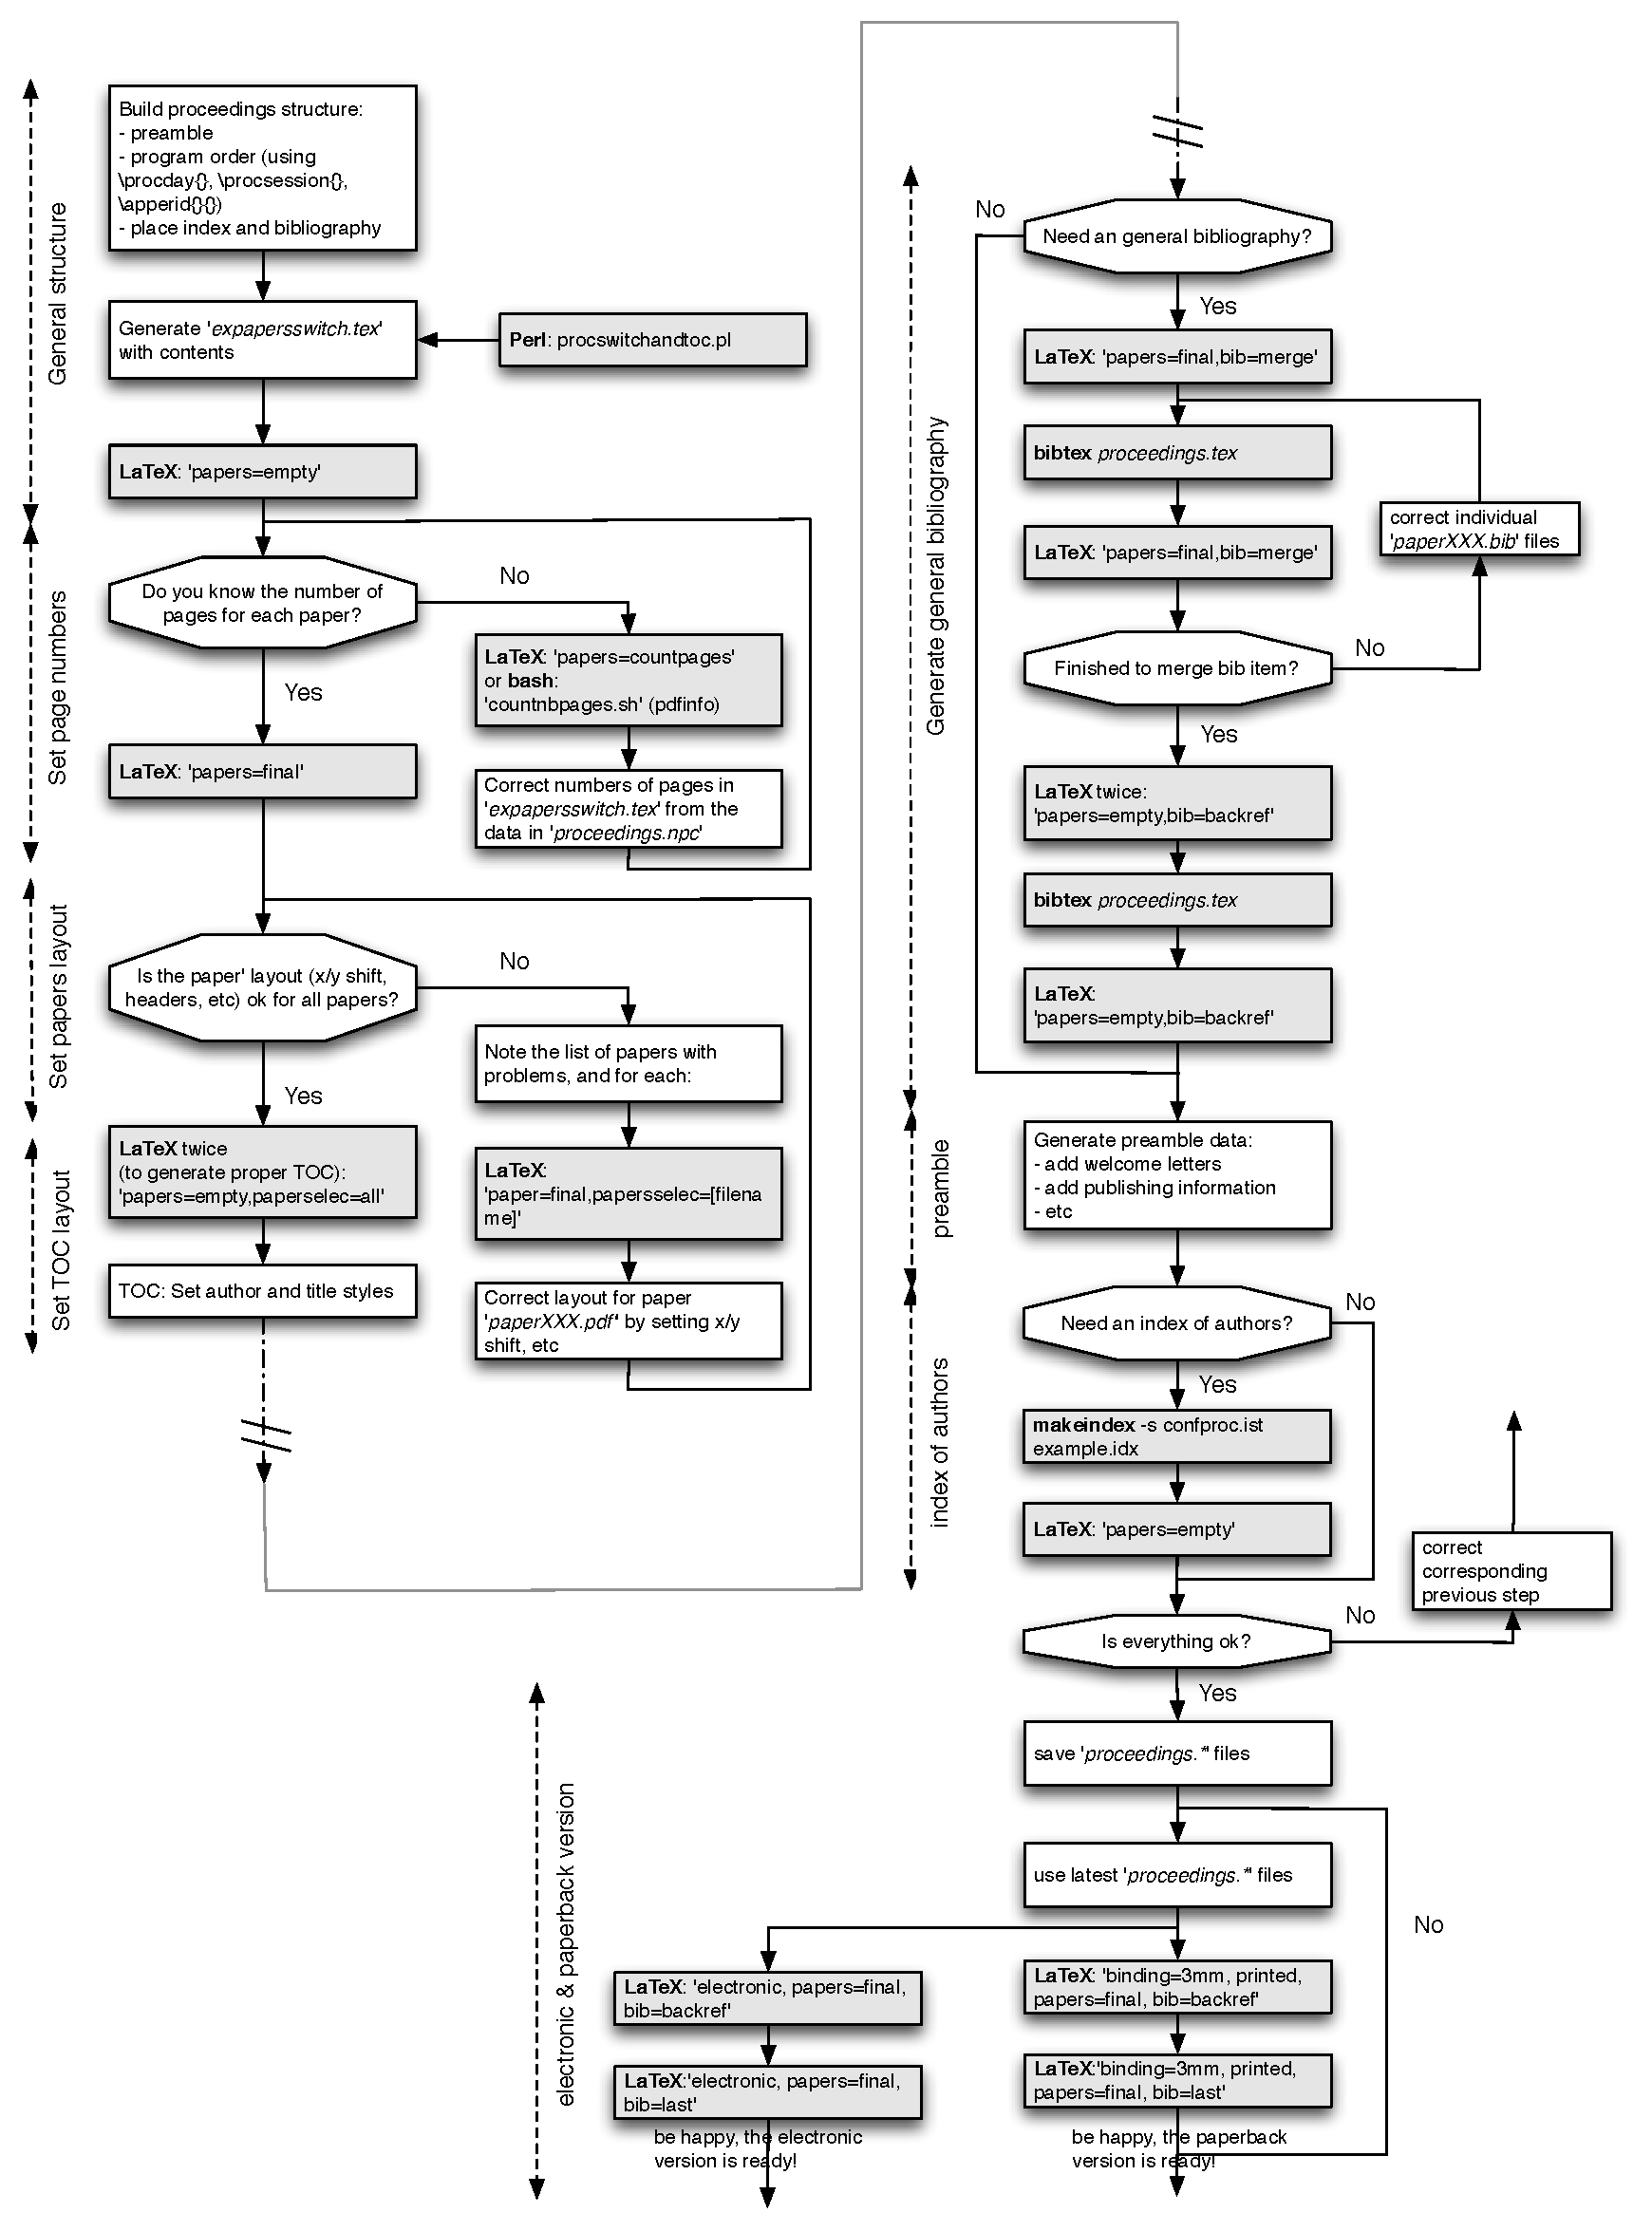
\includegraphics[width=1.1\textwidth]{confproc_diag.pdf} 
%       \caption{Suggested stages to build proceedings}
%       \label{fig:confproc_diag}
%    \end{figure}
%
%    Now that all options and commands to build proceedings are know, we need more insight 
%    about what to do with which option/command and when. This is the purpose of this section, 
%    that proposed some building stages (as depicted in the diagram in Fig.~\ref{fig:confproc_diag}) 
%    to produce both the electronic and paperback final versions of the provided example 
%    proceedings with the following constraints:
%    \begin{itemize}
%      \item the template for papers has a header and footer, so the proceedings must have the same header/footer;
%      \item a general bibliography is used;
%      \item the final PDF papers must be named after their first page number.
%    \end{itemize}
%
%^^A------------------------------------------------------------------------
%    \subsubsection{Generate the program and the paper switch}
%
%    Once the general proceedings structure is there (see the \file{example3optim.tex} file), 
%    the first step is to generate the conference program and its corresponding paper switch:
%        \begin{itemize}
%          \item by hand (read sec.~\ref{sec:ex:paper:switch} for an example);
%          \item using the \file{generateswitch.pl} Perl script described in sec.~\ref{sec:scripts:perl} to generate both the \file{exsessions.tex} and \file{expapersswitch.tex} files from your \file{exprogram.csv} program file.
%        \end{itemize}
%
%
%^^A------------------------------------------------------------------------
%    \subsubsection{Make sure each PDF is fully inserted}\label{sec:compare:page:numbers}
%    At some point, we want to make sure all pages of each paper are inserted. The simplest way
%    is to always use the \Lopt{papers=countpages}, but this is unfortunately very time consuming
%    when working on setting various layout aspects, the program, and also when adding contents
%    to the preamble. Therefore, if using \Lopt{papers=empty} for instance, we want to make sure
%    no paper has been truncated by error. Checking this by hand is a long and fastidious task, so
%    two solutions are offered: the \file{countnbpages.sh} script (see sec.~\ref{sec:scripts:countnbpages}) 
%    and the \file{*.np*} files generated when running \LaTeX\ with either \Lopt{papers=countpages} 
%    or \Lopt{papers=empty}.
%
%    \paragraph{For Unix users:}
%    \begin{enumerate}
%        \item launch once the \file{countnbpages.sh} script (see sec.~\ref{sec:scripts:countnbpages}) to generate \file{example.npc}, which contains each paper's real number of pages;
%        \item run pdflatex onto \file{example.tex} with \LoptDescribe{papers=empty} (faster mode to emulate paper insertion with your settings such as the number of pages); it generates a \file{example.nps} file with the user-defined number of pages;
%        \item compare the content of both files, using
%\begin{verbatim} 
%diff example.nps example.npc
%\end{verbatim} 
%        \item each paper appearing in the \file{diff} command output has a page number discrepancy, that has to be corrected.
%    \end{enumerate}
%    Once all discrepancies have been corrected, re-do this procedure once for a last check,  just in case!  
%    \paragraph{For non-Unix users (sorry, it's much slower!):}
%    \begin{enumerate}
%        \item run pdflatex onto \file{example3optim.tex} with \DescribeMacro{papers=countpages}\Lopt{papers=countpages} (real full paper insertion); it generates \file{example.npc} (real number of pages);
%        \item run pdflatex onto \file{example3optim.tex} with \DescribeMacro{papers=empty}\Lopt{papers=empty} (faster mode to emulate paper insertion with your selected number of pages); it generates \file{example.nps} (supposed number of pages);
%        \item compare both files (with your favorite text editor's `compare file' function).
%    \end{enumerate}
% If some page numbers indicated in \file{expapersswitch.tex} are not identical to the real page number, we just edit the file to correct the error, and can now g on with building the proceedings.
%
%^^A------------------------------------------------------------------------
%    \subsubsection{Changing papers' first page number}
%
%    When the paper template includes the page number in the footer, we need to correct each individual paper's first page number as it appears in the proceedings' table of contents\footnote{When clicking on a paper, the PDF file of this paper will open with the same first page number. Also, if the conference papers are available on the web, knowing the proper page numbers will help readers to properly cite them.}. To do so:
%    \begin{enumerate}
%      \item make at least two runs with the following options:\begin{verbatim}
%\documentclass[a4paper,10pt,twoside,twosidepapers,%
%  compil=last,headers=allpages,movepagenumber,electronic]{confproc}
%\end{verbatim}
%        to include all papers and build a table of contents with proper page numbers.
%      \item prepare each paper for insertion. There are two ways to do this:
%        \begin{enumerate}
%          \item lazy way: use the \verb+\setcounter{page}{XXX}+ command in each paper, with \verb+XXX+ replaced by the real number;
%          \item alternative way (simplifies program changes):  centralize page numbers in the \file{expages.tex} file, organized by the paper ID. Then, the two steps are:
%            \begin{itemize}
%              \item add the following in the preamble of each paper:\begin{verbatim}
%%%
%% This is file `expages.tex',
%% generated with the docstrip utility.
%%
%% The original source files were:
%%
%% confproc.dtx  (with options: `expages')
%% 
%% This is `expages.tex', an example file for the confproc package.
%% Copyright (c) 2011 by Vincent Verfaille <confproc.verfaille@gmail.com>
%% 
%% This file is part of the confproc package.
%% -------------------------------------------
%% 
%% It may be distributed and/or modified under the conditions of the
%% LaTeX Project Public License, either version 1.2 of this license or
%% (at your option) any later version.
%% 
%% The latest version of this license is in
%%   http://www.latex-project.org/lppl.txt
%% and version 1.2 or later is part of all distributions of LaTeX version
%% 1999/12/01 or later.
%% 
%% This file may not be distributed without the original source file
%% `confproc.dtx'.
%% 
%% The list of all files belonging to the confproc package is given in
%% the `readme.txt' file.
%% 
%% For more details, LaTeX the source `confproc.dtx'.
%% 
\newcommand{\setpagenumber}[1]{
  \newcommand{\paperswitch}{#1}
    \ifnum\paperswitch=45 {\setcounter{page}{1}}\fi
    \ifnum\paperswitch=21 {\setcounter{page}{7}}\fi
    \ifnum\paperswitch=27 {\setcounter{page}{13}}\fi
    \ifnum\paperswitch=33 {\setcounter{page}{17}}\fi
    \ifnum\paperswitch=75 {\setcounter{page}{23}}\fi
}
\setpagenumber{04}
%\end{verbatim}
%               Here, the ID paper is \verb+04+, and has to be updated for each paper.
%              \item update the \file{expages.tex} file for each paper: set its first page number as it appears in the table of contents.
%            \end{itemize}
%            By doing so, we can update the program to re-build the table of contents as many times as wanted, without having to re-edit each paper. 
%        \end{enumerate}
%      \item once the program and the corresponding paper order are ok, (re)generate each paper independently with proper first page number (using the \file{buildpapers.sh} script in sec.~\ref{sec:scripts:buildpapers}); 
%      \item check that no error was made when numbering the first page. Run \LaTeX\ with at least the \Lopt{headers=allpages,movepagenumber} options. In case of error, re-do step 2--3 till the page numbers are ok.
%    \end{enumerate}
%
%^^A------------------------------------------------------------------------
%    \subsubsection{Renaming papers}
%
%    Renaming all papers according to their first page number (\eg{} \file{p\_NNN.pdf} if only PDF files are renamed) is very helpful to ensure the proceedings' CD version is ISO compliant, and has file names with less than 8 characters (+ extensions). This can only be done once the program is definitive. Then file names can be changed accordingly in the \file{.csv} file; the \file{expapersswitch.tex} file has to be re-generated, and the proceedings  rebuilt. It is easily done using the Unix scripts.
%
%
%
%^^A =================================================================
%    \subsection{Quality and production}
%
%    We present here some other ideas dealing with the production and the quality of the proceedings. Indeed, to provide the best possible quality proceedings, individual papers may be edited (see sec.~\ref{sec:misc:editing}), which can be simplified by sending notes to authors before they submit the final version (see sec.~\ref{sec:misc:notes}). Using only \LaTeX{} to typeset may require to convert some Word files to \LaTeX, in the case where the proceedings templates are provided in the 2 formats to authors (see sec.~\ref{sec:misc:word2latex}). The last comments are about the graphical quality (sec.~\ref{sec:misc:graph:quality}) and the necessary font embedding in the PDF images (see sec.~\ref{sec:misc:images:fonts}).
%
%^^A------------------------------------------------------------------------
%    \subsubsection{Editing the papers}\label{sec:misc:editing}
%
%    To provide the best possible quality proceedings for DAFx-06, each individual paper was edited by checking the following items (non-exhaustive list):
%    \begin{itemize}
%        \item proper page format used (US letter instead of A4 format), as the authors were from various continents around the worlds;
%        \item break the title line at the right place using  \verb+\break+;
%        \item affiliation type is properly indicated;
%        \item affiliation is properly layed out;
%        \item author's email exists and works;
%        \item captions are italic, with a ``.'' at the end;
%        \item all figures are referenced in the text;
%        \item bibliographic items have a volume and number, as well as page number or preprint number (AES convention);
%        \item bibliographic items use generally defined strings, and are identical each time they are cited;
%        \item math units: Physics convention is roman, not italic (\ie{} not LaTeX's math style). Ex: $5$ Hz, and not $5Hz$.
%    \end{itemize}
%
%    \noindent So as to ensure papers look uniform as possible, we changed for each:
%    \begin{itemize}
%        \item the URL font to sans-serif, as its default font is too wide. We added the following command in the preamble of each paper:\\
%            \verb+\usepackage{url}\urlstyle{sf}+
%        \item all \verb+\href{}{}+ commands related to URL (\ie{} all except emails) where converted to URL, as it is more apropriated (it does the hyphenations for you and most of the time it does it better).
%    \end{itemize}
%
%    \noindent Some not-so-minor comments:
%    \begin{itemize}
%        \item to do a valid line break in the paper title (at least with the \file{dafx06.sty} style, but not only) use  \verb+\break+, instead of \verb+\newline+, \verb+\\+, or \verb+\linebreak+ (that creates unbalanced titles). That way, it works similarly for both the title and the pdftitle in the metadata. 
%        \item using the \package{balance.sty} package allows to well balance the last page, which is especially useful for the bibliography.
%    \end{itemize}
%
%^^A------------------------------------------------------------------------
%    \subsubsection{Sending editing notes to authors to improve the layout quality}\label{sec:misc:notes}
%
%    In order to improve aspects of the quality of the proceedings, we listed many common errors and gave a feedback to authors of all accepted papers, that they were kindly asked to take care of. This is how we proceeded:
%    \begin{enumerate}
%        \item examine all papers and list the common errors and electronic paper info (PDF version, PDF generator, valid hyperref, etc.) (10h);
%        \item in an \file{.csv} file, indicate all problems, paper's title, index and author's email (0.5h);
%        \item column by column, fill in the data (30h) with errors detected in each paper;
%        \item use a combination of Perl script and an AppleScript to convert info in this file into usual sentences and indications of what to do in order to improve the paper quality (4h), and then into a series of emails, ready to be sent to authors (4h). 
%    \end{enumerate}
%    N.B.: Those scripts are not provided in the package, but can be obtained on demand.
%
%
%^^A------------------------------------------------------------------------
%    \subsubsection{Manual Word to \LaTeX\ conversion}\label{sec:misc:word2latex}
%
%    To automatize all the processes in proceedings making, we may want to convert  all non-\LaTeX\ generated documents into \LaTeX{} documents. If that cannot be asked to the conference authors, we need to do it ourselves. Here is an example of the steps to follow:
%    \begin{enumerate}
%        \item copy and paste the whole text;
%        \item update the header (author, title, affiliation);
%        \item add sections, subsections, etc. according to the original text;\\
%                 update labels and references for sections, subsections, etc.;
%        \item insert figures and tables with the proceedings template style;\\
%                 update labels and references for figures and tables;
%        \item update captions with the proceedings template style;
%        \item edit equations (inside the text and as separated formulae);\\
%                update labels and references for equations ;
%        \item replace all Word quotes  ^^A(double “”‟ and single ‛' quotes) 
%           by \LaTeX\ quotes (double ``'', and single `' quotes) to avoid they disappear (Unicode-related issue);
%        \item correct any specific formatting such as italic, capitals, bold, etc;
%        \item remove useless hyphenations ``-'' produced as line breaks by Word;
%        \item replace remaining hyphens by the proper corresponding one: dash `-' (hyphen), semi-quadratin `--' (ex: number range) and quadratin `---'.
%    \end{enumerate}
%
%^^A------------------------------------------------------------------------
%    \subsubsection{How to ensure the graphical quality?}\label{sec:misc:graph:quality}
%
%    The best way to ensure excellent quality for you graphics in the electronic version of you proceedings consists in using vectorial images, \ie{} postscript (\file{.ps} or \file{.eps}) or \file{.pdf} files. It should be the same for the printed version, except that the font problem with Matlab described in sec.~\ref{sec:misc:images:fonts} may imply to convert vectorial images to bitmap images (such as \file{.png} or \file{.gif}).
%
%
%
%^^A------------------------------------------------------------------------
%    \subsubsection{How to ensure your fonts are embedded in the PDF?}\label{sec:misc:images:fonts}
%
%   Various important things have to be checked to ensure a great PDF file quality. (Please read  \href{http://www.prepressure.com/pdf/basics/preflight}{www.prepressure.com/pdf/basics/preflight} for more information). 
%     One of these important things is the font embedding. 
%    If not checked, you may end up with a document where fonts will disappear and be replaced by random characters (which are not random in fact)\footnote{Indeed, when printing on a system that is not yours (\eg{} in a professional print center), the printer may be set such as not to replace a missing font by a similar one. This is why, Matlab text can be totally scrapped, replaced by other numbers, letters, and so on!}.
%    Unfortunately for non-experts user of Matlab, the system fonts such as Arial or Helvetica are not embedded by default in the \file{.pdf} nor in the \file{.eps} file. This can be checked by converting any of the two into another format using Ghostscript. For instance, converting a \file{.pdf} to \file{.ps} using \file{pdf2ps} will show the following log info:\begin{verbatim}
%   **** Warning: Fonts with Subtype = /TrueType should be embedded.
%                 The following fonts were not embedded:
%                        Arial-ItalicMT
%                        ArialMT
%
%   **** This file had errors that were repaired or ignored.
%   **** The file was produced by:
%   **** >>>> pdfTeX-0.14h <<<<
%   **** Please notify the author of the software that produced this
%   **** file that it does not conform to Adobe's published PDF
%   **** specification.
%\end{verbatim}
%    This can also be checked by processing a PDF files produced by Matlab using Acrobat Distiller (\$), and you will get the same errors...
%
%    A way to correct this in Matlab is use the \file{print\_pdf.m}\footnote{get it at: \href{http://www.mathworks.com/matlabcentral/fileexchange/22018-printpdf}{\sf www.mathworks.com/matlabcentral/fileexchange/22018-printpdf})} file by \person{Oliver Woodford}  to save the figure as PDF with embedded fonts.
%
%    If you cannot have it fixed by the author, then you need to use Acrobat Professional to do the job for you. 
%    Utilities like \file{pdfinfo} and \file{pdffonts} are helpful to detect such problems as well as missing bounding boxes, with commands like:\\
%    \texttt{pdffonts [filename.pdf]}\\
%    \texttt{pdfinfo -box [filename.pdf]}
%
%
%
%^^A\changes{0.1c}{2007/07/30}{Customization: \file{confproc.cfg}}
%
%    \color{black}
%
%
%\changes{0.6}{\datevzdsix}{Doc: moved scripts after the full example and before implementation}
%^^A\changes{0.2f}{2007/09/05}{Scripts: Unix `buildcls' script added}
%^^A\changes{0.2g}{2007/09/07}{Scripts: Unix `buildcls' script shorten}
%^^A\changes{0.2g}{2007/09/07}{Scripts: Unix `buildcls' script with chmod on the Perl script, + example of use of the script}
%^^A\changes{0.2h}{2007/09/12}{Scripts: Unix `buildcls' script moves example files in `example/'}
%^^A\changes{0.2i}{2007/09/24}{Scripts: Unix `buildcls' script moves the index style `confproc.ist' in `example/'}
%
%
%^^A =================================================================
%    \section{Various scripts and utilities to save time} \label{sec:scripts}
%
%^^A =================================================================
%    \subsection{\file{buildcls.sh}: Build the class documentation and files}
%
%    \begin{description}
%      \item[Name] \file{buildcls.sh}
%      \item[Type] Unix/bash script
%      \item [Purpose] generates the class files and documentation, and prepares the example-related files.  
%      \item [Note] first set the path to \LaTeXe\ binaries before using it!
%    \end{description}
%    \begin{macrocode}
%<*buildcls>
#!/bin/sh

wd=`pwd`

%    \end{macrocode}
%    First, you may set the path to \LaTeXe\ binaries:
%    \begin{macrocode}
#-- set path to LaTeX binaries
LaPath="/usr/texbin/" # TeXLive

%    \end{macrocode}
%    and then, only if necessary, change the names to the \LaTeX{} compilers:
%    \begin{macrocode}
#-- set names of LaTeX and related compilers
Latex=$LaPath"pdflatex"
Index=$LaPath"makeindex"
%    \end{macrocode}
%    as well as the document and example target names:
%    \begin{macrocode}
Target="confproc"  #- set document's name
extarget="example/" #- set the example folder name

%    \end{macrocode}
%    We can start building the documentation and the \file{.ins} file:
%    \begin{macrocode}
#-- build doc, class and example files
$Latex $Target.dtx #- build doc. and .ins file
$Latex $Target.ins #- build class and example files

%    \end{macrocode}
%    We then rename the bibliography style (HACK: the file is generated under the \file{newapave2.sty}, because  if there already exist a \file{newapave.sty} on your system, it will not be generated again under that name; we now have to properly rename it):
%    \begin{macrocode}
#-- HACK: rename newapave2.sty
mv newapave2.sty newapave.sty

%    \end{macrocode}
%    Once it is done, we can finish the documentation. this full sequence is only necessary if you generate the implementation, index and changes history:
%    \begin{macrocode}
cd $wd/
#-- finish to build the documentation
$Latex $Target.dtx #- re-run doc for toc update
$Latex $Target.dtx #- re-run doc for proper back-references
$Index -s gind.ist $Target  #- with \CodelineIndex of \PageIndex
$Index -s gglo.ist -o $Target.gls $Target.glo  #- with \RecordChanges
$Latex $Target.dtx #- insert index & list of changes, re-number
$Latex $Target.dtx #- last run with proper page numbers

%    \end{macrocode}
%    Since there are 2 scripts, one to install (this one) and one to clean up all the mess (mainly used by me during building tests), we also prepare the latter:
%    \begin{macrocode}
#-- prepare scripts for cleaning package
cd $wd
chmod +x cleancls.sh

%    \end{macrocode}
%    We then create the example folder and move all related files thanks to the \file{prepareexample.sh} script (sec. \ref{sec:script:prepareexample}): 
%    \begin{macrocode}
#-- prepare scripts for building example
chmod +x prepareexample.sh
./prepareexample.sh

%    \end{macrocode}
%    By uncommenting the last line, you will also build the example!
%    \begin{macrocode}
#-- build example
cd $extarget
#./buildproc.sh
%</buildcls>
%    \end{macrocode}
%    This script is generated by the first \LaTeX\ run on \package{confproc.dtx}. You then have to change its permission in the \verb+bash+ shell to make it executable:\begin{verbatim}
%chmod +x buildcls
%\end{verbatim}
%    Then, you can run it from the \verb+bash+ shell:\begin{verbatim}
%./buildcls
%\end{verbatim}
%
%
%
%
%^^A\changes{0.2f}{2007/09/05}{Scripts: Unix `cleancls' script added}
%^^A\changes{0.2g}{2007/09/07}{Scripts: Unix `cleancls' script shorten}
%^^A =================================================================
%    \subsection{\file{cleancls.sh}: Clean up the class folder}
%
%    \begin{description}
%      \item[Name] \file{cleancls.sh}
%      \item[Type] Unix/bash script
%      \item [Purpose] cleans up the folder where the class was generated.
%    \end{description}
%    \begin{macrocode}
%<*cleancls>
#!/bin/sh

%    \end{macrocode}
%    Create a back up folder:
%    \begin{macrocode}
mkdir backup #--- move the files to be kept
%    \end{macrocode}
%    Move original class documentation materials:
%    \begin{macrocode}
mv confproc.dtx backup/
mv confproc_diag.pdf backup/
mv confproc-short.tex backup/
mv confproc-short.pdf backup/
%    \end{macrocode}
%    Move building and cleaning scripts:
%    \begin{macrocode}
mv buildcls.sh backup/
cp cleancls.sh backup/
%    \end{macrocode}
%    Cleanup and place back the original minimal file set:
%    \begin{macrocode}
rm *.* #--- clean up!
mv backup/* . #--- move the backed up files
rm -r backup #--- remove the temporary backup folder
%</cleancls>
%    \end{macrocode}
%    You may want to use it to re-generate the whole package from the \file{.dtx} file.
%    Note that this script too is generated by the first \LaTeX\ run on the \package{confproc.dtx} file.
%
%
%
%^^A =================================================================
%    \subsection{\file{prepareexample.sh}: Prepare the example files, scripts and folders}\label{sec:script:prepareexample}
%
%    \begin{description}
%      \item[Name] \file{prepareexample.sh}
%      \item[Type] Unix/bash script
%      \item [Purpose] prepares the example-related files, scripts and folders
%      \item [Note] first set the path to \LaTeXe\ binaries before using it!
%    \end{description}
%    \begin{macrocode}
%    \changes{0.7}{2010/08/05}{added \file{prepareexample.sh}}
%<*prepareexample>
#!/bin/sh

wd=`pwd`

%    \end{macrocode}
%    Set the example folder name:
%    \begin{macrocode}
extarget="example" #- set the example folder name

%    \end{macrocode}
%    Then create the example folder: 
%    \begin{macrocode}
#-- prepare scripts for building example
mkdir $extarget #- create the folder

#-- generate the program session files
perl generateswitch.pl<exprogram.csv

%    \end{macrocode}
%    and move the example-related files and scripts:
%    \begin{macrocode}
mv ex*.* $extarget/ #- move all other example files into proper folder
mv buildproc* $extarget/ #- move scripts into it
mv buildcppdfpapers* $extarget/
mv buildpapers* $extarget/
mv countnbpages.sh $extarget/
mv generateswitch.pl $extarget/
mv papersinfo.sh $extarget/
mv paperssplitpreamble.sh $extarget/
mv removeLaTeXcmds.sh $extarget/

%    \end{macrocode}
%    Also, copy folder and files that are common to the class documentation and the example:
%    \begin{macrocode}
cp -r pictures $extarget/ #- copy pictures into it
cp -r papers $extarget/ #- copy papers into it
cp confproc.cls $extarget/ #- copy the class into it
cp confproc*.ist $extarget/ #- copy the index style into it
cp newapave* $extarget/ #- copy the newapave bib style files

%    \end{macrocode}
%    Move the \file{expages.tex} generated file to the right place, and prepare the \package{pdftk} information folder:
%    \begin{macrocode}
#-- prepare building scripts and generate needed directories
cd $wd/$extarget
mkdir pdftk_info/
mv expages.tex papers/

%    \end{macrocode}
%    Change the permission of the example-related scripts:
%    \begin{macrocode}
cd $wd/$extarget
chmod +x buildproc*
chmod +x generateswitch.pl
chmod +x exportIndividualPDFs.sh
chmod +x papersinfo.sh 
chmod +x paperssplitpreamble.sh 
cd ..

%    \end{macrocode}
%    By uncommenting the last line, we also build the example!
%    \begin{macrocode}
#-- build example
cd $wd/$extarget
#./buildproc.sh
%</prepareexample>
%    \end{macrocode}
%    \noindent N.B.: This script is generated by the first \LaTeX\ run on \package{confproc.dtx}. You then have to change its permission in the \verb+bash+ shell to make it executable:\begin{verbatim}
% chmod +x prepareexample.sh # change its permissions
%\end{verbatim}
%    Then, you can run it from the \verb+bash+ shell:\begin{verbatim}
%./prepareexample.sh
%\end{verbatim}
%
%
%
%^^A =================================================================
%    \subsection{\file{generateswitch.pl}: Generate the paper switch and program [Perl]}
%    \label{sec:scripts:perl}
%
%^^A\changes{0.2c}{2007/08/17}{Scripts: Perl script 'generateswitch.pl' to generate 'paperswitch.tex' and 'sessions.tex' added}
%^^A\changes{0.2d}{2007/08/18}{Scripts: Perl script to generate 'generateswitch.pl' added}
%^^A\changes{0.2d}{2007/08/18}{Scripts: Perl script 'generateswitch.pl' modified to insert bookmarks, and text shorten}
%^^A\changes{0.2d}{2007/08/20}{Scripts: Perl script modified and authors pdfboomarks added}
%^^A\changes{0.2g}{2007/09/07}{Scripts: changing input file line break style (Unix instead of Max)}
%^^A\changes{0.2h}{2007/09/12}{Scripts: Perl script is case insensitive for session names 9and has more options)}
%^^A =================================================================
%^^A   Here is the creation of the procwitchandtoc.pl file, part of the example.
%^^A   It is written on first LaTeX run if it does not already exist
%^^A =================================================================
%
%    \begin{description}
%      \item[Name] \file{generateswitch.pl}
%      \item[Type] Perl script
%      \item [Purpose] generates TOC-related example files: paper switch in \file{expapersswitch.tex} and papers order by sessions and days in \file{exsessions.tex}.
%      \item to use it, type in a bash terminal: \verb+perl generateswitch.pl<exprogram.csv+ (or any other program file).
%    \end{description}
%
%    \begin{macrocode}
%<*generateswitch>
#!/usr/bin/perl -w

# generateswitch.pl
#    created as dafxproctoc.pl by Marc Zadel, 2006-04-28
#    modified for confproc.cls by Vincent Verfaille, 2007-08-08 (v0.4) & 2009-10-30 (v0.7)
# Execute as
# ./generateswitch.pl < intputfile.txt >

use strict;
use Text::ParseWords;
open(SWI, ">expapersswitch.tex"); #open for write, overwrite
open(SESSIONS, ">exsessions.tex"); #open for write, overwrite

# ----- Configuration
# field separator for the input file
my $fieldseparator=',';

# mac line endings: "\r"  / Unix line endings: :\n"
$/ = "\n";  # line endings for the input file
$\ = "\n";  # line endings for the output file

# ----- Subroutines
# -- split one line of input into a hash with named fields
sub parseinputline {
  my ($inputline) = @_;

  # escape single quotes on the input line: they interfere with quotewords()'s
  # quote handling (ie, they start to quote stuff)
  $inputline =~ s/'/\\'/g;

  # parse the input line
  my @wordlist = &quotewords($fieldseparator, 0, $inputline);

  # replace accented characters with latex escaped equivalents. Use it after
  # quotewords() so the '\' don't get interpreted by quotewords() as escapes
  foreach my $word ( @wordlist ) {
    if ( $word ) { $word = &latexifyaccentedcharacters($word); }
  }

  # extract the fields into local variables. Author names stored as a list
  my ($type, $number, $pcdecision, $nbpages, $title, $filename,
      $generatedfrom, $cite) = @wordlist;

  # remove the first 8 elements (just parsed out), leaving only author names.
  # reminder: list of 8 scalars, though some may be "" if less than 4 authors
  splice( @wordlist, 0, 8 );

  # store the author names as a list of lists. We end up with a list that looks
  #  like ((Udo,Zoelzer),(Daniel,Arfib))
  my @authors = ();
  while ( $wordlist[0] ) {
    push( @authors, [splice( @wordlist, 0, 2 )] );
    # "splice( @wordlist, 0, 2 )": cuts the first 2 scalars off of @wordlist
    # and returns them; calling [splice(@wordlist,0,2)] returns a *reference*
    # to a list containing the first two scalars. (see perldoc perldsc.)
  }

  # create a hash reference containing the named fields and return it
  my $fields = {
    type    => $type,
    number    => $number,
    pcdecision  => $pcdecision,
    nbpages     => $nbpages,
    title     => $title,
    generatedfrom => $generatedfrom,
    filename  => $filename,
    cite    => $cite,
    authors   => \@authors,
  };
  return $fields;
}

# -- takes a string in Mac OS Roman encoding and encode the accented
#  characters with latex escapes (only for a subset of available characters).
sub latexifyaccentedcharacters {
  # for mapping between unicode and mac os western encoding, see:
  # http://www.unicode.org/Public/MAPPINGS/VENDORS/APPLE/ROMAN.TXT
  my ($inputstring) = @_;
  $inputstring =~ s/\x8a/\\"a/g;  # \"a: unicode 0xe4, mac os western 0x8a
  $inputstring =~ s/\x87/\\'a/g;  # \'a: unicode 0xe9, mac os western 0x87
  $inputstring =~ s/\x88/\\`a/g;  # \`a: unicode 0xe8, mac os western 0x88
  $inputstring =~ s/\x8e/\\'e/g;  # \'e: unicode 0xe9, mac os western 0x8e
  $inputstring =~ s/\x8f/\\`e/g;  # \`e: unicode 0xe8, mac os western 0x8f
  $inputstring =~ s/\x91/\\"e/g;  # \"e: unicode 0xeb, mac os western 0x91
  $inputstring =~ s/\x97/\\'o/g;  # \'o: unicode 0xf3, mac os western 0x97
  $inputstring =~ s/\x98/\\`o/g;  # \`o: unicode 0xf2, mac os western 0x98
  $inputstring =~ s/\x9a/\\"o/g;  # \"o: unicode 0xf6, mac os western 0x9a
  $inputstring =~ s/\x99/\\^o/g;  # \^o: unicode 0xf4, mac os western 0x99
  $inputstring =~ s/\xbf/\\o /g;  # \o:  unicode 0xf8, mac os western 0xbf
  $inputstring =~ s/\x96/\\~n /g;  # \~n:  unicode 0xF1, mac os western 0x96
  $inputstring =~ s/\x94/\\^{\\i}/g;  # \^{\i}: unicode 0xee, mac os western 0x94
  $inputstring =~ s/\x/\\i/g;  # \i: unicode , mac os western
  $inputstring =~ s/\x9f/\\"u/g;  # \"u: unicode 0xfc, mac os western 0x9f
  $inputstring =~ s/\x5c/\\/g;  # \: unicode 0x5C, mac os western 0x5C

  return $inputstring;
}

# -- output the information for a day
sub outputdaylatex {
  my ($fields) = @_;
  my $sessiontitle = $fields->{'title'};
  open(SESSIONS, ">>exsessions.tex"); #open for append
  print SESSIONS ' ';
  print SESSIONS '%%%== Day';
  print SESSIONS '\procday{', $sessiontitle, '}'
}

# -- output the information for a session line
sub outputsessionlatex {
  my ($fields) = @_;
  my $sessiontitle = $fields->{'title'};
  open(SESSIONS, ">>exsessions.tex"); #open for append
  print SESSIONS ' ';
  print SESSIONS '%%%-- session';
  print SESSIONS '\session{', $sessiontitle, '}'
}

# -- in: ref. to a list of lists of author names ((Udo,Zoelzer),(Daniel,Arfib))
# out: ref. to a Perl list w/ entries "Udo Zoelzer" and "Daniel Arfib" (no quotes)
sub authorsbyfirstname {
  my ($authors) = @_;
  # generate a list of full "first last" author names
  my @authorlistbyfirstname = map { "$_->[0] $_->[1]" } @$authors;
  return \@authorlistbyfirstname; # return a ref. to the new list of authors
}

# -- in: ref. to a list of lists of author names ((Udo,Zoelzer),(Daniel,Arfib))
# out: ref. to a Perl list w/ entries "Zoelzer, Udo" and "Arfib, Daniel"
sub authorsbysurname {
  my ($authors) = @_;
  # generate a list of authors with surnames written first
  my @authorlistbysurname = map { "$_->[1], $_->[0]" } @$authors;
  return \@authorlistbysurname; # return a ref. to the new list of authors
}

# -- in: ref. to a list of author names: "Zoelzer, Udo" and "Arfib, Daniel"
# out: LaTeX index entries: "\index{Zoelzer, Udo}\index{Arfib, Daniel}"
sub genindex {
  my ($authorsbysurname) = @_;
  my @indexentries = map { "\\index{$_}" } @$authorsbysurname;
  return join('', @indexentries);
}

# -- in: ref. to a list of author names: "Zoelzer, Udo" and "Arfib, Daniel"
# out: bookmarks cmds: "\pdfbookmark[2]{Udo Zoelzer}{#2.Udo Zoelzer}
# \pdfbookmark[2]{Daniel Arfib}{#2.Daniel Arfib}"
sub genbookmark {
  my ($authorsbyfirstname) = @_;
  my @indexentries = map { "\\pdfbookmark[2]{$_}{#2.$_}" }
      @$authorsbyfirstname;
  return join('', @indexentries);
}

# -- output the information for a paper line
sub outputpaperlatex {
  my ($fields) = @_;
  open(SWI, ">>expapersswitch.tex"); #open for append
  print SWI '%======= PAPER ID = ', $fields->{'number'}, ' =======';
  print SWI '\ifnum\paperswitch=', $fields->{'number'};
  print SWI '  \procpaper[xshift=\LaTeXxShift{}, yshift=\LaTeXyShift{}, npages=',
    $fields->{'nbpages'}, ', switch=\paperswitch,%';
  print SWI '    title={', $fields->{'title'}, '},% paper title';
  print SWI '    author={', join( ', ', @{&authorsbyfirstname($fields->{'authors'})}),
  '},% list of authors';
  print SWI '    index={', &genindex(&authorsbysurname($fields->{'authors'})),
  '},% authors index entries';
  print SWI '    cite={', $fields->{'cite'}, '},% cited bib items';
#  print SWI '  {#2}{\paperbookmark}';
  print SWI '    bookmark={', &genbookmark(&authorsbyfirstname($fields->{'authors'})),'}% for PDF bookmark structure';
  print SWI '  ]{#2}';
  print SWI '\fi';
  print SWI ' ';
  open(SESSIONS, ">>exsessions.tex"); #open for write, overwrite
  print SESSIONS '\paperid{', $fields->{'number'}, '}{', $fields->{'filename'}, '}';
}

# ----- Main
# FIXME: parse a line, and confirm that all of the fields are set up properly
# --> correct number of fields, and the fields have the correct values
open(SWI, ">>expapersswitch.tex"); #open for write, overwrite
print SWI '\newcommand{\paperid}[2]{';
print SWI ' ';
print SWI '\renewcommand{\paperswitch}{#1}';
print SWI ' ';

while ( <> ) {
  chomp; # clear the newline character from the end of the line
  my $fields = &parseinputline($_);   # parse the line into fields
  # take some action depending on what type of line it is; case insensitive
  if ( lc($fields->{'type'}) eq lc('day') ) {
  &outputdaylatex($fields);
  } elsif ( lc($fields->{'type'}) eq lc('session')
      || lc($fields->{'type'}) eq lc('paper session')
      || lc($fields->{'type'}) eq lc('demo session')
      || lc($fields->{'type'}) eq lc('poster session') ) {
  &outputsessionlatex($fields);
  } elsif ( lc($fields->{'type'}) eq lc('oral')
      || lc($fields->{'type'}) eq lc('paper')
      || lc($fields->{'type'}) eq lc('demo')
      || lc($fields->{'type'}) eq lc('poster') ) {
  &outputpaperlatex($fields);
  } elsif ( lc($fields->{'type'}) eq lc('Type')) {
  } else { print '!!! a day, session or paper (',
      $fields->{'type'},') is lost by the script...';
  }
open(SWI, ">>expapersswitch.tex"); #open for append
}
print SWI '}';
close(SWI);
close(SESSIONS);
%</generateswitch>
%    \end{macrocode}
%
%
%
%^^A =================================================================
%    \subsection{\file{buildproc.sh}: Build the proceedings}\label{sec:confproc:compil:script}\label{sec:scripts:buildproc}
%
%    \begin{description}
%      \item[Name] \file{buildproc.sh}
%      \item[Type] Unix/bash script
%      \item[Purpose] describes all compilation steps to produce the final version of the proceedings
%      \item[Note] This script is the most important!
%    \end{description}
%    This script applies several \LaTeX{} runs to create valid table of content, index, bibliography, index of authors, and proper back references from the bibliography. It also manages the renaming of the class insertion file, so we do not need anymore to run a last time by hand after changing the \Lopt{compil=backref} option to \Lopt{compil=last} (as this option change, and others, are in the \file{exclasspre.tex} and \file{exclasslast.tex} files).
%
%
%^^A\changes{0.1d}{2007/08/01}{Adding the buildproc script creation.}
%^^A =================================================================
%^^A   Here is the creation of the buildproc script file, part of the example.
%^^A   It is written on first LaTeX run if it does not already exist
%^^A =================================================================
%
%    \begin{macrocode}
%<*buildproc>
#!/bin/sh

%    \end{macrocode}
%    We set the user-dependent  the original file name (no extension):
%    \begin{macrocode}
#--- set user dependent file name
TEXFILE="example3optim"
%    \end{macrocode}
%    Let us now set system-dependent variables: the path the the \LaTeX{} distribution as well as the binaries:
%    \begin{macrocode}
#--- set system-dependent variables
LATEXPATH="/usr/texbin/" # for TexLive
#--- set compilers' paths
PDFLATEX=$LATEXPATH"pdflatex"
BIBTEX=$LATEXPATH"bibtex"
MAKEINDEX=$LATEXPATH"makeindex"
mkdir pdftk_info/

%    \end{macrocode}
%    \begin{itemize}
%      \item we copy the class options (including \Lopt{bib=backref}) to the file called by the core file:
%    \end{itemize}
%    \begin{macrocode}
#--- class settings: "empty" option and binding
cp exclasspre.tex exclass.tex
%    \end{macrocode}

%    \begin{itemize}
%      \item we run \LaTeX{} once to generate the table of contents:
%    \end{itemize}
%    \begin{macrocode}
#--- Compile
separator='___________________________________________________'
echo; echo; echo; echo; echo; echo; echo $separator; echo $separator;
echo '*** PdfLaTeX: create toc (1/6) ***'
$PDFLATEX  $TEXFILE.tex

%    \end{macrocode}
%    \begin{itemize}
%      \item we run bib\TeX{} once to generate the bibliography:
%    \end{itemize}
%    \begin{macrocode}
echo; echo; echo; echo; echo; echo; echo $separator; echo $separator;
echo '*** Bibtex: generate the general biblio. (2/6) ***'
$BIBTEX $TEXFILE

%    \end{macrocode}
%    \begin{itemize}
%      \item we run \package{makeindex} once to generate the author index:
%    \end{itemize}
%    \begin{macrocode}
echo; echo; echo; echo; echo; echo; echo $separator; echo $separator;
echo '*** Makeindex: create index of authors (3/6) ***'
$MAKEINDEX -s confproc2.ist $TEXFILE.idx

%    \end{macrocode}
%    \begin{itemize}
%      \item we run \LaTeX{} once to insert the table of contents, index and bibliography, and update their page numbers for next run:
%    \end{itemize}
%    \begin{macrocode}
echo; echo; echo; echo; echo; echo; echo $separator; echo $separator;
echo '*** PdfLaTeX: add toc + insert index and bibliography (4/6) ***'
$PDFLATEX  $TEXFILE.tex

%    \end{macrocode}
%    \begin{itemize}
%      \item we run \LaTeX{} once again to insert update page numbers in the table of contents, index and bibliography:
%    \end{itemize}
%    \begin{macrocode}
echo; echo; echo; echo; echo; echo; echo $separator; echo $separator;
echo '*** PdfLaTeX: createupdate toc, index and bib page numbers (5/6) ***'
$PDFLATEX $TEXFILE.tex

%    \end{macrocode}
%    \begin{itemize}
%      \item we do the final  \LaTeX{} run:
%    \end{itemize}
%    \begin{macrocode}
echo; echo; echo; echo; echo; echo; echo $separator; echo $separator;
echo '*** PdfLaTeX: mod. class insertion, for proper PDF links for full papers (6/6) ***'
$PDFLATEX $TEXFILE.tex
%</buildproc>
%    \end{macrocode}
%
%
%
%^^A =================================================================
%    \subsection{\file{buildprocelpb.sh}: Generate both paperback and electronic final versions}\label{sec:scripts:buildprocelpb}
%
%    \begin{description}
%      \item[Name] \file{buildprocelpb.sh}
%      \item[Type] Unix/bash script
%      \item[Purpose] describes all compilation steps to produce the final version of both paperback and electronic proceedings
%      \item[Note] This script helps to automatize the whole production process; its is described/commented as an incrementation from \file{buildproc.sh}.
%    \end{description}
%
%
%^^A =================================================================
%^^A   Here is the creation of the buildprocelpb.sh script file, part of the example.
%^^A   It is written on first LaTeX run if it does not already exist
%^^A =================================================================
%\changes{0.6}{\datevzdsix}{added \file{buildproc2.sh}}
%\changes{0.7}{2010/08/05}{renamed \file{buildproc2.sh} into \file{buildprocelpb.sh}}
%
%  We first set the user-dependent file names and folders, namely: 
%    \begin{macrocode}
%    \changes{0.7}{2010/08/05}{added \file{buildprocelpb.sh}}
%    \color{black!50}
%<*buildprocelpb>
#!/bin/bash

#--- set user dependent file name
%    \end{macrocode}
%    \color{black}
%    \begin{itemize}
%      \item the original file name (no extension):
%    \end{itemize}
%    \begin{macrocode}
INTEXFILE="example4optim"
%    \end{macrocode}
%    \begin{itemize}
%      \item the target file name (no extension):
%    \end{itemize}
%    \begin{macrocode}
TEXFILE="proceedings"
%    \end{macrocode}
%    \begin{itemize}
%      \item the working directory:
%    \end{itemize}
%    \begin{macrocode}
TEXFILEPATH="example"
%    \end{macrocode}
%    \begin{itemize}
%      \item the target directories for paperback and electronic versions:
%    \end{itemize}
%    \begin{macrocode}
PAPERBACKFOLDER="PDF_printed/"
ELECTRONICFOLDER="PDF_electronic/"

%    \end{macrocode}
%    We then define the names of \LaTeX{} files containing the class options before the last run (ie. with bibliography back-references):
%    \begin{macrocode}
#--- different class options for electronic vs paperback version
class_paperback_pre=exclasspre
%    \end{macrocode}
%    and the names of \LaTeX{} files containing the class options for the last run for both paperback and electronic versions:
%    \begin{macrocode}
class_paperback_final=exclasslastpb
class_electronic_final=exclasslastel

%    \end{macrocode}
%    Let us now set system-dependent variables: the path the the \LaTeX{} distribution as well as the binaries:
%    \color{black!50}
%    \begin{macrocode}
#--- set system-dependent variables
LATEXPATH="/usr/texbin/" # TexLive

#--- set compilers' paths
PDFLATEX=$LATEXPATH"pdflatex"
BIBTEX=$LATEXPATH"bibtex"
MAKEINDEX=$LATEXPATH"makeindex"

%    \end{macrocode}
%    \color{black}
%    We then define temporary folders for splitting the proceedings back into separate files with proper PDF metadata:
%    \begin{macrocode}
#--- set script-specific paths
GPATH=`pwd` # general proc path
PAPERBACKFOLDER=${GPATH}/${PAPERBACKFOLDER}
ELECTRONICFOLDER=${GPATH}/${ELECTRONICFOLDER}
PDFPATH="${ELECTRONICFOLDER}/papers"
PDFTKPATH="pdftk_info/"
INPATH="tmp/papersinfo/"
SPPATH="tmp/papers_split/"

%    \end{macrocode}
%    Let us now create the needed folders:
%    \begin{macrocode}
#=== prepare output folders
mkdir -p ${PAPERBACKFOLDER}
mkdir -p ${ELECTRONICFOLDER}
rm -r ${ELECTRONICFOLDER}/papers/
mkdir -p ${ELECTRONICFOLDER}/papers/
mkdir -p $INPATH
mkdir -p $SPPATH
mkdir -p $PDFTKPATH

%    \end{macrocode}
%    We can now move to the working directory and start building the paperback version:
%    \begin{macrocode}
#=== GO TO LaTeX FOLDER !!!
cd ${GPATH}

%    \end{macrocode}
%    \begin{itemize}
%      \item we generate the \LaTeX{} file by concatenating the class options (including \Lopt{bib=backref}) with the file core:
%    \end{itemize}
%    \begin{macrocode}
#=== MAKE PAPERBACK VERSION
#--- class settings: "empty" option and binding
cat ${class_paperback_pre}.tex ${INTEXFILE}.tex >${TEXFILE}.tex

%    \end{macrocode}
%    \begin{itemize}
%      \item we run \LaTeX{} once to generate the table of contents:
%    \end{itemize}
%    \color{black!50}
%    \begin{macrocode}
#--- Compile
separator='___________________________________________________'
echo; echo; echo; echo; echo; echo; echo $separator; echo $separator;
echo '*** PdfLaTeX: create toc (1/6) ***'
$PDFLATEX  $TEXFILE.tex

%    \end{macrocode}
%    \color{black}
%    \begin{itemize}
%      \item we run bib\TeX{} once to generate the bibliography:
%    \end{itemize}
%    \color{black!50}
%    \begin{macrocode}
echo; echo; echo; echo; echo; echo; echo $separator; echo $separator;
echo '*** Bibtex: generate the general biblio. (2/6) ***'
$BIBTEX $TEXFILE

%    \end{macrocode}
%    \color{black}
%    \begin{itemize}
%      \item we run \package{makeindex} once to generate the author index:
%    \end{itemize}
%    \color{black!50}
%    \begin{macrocode}
echo; echo; echo; echo; echo; echo; echo $separator; echo $separator;
echo '*** Makeindex: create index of authors (3/6) ***'
$MAKEINDEX -s confproc2.ist $TEXFILE.idx

%    \end{macrocode}
%    \color{black}
%    \begin{itemize}
%      \item we run \LaTeX{} once to insert the table of contents, index and bibliography, and update their page numbers for next run:
%    \end{itemize}
%    \color{black!50}
%    \begin{macrocode}
echo; echo; echo; echo; echo; echo; echo $separator; echo $separator;
echo '*** PdfLaTeX: add toc + insert index and bibliography (4/6) ***'
$PDFLATEX  $TEXFILE.tex

%    \end{macrocode}
%    \color{black}
%    \begin{itemize}
%      \item we run \LaTeX{} once again to insert update page numbers in the table of contents, index and bibliography:
%    \end{itemize}
%    \color{black!50}
%    \begin{macrocode}
echo; echo; echo; echo; echo; echo; echo $separator; echo $separator;
echo '*** PdfLaTeX: createupdate toc, index and bib page numbers (5/6) ***'
$PDFLATEX $TEXFILE.tex

%    \end{macrocode}
%    \color{black}
%    \begin{itemize}
%      \item we generate the final \LaTeX{} file by concatenating the class options (with \Lopt{bib=final} being the only diference, otherwise you may break more than just the back-references and get a non-functioning table of content and index series of links) with the file core:
%    \end{itemize}
%    \begin{macrocode}
#--- class settings: "final" option and binding
cat ${class_paperback_final}.tex ${INTEXFILE}.tex  >${TEXFILE}.tex

%    \end{macrocode}
%    \begin{itemize}
%      \item we do the final  \LaTeX{} run:
%    \end{itemize}
%    \color{black!50}
%    \begin{macrocode}
echo; echo; echo; echo; echo; echo; echo $separator; echo $separator;
echo '*** PdfLaTeX: mod. class insertion, for proper PDF links for full papers (6/6) ***'
$PDFLATEX $TEXFILE.tex

%    \end{macrocode}
%    \color{black}
%    \begin{itemize}
%      \item and save the file in the appropriate folder:
%    \end{itemize}
%    \begin{macrocode}
#--- save PDF
cp ${TEXFILE}.pdf $PAPERBACKFOLDER/${TEXFILE}.pdf

%    \end{macrocode}
%    The process is the exact same for the electronic version:
%    \begin{macrocode}
#=== MAKE ELECTRONIC VERSION FOR CD, FROM PAPERBACK VERSION
#--- class settings: "final" option and no binding
cd ${GPATH}/${TEXFILEPATH}
cat ${class_electronic_final}.tex ${INTEXFILE}.tex  >${TEXFILE}.tex

%    \end{macrocode}
%    \color{black!50}
%    \begin{macrocode}
#--- Compile
echo; echo; echo; echo; echo; echo; echo $separator; echo $separator;
echo '*** PdfLaTeX: create toc (1/6) ***'
$PDFLATEX  $TEXFILE.tex

echo; echo; echo; echo; echo; echo; echo $separator; echo $separator;
echo '*** Bibtex: generate the general biblio. (2/6) ***'
$BIBTEX $TEXFILE

echo; echo; echo; echo; echo; echo; echo $separator; echo $separator;
echo '*** Makeindex: create index of authors (3/6) ***'
$MAKEINDEX -s confproc2.ist $TEXFILE.idx

echo; echo; echo; echo; echo; echo; echo $separator; echo $separator;
echo '*** PdfLaTeX: add toc (4/6) ***'
$PDFLATEX  $TEXFILE.tex

echo; echo; echo; echo; echo; echo; echo $separator; echo $separator;
echo '*** PdfLaTeX: create toc + include index (5/6) ***'
$PDFLATEX $TEXFILE.tex

%    \end{macrocode}
%    \color{black}
%    \begin{macrocode}
#--- class settings: "final" option and binding
cat ${class_paperback_final}.tex ${INTEXFILE}.tex  >${TEXFILE}.tex

%    \end{macrocode}
%    \color{black!50}
%    \begin{macrocode}
echo; echo; echo; echo; echo; echo; echo $separator; echo $separator;
echo '*** PdfLaTeX: mod. class insertion, for proper PDF links for full papers (6/6) ***'
$PDFLATEX $TEXFILE.tex

%    \end{macrocode}
%    \color{black}
%    Once the PDF file is generated, is ts saved: and 
%    \begin{macrocode}
mkdir ${ELECTRONICFOLDER}/papers/
#--- save PDF
echo "cmd: cp ${TEXFILE}.pdf ${GPATH}/${ELECTRONICFOLDER}/${TEXFILE}.pdf"
cp ${TEXFILE}.pdf $ELECTRONICFOLDER/${TEXFILE}.pdf

%    \end{macrocode}
%    We can then generate individual PDFs with proper PDF metadata:
%    \begin{macrocode}
#=== EXPORT individual pdf papers back from the proceedings + hdr/footers/metadata
cd ${GPATH}
echo; echo; echo; echo; echo; echo; echo $separator; echo $separator;
echo '*** Export individual PDFs ***'
echo "cmd: ./exportIndividualPDFs.sh ${GPATH} ${TEXFILEPATH}/${TEXFILE} ${INPATH} ${SPPATH} ${PDFPATH} ${PDFTKPATH}"
./exportIndividualPDFs.sh ${GPATH} ${TEXFILE} ${INPATH} ${SPPATH} ${PDFPATH} ${PDFTKPATH}

%    \end{macrocode}
%    and clean up the temporary folder if uncommented: 
%    \begin{macrocode}
# rm -r ${GPATH}/tmp/
%</buildprocelpb>
%    \end{macrocode}
%
%    \color{black}
%
%
%
%
%^^A =================================================================
%    \subsection{\file{countnbpages.sh}: Count the number of pages of individual PDFs}\label{sec:scripts:countnbpages}
%
%    \begin{description}
%      \item[Name] \file{countnbpages.sh}
%      \item[Type] Unix/bash script
%      \item [Purpose] counts each \file{.pdf}'s number of pages, and stores them in a  \file{proceedings.npc} file. 
%    \end{description}
%    It is basically used to check that there is no discrepancy between the number of pages indicated in the proceedings file (\file{proceedings.tex} or \file{expapersswitch.tex}) and the actual number of pages of each paper. 
%
%^^A\changes{0.5}{\datevzfive}{Add the `countnbpages' script creation.}
%^^A =================================================================
%^^A   Here is the creation of the countnbpages.sh script file, part of the example.
%^^A   It is written on first LaTeX run if it does not already exist
%^^A =================================================================
%
%    \begin{macrocode}
%    \changes{0.7}{2010/08/05}{added \file{countnbpages.sh}}
%<*countnbpages>
#!/bin/sh

%    \end{macrocode}
%    We first set the path to \LaTeX{} binaries and names of \LaTeX{} compiler:
%    \begin{macrocode}
#-- set path to LaTeX binaries
LATEXPATH="/usr/texbin/" # TeXLive
#-- set names of LaTeX and related compilers
PDFLATEX=$LATEXPATH"pdflatex"

%    \end{macrocode}
%    We then set the document name and papers' folder name:
%    \begin{macrocode}
TEXFILE="simple_proceedings"  #- set document's name
PDFSPATH="papers" #- set the papers' folder name

%    \end{macrocode}
%    We remove previous \file{.npt} file:
%    \begin{macrocode}
rm -f ${TEXFILE}.npt # count pages from terminal
cd ${PDFSPATH}
%    \end{macrocode}
%    For each \file{.pdf} file, we count its number of pages using the \file{pdfinfo}\footnote{\file{pdfinfo} can be downloaded from \url{}} script:
%    \begin{macrocode}
for file in *.pdf
do
  pdfinfo -meta $file | grep "Pages:" > tmp0
  echo "file $file has `sed 's/.*\([0-9]\).*/\1/' < tmp0` pages" >> ../${TEXFILE}.npt
done
rm -f tmp0
cd ..
more ${TEXFILE}.npt
%</countnbpages>
%    \end{macrocode}
%
%    \paragraph{Alternative} Non-Unix afficionados can use the \DescribeMacro{papers=countpages}\Lopt{papers=countpages} option (results are stored in \file{proceedings.npc}); this is however \margindanger{}much much much slower, as \package{pdfpages} has to insert each and every page for each and every paper.
%
%
%^^A =================================================================
%    \subsection{\file{exportIndividualPDFs.sh}: Export individual PDF papers from the proceedings}\label{sec:scripts:exportIndividualPDFs}
%
%    \begin{description}
%      \item[Name] \file{exportIndividualPDFs.sh}
%      \item[Type] Unix/bash script 
%      \item[Purpose] exports each individual paper from the whole proceedings, provided that a \file{proceedings.pdftk} file exists
%      \item[Dependencies] \file{paperssplitpreamble.sh} and \file{papersinfo.sh}
%      \item[Note] It is only meant to be used once a valid  PDF version of the electronic proceedings exist (ie.~once all formatting issues have been solved and final content have been added), before creating a CD-ROM.
%    \end{description}
%
%    \color{black}
%
%^^A =================================================================
%^^A   Here is the creation of the exportIndividualPDFs.sh script file, part of the example.
%^^A   It is written on first LaTeX run if it does not already exist
%^^A =================================================================
%
%    We first set macros from the script arguments (path, \TeX\ file name without extension, 
%    paper info folder, split PDFs folder, PDF proceedings folder):  
%\changes{0.6}{\datevzdsix}{added \file{exportIndividualPDFs.sh}}
%    \begin{macrocode}
%    \changes{0.7}{2010/08/05}{added \file{exportIndividualPDFs.sh}}
%<*exportIndividualPDFs>
#!/bin/bash

args=("$@")
GPATH=${args[0]}  #= ~/e-proceedings
TEXFILE=${args[1]}  #= proceedings
INPATH=${args[2]}  #= papers_info
#mkdir -p $INPATH
SPPATH=${args[3]}  #= papers_split
#mkdir -p $SPPATH
PDFPATH=${args[4]}
PDFTKPATH=${args[5]}

PDFFILE=${TEXFILE}.pdf  # for use in the paper_split.sh and paper_info.sh scripts

echo "-PATH (working path):       $GPATH"
echo "-TeX file (orig. TeX proc): $TEXFILE"
echo "-PDF:                       $PDFFILE (original PDF proc)"
echo "-PDFPATH (indiv. PDFs):     $PDFPATH "
echo "-PDFTKPATH (pdftk info):    $PDFTKPATH"
echo "-INPATH (papers info):      $INPATH"
echo "-SPPATH (split papers):     $SPPATH"

%    \end{macrocode}
%          we move to the PDFtk folder:
%    \begin{macrocode}
cd $PDFTKPATH
list=`ls *.pdftk`
%    \end{macrocode}
%    Then for each file:
%    \begin{macrocode}
for tmpfile in $list 
do
%    \end{macrocode}
%          we concatenate all lines by removing carriage returns:
%    \begin{macrocode}
  cp ${tmpfile} test.txt
  #-- 2-concat all lines, removing carriage returns
  sed -e :a -e '$!N;s/\n/LineBreak/;ta' -e 'P;D' test.txt >test2.txt
  perl -ne ' s/LineBreakInfoKey/\nInfoKey/g; print ' test2.txt >test3.txt
  perl -ne ' s/LineBreakInfoValue/\nInfoValue/g; print ' test3.txt >test4.txt
  perl -ne ' s/LineBreak//g; print ' test4.txt >test5.txt
  mv test5.txt $tmpfile
done

%    \end{macrocode}
%    After a quick clean up:
%    \begin{macrocode}
rm -f tmp*
rm -f test*.txt

%    \end{macrocode}
%    we generate the \file{paper\_split.sh} bash script that will soon be used:
%    \begin{macrocode}
cd $GPATH
echo "__________"
echo "__ split PDFs: generate bash script file"
pwd
echo "cmd: cat paperssplitpreamble.sh $TEXFILE.pdftk >tmp.sh"
cat paperssplitpreamble.sh $TEXFILE.pdftk >tmp.sh
mv tmp.sh ${GPATH}/papers_split.sh

%    \end{macrocode}
%    to which we add the Perl command that helps to adds echo command to
%    each \package{pdftk}\footnote{Get  \package{pdftk} at: \url{http://www.accesspdf.com/pdftk/}} command in \file{paper\_split.sh}:
%    \begin{macrocode}
echo "__________"
echo "__ split PDFs: Perl to add echo lines to 'papers_split.sh' script"

#echo "cmd: Perl to copy/add 'echo' cmd to each pdftk command, in 'papers_split.sh'"
perl -p -e 's/^pdftk(.*[\n\r])/echo \"pdftk $1\"\npdftk $1/gm' ${GPATH}/papers_split.sh >tmp.txt
mv tmp.txt ${GPATH}/papers_split_all.sh

%    \end{macrocode}
%    We can now launch the \file{papers\_split\_all.sh} bash script:
%    \begin{macrocode}
echo; echo "__________"
echo "__ split PDFs: launch bash script file"
#echo "cmd: chmod +x papers_split_all.sh"
chmod +x papers_split_all.sh

echo "cmd: ./papers_split_all.sh"
#echo "    ./papers_split_all.sh ${GPATH} ${TEXFILE} ${INPATH} ${SPPATH} ${PDFPATH}"
./papers_split_all.sh ${GPATH} ${TEXFILE} ${INPATH} ${SPPATH} ${PDFPATH}
# rm ${SPPATH}/*.ps #useful only if 'pdf2ps -> ps2pdf', not useful with 'gs'


%    \end{macrocode}
%    and once all individual PDFs have been split, we generate new individual PDFs 
%    with corrected and homogeneous metadata:
%    \begin{macrocode}
#--- generate PDF with corrected metadata
echo "__________"
echo "__ Correct PDF metadata with papersinfo.sh"
./papersinfo.sh ${GPATH} ${TEXFILE} ${INPATH} ${SPPATH} ${PDFPATH} ${PDFTKPATH}

%    \end{macrocode}
%    we're now good for a real spring cleaning:
%    \begin{macrocode}
##--- clean
#rm -r ${INPATH}
#rm -r ${SPPATH}
#rm papers_split.sh
#rm -r tmp
%</exportIndividualPDFs>
%    \end{macrocode}
%
%
%^^A =================================================================
%    \subsection{\file{removeLaTeXcmds.sh}: Convert \LaTeX\ strings for PDF metadata}\label{sec:scripts:removeLaTeXcmds}
%
%    \begin{description}
%      \item[Name] \file{removeLaTeXcmds.sh}
%      \item[Type] Unix/bash script that makes use of Perl commands
%      \item[Purpose] converts \LaTeX\ strings for PDF metadata
%      \item[Note] to be used when using the metadata in \file{proceedings.pdftk} (generated by the \Lopt{pdftk} option), as we need to remove all \LaTeX\ commands and accents that are not recognized by the PDF format.
%    \end{description}
%
%
%^^A =================================================================
%^^A   Here is the creation of the removeLaTeXcmds.sh script file, part of the example.
%^^A   It is written on first LaTeX run if it does not already exist
%^^A =================================================================
%
%    We first get the script arguments (path, input file name,  output file name):
%\changes{0.6}{\datevzdsix}{added \file{removeLaTeXcmds.sh}}
%    \begin{macrocode}
%<*removeLaTeXcmds>
#!/bin/bash

# arg 0: path, arg 1: input file; arg 2: output file

#-- save arguments for use
args=("$@")
path=${args[0]}
file=${args[1]}
outputfile=${args[2]}
%    \end{macrocode}
%    We go to the folder where we want to work, and copy the input file in order to work on a copy:
%    \begin{macrocode}
cd ${path}
cp ${file} tmp.txt
#echo "__ ORIGINAL: $file ___"
#cat tmp.txt

%    \end{macrocode}
%    We then remove accents with Perl commands::
%    \begin{macrocode}
#echo "  "
#echo "__ removed accents: __"
perl -p -i -e " s/\\\'e/e/g " tmp.txt
perl -p -i -e " s/\\'{e}/e/g " tmp.txt
perl -p -i -e " s/\\\`e/e/g " tmp.txt
perl -p -i -e ' s/\\"e/e/g ' tmp.txt
perl -p -i -e " s/\\\`{e}/e/g " tmp.txt
perl -p -i -e " s/\\\'a/a/g " tmp.txt
perl -p -i -e " s/\\\`a/a/g " tmp.txt
perl -p -i -e " s/\\\`{a}/a/g " tmp.txt
perl -p -i -e ' s/\\"{o}/oe/g ' tmp.txt
perl -p -i -e ' s/\\"o/o/g ' tmp.txt
perl -p -i -e ' s/\\o{}/o/g ' tmp.txt
perl -p -i -e ' s/\\\^o/o/g ' tmp.txt
perl -p -i -e " s/\\\'o/o/g " tmp.txt
perl -p -i -e " s/\\\`o/o/g " tmp.txt
perl -p -i -e " s/\\\'u/u/g " tmp.txt
perl -p -i -e ' s/\\u //g ' tmp.txt
perl -p -i -e ' s/\\"u/u/g ' tmp.txt
perl -p -i -e ' s/\\i /i/g ' tmp.txt
perl -p -i -e ' s/\\i/i/g ' tmp.txt
perl -p -i -e " s/\\\'{i}/i/g " tmp.txt
perl -p -i -e ' s/\\"{i}/i/g ' tmp.txt
perl -p -i -e ' s/\\c {c}/c/g ' tmp.txt

%    \end{macrocode}
%    We also remove \LaTeX\ text formatting commands (such as \verb+\textit+, \verb+\textbf+,, etc), simple math symbols ($\sim$, $\mu$ for instance; this list is to be customized depending on the proceedings data) and remove backquotes (\verb+\+):
%    \begin{macrocode}
#echo "  "
#echo "__ removed textit, texbf, {, }: __"
perl -p -i -e ' s/\--/-/g ' tmp.txt
perl -p -i -e " s/\\ss/ss/g " tmp.txt
perl -p -i -e ' s/\\textsuperscript //g ' tmp.txt
perl -p -i -e " s/\\&/&/g " tmp.txt
perl -p -i -e ' s/\\mu/mu\:/g ' tmp.txt
perl -p -i -e ' s/\\sim\s//g ' tmp.txt
perl -p -i -e ' s/\\sim//g ' tmp.txt
perl -p -i -e ' s/\s:/:/g ' tmp.txt

perl -p -i -e ' s/\$//g ' tmp.txt
perl -p -i -e " s/textit //g " tmp.txt
perl -p -i -e " s/textbf //g " tmp.txt
%    \end{macrocode}
%    We finally remove other left-overs \LaTeX\ text formatting commands only at the end (such as \verb+{+, \verb+}+, etc), and accents reminders (\verb+'+, \verb+`+, \verb+"+, etc):
%    \begin{macrocode}
perl -p -i -e " s/\{//g " tmp.txt
perl -p -i -e " s/\}//g " tmp.txt
perl -p -i -e ' s/\`\`/"/g ' tmp.txt
perl -p -i -e " s/\'\'/\"/g " tmp.txt

#echo "  "
#echo "__ removed \: ___"
perl -pi -e 's/\\//g' tmp.txt
perl -pi -e 's/\s{2,10}\{\}/ /g' tmp.txt
perl -pi -e 's/\s{2,10}/ /g' tmp.txt

cp tmp.txt $outputfile
%</removeLaTeXcmds>
%    \end{macrocode}
%
%
%
%
%^^A =================================================================
%    \subsection{\file{paperssplitpreamble.sh}: Preamble of \file{papersplit.sh}}\label{sec:scripts:paperssplitpreamble}
%
%    \begin{description}
%      \item[Name] \file{paperssplitpreamble.sh}
%      \item[Type] Unix/bash script preamble
%      \item[Purpose] preamble for the \file{paperssplit.sh} script, that is generated by running \file{exportIndividualPDFs.sh}
%      \item[Note] it is not meant to be directly used by the user.
%    \end{description}
%
%    \color{black}
%
%^^A =================================================================
%^^A   Here is the creation of the paperssplitpreamble.sh script file, part of the example.
%^^A   It is written on first LaTeX run if it does not already exist
%^^A =================================================================
%
%    We set macros from the script arguments (path, \TeX\ file name without extension, 
%    paper info folder, split PDFs folder, PDF proceedings folder):  
%\changes{0.6}{\datevzdsix}{added \file{paperssplitpreamble.sh}}
%    \begin{macrocode}
%<*paperssplitpreamble>
#!/bin/bash

args=("$@")
GPATH=${args[0]}
TEXFILE=${args[1]} # example1
INPATH=${args[2]} # papers_info
SPPATH=${args[3]}  #papers_split
PDFPATH=${args[4]}

cd ${GPATH}
SPPATH=${GPATH}/${SPPATH}
PDFFILE=${GPATH}/${TEXFILE}.pdf # PDF proceedings
echo "PDF proc used for individual PDFs extraction:\n  --> $PDFFILE"
echo "saving tmp .ps and .pdf files into\n  --> $SPPATH"
%</paperssplitpreamble>
%    \end{macrocode}
%
%    \color{black}
%
%
%
%
%
%\changes{0.6}{\datevzsix}{Scripts: Unix \file{papersinfo.sh} script added}
%\changes{0.6}{\datevzsix}{Scripts: Unix \file{papers\_split\_preamble.sh} script added}
%^^A =================================================================
%    \subsection{\file{papersinfo.sh}: Generate individual PDFs with proper metadata}\label{sec:pdftk:add:PDF:metadata}
%
%    \begin{description}
%      \item[Name] \file{papersinfo.sh}
%      \item[Type] Unix/bash script 
%      \item[Purpose] adds proper metadata to each paper
%      \item[Dependencies] \file{removeLaTeXcmds.sh} and working \file{pdftk}
%      \item[Note] to be used once individual papers have been exported from the whole PDF proceedings.
%    \end{description}
%
%    \color{black}
%
%^^A =================================================================
%^^A   Here is the creation of the papersinfo.sh script file, part of the example.
%^^A   It is written on first LaTeX run if it does not already exist
%^^A =================================================================
%    \begin{macrocode}
%<*papersinfo>
#!/bin/bash

%    \end{macrocode}
%    We first get the script arguments, which are in the order:
%    \begin{macrocode}
args=("$@")
%    \end{macrocode}
%    \begin{itemize}
%      \item[1.] the folder where individual PDFs are stored:
%    \end{itemize}
%    \begin{macrocode}
GPATH=${args[0]} #= ~/proceedings/e-proceedings
%    \end{macrocode}
%    \begin{itemize}
%      \item[2.] the finished proceedings (PDF file, without extension):
%    \end{itemize}
%    \begin{macrocode}
TEXFILE=${args[1]} #= ICMC2009_proceedings
%    \end{macrocode}
%    \begin{itemize}
%      \item[3.] the folder where \file{pdftk} information files are stored (same as in \file{buildprocelpb.sh}):
%    \end{itemize}
%    \begin{macrocode}
INPATH=${args[2]} #= papers_info
%    \end{macrocode}
%    \begin{itemize}
%      \item[4.] the folder (same as in \file{buildprocelpb.sh}) where are stored individual \file{pdf} files (obtained from splitting the proceedings):
%    \end{itemize}
%    \begin{macrocode}
SPPATH=${args[3]} #= papers_split
%    \end{macrocode}
%    \begin{itemize}
%      \item[5.] the folder where final individual \file{pdf} files  with proper PDF metadata will be stored:
%    \end{itemize}
%    \begin{macrocode}
PDFPATH=${args[4]} #= ~/proceedings/e-proceedings
%    \end{macrocode}
%    \begin{itemize}
%      \item[6.] the folder where individual \file{.pdftk} files were generated by \LaTeX{} (ex: \file{pdtk\_info/}):
%    \end{itemize}
%    \begin{macrocode}
PDFTKPATH=${args[5]} #= ~/pdftk_info

%    \end{macrocode}
%    Let's go! We build the proceedings file name, and list individual PDF files:
%    \begin{macrocode}
PDFFILE=${TEXFILE}.pdf     # for use in the paper_split.sh and paper_info.sh scripts

cd ${GPATH}/${SPPATH}
filelist=`ls *.pdf`
mkdir ${PDFPATH}

%    \end{macrocode}
%    Then, for each PDF file:
%    \begin{macrocode}
cd ${GPATH}
chmod +x removeLaTeXcmds.sh

for file in $filelist
do
  base=${file%%.*}
%    \end{macrocode}
%    \begin{itemize}
%      \item remove \LaTeX{} commands (and accents) from the \file{pdftk} information files generated by the \LaTeX{} run with the \Lopt{pdftk=true} option:
%    \end{itemize}
%    \begin{macrocode}
  echo "removing LaTeX accents: ${base}.pdftk -> ${base}_clean.info"
#  echo "cmd: removeLaTeXcmds.sh ${GPATH} ${PDFTKPATH}/${base}.pdftk ${INPATH}/${base}_clean.info"
  ${GPATH}/removeLaTeXcmds.sh ${GPATH} ${PDFTKPATH}/${base}.pdftk ${INPATH}/${base}_clean.info
%    \end{macrocode}
%    \begin{itemize}
%      \item use \package{pdftk}\footnote{Get  \package{pdftk} at: \url{http://www.accesspdf.com/pdftk/}}to update each \file{.pdf} file's info:
%    \end{itemize}
%    \begin{macrocode}
  echo "adding PDF metadata:    ${base}_clean.info -> ${base}.pdf"
#  echo "cmd: pdftk ${SPPATH}/${base}.pdf update_info ${INPATH}/${base}_clean.info output ${PDFPATH}/${base}.pdf"
  echo "pdftk ${GPATH}/${SPPATH}/${base}.pdf update_info ${GPATH}/${INPATH}/${base}_clean.info output ${PDFPATH}/${base}.pdf"
  pdftk ${GPATH}/${SPPATH}/${base}.pdf update_info ${GPATH}/${INPATH}/${base}_clean.info output ${PDFPATH}/${base}.pdf
done
%</papersinfo>
%    \end{macrocode}
%
%
%^^A =================================================================
%    \subsection{\file{buildpapers.sh}: Re-compile all papers}\label{sec:scripts:buildpapers}
%
%    \begin{description}
%      \item[Name] \file{buildpapers.sh}
%      \item[Type] Unix/bash script 
%      \item[Purpose] run \LaTeX{} on each paper
%      \item[Note] Useful if you need to make modifications to all papers; for instance to force each individual paper to have the same first page number as the one it has in the proceedings (for papers with page numbers included in the footer).  
%    \end{description}
%
%^^A\changes{0.1d}{2007/08/01}{Adding the exbiblio.tex creation}
%^^A =================================================================
%^^A   Here is the creation of the buildpapers script file, part of the example.
%^^A   It is written on first LaTeX run if it does not already exist
%^^A =================================================================
%    \begin{macrocode}
%<*buildpapers>
#!/bin/sh

# Compile all papers with 'pdflatex' of 'latex' 
#   (depending if they are in 'sources_pdftex' or 'sources_tex')
# and copy resulting pdf files in the 'papers' folder.
# Expected tree structure:
#     proceedings/papers/sources_pdftex/
#     proceedings/papers/sources_tex/
# with this script in 'proceedings/'

#--- choose if you compile from scratch or only once
#BUILD_TYPE=final      #recompile and re-do biblio
BUILD_TYPE=renumber   #recompile only once for re-numbering

#--- set system dependent variables
LATEXPATH="/usr/texbin/" # TeXLive

#--- paths
LATEX=$LATEXPATH"latex"
DVIPDF=/usr/local/bin/dvipdf
PDFLATEX=$LATEXPATH"pdflatex"
BIBTEX=$LATEXPATH"bibtex"
MAKEINDEX=$LATEXPATH"makeindex"
PROCSTY='dafx_06.sty'

#--- Compiling .tex files with pdfLaTeX
cd papers/sources_pdftex
for i in *; do
  echo; echo; echo '=====> Compiling' $i '.tex  with pdfLaTeX <====='
  cd $i
  # copy the paper style (in case you changed it) 
  cp ../../$PROCSTY .
  echo; echo '   ---> 1st compilation of ' $i '.tex'
  $PDFLATEX $i
  if [ $BUILD_TYPE = final ]; then
    echo; echo '   ---> Compiling the bibliography ' $i '.tex'
    $BIBTEX $i
    echo; echo '   --- 2nd compilation of ' $i '.tex'
    $PDFLATEX $i
    echo; echo '   ---> 3rd compilation of ' $i '.tex'
    $PDFLATEX $i
  fi
  #--- copy the pdf where the proceedings will be assembled
  cp $i.pdf ../..
  cd ..
done
#--- Compiling .tex files with LaTeX (problems related with hyperref)
cd ../sources_tex
for i in *; do
  echo; echo; echo '=====> Compiling' $i '.tex  with LaTeX <====='
  cd $i
  #--- copy the paper proceedings style (if you changed the tree) 
  cp ../../$PROCSTY .        
  echo; echo '   ---> 1st compilation of ' $i '.tex '
  $LATEX $i.tex
  if [ $BUILD_TYPE = final ]; then
    echo; echo '   ---> Compiling the bibliography ' $i '.tex '
    $BIBTEX $i
    echo; echo '   ---> 2nd compilation of ' $i '.tex '
    $LATEX $i
    echo; echo '   ---> 3rd compilation of ' $i '.tex '
    $LATEX $i
  fi
  #--- produce the pdf from dvi
  $DVIPDF $i.dvi $i.pdf
  #--- copy the pdf where the proceedings will be assembled
  cp $i.pdf ../..
  cd ..
done
%</buildpapers>
%    \end{macrocode}
%
%
%^^A =================================================================
%    \subsection{\file{buildcppdfpapers.sh}: Copy all PDFs papers at the right place}\label{sec:scripts:buildcppdfpapers}
%
%    \begin{description}
%      \item[Name] \file{buildcppdfpapers.sh}
%      \item[Type] Unix/bash script 
%      \item[Purpose] copies all PDF files at the right place  (\ie{} in 'papers/')
%      \item[Note] the previous Unix script already does it, but you may want to only copy the files, not re-run \LaTeX{} them.
%    \end{description}
%
%^^A\changes{0.1d}{2007/08/01}{Unix scripts: creating buildcppdfpapers.}
%^^A\changes{0.1f}{2007/08/03}{Unix scripts: cleanup for buildcppdfpapers.}
%^^A =================================================================
%^^A   Here is the creation of the buildcppdfpapers script file, part of the example.
%^^A   It is written on first LaTeX run if it does not already exist
%^^A =================================================================
%    \begin{macrocode}
%<*buildcppdfpapers>
#!/bin/sh

cd papers/sources_tex
for i in *; do
  echo '*********' $i '*********'
  cp $i/$i.pdf ..
done
cd ../sources_pdftex
for i in *; do
  echo '*********' $i '*********'
  cp $i/$i.pdf ..
done
%</buildcppdfpapers>
%    \end{macrocode}
%
%
%
%
%
%
%    \newpage
%    \section*{Conclusion and copyright}
%    It now seems that you have all the necessary files, scripts and information with a series of working and complete examples, in order to produce your v own conference proceedings!
%    Have fun using \package{\filename}!!!
%
%^^A\changes{0.1d}{2007/07/31}{Example: removing old code from previous example}
%
%^^A =================================================================
%^^A   We insert the `small print' here.
%^^A =================================================================
%    {\vfill\hfill\scriptsize\package{\filename} is Copyright \copyright\ 2011 by Vincent Verfaille 
%                                   <confproc.verfaille@gmail.com>
%    \vspace{1cm}
%
%    There is no warranty for the \package{\filename}~package.  I
%    provide \package{\filename} `as is', without warranty of any
%    kind, either expressed or implied, including, but not limited to,
%    the implied warranties of merchantability and fitness for a
%    particular purpose.  The entire risk as to the quality and
%    performance of \package{\filename} is with you.  Should
%    \package{\filename} prove defective, you assume the cost of all
%    necessary servicing, repair, or correction.
%
%    The \package{\filename}~package may be distributed and/or
%    modified under the conditions of the \LaTeX\ Project Public
%    License (see \cite{latex3-project:1999:lppl}), either version 1.2
%    of this license or (at your option) any later version.
%
%    The latest version of this license is in
%    \href{http://www.latex-project.org/lppl.txt}{www.latex-project.org/lppl.txt} and version 1.2 or
%    later is part of all distributions of \LaTeX\ version 1999/12/01
%    or later.}\par\newpage
%
%^^A =================================================================
%^^A   The `user' documentation ends here, or strictly speaking: it
%^^A   ends after the following stuff (the argument of
%^^A   \StopEventually).  In case of the `user' docu it will be
%^^A   appended here, in case of the `programmer' docu it will be
%^^A   delayed and inserted below at \Finale
%^^A =================================================================
%
%    \StopEventually{
%
%^^A\changes{0.2a}{2007/08/12}{Biblio: adding items for the report}
%^^A\changes{0.2g}{2007/09/07}{Biblio: adding missing URLs}
%^^A =================================================================
%^^A   We can't get enough!  Of course we also want a bibliography ;-)
%^^A =================================================================
%    \addcontentsline{toc}{section}{References}
%    {\small
%    \begin{thebibliography}{1}
%
%    \bibitem{Pakin:2004:howto:package}
%    Scott Pakin.
%    \newblock How to Package Your \LaTeX{} Package. 
%    \newblock \ctan: \href{http://www.ctan.org/tex-archive/info/dtxtut/}{\sf info/dtxtut/}.
%    \newblock November 2004. Cited page 
%
%    \bibitem{LaTeX:class:writers}
%    The \LaTeX{}3 Project.
%    \newblock \LaTeX2e for class and package writers.
%    \newblock \ctan: \href{http://tug.ctan.org/tex-archive/macros/latex/base/cls.dtx}{\sf macros/latex/base/cls.dtx}.
%    \newblock March 1999. Cited page 
%
%    \bibitem{mittelbach:1999:docstrip}
%    Frank Mittelbach, Denys Duchier, Johannes Braams, Marcin
%      Woli{\'{n}}ski, and Mark Wooding.
%    \newblock The {DocStrip} program.
%    \newblock \ctan: \href{http://tug.ctan.org/tex-archive/macros/latex/base/docstrip.dtx}{\sf macros/latex/base/docstrip.dtx}.
%    \newblock March 1999. Cited page 
%
%    \bibitem{latex3-project:1999:lppl}
%    The~{\LaTeX}3 Project.
%    \newblock The {\LaTeX} {P}roject {P}ublic {L}icense.
%    \newblock {\sc Url:} \href{http://www.latex-project.org/lppl.txt}{\sf www.latex-project.org/lppl.txt}.
%    \newblock September 1999. Cited page 
%
%    \bibitem{Brazil:2002}
%    Eoin Brazil.
%    \newblock Creating Conference Proceedings: Tips And Tricks From The Trenches. UL-IDC-02-03.
%    \newblock {\sc Url:} \href{http://richie.idc.ul.ie/eoin/research/UL-IDC-02-03.pdf}{\sf richie.idc.ul.ie/eoin/research/UL-IDC-02-03.pdf}.
%    \newblock Interactive Design Centre, University of Limerick, 2002. Cited page 
%
%    \bibitem{mini:eConf}
%    SLAC.
%    \newblock eConf: Full-Text Proceeding Instructions and Templates.
%    \newblock {\sc Url:} \href{http://www.slac.stanford.edu/econf/editors/fulltext-template/instructions.html}{\sf www.slac.stanford.edu/econf/editors/fulltext-template/instructions.html}.
%    \newblock Retrieved on Sept. 2007. Cited page 
%
%    \bibitem{AMS:editor}
%    American Mathematical Society.
%    \newblock Guide to AMS Editor's package.
%    \newblock {\sc Url:} \href{http://www.ams.org/authors/editpkg.html}{\sf www.ams.org/authors/editpkg.html}.
%    \newblock  Retrieved on Sept. 2007. Cited page 
%
%    \bibitem{Adobe:2007:Acrobat}
%    Adobe systems Inc.
%    \newblock Acrobat Professional.
%    \newblock {\sc Url:} \href{http://www.adobe.com/products/acrobatpro/}{\sf www.adobe.com/products/acrobatpro/}
%    \newblock Retrieved on Sept. 2007. Cited page 
%
%    \bibitem{Wilson:2004:combine}
%    Peter Wilson.
%    \newblock The \package{combine} class and the \package{combinet}, \package{combnat} and \package{combcite} packages
%    \newblock \ctan: \href{http://tug.ctan.org/tex-archive/macros/latex/contrib/combine/}{\sf macros/latex/contrib/combine/}.
%    \newblock March 2004. Cited page 
%
%    \bibitem{Oberdiek:2006:hyperref}
%    Sebastian Rahtz and Heiko Oberdiek.
%    \newblock The \package{hyperref} package.
%    \newblock \ctan: \href{http://www.ctan.org/tex-archive/macros/latex/contrib/hyperref/}{\sf macros/latex/contrib/hyperref/}.
%    \newblock September 2006. Cited page 
%
%    \bibitem{Matthias:2004:pdfpages}
%    Andreas Matthias.
%    \newblock The \package{pdfpages} package.
%    \newblock \ctan: \href{http://www.ctan.org/tex-archive/macros/latex/contrib/pdfpages/}{\sf macros/latex/contrib/pdfpages/}.
%    \newblock 2004. Cited page 
%
%    \bibitem{Oberdiek:2009:kvoptions}
%    Heiko Oberdiek.
%    \newblock The \package{kvoptions} package.
%    \newblock \ctan: \href{http://www.ctan.org/tex-archive/macros/latex/contrib/oberdiek/kvoptions.pdf}{\sf macros/latex/contrib/oberdiek/kvoptions.pdf}.
%    \newblock July 2009. Cited page 
%
%    \bibitem{Wright:2009:TUGboat:keyval}
%    Joseph Wright and Christian Feuers\"anger. 
%    \newblock Implementing key--value input: An introduction.
%    \newblock 1st draft: \href{http://www.texdev.net/wp-content/uploads/2009/03/keyval.pdf}{\sf www.texdev.net/wp-content/uploads/2009/03/keyval.pdf}.
%    \newblock  Vol.~30, Number~1, pp.110--122, 2009. Cited page 
%
%    \bibitem{Verfaille:2006:howto:web}
%    Vincent Verfaille.
%    \newblock How to make your own proceedings for another conference?
%    \newblock {\sc Url:} \href{http://www.dafx.ca/dafx06_proceedings_diy.html}{\sf www.dafx.ca/dafx06\_proceedings\_diy.html}.
%    \newblock October 2006. Cited page 
%
%    \bibitem{Verfaille:2006:howto:confproc}
%    Vincent Verfaille.
%    \newblock Report on the making of the DAFx-06 proceedings.
%    \newblock {\sc Url:} \href{http://www.dafx.ca/proceedings/report.pdf}{\sf www.dafx.ca/proceedings/report.pdf}.
%    \newblock MUMT-SPCL-07-01 report, McGill University, March 2007. Cited page 
%
%    \bibitem{Verfaille:2007:PracTeX:confproc}
%    Vincent Verfaille
%    \newblock A new package for conference proceedings.
%    \newblock The PracTeX Journal, Volume 4.
%    \newblock {\sc Url}: \href{http://www.tug.org/pracjourn/2007-4/verfaille/verfaille.pdf}{\sf www.tug.org/pracjourn/2007-4/verfaille/verfaille.pdf}.
%    \newblock November 2007. Cited page 
%
%    \end{thebibliography}}
%
%^^A\bibliography{confproc}
%^^A\bibliographystyle{plain}
%
%^^A =================================================================
%^^A   By default we'll build the `user' docu, that is: without an
%^^A   index.  But if the user made an index we should include it.
%^^A =================================================================
%    \addcontentsline{toc}{section}{Index}
%    \PrintIndex
%
%^^A =================================================================
%^^A   Same as with the index above: if the user has specified
%^^A   `RecordChanges' in her `ltxdoc.cfg', we should print the
%^^A   changes here.
%^^A =================================================================
%    \addcontentsline{toc}{section}{Change history}
%    \PrintChanges
%
%^^A =================================================================
%^^A   Make sure that the index and the changes are not printed twice
%^^A   since ltxdoc.cfg might have a second \PrintIndex or
%^^A   \PrintChanges command. (See everysel.dtx by Martin Schr\"oder)
%^^A =================================================================
%    \let\PrintChanges=\relax
%    \let\PrintIndex=\relax
%    } ^^A end of \StopEventually
%
%
%
%    \color{black}
%
%
%^^A\changes{0.1d}{2007/07/31}{Implementation: bug for creating class corrected}
%^^A\changes{0.1d}{2007/07/31}{Implementation: moved into the document itself}
%^^A =================================================================
%^^A   The following will only be included into the `programmer' docu
%^^A   We follow the structure suggested in [Kopka: `LateX', Vol. 3,
%^^A   section 2.5]
%^^A =================================================================
%    \section{Implementation}
%    \label{sec:implement}
%
%    \emph{Please note:} The macros containing a `@' are internal
%    commands.  They do \emph{not} belong to the user interface and
%    should not be called directly by the end user!  You may get
%    unpredictable results if you don't know what you are doing.
%    Internal macros may be changed by me without announcement or
%    warning, so be careful.  Use them at your own risk if you cannot
%    resist\ldots
%
%^^A =================================================================
%^^A   Key=value options
%^^A =================================================================
%    \subsection{Key-value option management}\newvzdseven{}
%
%    We use the following two packages to manage the options with the \Lopt{key=value} format \cite{Oberdiek:2009:kvoptions,Wright:2009:TUGboat:keyval}:\changes{0.7}{2010/08/05}{Pkg: now uses \package{kvoptions} and \package{kvoptions-patch} packages to manage \package{\filename} package options as key/values}
%    \begin{macrocode}
%<*package>
\RequirePackage{kvoptions} 
\RequirePackage{kvoptions-patch}
%    \end{macrocode}
%    as well as the \package{xifthen} package for simpler if/then tests (related to the option management):\changes{0.7}{2010/08/05}{Pkg: now uses \package{xifthen} package and \cmd{\ifthenelse} command to clarify code}
%    \begin{macrocode}
\RequirePackage{xifthen}
%    \end{macrocode}
%   I know that next step is useless (it corresponds to the default values provided by \package{keyval} if no value is given)... but let's explicitly set the \package{keyval}-key to be used:
%    \begin{macrocode}
\SetupKeyvalOptions{family=confproc,prefix=confproc@} 
%    \end{macrocode}
%    and the \cmd{\confproc} command for managing key values:
%    \begin{macrocode}
\newcommand*{\confproc}[1]{\setkeys{confproc}{#1}}
%    \end{macrocode}
%
%
%^^A\changes{0.2g}{2007/09/07}{Options: adding DescribeMacro for all}
%^^A =================================================================
%^^A   Declaration and management of the options we want to provide
%^^A =================================================================
%    \subsection{Options declaration}\label{subsec:optiondeclare}\label{sec:def:options:confproc}
%
%
%^^A------------------------------------------------------------------------
%    \subsubsection{Obsolete options}
%
%   We then define pre-version 0.5 options that became obsolete (their name has changed or their functionality has disappeared):
%    \begin{macrocode}
\DeclareStringOption{compil}{\PackageWarning{confproc}{Option %
  "compil=bib*" ignored since v0.5; use "bib=*" instead of "compil=bib*"}}
\DeclareVoidOption{draft}{\PackageWarning{confproc}{Option "draft" %
  ignored since v0.5; use "papers=draft" instead}}
\DeclareVoidOption{final}{\PackageWarning{confproc}{Option "final" %
  ignored since v0.5; use "papers=final" instead}}
\DeclareVoidOption{tocnumleft}{\PackageWarning{confproc}{Option %
  "tocnumleft" ignored since v0.5; use "tocnum=left" instead}}
\DeclareVoidOption{tocnumright}{\PackageWarning{confproc}{Option %
  "tocnumright" ignored since v0.5; use "tocnum=right" instead}}
\DeclareVoidOption{cleardoublepage}{\PackageWarning{confproc}{Option %
   "cleardoublepage" ignored since v0.5; use "twosidepapers" instead}}
\DeclareVoidOption{clearsinglepage}{\PackageWarning{confproc}{Option %
  "clearsinglepage" ignored since v0.5; use "onesidepapers" instead}}
%    \end{macrocode}
%
%
%^^A------------------------------------------------------------------------
%    \subsubsection{Options of the \package{book} package}
%
%    The usual font sizes and paper size options are used to set the document parameters. 
%    Right now, only three font sizes are supported\footnote{It still wonder how bigger/smaller font sizes could be useful for proceedings; so if you need it, please ask!}, namely 10pt\DescribeMacro{10pt}, 11pt\DescribeMacro{11pt}, and 12pt\DescribeMacro{12pt}):
%    \begin{macrocode}
\DeclareVoidOption{10pt}{%
    \expandafter\PassOptionsToPackage
    \expandafter{\CurrentOption}{book}}
\DeclareVoidOption{11pt}{%
    \expandafter\PassOptionsToPackage
    \expandafter{\CurrentOption}{book}}
\DeclareVoidOption{12pt}{%
    \expandafter\PassOptionsToPackage
    \expandafter{\CurrentOption}{book}}
%    \end{macrocode}        
%    For paper size, we define only the two usual ones for proceedings, namely \DescribeMacro{letterpaper}\Lopt{letterpaper}:
%    \begin{macrocode}
\newif\if@proc@letterpaper
\DeclareVoidOption{letterpaper}{%
  \@proc@letterpapertrue
  \setlength\paperheight {11in}%
  \setlength\paperwidth {8.5in}%
  \setlength\oddsidemargin {-4.95truemm}%
  \setlength\evensidemargin {-4.95truemm}%
  \def\shiftsletterpaper{}%
  \PassOptionsToClass{\CurrentOption}{book}%
  \PassOptionsToPackage{\CurrentOption}{hyperref}}
%    \end{macrocode}        
%    and \DescribeMacro{a4paper}\Lopt{a4paper}:
%    \begin{macrocode}
\DeclareVoidOption{a4paper}{%
  \@proc@letterpaperfalse
  \setlength\paperheight {297mm}%
  \setlength\paperwidth {210mm}%
  \setlength\oddsidemargin {-4.95truemm}%
  \setlength\evensidemargin {-10.95truemm}%
  \def\shiftsafourpaper{}%
  \PassOptionsToClass{\CurrentOption}{book}%
  \PassOptionsToPackage{\CurrentOption}{hyperref}}
%    \end{macrocode}
%    They are used to set the document, and then passed to the \package{book} and \package{hyperref} packages.
%    Both \DescribeMacro{oneside} \Lopt{oneside} and \DescribeMacro{twoside} \Lopt{twoside} options are re-defined as they were in the \package{book} package, and then passed to it:
%    \begin{macrocode}
\DeclareVoidOption{oneside}{\@twosidefalse \@mparswitchfalse%
    \PassOptionsToPackage{\CurrentOption}{book}}
\DeclareVoidOption{twoside}{\@twosidetrue \@mparswitchtrue%
    \PassOptionsToPackage{\CurrentOption}{book}}
%    \end{macrocode}        
%
%^^A\changes{0.2b}{2007/08/16}{Options: changing \Lopt{bibmergecompil} to 'compil=bibmerge',  \Lopt{bibbackrefcompil} to 'compil=bibbackref' and \Lopt{finalcompil} to 'compil=final'}
%^^A\changes{0.2d}{2007/08/18}{Cmds: renaming all internal commands by adding the `conf\@' prefix}
%^^A\changes{0.2e}{2007/09/01}{Options: finishing the description of the class options}
%^^A------------------------------------------------------------------------
%^^A    \subsubsection{Declaration of \package{\filename}-specific options}
%
%^^A ------------------------------------------------------------------------------------------------------------------
%    \subsubsection{Proceedings-specific formatting options}
%
%    We define a pair of complementary options (\LoptDescribe{twosidepapers} $\mid$ \LoptDescribe{onesidepapers}) that allow for a double/single page clear after each paper:
%    \begin{macrocode}
\DeclareBoolOption[true]{twosidepapers}
\DeclareComplementaryOption{onesidepapers}{twosidepapers} 
%    \end{macrocode}
%
%  \begin{macro}{papers}
%    \changes{0.4f}{2007/10/7}{bug: \Lopt{draft} removes bookmarks}
%    \changes{0.6}{2009/09/08}{\Lopt{draft} option replaced by \Lopt{draft} value for option \Lopt{papers}}
%    The \Lopt{papers} option is a string defaulted to \Lopt{final}:
%    \begin{macrocode}
\DeclareStringOption[final]{papers}
%    \end{macrocode}
%    that can have three values: \Lopt{empty} (very fast run, with faked insertion of user-selected pages by \package{confproc}, and without page existence check), \Lopt{draft} (not too slow run, with page existence check and faked insertion of user-selected pages by \package{pdfpages}), \Lopt{final} (slow run with real insertion of user-selected pages by \package{pdfpages}) and \Lopt{countpages} (slow run, with real insertion of all pages by \package{pdfpages}).
%  \end{macro}
%
%  \begin{macro}{electronic}
%    The \Lopt{electronic} is a boolean defaulted to \Lopt{true}:
%    \begin{macrocode}
\DeclareBoolOption[true]{electronic}
%    \end{macrocode}
%    (that generates an electronic document with color hyperlinks)
%  \end{macro}
%  \begin{macro}{printed}
%    and \Lopt{printed} is declared as its complementary:
%    \begin{macrocode}
\DeclareComplementaryOption{printed}{electronic} 
%    \end{macrocode}
%    (and generates black color links).
%  \end{macro}
%
%  \begin{macro}{binding}
%    \newvzdseven{}The \Lopt{binding} is a string defaulted to \Lopt{0mm}:\changes{0.7}{2010/08/05}{Pkg: added `binding=<length>' option}
%    \begin{macrocode}
\DeclareStringOption[0mm]{binding}
%    \end{macrocode}
%    it in facts defines a length used for the inner binding.
%  \end{macro}
%
%  \begin{macro}{headers}
%    The \Lopt{headers} is a string defaulted to \Lopt{allpages}:
%    \begin{macrocode}
\DeclareStringOption[allpages]{headers}
%    \end{macrocode}
%    It can take four values: \Lopt{headers=no} to add no headers on any page, \Lopt{headers=pdfonly} to add headers on PDF papers only, \Lopt{headers=exceptpdf} to add headers on all pages except the inserted PDFs, and \Lopt{headers=allpages} to add headers on all pages.
%  \end{macro}
%
%  \begin{macro}{bib}
%    \newvzdseven{}The \Lopt{bib} is a string defaulted to \Lopt{none}:
%  \begin{macrocode}
\DeclareStringOption[none]{bib}
%    \end{macrocode}
%    that indicates the general bibliography status (four values): \Lopt{bib=none}, \Lopt{bib=merge} (merging process, only 1st and last page are inserted), \Lopt{bib=backref} (generating proper back-references: citations still appear in green in the last page's header) and \Lopt{bib=final} (removing last page's citation, but also breaking back-references in next \LaTeX{} runs).
%  \end{macro}
%
%^^A ------------------------------------------------------------------------------------------------------------------
%    \subsubsection{List of inserted papers}
%
%  \begin{macro}{paperselec}
%    \newvzdseven{}The \Lopt{paperselec} is a string defaulted to \Lopt{all}:
%    \begin{macrocode}
\DeclareStringOption[all]{paperselec}
%    \end{macrocode}
%  \end{macro}
%
%^^A ------------------------------------------------------------------------------------------------------------------
%    \subsubsection{Lists formatting}
%
%  \begin{macro}{twocoltoc}
%^^A\changes{0.1i}{2007/08/10}{Options: adding \Lopt{onecoltoc} and \Lopt{twocoltoc} options}
%    The \Lopt{twocoltoc} is a boolean defaulted to \Lopt{false}:
%    \begin{macrocode}
\DeclareBoolOption[false]{twocoltoc}
%    \end{macrocode}
%    that allows to produce a 2-columns table of contents.
%  \end{macro}
%
%  \begin{macro}{onecoltoc}
%    The \Lopt{onecoltoc} is its complementary:
%    \begin{macrocode}
\DeclareComplementaryOption{onecoltoc}{twocoltoc}
%    \end{macrocode}
%    used to produce a usual 1-column table of contents.
%  \end{macro}
%
%  \begin{macro}{tocnum}
%    The \Lopt{tocnum} is a string defaulted to \Lopt{left}:
%    \begin{macrocode}
\DeclareStringOption[left]{tocnum}
%    \end{macrocode}
%     that allows to place TOC numbers either on the left or the right side.
%  \end{macro}
%
%  \begin{macro}{twocolbib}
%^^A\changes{0.2c}{2007/08/17}{Options: adding \Lopt{onecolbib} and \Lopt{twocolbib} options}
%    The \Lopt{twocolbib} is a boolean defaulted to \Lopt{true}:
%    \begin{macrocode}
\DeclareBoolOption[true]{twocolbib}
%    \end{macrocode}
%    that produces either a tow- or a one-column(s) general bibliography.
%  \end{macro}
%
%  \begin{macro}{onecolbib}
%    The \Lopt{onecolbib} is its complementary:
%    \begin{macrocode}
\DeclareComplementaryOption{onecolbib}{twocolbib}
%    \end{macrocode}
%  \end{macro}
%
%  \begin{macro}{twocolindex}
%    The \Lopt{twocolindex} is a boolean defaulted to \Lopt{true}:
%    \begin{macrocode}
\DeclareBoolOption[true]{twocolindex}
%    \end{macrocode}
%    that provides a 2-columns index of authors.
%  \end{macro}
%
%  \begin{macro}{threecolindex}
%    The \Lopt{threecolindex} is its complementary:
%    \begin{macrocode}
\DeclareComplementaryOption{threecolindex}{twocolindex}
%    \end{macrocode}
%    and therefore provides a 3-columns index of authors.
%  \end{macro}
%
%^^A ------------------------------------------------------------------------------------------------------------------
%    \subsubsection{Help for checking data and layout}
%
%  \begin{macro}{checktitle}
%    The \Lopt{checktitle} is a boolean defaulted to \Lopt{false}:\changes{0.7}{2010/08/05}{new option that superimposes each paper's title in color (for proofchecking)}
%    \begin{macrocode}
\DeclareBoolOption[false]{checktitle}
%    \end{macrocode}
%  \end{macro}
%
%  \begin{macro}{checkauthor}
%    The \Lopt{checkauthor} is a string defaulted to \Lopt{false}:\changes{0.7}{2010/08/05}{new option that superimposes each paper's author list in color (for proofchecking)}
%    \begin{macrocode}
\DeclareBoolOption[false]{checkauthor}
%    \end{macrocode}
%  \end{macro}
%
%  \begin{macro}{colorheaders}
%    The \Lopt{colorheaders} is a string defaulted to \Lopt{black}:\changes{0.7}{2010/08/05}{new option used to set the headers/footers color (for proofchecking)}
%    \begin{macrocode}
\DeclareStringOption[black]{colorheaders}
%    \end{macrocode}
%  \end{macro}
%
%  \begin{macro}{showmarginlines}
%    The \Lopt{showmarginlines} is a boolean defaulted to \Lopt{false}:\changes{0.7}{2010/08/05}{new option used  to add left, right, up and down margin lines with colors (for layout checking)}
%    \begin{macrocode}
\DeclareBoolOption[false]{showmarginlines}
%    \end{macrocode}
%  \end{macro}
%
%  \begin{macro}{showpapernumber}
%    The \Lopt{showpapernumber} is a boolean defaulted to \Lopt{false}:\changes{0.7}{2010/08/05}{new option that adds each paper's page number (for proofchecking)}
%    \begin{macrocode}
\DeclareBoolOption[false]{showpapernumber}
%    \end{macrocode}
%  \end{macro}
%
%  \begin{macro}{movepagenumber}
%    The \Lopt{movepagenumber} is a boolean defaulted to \Lopt{false}:\changes{0.7}{2010/08/05}{new option that moves down each paper's page number added with \Lopt{showpapernumber} (for proofchecking)}
%    \begin{macrocode}
\DeclareBoolOption[false]{movepagenumber}
%    \end{macrocode}
%    that is used to move the footer in order to check page numbers, when the PDF papers already have a page number before insertion.
%  \end{macro}
%
%^^A ------------------------------------------------------------------------------------------------------------------
%    \subsubsection{Verbose and \package{pdftk} options}
%
%  \begin{macro}{debug}
%^^A\changes{0.2b}{2007/08/16}{Options: adding the \Lopt{debug} option}
%    The \Lopt{debug} is a boolean defaulted to \Lopt{false}:
%    \changes{0.7}{2010/08/05}{now for the developer (differents from and complements \Lopt{verbose})}
%    \begin{macrocode}
\DeclareBoolOption[false]{debug}
%    \end{macrocode}
%  \end{macro}
%
%  \begin{macro}{verbose}
%^^A\changes{0.2a}{2007/08/12}{Options: adding the \Lopt{verbose} option}
%    The \Lopt{verbose} is a boolean defaulted to \Lopt{false}:
%    \changes{0.7}{2010/08/05}{now for the user; all purpose (differs from and complements \Lopt{debug})}
%    \begin{macrocode}
\DeclareBoolOption[false]{verbose}
%    \end{macrocode}
%  \end{macro}
%
%  \begin{macro}{pdftk}
%    The \Lopt{pdftk} is a boolean defaulted to \Lopt{false}:\changes{0.7}{2010/08/05}{option added to generate individual \file{.pdftk} instructions for each paper}
%    \begin{macrocode}
\DeclareBoolOption[false]{pdftk}
%    \end{macrocode}
%  \end{macro}
%    When used, it allows to generate bash commands (in a file with \file{.pdftk} extension) that will call \package{pdftk}\footnote{Get  \package{pdftk} at: \url{http://www.accesspdf.com/pdftk/}} to set the \file{.pdf} file's author, subject and producer/creator, and save thse data in a temporary folder for future use
%  \begin{macro}{pdftksubject}
%    The \Lopt{pdftkfolder} is a string that indicates the (temporary) folder into which individual \file{.pdftk} files are writtne. Note that\margindanger{} the folder has to exist prior to run \LaTeX{}, otherwise error will be displayed:
%    \begin{macrocode}
\DeclareStringOption[.]{pdftkfolder}
%    \end{macrocode}
%  \end{macro}
%  \begin{macro}{pdftksubject}
%    The \Lopt{pdftksubject} is a string that indicates the PDF subject to \package{pdftk}:
%    \begin{macrocode}
\DeclareStringOption[Conference]{pdftksubject}
%    \end{macrocode}
%  \end{macro}
%  \begin{macro}{pdftkproducer}
%    The \Lopt{pdftkproducer} is a string that indicates the PDF creator (ie.~the program generating the new PDF) to \package{pdftk}:
%    \begin{macrocode}
\DeclareStringOption[pdftk 1.12 + Ghostscript 8.71]{pdftkproducer}
%    \end{macrocode}
%  \end{macro}
%  \begin{macro}{pdftkcreator}
%    The \Lopt{pdftkcreator} is a string that indicates the PDF creator (ie.~the program that initially created the PDF) to \package{pdftk}:
%    \begin{macrocode}
\DeclareStringOption[LaTeX2e + confproc 0.7]{pdftkcreator}
%    \end{macrocode}
%  \end{macro}
%
%
%^^A ------------------------------------------------------------------------------------------------------------------
%    \subsubsection{Options passed to \package{hyperref} and \package{geometry}}
%
%  \begin{macro}{hyperref}
%    The \Lopt{hyperref} is a string:
%    \begin{macrocode}
\DeclareStringOption{hyperref}[]
\DeclareStringOption{geometry}[]
\DeclareStringOption{afterhyperref}[]
\DeclareStringOption{beforehyperref}[]
%    \end{macrocode}
%  \end{macro}
%
%
%^^A------------------------------------------------------------------------
%    \subsubsection{Unknown options: passed to the \package{hyperref} package}
%
%^^A\changes{0.1i}{2007/08/10}{Options: no more re-definition of \package{hyperref} options:  all options specific to the \package{hyperref} package are passed to it as unknown options of \package{\filename}.}
%   In its very first version (0.1i), the \package{\filename} package was passing the following \package{hyperrref}-specific options to it: \Lopt{colorlinks},  \Lopt{colorlinks} and \Lopt{colorlinks=true}, \Lopt{colorlinks=false}, \Lopt{linkcolor}, \Lopt{citecolor}, \Lopt{urlcolor}, \Lopt{pagecolor}, \Lopt{bookmarksopen}, \Lopt{bookmarksopen=true}, \Lopt{bookmarksopen=false}. Not knowing how to use the \package{keyval} package, I used a simple and dirty trick, re-defining and passing these options, but it was limitating the customization of \package{hyperref} to what I believed was useful. To remove this biais, versions 0.2 to 0.5 treated them as any unknown options, that were passed to the \package{hyperref} package. 
%    \margindanger{}\newvzdseven{} While this behavior is still true, \emph{it will be discontinued in the next versions, so please refrain to using it.} 
%
%    We print a warning message for unknown options, and pass them to \package{hyperref}:
%^^A\changes{0.1i}{2007/08/10}{Options: passing all unknown options to \package{hyperref}, to avoid redefining all link colors, etc.}
%    \begin{macrocode}
\DeclareDefaultOption{\PackageWarning{confproc}{Unknown %
  option `\CurrentOption'; passed to 'hyperref'}%
  \PassOptionsToClass{\CurrentOption}{hyperref}}
%    \end{macrocode}    
%
%
%
%^^A =================================================================
%    \subsection{Options processing} 
%
%^^A------------------------------------------------------------------------
%    \subsubsection{Default values for options} 
%
%    When not set by the user, options have the following default settings:
%^^A\changes{0.1i}{2007/08/10}{Option: changing default link colors for \package{hyperref}}
%    \changes{0.7}{2010/08/05}{changed the package default option set (simpler examples)}
%    \begin{macrocode}
\ExecuteOptions{letterpaper,10pt,twoside,twosidepapers,%
  electronic,binding=0mm,papers=final,paperselec=all,headers=allpages,%
  onecoltoc,tocnum=left,threecolindex,twocolbib,bib=none,%
  checktitle=false,checkauthor=false,showmarginlines=false,%
  showpapernumber=false,movepagenumber=false,colorheaders=black,%
  verbose=false,debug=false,pdftk=false,%
%  beforehyperref={},afterhyperref={},%
  hyperref={colorlinks=true,linkcolor=red,citecolor=blue,urlcolor=blue,%
    bookmarksopen=true,bookmarksopenlevel=1}%
  geometry={text={6.9in,9in},%
    inner=0.8in,top=1in,bottom=1in,%
    headsep=7.05mm,footskip=10mm,voffset=-5mm}}
%    \end{macrocode}    
%
%^^A------------------------------------------------------------------------
%    \subsubsection{Options processing} 
%
%    Options can now be processed thatnks to \package{kvoptions}:
%    \begin{macrocode}
\ProcessKeyvalOptions*
%    \end{macrocode}    
%
%
%
%^^A =================================================================
%    \subsection{Application of option values}\label{sec:option:apply}
%
%^^A------------------------------------------------------------------------
%    \subsubsection{Package information messages and option settings} 
%
%    The \Lopt{electronic} version only makes use of visible hyper-references (clickable links):
%   \begin{macrocode}
\ifconfproc@electronic%
  \PassOptionsToPackage{colorlinks=true}{hyperref}%
  \PackageInfo{confproc}{use color links with hyperref}%
\else
  \PassOptionsToPackage{colorlinks=false}{hyperref}%
  \PackageInfo{confproc}{does not use color links with hyperref}%
\fi

%    \end{macrocode}    
%    The \Lopt{binding} option manages the binding length for both the \package{geometry} package and paper insertion with \package{pdfpages}:
%    \begin{macrocode}    
\newlength{\proc@binding}
\ifthenelse%
  {\equal{\confproc@binding}{}}
  {\setlength{\proc@binding}{0mm}
    \PackageInfo{confproc}{setting binding to default (0mm)}}
  {\setlength{\proc@binding}{\confproc@binding}
    \PackageInfo{confproc}{setting binding to \confproc@binding}}
  
%    \end{macrocode}    
%    With \Lopt{papers=}, papers are inserted either normally from page 1 to a user-defined value:
%    \begin{macrocode}    
\newif\if@proc@IncludePDFs
%    \end{macrocode}    
%    replaced from page 1 to a user-defined value:
%    \begin{macrocode}    
\newif\if@proc@ReplacePDFs
%    \end{macrocode}    
%    or fully inserted (discarding the user-defined paper number of pages):
%    \begin{macrocode}    
\newif\if@proc@IncludeFullPDFs
%    \end{macrocode}    
%    We define a new file into which the number of pages will be counted:
%    \begin{macrocode}    
\newwrite\npagesfile
%    \end{macrocode}    
%    For \Lopt{papers=empty}, papers are replaced by a \package{\filename}-specific layout:\changes{0.7}{2010/08/05}{Pkg: new \Lopt{empty} value for \Lopt{papers} option (not using \package{pdfpages})}
%    \begin{macrocode}    
\ifthenelse%
  {\equal{\confproc@papers}{empty}}%
  {\PackageInfo{confproc}{replacing PDF files by information pages}%
    \@proc@ReplacePDFstrue
    \@proc@IncludeFullPDFsfalse
    \@proc@IncludePDFsfalse
    \immediate\openout\npagesfile=\jobname.nps}
  {\ifthenelse%
%    \end{macrocode}    
%    For \Lopt{papers=draft}, papers are replaced by a \package{pdfpages}-specific layout (also called \Lopt{draft}):
%    \begin{macrocode}    
    {\equal{\confproc@papers}{draft}}%
    {\PackageInfo{confproc}{not including PDF files with 'pdfpages'}%
      \PassOptionsToPackage{draft}{pdfpages}%
      \@proc@ReplacePDFsfalse
      \@proc@IncludeFullPDFsfalse
      \@proc@IncludePDFsfalse
      \immediate\openout\npagesfile=\jobname.nps}
%    \end{macrocode}    
%    For \Lopt{papers=final}, papers are normally inserted from page 1 to the user-defined number of pages:
%    \begin{macrocode}    
    {\ifthenelse%
      {\equal{\confproc@papers}{final}}
      {\PackageInfo{confproc}{including PDF files with 'pdfpages'}%
        \PassOptionsToPackage{final}{pdfpages}%
        \@proc@ReplacePDFsfalse
        \@proc@IncludeFullPDFsfalse
        \@proc@IncludePDFstrue
        \immediate\openout\npagesfile=\jobname.nps}
%    \end{macrocode}    
%    For \Lopt{papers=countpages}, papers are fully inserted, discarding the user-defined number of pages:
%    \begin{macrocode}    
      {\ifthenelse%
        {\equal{\confproc@papers}{countpages}}
        {\PackageInfo{confproc}{counting each paper's number of %
          pages by including all its pages}
%          \PassOptionsToPackage{draft}{pdfpages}
          \@proc@ReplacePDFsfalse
          \@proc@IncludeFullPDFstrue
          \@proc@IncludePDFsfalse
          \immediate\openout\npagesfile=\jobname.npc}
%    \end{macrocode}    
%    In case of unknown value for \Lopt{papers=}, the default is to insert papers using \Lopt{papers=final}:
%    \begin{macrocode}    
        {\PackageWarning{confproc}{unknown option %
          `papers=\confproc@papers' ; using `papers=final'}%
          \@proc@ReplacePDFsfalse{}
          \@proc@IncludeFullPDFsfalse
          \@proc@IncludePDFstrue
          \immediate\openout\npagesfile=\jobname.nps}
      }
    }
  }

%    \end{macrocode}    
%    To manage fancy headers, we need two new ifs so as to process differently pages with papers and pages without papers.
%    \begin{macrocode}    
\newif\if@proc@FancyHeadersOnPapers
\newif\if@proc@FancyHeadersExceptPapers
%    \end{macrocode}    
%    For \Lopt{headers=none}, no headers/footers are added: 
%    \begin{macrocode}    
\ifthenelse%
  {\equal{\confproc@headers}{none}}
  {\PackageInfo{confproc}{no headers}%
  \@proc@FancyHeadersOnPapersfalse
  \@proc@FancyHeadersExceptPapersfalse}
%    \end{macrocode}    
%    For \Lopt{headers=pdfonly}, headers/footers are only added to inserted PDFs: 
%    \begin{macrocode}    
  {\ifthenelse%
    {\equal{\confproc@headers}{pdfonly}}
    {\PackageInfo{confproc}{headers on inserted PDFs only}%
      \@proc@FancyHeadersOnPaperstrue
      \@proc@FancyHeadersExceptPapersfalse}
%    \end{macrocode}    
%    For \Lopt{headers=exceptpd}, headers/footers are added to all pages but inserted PDFs: 
%    \begin{macrocode}    
    {\ifthenelse%
    {\equal{\confproc@headers}{exceptpdf}}
      {\PackageInfo{confproc}{headers for all pages except PDFs}%
        \@proc@FancyHeadersOnPapersfalse
        \@proc@FancyHeadersExceptPaperstrue}
%    \end{macrocode}    
%    For \Lopt{headers=allpages}, headers/footers are added to all pages including inserted PDF: 
%    \begin{macrocode}    
      {\ifthenelse%
      {\equal{\confproc@headers}{allpages}}
        {\PackageInfo{confproc}{headers on all pages, PDFs included}%
          \@proc@FancyHeadersOnPaperstrue
          \@proc@FancyHeadersExceptPaperstrue}
        {\PackageWarning{confproc}{unknown %
          'headers=\confproc@headers' option (using 'headers=allpages')}}
       }
    }
  }

%    \end{macrocode}    
%    To manage the general bibliography, we need two new ifs: one for the existence of the general bibliography and one for the appearance of the bibliographic items at the last page of each paper's header.
%    \begin{macrocode}    
\newif\if@proc@BibNone 
\newif\if@proc@BibRemoveCiteHdr 
%    \end{macrocode}    
%    For \Lopt{bib=merge}, each paper is replaced by its first and last page only, where the bibliography is displayed:
%    \begin{macrocode}    
\ifthenelse%
  {\equal{\confproc@bib}{merge}}%
  {\PackageInfo{confproc}{bib: display 1st+last page of each paper}%
    \@proc@BibNonefalse%
    \def\conf@BibMerge{}%
    \@proc@BibRemoveCiteHdrfalse}%
%    \end{macrocode}    
%    For \Lopt{bib=backref}, each paper is inserted as defined by the user, and back-references appear on the last page (upper left, in green):
%    \begin{macrocode}    
  {\ifthenelse%
    {\equal{\confproc@bib}{backref}}%
    {\PackageInfo{confproc}{bib: displays back references}%
      \@proc@BibNonefalse%
      \def\conf@BibBackRef{}%
      \@proc@BibRemoveCiteHdrfalse}%
%    \end{macrocode}    
%    For \Lopt{bib=final}, each paper is inserted as defined by the user, and back-references do not more appear (which means they are broken on successive \LaTeX{} runs):
%    \begin{macrocode}    
    {\ifthenelse%
      {\equal{\confproc@bib}{final}}%
      {\PackageInfo{confproc}{bib: hide bib items using `nocite'}%
        \@proc@BibNonefalse%
        \@proc@BibRemoveCiteHdrtrue}%
%    \end{macrocode}    
%    For \Lopt{bib=none}, no bibliography is displayed at the end of the proceedings:
%    \begin{macrocode}    
      {\PackageInfo{confproc}{bibliography: none}%
         \@proc@BibNonetrue}%
    }%
  }
%\confproc@bib\@empty
%  \typeout{confproc/bibliography: no setting for "bib="! 5
%    Please use one of: none, backref, merge of final.}%
%    \end{macrocode}\changes{0.7}{2010/08/05}{Pkg: now uses \cmd{\PackageInfo} and \cmd{\PackageWarning} for proper package info and warnings}
%  \begin{macro}{\proccite}
%    \newvzdseven{}We define the \cmd{\confcite} citation function that can be changed depending on the citation function used by the chosen bibliography style:
%    \begin{macrocode}
\if@proc@BibRemoveCiteHdr
  \newcommand{\confcite}[1]{\nocite{#1}}
  \PackageInfo{confproc}{removing citations (with nocite{*}): %
    next run should be the last (will loose hyperlinks)}
\else \newcommand{\confcite}[1]{\cite{#1}}
\fi
%    \end{macrocode}
%  \end{macro}
%    To manage the left or right numbergin of the table of contents, we need a new if:
%    \begin{macrocode}
\newif\if@proc@TocNumberingRight
\ifthenelse%
  {\equal{\confproc@tocnum}{left}}%
  {\PackageInfo{confproc}{TOC numbering on left}%
    \@proc@TocNumberingRightfalse}
  {\ifthenelse%
    {\equal{\confproc@tocnum}{right}}%
    {\PackageInfo{confproc}{TOC numbering on right}%
      \@proc@TocNumberingRighttrue}
    {\PackageWarning{confproc}{unknown tocnum=\confproc@tocnum %
      (using 'right' instead)}%
      \@proc@TocNumberingRighttrue}
  }

%    \end{macrocode}
%    Then come various options for checking the document layout and content. When willing to check spelling errors in the papers' author list:
%    \begin{macrocode}
\ifconfproc@checkauthor
  \PackageInfo{confproc}{add 'author list' field on the paper's 1st page}%
\else \PackageInfo{confproc}{do not add author list}%
\fi
%    \end{macrocode}
%    and in the paper titles:
%    \begin{macrocode}
\ifconfproc@checktitle
  \PackageInfo{confproc}{add title field on the paper's 1st page}%
\else \PackageInfo{confproc}{do not add title}%
\fi
%    \end{macrocode}
%    We also show margin lines:
%    \begin{macrocode}
\ifconfproc@showmarginlines
  \PackageInfo{confproc}{show margin lines to check template-complience}%
\else \PackageInfo{confproc}{do not show margin lines}%
\fi
%    \end{macrocode}
%    add the paper number (useful when not using the \Lopt{papers=empty} option):
%    \begin{macrocode}
\ifconfproc@showpapernumber
  \PackageInfo{confproc}{add paper number below page number}%
\else \PackageInfo{confproc}{do not add paper number below page number}%
\fi

%    \end{macrocode}
%    With the \Lopt{twosidepapers} option, papers always start on the right side (like book chapters):
%    \begin{macrocode}
\ifconfproc@twosidepapers
  \PackageInfo{confproc}{papers opening on right (odd) side}
\else
  \PackageInfo{confproc}{papers opening on any side}
\fi

%    \end{macrocode}
%    With the \Lopt{verbose} option, more information about paper insertion is provided to the user:
%    \begin{macrocode}
\newif\if@proc@verbose
\@proc@verbosefalse
\ifconfproc@verbose
  \@proc@verbosetrue
  \PackageInfo{confproc}{verbose mode turned on}
\else \PackageInfo{confproc}{verbose mode turned off}
\fi
%    \end{macrocode}
%    With the \Lopt{debug} option, even more information is provided to the class developer:
%    \begin{macrocode}
\ifconfproc@debug
  \@proc@verbosefalse
  \PackageInfo{confproc}{verbose mode turned off and debug turned on}
  \PassOptionsToPackage{debug}{hyperref}
\else \PackageInfo{confproc}{debug mode turned on}
\fi
%    \end{macrocode}
%
%^^A------------------------------------------------------------------------
%    \subsubsection{Package information messages and option settings} 
%
%    We pass options to specific packages, possibly overwriting previous settings:
%    \changes{0.7}{2010/08/05}{Pkg: (New) \package{hyperref} option to directly pass options to \package{hyperref} package}
%    \changes{0.7}{2010/08/05}{Pkg: (New) \package{geometry} option to directly pass options to \package{geometry} package}
%    \begin{macrocode}
\PassOptionsToPackage{\confproc@hyperref}{hyperref}
\PassOptionsToPackage{\confproc@geometry}{geometry}
%    \end{macrocode}
%
%^^A------------------------------------------------------------------------
%    \subsubsection{Print option values (hard debug mode)} 
%
%^^A\changes{0.7}{2010/08/05}{Options: \Lopt{verbose} defaulted to \Lopt{false}}
%    \newvzdseven{}With the  \Lopt{verbose=true} option, all option values and defaults are printed in the \file{.log} file and window:
%    \begin{macrocode}
\ifconfproc@verbose
  \typeout{________________}
  \if@proc@letterpaper
    \typeout{| | Document formatting:}
    \typeout{| | ____ letterpaper} 
  \else
    \typeout{| | Document formatting:}
    \typeout{| | ____ a4paper}
  \fi
  \iffalse\@twoside \typeout{| | ____ twoside=false (=oneside)}
  \else \typeout{| | ____ twoside=true}
  \fi
  \ifconfproc@twosidepapers \typeout{| | ____ twosidepapers=true}
  \else \typeout{| | twosidepapers=false (=onesidepaper)}
  \fi
  \typeout{| | Proceedings-specific formatting:}
  \ifconfproc@electronic \typeout{| | ____ electronic=true (file version)}
  \else \typeout{| | ____ electronic=false (printed)}
  \fi
  \typeout{| | ____ binding=\confproc@binding  (for printed version)}
  \typeout{| | ____ papers=\confproc@papers  (paper insertion)}
  \typeout{| | ____ headers=\confproc@headers  (header add to pages)}

  \typeout{| | List of papers:}
  \typeout{| | ____  paperselec=\confproc@paperselec}

  \typeout{| | Lists (toc, bib, index):}
  \ifconfproc@twocoltoc \typeout{| | ____ twocoltoc=true}
  \else \typeout{| | ____ twocoltoc=false (=onecoltoc)}
  \fi
  \ifthenelse{\equal{\confproc@tocnum}{left}}%
    {\typeout{| | ____ tocnum=left}}
    {\typeout{| | ____ tocnum=right}}
  \ifconfproc@twocolbib \typeout{| | ____ twocolbib=true}
  \else \typeout{| | ____ twocolbib=false (=onecolbib)}
  \fi
  \typeout{| | ____ bib=\confproc@bib}
  \ifconfproc@twocolindex \typeout{| | ____ twocolindex=true}
  \else \typeout{| | ____ twocolindex=false (=threecolindex)}
  \fi

  \typeout{| | Help for layout design:}
  \ifconfproc@checkauthor 
    \typeout{| | ____ checkauthor=true (add author list to 1st page)}
  \else 
    \typeout{| | ____ checkauthor=false (do not add author list to 1st page)}
  \fi
  \ifconfproc@checktitle
    \typeout{| | ____ checktitle=true (add title to 1st page)} 
  \else
    \typeout{| | ____ checktitle=false (do not add title to 1st page)}
  \fi

  \ifconfproc@showpapernumber
    \typeout{| | ____ showpapernumber=true (add paper number)}
  \else
    \typeout{| | ____ showpapernumber=false (do not add paper number)}
  \fi
  \ifconfproc@movepagenumber
    \typeout{| | ____ movepagenumber=true (move paper number for checking)}
  \else
    \typeout{| | ____ movepagenumber=false (do not move paper number)}
  \fi
  \ifconfproc@showmarginlines
    \typeout{| | ____ showmarginlines=true (add template format)}
  \else
    \typeout{| | ____ showmarginlines=false (do not add template format)}
  \fi
  \typeout{| | ____ colorheaders=\confproc@colorheaders (color for header/footer)}

  \typeout{| | Verbose:}
  \ifconfproc@debug \typeout{| | ____ debug=true (for hyperref)}
  \else \typeout{| | ____ debug=false (for hyperref)}
  \fi
  \ifconfproc@verbose \typeout{| | ____ verbose=true (for confproc+hyperref)}
  \else \typeout{| | ____ verbose=false (for confproc+hyperref)}
  \fi
  \ifconfproc@pdftk 
    \typeout{| | ____ pdftk=true (for use with pdftk to add PDF metadata)}
    \typeout{| | ____ pdftkfolder=\confproc@pdftkfolder (folder where .pdftk files are saved)}
    \typeout{| | ____ pdftksubject=\confproc@pdftksubject (subject for individual PDF metadata)}
    \typeout{| | ____ pdftkproducer=\confproc@pdftkproducer (producer for individual PDF metadata)}
    \typeout{| | ____ pdftkcreator=\confproc@pdftkcreator (creator for individual PDF metadata)}
  \else \typeout{| | ____ pdftk=false (for use with pdftk to add PDF metadata)}
  \fi
  \typeout{| | passed to hyperref: \confproc@hyperref}
  \typeout{| | passed to geometry: \confproc@geometry}
  \typeout{________________}
  \typeout{   }
\fi
%    \end{macrocode}
%    With the \Lopt{pdftk=true} option, we also generate a general \file{.pdftk} file containing ann \file{pdftk} commands:
%    \begin{macrocode}
\ifconfproc@pdftk 
  \newwrite\pdftkinfoall
  \immediate\openout\pdftkinfoall=\jobname.pdftk
  \newwrite\pdftkinfofile
\fi
%    \end{macrocode}
%
%
%
%^^A =================================================================
%^^A   Initial initialization
%^^A =================================================================
%    \subsection{Initialization}
%    \label{subsec:init}
%
%    As you can see, this package is based on the \package{book} package for all its layout aspects.
%^^A\changes{0.1g}{2007/08/06}{Doc: adding comments to the class code}
%    \begin{macrocode}
\LoadClass[10pt,letterpaper]{book}
%    \end{macrocode}
%
%
%
%^^A =================================================================
%    \subsection{Required packages} 
%
%    Several packages are included, among which many are required. \\
%    Use \package{graphicx} to insert logos (first page, welcome letters):
%    \begin{macrocode}
\RequirePackage{graphicx}
%    \end{macrocode}    
%    Use \package{pdfpages} (core of this class) to insert individual papers as PDF documents, page-by-page:
%    \begin{macrocode}
\RequirePackage{pdfpages}    
%    \end{macrocode}
%    Use \package{fancyhdr} to customize the headers and footers (for instance so that they match those of the paper templates):
%    \begin{macrocode}
\RequirePackage{fancyhdr}
%    \end{macrocode}
%    Use \package{tocbibind} to change the \cmd{\indexname} command; its options disable the automatic insertion in the table of contents (hand made insertion instead):
%    \begin{macrocode}
\RequirePackage[nottoc,notbib,notindex]{tocbibind}
%    \end{macrocode}
%    Use \package{titletoc} (part of the \package{titelsec} package) to change the table of contents layout (order of text, numbers, fonts, etc.):
%    \begin{macrocode}
\RequirePackage[rightlabels]{titletoc}
%    \end{macrocode}
%    Use \package{multitoc} with the \Lopt{toc} option for a two columns table of contents:
%^^A\changes{0.1i}{2007/08/10}{Options: adding \Lopt{onecoltoc} and \Lopt{twocoltoc} options}
%    \begin{macrocode}
\ifconfproc@twocoltoc
  \RequirePackage[toc]{multitoc}
\fi
%    \end{macrocode}
%^^A\changes{0.2a}{2007/08/12}{Cmds: get rid of \package{threecolindex.sty} package and related \cmd{\gtindexname} command}
%    Use the \package{index} package to enable the creation of the index of authors:
%    \begin{macrocode}
\RequirePackage{index}
%    \end{macrocode}
%    Use the \package{multitoc} package for a multi-columns table of contents or index:
%^^A\changes{0.1i}{2007/08/10}{Options: adding \Lopt{onecoltoc} and \Lopt{twocoltoc} options}
%    \begin{macrocode}
\RequirePackage{multicol}
%    \end{macrocode}
%  \begin{macro}{\theindex}
%    Also, when asking for a 2 or 3 columns index, redefine the \cmd{\theindex} environment (modified from the \package{gatech-thesis-index.sty} package) as:
%    \begin{macrocode}
\ifconfproc@twocolindex
  \renewenvironment{theindex}{%
    \if@twocolumn \@restonecolfalse
    \else \@restonecoltrue \fi
    \vspace*{-0.8cm}
    \section*{{\indexname}}
    \let\item\@idxitem
    \columnseprule \z@
    \columnsep 35\p@
    \begin{multicols}{2}[%
      \ifx\index@prologue\@empty\else
        \index@prologue
        \bigskip
      \fi]%
      \parindent\z@
      \parskip\z@ \@plus .3\p@\relax
  }{\end{multicols}%
    \if@restonecol \onecolumn
    \else \clearpage \fi}
\else
  \renewenvironment{theindex}{%
    \if@twocolumn \@restonecolfalse
    \else \@restonecoltrue \fi
    \vspace*{-0.8cm}
    \section*{{\indexname}}
    \let\item\@idxitem
    \columnseprule \z@
    \columnsep 35\p@
    \begin{multicols}{3}[%
      \ifx\index@prologue\@empty\else
        \index@prologue
        \bigskip
      \fi]%
      \parindent\z@
      \parskip\z@ \@plus .3\p@\relax
  }{\end{multicols}%
    \if@restonecol \onecolumn
    \else \clearpage \fi }
\fi
%    \end{macrocode}
%  \end{macro}
%    Use the \package{sectsy} package to change the sections font in the table of contents:
%    \begin{macrocode}
\RequirePackage{sectsty}
%    \end{macrocode}
%    Use the \package{newapave} style for the general bibliography:
%    \begin{macrocode}
\RequirePackage{newapave}
%    \end{macrocode}
%    If you do not wish to use the one developed for DAFx-06 but prefer to use the original \package{newapa} style, replace this last line in \file{\filename.cls} by:\begin{verbatim}
%    \RequirePackage{newapa}
%\end{verbatim} 
%    Links in the PDF files require to use the \package{color} package:
%    \begin{macrocode}
\RequirePackage{color}
%    \end{macrocode}
%    We predefine here the names and values for the color links, so that they can be used:
%    \begin{macrocode}
\definecolor{colorforlink}{rgb}{0,0,0.5}
\definecolor{colorforpage}{rgb}{0,0,0.5}
\definecolor{colorforcite}{rgb}{0,0.5,0}
\definecolor{colorforurl}{cmyk}{0,1,0,0}
%    \end{macrocode}
%    together with the \package{hyperref} package with the following default options:
%    \begin{macrocode}
%\confproc@beforehyperref{}   %^^A TODO: not functioning yet
\RequirePackage[pdftex,raiselinks,hyperindex,backref,pagebackref,%
    plainpages=false,pdfpagelabels,breaklinks,linktocpage,%
    pdfstartview=XYZ]{hyperref}
%\confproc@afterhyperref{}   %^^A TODO: not functioning yet
%    \end{macrocode}
%    and with the \package{bookmark} package:
%    \begin{macrocode}
%%\RequirePackage[figure,table]{hypcap}
\RequirePackage{bookmark}
%    \end{macrocode}
%
%
%^^A =================================================================
%    \subsection{Proceedings specific commands} 
%
%    We now define the default values of some proceedings-specific commands.
%
%^^A------------------------------------------------------------------------
%    \subsubsection{PDF metadata} 
%
%  \begin{macro}{\procpdfauthor}
%    Define commands to set the PDF metadata: \cmd{\procpdfauthor} for the author:
%    \begin{macrocode}
\newcommand{\procpdfauthor}{[Proceedings author/editor]}
%    \end{macrocode}
%  \end{macro}
%  \begin{macro}{\procpdftitle}
%    \cmd{\procpdftitle} for the title:
%    \begin{macrocode}
\newcommand{\procpdftitle}{[Proceedings title]}
%    \end{macrocode}
%  \end{macro}
%  \begin{macro}{\procpdfsubject}
%    and \cmd{\procpdfsubject} for the subject:
%    \begin{macrocode}
\newcommand{\procpdfsubject}{[Proceedings short title] %
  ([Proceedings Acronym]), [City], [Country], [Dates]}
%    \end{macrocode}
%  \end{macro}
%  \begin{macro}{\hypersetup}
%    These commands are used in the \cmd{\hypersetup} command that is evaluated only when the document begins (so that you can redefine its author, title and subject):
%    \changes{0.4b}{2007/10/12}{Only evaluated At Begin Document}
%    \begin{macrocode}
\AtBeginDocument{
  \hypersetup{
    pdfauthor = \procpdfauthor,
    pdftitle = \procpdftitle,
    pdfsubject = \procpdfsubject,
    pdfkeywords = {},
    pdfcreator = {LaTeX + confproc v0.7},
    pdfproducer = {pdfLaTeX}}}
%    \end{macrocode}
%  \end{macro}
%
%    \changes{0.4b}{2007/10/12}{Layout: set \cmd{\footskip}}
%    \changes{0.6}{2009/09/08}{Layout: all commands replaced by use of \texttt{geometry} package}
%^^A------------------------------------------------------------------------
%    \subsubsection{Page layout with \package{geometry}} 
%
%    The proceedings default page layout is defined thanks to \package{geometry}:
%    \begin{macrocode}
\iffalse\@twoside
  \usepackage[bindingoffset=\proc@binding]{geometry}
\else%
  \usepackage[twoside,bindingoffset=\proc@binding]{geometry}
\fi
%    \end{macrocode}
%    Those values may be changed in the preamble, depending on your paper template.
%
%^^A------------------------------------------------------------------------
%    \subsubsection{Special section names} 
%
%  \begin{macro}{\contentsname}
%    We redefine the names of the table of contents (as it should appear in itself):
%    \begin{macrocode}
\renewcommand{\contentsname}{Conference Program}
%    \end{macrocode}
%  \end{macro}
%  \begin{macro}{\bibname}
%    the general bibliography as it appears in the document and in the table of contents:
%^^A\changes{0.1g}{2007/08/05}{\cmd{\bibnametoc} renamed \cmd{\procbibname}}
%    \changes{0.4a}{2007/10/01}{remove formatting}
%    \changes{0.4a}{2007/10/01}{renamed from \cmd{\procbibname}}
%    \begin{macrocode}
\renewcommand{\bibname}{Full Bibliography}
%    \end{macrocode}
%  \end{macro}
%  \begin{macro}{\indexname}
%    and the index of authors as it appears in the document and in the table of contents:
%^^A\changes{0.1g}{2007/08/05}{\cmd{\indexnametoc} renamed \cmd{\procindexname}}
%    \changes{0.4a}{2007/10/01}{remove formatting}
%    \changes{0.4a}{2007/10/01}{renamed from \cmd{\procindexname}}
%    \begin{macrocode}
\renewcommand{\indexname}{Index of Authors}
%    \end{macrocode}
%  \end{macro}
%^^A------------------------------------------------------------------------
%    \subsubsection{Header and footer} 
%
%  \begin{macro}{\proclhead}
%    We first define the default left header:
%^^A\changes{0.2e}{2007/09/01}{renamed\cmd{\loclhead} into \cmd{\proclhead}}
%    \changes{0.6}{2009/09/08}{replaced \cmd{\proclhead} by \cmd{\procchead}}
%    \changes{0.6}{2009/09/08}{added empty \cmd{\proclhead} and \cmd{\procrhead}}
%    \begin{macrocode}
\newcommand{\proclhead}{}
%    \end{macrocode}
%  \end{macro}
%
%  \begin{macro}{\procchead}
%    the default central header:
%    \begin{macrocode}
\newcommand{\procchead}{{\color{red}Proceedings of the... \hfill %
  01--29 February, 2001}}
%    \end{macrocode}
%  \end{macro}
%
%  \begin{macro}{\procrhead}
%    and the default right header:
%    \begin{macrocode}
\newcommand{\procrhead}{}
%    \end{macrocode}
%  \end{macro}
%
%  \begin{macro}{\proclfoot}
%   Similarly, we define the default left footer (empty):
%    \begin{macrocode}
\newcommand{\proclfoot}{}
%    \end{macrocode}
%  \end{macro}
%
%  \begin{macro}{\proccfoot}
%   the default central footer:
%    \changes{0.4b}{2007/10/12}{use \cmd{\vspace} instead of \cmd{\vskip}}
%    \changes{0.4b}{2007/10/12}{remove \cmd{\vspace}}
%    \changes{0.6}{2009/09/08}{empty \cmd{\proclfoot} and \cmd{\procrfoot} added}
%    \begin{macrocode}
\newcommand{\proccfoot}{{\small \color{red} Proc-\thepage}}
%    \end{macrocode}
%  \end{macro}
%
%  \begin{macro}{\procrfoot}
%   and the default right footer (empty):
%    \begin{macrocode}
\newcommand{\procrfoot}{}
%    \end{macrocode}
%  \end{macro}
%
%    We now define the default page styles for use with headers:
%    \begin{macrocode}
\pagestyle{fancyplain}
%    \end{macrocode}
%
%  \begin{macro}{\headrulewidth}
%    together with the corresponding rule width for the headers:
%    \begin{macrocode}
\renewcommand{\headrulewidth}{0pt}
%    \end{macrocode}
%  \end{macro}
%
%  \begin{macro}{\footrulewidth}
%    and for the footers:
%    \begin{macrocode}
\renewcommand{\footrulewidth}{-5mm}
%    \end{macrocode}
%  \end{macro}
%
%  \begin{macro}{\procfootvskip}
%    We also define the vertical skip length to be applied to the footer:
%    \begin{macrocode}
\newlength{\procfootvskip}
\setlength{\procfootvskip}{0cm}
%    \end{macrocode}
%  \end{macro}
%
%  \begin{macro}{\procoptfootvskip}
%^^A    \changes{0.1h}{2007/08/09}{removing \cmd{\testloccfoot} for a length \cmd{\procoptfootvskip}}
%    and the option vertical skip length added to the footer with the \Lopt{movepagenumber} option:
%    \begin{macrocode}
\newlength{\procoptfootvskip}
\ifconfproc@movepagenumber \setlength{\procoptfootvskip}{3mm}%
\else \setlength{\procoptfootvskip}{0mm} \fi
%    \end{macrocode}
%  \end{macro}
%
%  \begin{macro}{\lhead}
%    The left header is given as:
%    \begin{macrocode}
\lhead{\color{\confproc@colorheaders}\proclhead}
%    \end{macrocode}
%  \end{macro}
%
%  \begin{macro}{\chead}
%    the central header is:
%    \begin{macrocode}
\chead{\color{\confproc@colorheaders}\procchead}
%    \end{macrocode}
%  \end{macro}
%
%  \begin{macro}{\rhead}
%    and the right header is:
%    \begin{macrocode}
\rhead{\color{\confproc@colorheaders}\procrhead}
%    \end{macrocode}
%  \end{macro}
%
%  \begin{macro}{\lfoot}
%    The left footer is also set empty:
%    \begin{macrocode}
\lfoot{}
%    \end{macrocode}
%  \end{macro}
%
%  \begin{macro}{\rfoot}
%    as well as the right footer:
%    \begin{macrocode}
\rfoot{}
%    \end{macrocode}
%  \end{macro}
%
%  \begin{macro}{\proccfoot}
%    The center footer is the page number with option and mandatory vertical spaces:
%^^A\changes{0.1h}{2007/08/09}\cmd{\loccfoot} renamed \cmd{\proccfoot}}
%    \begin{macrocode}
\cfoot{\color{\confproc@colorheaders}\vskip\procfootvskip%
  \vskip\procoptfootvskip\proccfoot}%
%    \end{macrocode}
%  \end{macro}
%
%    Depending on the value of the \Lopt{headers} option, \DescribeMacro{\pagestyle} we change the default page style:
%    \begin{macrocode}
\ifdefined \conf@FancyHeadersExceptPapers
  \pagestyle{fancy}
\else
  \pagestyle{empty}
\fi
%    \end{macrocode} 
%
%
%^^A------------------------------------------------------------------------
%    \subsubsection{Table of contents layouts} 
%
%    Using the \package{titletoc} commands, we define the various table of contents layout.
%^^A - - - - - - - - - - - - - - - - - - - - - - - - - - - - - - - - - - - - -
%    \subsubsection{Default} 
%
%    For right numbering:
%    \begin{macrocode}
\if@proc@TocNumberingRight
%    \end{macrocode}
%    we first set the left margin of papers inserted as sections:
%    \begin{macrocode}
  \titlecontents{section}[0em]% left margin
%    \end{macrocode}
%    we then set the table of contents spacing between 2 papers:
%    \begin{macrocode}
    {\vspace*{0.5mm}}% space between two papers in the TOC
%    \end{macrocode}
%    and the filler and page number:
%    \begin{macrocode}
    {}%
    {}%
      {\hfill \hspace*{-2.5em}\makebox[0pt][r]{\contentspage}\hspace*{2.5em}}% filler and page
      [\addvspace{0.5mm}]% space after
%    \end{macrocode}
%    For left numbering:
%    \begin{macrocode}
\else%
%  \dottedcontents{section}[]{\fillright}{}{1pc}
  \titlecontents{section}[2.5em]%
    {\vspace*{0.5mm}}%
%    \end{macrocode}
%    we set the left shift of page numbers:
%    \begin{macrocode}
    {\hspace*{-2.5em}\makebox[0pt][r]{\contentspage}\hspace*{2.5em}}% left shifting page num.
    {\hspace*{-2.5em}\makebox[0pt][r]{\contentspage}\hspace*{2.5em}}% idem
    {}% filler and page
    [\addvspace{0.5mm}]% space after
%  \titlecontents{subsection}[2.5em]%
%    {\vspace*{0.3em}}%
%    {}% left shifting page num.
%    {}% idem
%    {}% filler and page
%  \titlecontents{subsection*}[2.5em]%
%    {\vspace*{0.3em}}%
%    {}% left shifting page num.
%    {}% idem
%    {}% filler and page
\fi
%    \end{macrocode}
%
%
%  \begin{macro}{\tocmattertocstyle}
%    \subsubsection*{At document frontmatter with right numbering} 
%    \begin{macrocode}
\if@proc@TocNumberingRight
  \newcommand{\frontmattertocstyle}{
%    \end{macrocode}
%    Parts are used for the preamble:
%    \begin{macrocode}
    \titlecontents{part}[0em]%
      {\addvspace{3mm}}%
      {\Large\bfseries}%
      {\Large\bfseries}%
      {}%
      [\addvspace{0.5mm}]
%    \end{macrocode}
%    and chapters for each page for the preamble:
%    \begin{macrocode}
    \titlecontents{chapter}[0em]%
      {\addvspace{2mm}}%
      {\large\bfseries\itshape}%
      {\large\bfseries\itshape}%
      {}%
      [\addvspace{0.5mm}]
    }
%    \end{macrocode}
%    \subsubsection*{At document frontmatter with left numbering} 
%    \begin{macrocode}
\else
  \newcommand{\frontmattertocstyle}{
%    \end{macrocode}
%    Parts are used for the preamble:
%    \begin{macrocode}
    \titlecontents{part}[0em]%
      {\addvspace{3mm}}%
      {\Large\bfseries}%
      {\Large\bfseries}%
      {}%
      [\addvspace{0.5mm}]
%    \end{macrocode}
%    and chapters for each page for the preamble:
%    \begin{macrocode}
    \titlecontents{chapter}[0em]%
      {\addvspace{2mm}}%
      {\large\bfseries\itshape}%
      {\large\bfseries\itshape}%
      {}%
      [\addvspace{0.5mm}]
  }
\fi
%    \end{macrocode}
%  \end{macro}
%
%    \subsubsection*{At document mainmatte} 
%
%  \begin{macro}{\mainmattertocstyle}
%    Sections are always used for papers. Chapters are used as sessions when days are used. Parts are used as days, or when sessions of no days are used. The corresponding TOC style or the main matter is then defined for right page numbers in TOC:
%    \begin{macrocode}
\if@proc@TocNumberingRight
  \newcommand{\mainmattertocstyle}{
    \titlecontents{part}[0pt]%
      {\addvspace{3mm}}%
      {\Large\bfseries}%
      {\Large\bfseries}%
      {}%
      [\addvspace{0.5mm}]
    \titlecontents{chapter}[0pt]%
      {\addvspace{2mm}}%
      {\large\bfseries\itshape}%
      {\large\bfseries\itshape}%
      {}%
      [\addvspace{0.5mm}]
  }
%    \end{macrocode}
%    and for left page numbers in TOC:
%    \begin{macrocode}
\else % left TOC page numbers
  \newcommand{\mainmattertocstyle}{
    \titlecontents{part}[0pt]%
      {\addvspace{3mm}}%
      {\Large\bfseries}%
      {\Large\bfseries}%
      {}%
      [\addvspace{0.5mm}]
    \titlecontents{chapter}[0pt]%
      {\addvspace{2mm}}%
      {\large\bfseries\itshape}%
      {\large\bfseries\itshape}%
      {}%
      [\addvspace{0.5mm}]
  }
\fi
%    \end{macrocode}
%  \end{macro}
%
%  \begin{macro}{npagespreamble}
%    Before redefining the main matter, we define a counter that is used to count the number of pages in the preamble (especially for the \package{pdftk}\footnote{Get  \package{pdftk} at: \url{http://www.accesspdf.com/pdftk/}} output data:
%    \begin{macrocode}
\newcounter{npagespreamble}
%    \end{macrocode}
%  \end{macro}
%
%  \begin{macro}{\mainmatter}
%    Hence, we redefine the \cmd{\mainmatter} command that \newvzdseven{}does not use anymore this style (it is left to the user to decide weither he wants to use it or not) but indicated the number of pages in the preamble:
%    \changes{0.4a}{2007/10/01}{now includes \cmd{\mainmattertocstyle}}
%    \begin{macrocode}
\renewcommand\mainmatter{%
  \PackageInfo{confproc}{counted \arabic{npagespreamble} pages in the preamble}
  \cleardoublepage
  \@mainmattertrue
  \pagenumbering{arabic}}
%    \end{macrocode}
%  \end{macro}
%
%^^A - - - - - - - - - - - - - - - - - - - - - - - - - - - - - - - - - - - - -
%    \subsubsection{At document backmatter} 
%
%  \begin{macro}{\backmattertocstyle}
%    Sections are used to format/display the general bibliography and index of authors, but they appear as parts in the table of contents, for both right page numbers:
%    \begin{macrocode}
\if@proc@TocNumberingRight
  \newcommand{\backmattertocstyle}{
    \titlecontents{part}%
      [0pt]%
      {\addvspace{3mm}}%
      {\Large\bfseries}%
      {\Large\bfseries}%
      {\hfill \hspace*{-2.5em}\contentspage\hspace*{2.5em}}%
      [\addvspace{0.5mm}]
    \titlecontents{chapter}%
      [0pt]%
      {\addvspace{2mm}}%
      {\large\bfseries\itshape}%
      {\large\bfseries\itshape}%
      {\hfill \hspace*{-2.5em}\contentspage\hspace*{2.5em}}%
      [\addvspace{0.5mm}]
  }%
%    \end{macrocode}
%    and left page numbers:
%    \begin{macrocode}
\else
  \newcommand{\backmattertocstyle}{%
    \titlecontents{part}%
      [0pt]%
      {\addvspace{3mm}}%
      {\makebox[0pt][r]{\contentspage}\hspace*{2.5em}\Large\bfseries}%
      {\makebox[0pt][r]{\contentspage}\hspace*{2.5em}\Large\bfseries}%
      {}%
      [\addvspace{0.5mm}]
    \titlecontents{chapter}%
      [0pt]%
      {\addvspace{2mm}}%
      {\makebox[0pt][r]{\contentspage}\hspace*{2.5em}\large\itshape\bfseries}%
      {\makebox[0pt][r]{\contentspage}\hspace*{2.5em}\large\itshape\bfseries}%
      {}%
      [\addvspace{0.5mm}]
  }%
\fi
%    \end{macrocode}
%  \end{macro}
%
%  \begin{macro}{\backmatter}
%    We then redefine the \cmd{\backmatter} command and ensure the footer is properly modified:
%    \changes{0.4a}{2007/10/01}{now includes \cmd{\backmattertocstyle}}
%    \changes{0.6}{2009/09/08}{added footer redefinition}
%    \begin{macrocode}
\renewcommand\backmatter{%
  \if@openright \cleardoublepage
  \else \clearpage \fi
  \@mainmatterfalse
  \cfoot{\color{\confproc@colorheaders}\vskip \procfootvskip %
    \vskip \procoptfootvskip \proccfoot}}
%    \end{macrocode}
%  \end{macro}
%
%^^A------------------------------------------------------------------------
%    \subsubsection{Headers/footers} 
%
%  \begin{macro}{\otherpagestyle}
%    The default page style (and corresponding headers and footers) is set for non PDF-inserted pages:
%    \begin{macrocode}
\newcommand{\otherpagestyle}{
  \if@proc@FancyHeadersExceptPapers\pagestyle{fancy}
  \else \pagestyle{empty} \fi}
%    \end{macrocode}
%  \end{macro}
%
%  \begin{macro}{\otherpagestyle}
% and for a particular page:
%    \begin{macrocode}
\newcommand{\thisotherpagestyle}{
  \if@proc@FancyHeadersExceptPapers\thispagestyle{fancy}
  \else \thispagestyle{empty} \fi}
%    \end{macrocode}
%  \end{macro}
%
%  \begin{macro}{\PDFpagestyle}
%    as well as  for PDF-inserted pages:
%    \begin{macrocode}
\newcommand{\PDFpagestyle}{
  \if@proc@FancyHeadersOnPapers\thispagestyle{fancy}
  \else\thispagestyle{empty} \fi}
%    \end{macrocode}
%  \end{macro}
%
%  \begin{macro}{\chapterfont}
%    Using the \package{sectsty} package, all chapters have the same font in the table of contents:
%    \begin{macrocode}
\chapterfont{\thisotherpagestyle}
%    \end{macrocode}
%  \end{macro}
%
%  \begin{macro}{\clearsingleordoublepage}
%    We define the \cmd{\clearsingleordoublepage} command depending if on the document 
%    format (one-side or two-side):
%    \begin{macrocode}
\newcommand{\clearsingleordoublepage}{
  \iffalse\@twoside \clearpage
  \else \cleardoublepage \fi}
%    \end{macrocode}
%  \end{macro}
%
%
%^^A------------------------------------------------------------------------
%    \subsubsection{$X$ and $Y$ shifts} 
%
%^^A\changes{0.1g}{2007/08/08}{Cmds: changing \cmd{\LaTeXxShift} from a command to a length (idem for \cmd{\LaTeXyShift}, \cmd{\WordxShift} and \cmd{\WordyShift})}
%^^A\changes{0.2a}{2007/08/12}{Cmds: adding \cmd{\paperbookmark} for correct use in the Perl scripts}
%    We now define the $X$ and $Y$ shifts for \LaTeX{} (\cmdDescribe{\LaTeXxShift} and
%    \cmdDescribe{\LaTeXyShift}) and Word (\cmdDescribe{\WordxShift}, \cmdDescribe{\WordyShift}) 
%   generated papers as lengths:
%    \begin{macrocode}
\newlength{\LaTeXxShift} \setlength{\LaTeXxShift}{0pt}
\newlength{\LaTeXyShift} \setlength{\LaTeXyShift}{0pt}
\newlength{\WordxShift} \setlength{\WordxShift}{0pt}
\newlength{\WordyShift} \setlength{\WordyShift}{0pt}
%    \end{macrocode}
%    \changes{0.6}{2009/09/08}{Default values for Word or \LaTeX{} $x$ and $y$ shift values no more set 
%    depending on the document formant}
%
%^^A------------------------------------------------------------------------
%    \subsubsection{Paper insertion commands} 
%
%  \begin{macro}{\conf@paper@title}
%    We now define (as empty) the commands used to add TOC, bookmark and bib data to 
%    inserted PDF papers, \ie{} the paper title:
%    \begin{macrocode}
\newcommand{\conf@paper@title}{}
%    \end{macrocode}
%  \end{macro}
%  \begin{macro}{\conf@paper@authors}
%    the paper authors: 
%    \begin{macrocode}
\newcommand{\conf@paper@authors}{}
%    \end{macrocode}
%  \end{macro}
%  \begin{macro}{\conf@paper@index}
%    the commands for insertion in the index: 
%    \begin{macrocode}
\newcommand{\conf@paper@index}{}
%    \end{macrocode}
%  \end{macro}
%  \begin{macro}{\conf@paper@ref}
%    the paper reference, \ie{} a tag (\eg{} the file name, or the submission number):
%    \begin{macrocode}
\newcommand{\conf@paper@ref}{}
%    \end{macrocode}
%  \end{macro}
%  \begin{macro}{\conf@paper@pagenum}
%    the number of pages: 
%    \begin{macrocode}
\newcommand{\conf@paper@pagenum}{}
%    \end{macrocode}
%  \end{macro}
%  \begin{macro}{\conf@paper@cite}
%    the bibliographic references (for the general bibliography): 
%    \begin{macrocode}
\newcommand{\conf@paper@cite}{}
%    \end{macrocode}
%  \end{macro}
%  \begin{macro}{\papertitlestyle}
%    the style for the title: 
%    \begin{macrocode}
\newcommand{\papertitlestyle}{}
%    \end{macrocode}
%  \end{macro}
%  \begin{macro}{\paperauthorstyle}
%    and finally the style for both the list of authors and the text between the title and the list of authors: 
%    \changes{0.4b}{2007/10/12}{Format: changing \cmd{\it} to \cmd{\itshape}}
%    \begin{macrocode}
\newcommand{\paperauthorstyle}{\texorpdfstring{\newline\itshape}{\break}}
%    \end{macrocode}
%  \end{macro}
%
%^^A\changes{0.1f}{2007/08/03}{Bug: fixed wrong bookmark link to author (2nd page instead of 1st) by moving the \cmd{\pdfbookmark[]} cmd into the \cmd{\pagecommand} cmd}
%^^A\changes{0.1i}{2007/08/10}{Cmd: changing \cmd{\includepaperthread} to hide the TOC layout.}
%^^A\changes{0.1i}{2007/08/10}{Cmd: adding \cmd{\proctoctitleauthor} to define the TOC format of author and paper}
%^^A\changes{0.1i}{2007/08/10}{Cmd: renaming \cmd{\includepaperthread} into \cmd{\procinsertpaper}}
%^^A\changes{0.2b}{2007/08/16}{Cmd: adding a \cmd{\paperpagenum} counter to compute Nb pages -1}
%
%  \begin{macro}{npages}
%    A new counter \Lopt{npages} is added, for the number of pages of a paper:
%    \begin{macrocode}
\newcounter{npages}
%    \end{macrocode}
%  \end{macro}
%
%  \begin{macro}{\proctoctitleauthor}
%    The \cmd{\proctoctitleauthor} command defines the style for title/author entry in the table of contents using the style \cmd{\papertitlestyle} for the paper with title \cmd{\papertitle} and the style \cmd{\paperauthorstyle} for the paper with authors \cmd{\paperauthors} :
%    \begin{macrocode}
\newcommand{\proctoctitleauthor}[2]{%
%    \end{macrocode}
%    We chose to insert both the paper title and the list of authors in the table of contents, 
%    \begin{macrocode}
    \texorpdfstring{{\papertitlestyle #1}{\paperauthorstyle #2}}%
%    \end{macrocode}
%    whereas only the title is inserted as a section in the bookmark. 
%    \begin{macrocode}
      {{\papertitlestyle #1}}}
%    \end{macrocode}
%  \end{macro}
%    Then, each author will be inserted as a subsection in the \cmd{\procinsertpaper} command.
%
%^^A------------------------------------------------------------------------
%    \subsubsection{Table of contents insertion} 
%
%  \begin{macro}{\tableofcontents}
%    We redefine the usual \cmd{\tableofcontents} command that switches to the corresponding section style for insertion in the table of contents:
%    \changes{0.4a}{2007/10/01}{redefined}
%    \begin{macrocode}
\renewcommand\tableofcontents{%
%    \end{macrocode}
%    clears a single or double page according to the one/two-sided page format:
%    \begin{macrocode}
  \clearsingleordoublepage
%    \end{macrocode}
%    adds the conference program name to the PDF bookmark:
%    \begin{macrocode}
  \pdfbookmark[0]{\contentsname}{contents}
%    \end{macrocode}
%    switches to one-column if needed:
%    \begin{macrocode}
  \if@twocolumn \@restonecoltrue\onecolumn
  \else \@restonecolfalse \fi
%    \end{macrocode}
%    inserts the table of contents name as a starred section:
%    \begin{macrocode}
  \section*{\contentsname}%
%    \end{macrocode}
%    inserts the table of contents itself:
%    \begin{macrocode}
  \@starttoc{toc}%
%    \end{macrocode}
%    restores the two-column mode if any:
%    \begin{macrocode}
  \if@restonecol\twocolumn\fi
%    \end{macrocode}
%    and clears a single or double page according to the one/two-sided page format:
%    \begin{macrocode}
  \clearsingleordoublepage}
%    \end{macrocode}
%  \end{macro}
%
%^^A------------------------------------------------------------------------
%    \subsubsection{Organize the program by days or sessions} 
%
%    The \cmd{\procday} \DescribeMacro{\procday} command inserts the day given as argument in the table of contents:
%^^A\changes{0.2d}{2007/08/18}{Cmds: adding the \cmd{\procday} command for inserting the day (upper level in the bookmark)}
%    \begin{macrocode}
\newcommand{\procday}[1]{%
  \phantomsection \addcontentsline{toc}{part}{#1}}
%    \end{macrocode}
%    The \cmd{\session} \DescribeMacro{\session} command adds a session to the table of contents:
%    \begin{macrocode}
\newcommand{\session}[1]{%
  \phantomsection \addcontentsline{toc}{chapter}{#1}}
%    \end{macrocode}
%
%^^A------------------------------------------------------------------------
%    \subsubsection{Paper switch} 
%
%  \begin{macro}{\paperswitch}
%    The \cmd{\paperswitch} command will be redefined in the \file{expapersswitch.tex} file, containing information about all papers. It is therefore declared empty:
%    \begin{macrocode}
\newcommand{\paperswitch}{}
%    \end{macrocode}
%  \end{macro}
%
%^^A------------------------------------------------------------------------
%    \subsubsection{Modifying the bibliography style} 
%
%  \begin{macro}{\bibhang}
%    We first set the \cmd{\bibhang} length:
%    \begin{macrocode}
\setlength{\bibhang}{0.5em} %
%    \end{macrocode}
%  \end{macro}
%\begin{macro}{\thebibliography}
%    We then redefine the \cmd{\thebibliography} environment, for proper use and insertion of the new section title in the table of contents:
%    \changes{0.4a}{2007/10/01}{redefined to insert \cmd{\setbibitems}'s code}
%    \begin{macrocode}
\if@proc@BibNone 
  \renewenvironment{thebibliography}[1]{%
    \PackageInfo{confproc}{ignoring #1 biblio file (`bib=none' option)}}
\else
  \renewenvironment{thebibliography}[1]{%
    \ifconfproc@twocolbib \twocolumn \fi
    \ifdefined\conf@BibMerge \nocite{*}
    \else \clearsingleordoublepage \fi%
    \section*{\bibname}%
    \addcontentsline{toc}{part}{\bibname}
    \@mkboth{\MakeUppercase\bibname}{\MakeUppercase\bibname}%
    \procbibintro
    \list{\@biblabel{\@arabic\c@enumiv}}%
      {\settowidth\labelwidth{\@biblabel{#1}}%
       \leftmargin\labelwidth
       \advance\leftmargin\labelsep
       \@openbib@code
       \usecounter{enumiv}%
       \let\p@enumiv\@empty
       \renewcommand\theenumiv{\@arabic\c@enumiv}}%
    \sloppy
    \clubpenalty4000
    \@clubpenalty \clubpenalty
    \widowpenalty4000%
    \sfcode`\.\@m}
  {\def\@noitemerr
    {\@latex@warning{Empty `thebibliography' environment}}%
     \endlist
     \setlength{\labelsep}{0em}
     \setlength{\itemindent}{-\bibhang}
     \setlength{\leftmargin}{\bibhang}}
\fi
%    \end{macrocode}
%  \end{macro}
%  \begin{macro}{\newblock}
%    We redefine the \cmd{\newblock} command to reduce the space between bib items:
%    \begin{macrocode}
\renewcommand\newblock{\hskip 0em plus 0.0em minus .07em}
%    \end{macrocode}
%  \end{macro}
%
%^^A%    The \cmd{\setbibitems} \DescribeMacro{\setbibitems} command defines the bibliography items to be inserted, depending on the compilation option.
%^^A%    \begin{macrocode}
%^^A\newcommand{\setbibitems}{%
%^^A%    \end{macrocode}
%^^A%    We first set in a 2 columns format if needed:
%^^A%    \begin{macrocode}
%^^A  \ifdefined\conf@TwoColumnBib%
%^^A    \twocolumn
%^^A  \fi
%^^A%    \end{macrocode}
%^^A%^^A    As a general bibliography is very long, the font size is set to \verb+\footnotesize+:
%^^A%^^A    \begin{macrocode}
%^^A%^^A  {\footnotesize%
%^^A%^^A    \end{macrocode}
%^^A%    If working on the merging process, all bibliographic items are inserted (so that one can see duplicates):
%^^A%    \begin{macrocode}
%^^A  \ifdefined\conf@BibMerge%
%^^A    \nocite{*}%
%^^A%    \end{macrocode}
%^^A%    Otherwise, there no need to insert the citations (they already are inserted as the last page):
%^^A%    \begin{macrocode}
%^^A  \else%
%^^A    \clearsingleordoublepage%
%^^A  \fi%
%^^A%    \end{macrocode}
%
%^^A------------------------------------------------------------------------
%    \subsubsection{General bibliography introduction} 
%
%    The \cmd{\procbibintro} \DescribeMacro{\procbibintro} cmd defaults the introductory paragraph of the full bibliography:
%    \begin{macrocode}
\newcommand{\procbibintro}{{\it ~~~This bibliography is a compilation
  of all bibliographic  references from each paper. Page numbers that
  appear at the  end of each entry link to the bibliography sections that
  include it. Please click on the URL or on the page number to access
  the linked item.}}
%    \end{macrocode}
%
%^^A------------------------------------------------------------------------
%    \subsubsection{Index insertion} 
%
%    The \cmd{\insertindex} \DescribeMacro{\insertindex} cmd defines the index insertion (it may later be hidden in a proper redefinitin of the \cmd{\theindex} command):
%^^A\changes{0.2e}{2007/09/01}{Cmds: renaming \cmd{\loclhead} into \cmd{\proclhead}}
%    \begin{macrocode}
\newcommand{\insertindex}{
%    \end{macrocode}
%    We first clear the page, so that two-side documents start on a right (odd) page:
%    \begin{macrocode}
  \clearsingleordoublepage
%    \end{macrocode}
%    We then back to the 1-column format, in case one adds text before the index:
%    \begin{macrocode}
  \onecolumn
%    \end{macrocode}
%    We then include a phantom section and a link to bookmark (do not remove, as this dirty hack provides a valid pointer to the index):
%    \begin{macrocode}
%  \section*{\addcontentsline{toc}{part}{\bibname} \bibname}%
  \section*{~~}%
  \addcontentsline{toc}{part}{\indexname}%
%    \end{macrocode}
%    The index of authors may have no header/footer, in the case it is a single (and last) page that is printed inside the cover (as we did for the paperback version of the DAFx-06 proceedings):
%    \begin{macrocode}
  \renewcommand{\procchead}{}%
  \renewcommand{\proccfoot}{}%
%    \end{macrocode}
%^^A\changes{0.1g}{2007/08/05}{Cmds: using \cmd{\procindexname} in \package{threecolindex.sty} package}
%^^A\changes{0.2a}{2007/08/12}{Cmds: get rid of \package{threecolindex.sty} package and related \cmd{\gtindexname} command}
%^^A\changes{0.2d}{2007/08/18}{Cmds: the index is now inserted as a part instead of a chapter}
%    We then print the index:
%    \begin{macrocode}
  \printindex}
%    \end{macrocode}
%    and we are done for the index of authors, as well as for the whole \file{\filename} class!
%
%
%^^A------------------------------------------------------------------------
%    \subsubsection{Layout design: show the margin lines} 
%
%  \begin{macro}{\procmarginlines}
%    We define a \cmd{\procmarginlines} command that defines the margin layout under the form of a tabular for \Lopt{showmarginlines=true}:
%    \begin{macrocode}
\ifconfproc@showmarginlines
  \PackageInfo{confproc}{drawing margin lines' command (with a table)}%
  \pagestyle{fancyplain}
  \renewcommand{\headrulewidth}{0.0pt}
%  \renewcommand{\footrulewidth}{0.0pt} 
  \newcommand{\procmarginlines}{
    \renewcommand{\footrulewidth}{0.4pt} 
    \noindent
%    \end{macrocode}
%    First adjust the initial vertical space:
%    \begin{macrocode}
    \vspace*{7mm} % adjusting vertical initial space
%    \end{macrocode}
%    A table is the used to draw the vertical lines (blue color):
%    \begin{macrocode}
    \begin{table}[h!] % table for vertical lines
      \centering
      \color{blue}
%    \end{macrocode}
%    The spacing between columns corresponds to the spacing between vertical lines:
%    \begin{macrocode}
      \begin{tabular}{|@{}p{3.3in}@{}|@{}p{0.3in}@{}|@{}p{3.3in}@{}|} % spacing between columns & vertical lines
%    \end{macrocode}
%    The upper horizontal line is added:
%    \begin{macrocode}
        \hline % upper horizontal line
%    \end{macrocode}
%    Add empty lines and a vertical space to fill in the table; this space is less than a page height:
%    \begin{macrocode}
        ~~~~~~~~~~~ & ~ &~~~~~~~~~~~~~\\
        \vspace*{7.5in} % less than a page height
        ~~~~~~~~~~~ & ~ &~~~~~~~~~~~~~\\
      \end{tabular}
    \end{table}
  }
%    \end{macrocode}
%    the same command is otherwise defined as an empty command if \Lopt{showmarginlines=false}:
%    \begin{macrocode}
\else
  \newcommand{\procmarginlines}{}
  \PackageInfo{confproc}{no margin lines}%
\fi
%    \end{macrocode}
%  \end{macro}
%
%^^A------------------------------------------------------------------------
%    \subsubsection{paper insertion} 
%
%    We first define a path to the papers folder:
%  \begin{macro}{\PAPERPATH}
%    \begin{macrocode}
\newcommand{\PAPERPATH}{}
%    \end{macrocode}
%  \end{macro}
%
%  \begin{macro}{\confemptypapercite}
%    We then define the \cmd{\confemptypapercite} command to insert fake papers' last page (used by the \Lopt{papers=empty} option) with their citations:\changes{0.7}{2010/08/05}{prints an empty paper with its own data including bib items (replacing \Lopt{draft} option)}

%    \begin{macrocode}
\newcommand{\confemptypapercite}[2]{%
  \vspace*{0.3\textheight}%
  \begin{flushleft}
    \begin{tabular}{lp{0.7\textwidth}}
    \Large [Title] & \Large \conf@papertitle\\
      & \vspace*{0.5cm}\\
    \Large [Author(s)] & \Large \conf@paperauthor\\
      & \vspace*{0.5cm}\\
    \Large [File name] & \Large \url{\PAPERPATH #2}\\ 
      & \vspace*{0.5cm}\\
    \if@proc@BibNone 
      \Large [Citation(s)] & \Large [disabled by ``bib=none'' option]\\
        & \vspace*{2cm}\\
    \else
      \Large [Citation(s)] & \Large \confcite{\conf@cite}\\
        & \vspace*{2cm}\\
    \fi
      & \textbf{\Huge Page #1}\\
    \end{tabular}
  \end{flushleft}
}
%    \end{macrocode}
%  \end{macro}
%
%  \begin{macro}{conf@npages}
%    We now define a counter that contains this paper's last page number:
%    \begin{macrocode}
\newcounter{conf@npages}
%    \end{macrocode}
%  \end{macro}
%
%  \begin{macro}{\confemptypaper}
%    We then define the \cmd{\confemptypaper} command to insert fake papers (used by the \Lopt{papers=empty} option) and that makes use of this counter to point to the citation page if any:
%    \changes{0.7}{2010/08/05}{prints an empty paper with its own data (replacing \Lopt{draft} option)}
%    \begin{macrocode}
\newcommand{\confemptypaper}[2]{%
  \vspace*{0.3\textheight}%
  \begin{flushleft}
    \begin{tabular}{lp{0.7\textwidth}}
    \Large [Title] & \Large \conf@papertitle\\
      & \vspace*{0.5cm}\\
    \Large [Author(s)] & \Large \conf@paperauthor\\
      & \vspace*{0.5cm}\\
    \Large [File name] & \Large \url{\PAPERPATH #2}\\
      & \vspace*{0.5cm}\\
    \if@proc@BibNone 
      \Large [Citation(s)] & \Large [disabled by ``bib=none'' option]\\
        & \vspace*{2cm}\\
    \else
      \Large [Citation(s)] & \Large [see page \theconf@npages{} of this paper]\\
        & \vspace*{2cm}\\
    \fi
      & \textbf{\Huge Page #1}\\
    \end{tabular}
  \end{flushleft}
}
%    \end{macrocode}
%  \end{macro}
%
%  \begin{macro}{\procpaper}
%    \newvzdseven{}We now come to the paper insertion \cmd{\procpaper} command, one of the most important command of the whole class. It has been redefined from \cmd{\procinsertpaper} but with key-values options, as suggested by \person{Andreas Matthias}. We first define the command parameters:
%    \begin{macrocode}
%%%%% begin key-value option management for \procpaper{} command %%%%%
\newlength{\conf@xshift}
\newlength{\conf@yshift}
\newcounter{conf@switch}
\newcounter{conf@firstpage}
\newcounter{conf@lastpage}
\newcommand{\conf@pagecmd}{}
\newcommand{\conf@tmpauthorlist}{}
\newcommand{\conf@tmptitle}{}
%    \end{macrocode}
%
%  \begin{macro}{\confstylecheckauthor}
%    We also define the style of the author list when overlayed on the \nth{1} page:
%    \begin{macrocode}
\newcommand{\confstylecheckauthor}{}
%    \end{macrocode}
%  \end{macro}
%
%  \begin{macro}{\confstylechecktitle}
%    as well as the style of the title when overlayed on the 1 st page:
%    \begin{macrocode}
\newcommand{\confstylechecktitle}{}
%    \end{macrocode}
%  \end{macro}
%
%  \begin{macro}{\confstylechecktitle}
%    and a temporary number of pages:
%    \begin{macrocode}
\newcounter{locnpages}%
%    \end{macrocode}
%  \end{macro}
%
%    we can now define the \cmd{\procpaper} command with \package{keyval} syntax:
%    \changes{0.7}{2010/08/05}{replaces \cmd{\procinsertpaper}}
%    \changes{0.7}{2010/08/05}{now uses \package{keyval} package syntax}
%    \changes{0.7}{2010/08/05}{now has only 1 mandatory argument (file name) + 8 optional arguments}
%    \begin{macrocode}
\def\procpaper{\@ifnextchar[{\@procpaper}{\@procpaper[]}} 
%    \end{macrocode}
%
%    Its default values are set only if the current paper has to be inserted:
%    \begin{macrocode}
\def\@procpaper[#1]#2{{%
\ifthenelse{\equal{\confproc@paperselec}{all}\or\equal{\confproc@paperselec}{#2}}
  {\setlength{\conf@xshift}{0cm}
  \setlength{\conf@yshift}{0cm}
  \setcounter{conf@npages}{1}
  \setcounter{conf@switch}{1}
  \def\conf@papertitle{Default paper title}
  \def\conf@paperauthor{Default paper author list}
  \def\conf@index{}
  \def\conf@cite{}
  \def\conf@bookmark{} %\pdfbookmark[2]{Default paper author 1}{p_XXX.author1}}
%    \end{macrocode}
%
%    and key-values are finally set:
%    \begin{macrocode}
  \setkeys{ppaper}{#1} 
%    \end{macrocode}
%
%    The horizontal offset is set depending on the binding:
%    \begin{macrocode}
  \iffalse\@twoside \addtolength{\conf@xshift}{0cm}
  \else \addtolength{\conf@xshift}{\proc@binding} \fi

%    \end{macrocode}
%
%    We can now insert the PDF paper, depending on the \Lopt{paper} and \Lopt{bib} options, as well as depending on its number of pages. First in the case \Lopt{paper=empty}:
%^^A\changes{0.7}{2010/08/05}{debug the number of pages generated by \Lopt{papers=empty}}\changes{0.7}{2010/08/05}{added \Lopt{paper=empty} option}
%    \begin{macrocode}
  \if@proc@ReplacePDFs
    \immediate\write\npagesfile {file #2.pdf has \theconf@npages \space pages}
    \clearsingleordoublepage
    \setcounter{conf@firstpage}{\thenpagespreamble+\thepage}
    \setcounter{conf@lastpage}{\thenpagespreamble+\thepage+%
      \theconf@npages-1}

    \phantomsection
    \addcontentsline{toc}{section}{\proctoctitleauthor{\conf@papertitle}%
      {\conf@paperauthor}}
    \ifnum\theconf@npages=0
      \typeout{confproc: Error, you asked for an empty paper}
      \typeout{confproc: #2.pdf}
    \fi
    \ifnum\theconf@npages=1
      \confemptypapercite{1}{#2.pdf} \conf@bookmark  \conf@index{}%
    \fi
    \ifnum\theconf@npages=2
      \confemptypaper{1}{#2.pdf} \conf@bookmark \conf@index{}%
      \newpage \confemptypapercite{2}{#2.pdf}
    \fi
    \ifnum\theconf@npages>2
      \confemptypaper{1}{#2.pdf} \conf@bookmark \conf@index{}%
      \setcounter{locnpages}{2}
      \ifthenelse{\thelocnpages<\theconf@npages}%
        {\typeout{smaller}}%
        {\typeout{bigger}}
      \whiledo{\value{locnpages}<\value{conf@npages}}{%
        \newpage \confemptypaper{\thelocnpages}{#2.pdf}%
        \addtocounter{locnpages}{1}}
      \newpage \confemptypapercite{\theconf@npages}{#2.pdf}
    \fi
%    \end{macrocode}
%    we finaly set the counter for the last page number of the current empty paper:
%    \begin{macrocode}
    \setcounter{conf@lastpage}{\thenpagespreamble+\thepage}
%    \end{macrocode}
%
%    Second, in the case \Lopt{paper=draft} $\mid$ \Lopt{final} $\mid$ \Lopt{countpages}:
%    \begin{macrocode}
  \else
    \setcounter{conf@firstpage}{\thenpagespreamble+\thepage}
    \conf@index{}%
    \ifconfproc@showpapernumber
      \cfoot{\color{\confproc@colorheaders}\vskip \procfootvskip %
        \vskip \procoptfootvskip \proccfoot\\ 
        \color{\confproc@colorheaders}[paper \theconf@switch{}]}{}
%    \else
%    % TODO: DO WE DO ANYTHING OTHERWISE?
    \fi
    \ifconfproc@checktitle
      \renewcommand{\conf@tmptitle}{{\color{blue}%
        \confstylechecktitle\conf@papertitle}} 
    \else
      \renewcommand{\conf@tmptitle}{} 
    \fi
    \ifconfproc@checkauthor
      \renewcommand{\conf@tmpauthorlist}{{\color{blue}%
        \confstylecheckauthor\conf@paperauthor}}
    \else
      \renewcommand{\conf@tmpauthorlist}{}
    \fi
    \renewcommand{\conf@pagecmd}{\conf@tmptitle\\ \conf@tmpauthorlist} 

%    \end{macrocode}
%
%    In the particular case where \Lopt{paper=countpages}, the user-indicated number of pages is ignored:
%    \begin{macrocode}
    \if@proc@IncludeFullPDFs    % include all pages in order to count!!!
      \includepdf[noautoscale,offset=\conf@xshift{} \conf@yshift{},pages=1,%
        linktodoc,linkname=\PAPERPATH #2.pdf,%
        addtotoc={1, section, 1, %
          \proctoctitleauthor{\conf@papertitle}{\conf@paperauthor},%
            \theconf@switch},%
        pagecommand = {\conf@pagecmd\procmarginlines %
          \conf@bookmark \PDFpagestyle}%
        ]{\PAPERPATH #2.pdf}%
      \includepdf[noautoscale,offset=\conf@xshift{} \conf@yshift{},pages=2-,%
        linktodoc,linkname=\PAPERPATH #2.pdf,%
        pagecommand = {\procmarginlines \PDFpagestyle}%
        ]{\PAPERPATH #2.pdf}%
%    \end{macrocode}
%
%    Otherwise, we include either a 1-page paper:\changes{0.7}{2010/08/05}{manage 1-page long document}
%    \begin{macrocode}
    \else
      \ifnum\theconf@npages=1 % 1-page paper
        \if@proc@verbose
          \typeout{confproc: 1-page long paper}
        \fi
        \if@proc@BibNone 
          \includepdf[noautoscale,offset=\conf@xshift{} \conf@yshift{},%
            pages=1,linktodoc,linkname=\PAPERPATH #2.pdf,%
            addtotoc={1, section, 1, %
              \proctoctitleauthor{\conf@papertitle}{\conf@paperauthor},%
                \theconf@switch},%
            pagecommand = {\conf@pagecmd\procmarginlines %
              \conf@bookmark \PDFpagestyle}%
            ]{\PAPERPATH #2.pdf}%
        \else
          \includepdf[noautoscale,offset=\conf@xshift{} \conf@yshift{},%
            pages=1,linktodoc,linkname=\PAPERPATH #2.pdf,%
            addtotoc={1, section, 1,%
              \proctoctitleauthor{\conf@papertitle}{\conf@paperauthor},%
                \theconf@switch},%
            pagecommand = {\conf@pagecmd\procmarginlines %
              \conf@bookmark \PDFpagestyle\vspace*{-1cm}\confcite{\conf@cite}}%
            ]{\PAPERPATH #2.pdf}%
        \fi
      \else
%    \end{macrocode}
%
%    a 2-pages paper:
%    \begin{macrocode}
        \ifnum\theconf@npages=2 % 2-pages paper
          \if@proc@verbose\typeout{confproc: 2-page long paper}\fi
          \if@proc@BibNone 
            \includepdf[noautoscale,offset=\conf@xshift{} \conf@yshift{},%
              pages=1,linktodoc,linkname=\PAPERPATH #2.pdf,%
              addtotoc={1, section, 1, %
                \proctoctitleauthor{\conf@papertitle}{\conf@paperauthor},%
                  \theconf@switch},%
              pagecommand = {\conf@pagecmd\procmarginlines \conf@bookmark %
                \PDFpagestyle}%
              ]{\PAPERPATH #2.pdf}%
            \includepdf[noautoscale,offset=\conf@xshift{} \conf@yshift{},%
              pages=2,linktodoc,linkname=\PAPERPATH #2.pdf,%
              pagecommand = {\procmarginlines \PDFpagestyle}%
              ]{\PAPERPATH #2.pdf}%
          \else
            \includepdf[noautoscale,offset=\conf@xshift{} \conf@yshift{},%
              pages=1,linktodoc,linkname=\PAPERPATH #2.pdf,%
              addtotoc={1, section, 1, %
                \proctoctitleauthor{\conf@papertitle}{\conf@paperauthor},%
                  \theconf@switch},%
              pagecommand = {\conf@pagecmd\procmarginlines \conf@bookmark %
                \PDFpagestyle\vspace*{-1cm}\confcite{\conf@cite}}%
              ]{\PAPERPATH #2.pdf}%
            \includepdf[noautoscale,offset=\conf@xshift{} \conf@yshift{},%
              pages=2,linktodoc,linkname=\PAPERPATH #2.pdf,%
              pagecommand = {\procmarginlines %
                \PDFpagestyle\vspace*{-2cm}\confcite{\conf@cite}}%
              ]{\PAPERPATH #2.pdf}%
          \fi
%    \end{macrocode}
%
%    or a 3 (and more)-pages paper:\changes{0.7}{2010/08/05}{manages $\ge$ 3-pages long documents (no more limited to 8)}
%    \begin{macrocode}
        \else % 3 pages and more
          \includepdf[noautoscale,offset=\conf@xshift{} \conf@yshift{},%
            pages=1,%
            linktodoc,linkname=\PAPERPATH #2.pdf,%
            addtotoc={1, section, 1, %
              \proctoctitleauthor{\conf@papertitle}{\conf@paperauthor},%
                \theconf@switch},%
            pagecommand = {\conf@pagecmd\procmarginlines %
              \conf@bookmark \PDFpagestyle}%
            ]{\PAPERPATH #2.pdf}%
          \ifdefined\conf@BibMerge%
            \includepdf[noautoscale,offset=\conf@xshift{} \conf@yshift{},%
              pages=\theconf@npages,linktodoc,linkname=\PAPERPATH #2.pdf,%
              pagecommand = {\procmarginlines %
                \PDFpagestyle\vspace*{-2cm}\confcite{\conf@cite}}%
              ]{\PAPERPATH #2.pdf}%
            \PDFpagestyle{}%
            \if@proc@verbose\typeout{confproc: bibliography insertion only}\fi
          \else
            \addtocounter{conf@npages}{-1}
            \includepdf[noautoscale,offset=\conf@xshift{} \conf@yshift{},%
              pages=2-\theconf@npages,linktodoc,linkname=\PAPERPATH #2.pdf,%
              pagecommand = {\procmarginlines \PDFpagestyle}%
              ]{\PAPERPATH #2.pdf}%
            \PDFpagestyle{}%
            \addtocounter{conf@npages}{1}
            \if@proc@BibNone 
              \includepdf[noautoscale,offset=\conf@xshift{} \conf@yshift{},%
                pages=\theconf@npages,linktodoc,linkname=\PAPERPATH #2.pdf,%
                pagecommand = {\procmarginlines \PDFpagestyle}%
                ]{\PAPERPATH #2.pdf}%
            \else
              \includepdf[noautoscale,offset=\conf@xshift{} \conf@yshift{},%
                pages=\theconf@npages,linktodoc,linkname=\PAPERPATH #2.pdf,%
                pagecommand = {\procmarginlines %
                  \PDFpagestyle\vspace*{-2cm}\confcite{\conf@cite}}%
                ]{\PAPERPATH #2.pdf}%
            \fi
          \fi
        \fi
      \fi
      \if@proc@verbose
        \typeout{confproc: partial paper insertion %
          (last page=bib items)}
      \fi
    \fi
%    \end{macrocode}
%
%    we compute the number of pages and write it to the file that counts the number of pages:
%    \changes{0.7}{2010/08/05}{counts each paper's number of pages and prints output into \file{.npc} file}
%    \begin{macrocode}
    \setcounter{conf@lastpage}{\thenpagespreamble+\thepage-1}
    \setcounter{conf@npages}{\theconf@lastpage}
    \addtocounter{conf@npages}{- \theconf@firstpage}
    \immediate\write\npagesfile{file #2.pdf has \theconf@npages \space pages}
%    \end{macrocode}
%
%    and finally turn the page for next paper or section:
%    \begin{macrocode}
    \newpage
    \ifconfproc@twosidepapers \cleardoublepage
    \else \clearpage \fi
  \fi
%    \end{macrocode}
%
%    Let us also give some feedback to the user when \Lopt{verbose=true}:
%    \begin{macrocode}
  \if@proc@verbose
    \typeout{______ debug: insert paper ______}
    \typeout{confproc/file: #2.pdf (\theconf@npages \space pages)}
    \typeout{confproc/title: \conf@papertitle}
    \typeout{confproc/authors: \conf@paperauthor}
    \typeout{confproc/index: \conf@index}
    \typeout{confproc/shift: (\the\conf@xshift, \the\conf@yshift)}
    \typeout{confproc/citations: \conf@cite}
    \typeout{confproc/bookmarks: \conf@bookmark}
    \typeout{confproc/switch ID: \theconf@switch}
    \typeout{_______________________}
  \fi
%   \end{macrocode}
%    We then append the current paper's data to the \package{pdftk}\footnote{Get  \package{pdftk} at: \url{http://www.accesspdf.com/pdftk/}} output file:
%    \begin{macrocode}
  \ifconfproc@pdftk
%    \immediate\write\pdftkinfoall {________________}
%%-- pdftk version: !!! does not work with PDF v > 1.3
%%    \immediate\write\pdftkinfoall{pdftk A=${PDFFILE} cat A\arabic{conf@firstpage}-\arabic{conf@lastpage} output ${SPPATH}/#2.pdf} 
%%-- Ghostscript version: ok with PDF v = 1.4
    \immediate\write\pdftkinfoall{gs -dBATCH -dNOPAUSE -q -sDEVICE=pdfwrite -dFirstPage=\arabic{conf@firstpage} -dLastPage=\arabic{conf@lastpage} -sOUTPUTFILE=${SPPATH}/#2.pdf ${PDFFILE}}

%    \end{macrocode}
%
%    Such text is also written to individual files in the selected folder:
%    \begin{macrocode}
%%-- pdftk version: !!! does not work with PDF v > 1.3
%%    \immediate\write\pdftkinfoall{pdftk A=${PDFFILE} cat A\arabic{conf@firstpage}-\arabic{conf@lastpage} output ${SPPATH}/#2.pdf}
%%-- Ghostscript version: ok with PDF v = 1.4
    \immediate\openout\pdftkinfofile=\confproc@pdftkfolder/#2.pdftk
    \immediate\write\pdftkinfofile {InfoKey: Title}
    \immediate\write\pdftkinfofile {InfoValue: \conf@papertitle}
    \immediate\write\pdftkinfofile {InfoKey: Author}
    \immediate\write\pdftkinfofile {InfoValue: \conf@paperauthor}
    \immediate\write\pdftkinfofile {InfoKey: Subject}
    \immediate\write\pdftkinfofile {InfoValue: \confproc@pdftksubject}
    \immediate\write\pdftkinfofile {InfoKey: Producer}
    \immediate\write\pdftkinfofile {InfoValue: \confproc@pdftkproducer}
    \immediate\write\pdftkinfofile {InfoKey: Creator}
    \immediate\write\pdftkinfofile {InfoValue: \confproc@pdftkcreator}
    \immediate\closeout\pdftkinfofile
%    \end{macrocode}
%
%    Finally, this text is also written to the log when \Lopt{verbose=true}:
%    \begin{macrocode}
    \ifconfproc@verbose
      \typeout{________________}
      \typeout{pdftk A=${PDFFILE} cat A\arabic{conf@firstpage}-\arabic{conf@lastpage} output ${SPPATH}/#2.pdf}
      \typeout{gs -dBATCH -dNOPAUSE -q -sDEVICE=pdfwrite -dFirstPage=\arabic{conf@firstpage} -dLastPage=\arabic{conf@lastpage} -sOUTPUTFILE=${SPPATH}/#2.pdf ${PDFFILE}}
%    \typeout{pdftk ${SPPATH}/#2.pdf update_info ${INPATH}/#2.info output ${INPATH}/#2.pdf}
      \typeout{InfoName: #2.info}
      \typeout{InfoKey: Title}
      \typeout{InfoValue: \conf@papertitle}
      \typeout{InfoKey: Author}
      \typeout{InfoValue: \conf@paperauthor}
      \typeout{InfoKey: Subject}
      \typeout{InfoValue: \confproc@pdftksubject}
      \typeout{InfoKey: Producer}
      \typeout{InfoValue: \confproc@pdftkproducer}
      \typeout{InfoKey: Creator}
      \typeout{InfoValue: \confproc@pdftkcreator}
      \typeout{InfoEnd}
    \fi
  \fi
  }{}
}} 
%    \end{macrocode}
%
%    We finally set the key-values using the pre-defined internal commands:
%    \begin{macrocode}
\define@key{ppaper}{xshift}{\setlength{\conf@xshift}{#1}}
\define@key{ppaper}{yshift}{\setlength{\conf@yshift}{#1}}
\define@key{ppaper}{npages}{\setcounter{conf@npages}{#1}}
\define@key{ppaper}{switch}{\setcounter{conf@switch}{#1}}
\define@key{ppaper}{title}{\def\conf@papertitle{#1}}
\define@key{ppaper}{author}{\def\conf@paperauthor{#1}}
\define@key{ppaper}{index}{\def\conf@index{#1}}
\define@key{ppaper}{cite}{\def\conf@cite{#1}}
\define@key{ppaper}{bookmark}{\def\conf@bookmark{#1}} 
%%%%% end key-value option management for \procpaper{} command %%%%%
%    \end{macrocode}
%  \end{macro}
%
%
%  \begin{macro}{\procinsertpaper}
%    We also redefine its pre-version 0.6 using this latest function, for (partial) backward compatibility:
%    \changes{0.4a}{2007/10/03}{manages 1-page long papers (no ref printed yet)}
%    \changes{0.4c}{2007/10/12}{author is back in bookmark (missing \#9 arg in \cmd{\pagecommand}, bug in v0.4a)}
%    \changes{0.6}{2009/09/08}{now uses \cmd{\procpaper}}
%
%    \begin{macrocode}
\newcommand{\procinsertpaper}[9]{%
%    \end{macrocode}
%    It has the following 9 arguments: i) X (=horizontal) and Y (=vertical) shifts (with a space in between), ii) number of pages, iii) a reference, iv) the title, v) the  list of authors, vi) the index entries, vii) the citations for the general bibliography, viii) the PDF file name and ix the bookmark entries for the authors. Note that the horizontal and vertical shifts are no more preserved, so please serioulsy consider using the lates \cmd{\procpaper} command.
%    \begin{macrocode}
  \PackageWarning{confproc}{!!! '\procinsertpaper' cmd is obsolete (v0.5) %
    and does not preserve PDFs' horizontal and vertical shifts, nor general %
    bib items. Please use the '\procpaper' command instead.}
  \procpaper[title={#4},author={#5},npages=#2,index={#6},cite={#7},%
    bookmark={#9}]{#8}}
%    \end{macrocode}
%  \end{macro}
%
%    \color{black}
%
%
%^^A =================================================================
%^^A   Config file
%^^A =================================================================
%    \subsection{Load configuration}
%    \label{subsec:loadconfig}
%
%    Input a local configuration file (\file{confproc.cfg}), if it
%    exists.
%    \begin{macrocode}
\InputIfFileExists{confproc.cfg}
  {\typeout{************^^J%
    * Local config file confproc.cfg used *^^J%
    ************}
  }{}%
%</package>
%    \end{macrocode}
%
%^^A =================================================================
%^^A   Here the \StopEventually stuff will be appended (if we build
%^^A   the `programmer' docu)
%^^A =================================================================
%    \Finale
%
\endinput
%
% \fi
